% 高一134_华师大二附中_期中.tex
%   —— 高一上数学"2026-2027 年华师大二附中高一上期中"（试卷版/答案版）
% 试卷版：xelatex 高一134_华师大二附中_期中.tex
% 答案版：xelatex "\def\isanswer{1}% 高一134_华师大二附中_期中.tex
%   —— 高一上数学"2026-2027 年华师大二附中高一上期中"（试卷版/答案版）
% 试卷版：xelatex 高一134_华师大二附中_期中.tex
% 答案版：xelatex "\def\isanswer{1}% 高一134_华师大二附中_期中.tex
%   —— 高一上数学"2026-2027 年华师大二附中高一上期中"（试卷版/答案版）
% 试卷版：xelatex 高一134_华师大二附中_期中.tex
% 答案版：xelatex "\def\isanswer{1}% 高一134_华师大二附中_期中.tex
%   —— 高一上数学"2026-2027 年华师大二附中高一上期中"（试卷版/答案版）
% 试卷版：xelatex 高一134_华师大二附中_期中.tex
% 答案版：xelatex "\def\isanswer{1}\input{高一134_华师大二附中_期中.tex}"
% 紧凑版：xelatex "\def\iscompact{1}\input{高一134_华师大二附中_期中.tex}"
%
% ① 原始材料：微信公众号"魔都数学加油站"文章，作者破晓，2026-11-15 18:04 发布；
% 连载"27学年高一134"，原文标题"27学年高一134——2026-2027年上海市华师大二附中高一上期中"；
% 原文链接：https://mp.weixin.qq.com/s/bQlkmlGdCtAlytY331vf3g。
% 正文为 13 张 PNG 页（01、04、06、08、09、10、11、12、13 为 2560x3620；
% 02、03、05、07 为 4762x6735，同一篇各页分辨率不同，逐页按各自分辨率裁图核对），
% 题目下印有【解析】，为讲评版。题目、解析均据原图转录；卷面粉红色水印
% "魔都数学加油站"及公众号页脚未录入。
% 全卷 2 幅插图，均在第 04 页：第 13 题题干 y=f(x)、y=g(x) 两幅函数图象合并裁为
% figures/gao134_q13_graphs.png，第 13 题 A/B/C/D 四幅函数图象选项合并裁为
% figures/gao134_q13_options.png；两图均取原卷 04 页截图 3× LANCZOS 放大、
% 白化粉色水印（只白化浅粉色 R>175 且 G>140 且 B>140 的像素，保留红色标签）。
% 注意：本卷 Q13 四幅选项在原卷排为"一行四幅"（1×4），并非 高一132 第 14 题
% 的 2×2 排布，本稿按原卷 1×4 合并裁为一张，不重排、不用 TikZ 重绘。
%
% 卷首标题：原卷印作"2026-2027 年华师大二附中高一上期中"（公众号标题中的"上海市"
% 卷面标题行没有，本稿照卷面），年份区间按全稿惯例排 en dash；原卷未印副标题，
% 本卷为期中卷、跨集合与常用逻辑用语／不等式／函数三章，按题目内容标为
% "集合与常用逻辑用语、不等式、函数"（与 125／126／128／129／131／132／133 同期中卷口径相同）：
% 集合与逻辑见 Q6、Q10、Q14、Q16、Q17、Q21，不等式见 Q3、Q7、Q9、Q11、Q15、Q18、Q19，
% 函数（函数性质、二分法、奇偶性、基本不等式应用）见 Q4、Q5、Q8、Q12、Q13、Q20。
%
% 题号体例：本卷共 19 题——一、填空题 3—12（10 题）、二、选择题 13—16（4 题）、
% 三、解答题 17—21（5 题）。三节分别 \setcounter{enumi}{2}／{12}／{16}。
% 第 13 页仅为 Q21 (3) 解析续尾，全卷无「四、附加题」。
%
% ② 与原卷的排版差异：
%   ① 原文从第 3 题起，本稿保留原题号（见上"题号体例"）；
%   ② 原卷每题下直接印【解析】，本稿按全稿惯例置于答案版；第 13—16 题答案均在
%      解析末句"故选 …"，题干括号内留空、不另提 \ans{}（四题均无独立答案段）；
%      全卷无只印括号内答案、无解析的选择题；
%   ③ 原卷未印副标题，本稿按"知识模块"口径补出；
%   ④ 原卷填空横线按全稿惯例排为 \blankline[4.4em]；选择题括号排 \mbox{（\quad）}、
%      每个选项段前按惯例加 \keepwithprev（Q13 四选项为图，守卫前行为 \begin{center}；
%      Q15、Q16 四选项分两行排，\keepwithprev 只加在 A. 行前）；解答题不留作答区、
%      不加 \anspace（原卷为讲评版，与 129／131／132／133 同）；
%   ⑤ 原卷数集印黑板粗体（Q7／Q11／Q12／Q16／Q21 的 R、Q14／Q20 的 N、Q20 的 Z），
%      按全稿惯例统一排 \R／\N／\Z；绝对值排 \lvert…\rvert，集合描述竖线排 \mid；不等号按全稿惯例排
%      \leqslant／\geqslant；补集照原卷上划线排 \overline{B}、\overline{E}、\overline{F}；
%   ⑥ 子题标号 (1)(2)(3) 与括注原卷均用半角括号，照录（与 131／132／133 同）；
%      圈数字 ①② 照录；原卷 Q21 (2) 解析"法一：""法二："与 Q21 (3) 解析
%      "先证明必要性.""再证明充分性."四处标签印红色加粗，按 高一53／108／133 成例排
%      \stepm{法一：}／\stepm{法二：}／\stepm{先证明必要性.}／\stepm{再证明充分性.}
%      （加粗着色、不引入红色，不动 common.sty）；Q8 解析"第 1 步：""第 2 步：""
%      "第 3 步："原卷印黑色常规宋体（非红非粗），照录为普通 \step 行内文字；
%   ⑦ 数学式内半角逗号照录（如 Q6 $A=\{0,1,2,3\}$、Q14 $x=2n,n\in\N$、
%      Q16 $a,b,c\in\R$ 与 $a=t,b=-t^2,c=0$、Q19 $x_1,x_2\in[1,2]$、
%      Q20 $a,b,c\in\Z$、Q21 $x_1<0,x_2<0$ 与 $D(x_1)=(-x_1,0),D(x_2)=(-x_2,0)$）；
%      原卷行末全角句点按全稿惯例从宽排西文句点；cases 块末的句点逐处照录：
%      Q19 解析（08 页）块末原卷有句点照录、Q21 (3) 解析（11 页）块末原卷无句点不补，
%      两处原卷自身不统一（2026-11-15 回原图核对，本稿初转曾顺手补句点，已删去）；
%   ⑧ 原卷 Q8 解析跨 01—02 页、Q10 解析跨 02—03 页、Q12 解析跨 03—04 页、
%      Q16 解析跨 05—06 页、Q17 解析跨 06—07 页、Q20 解析跨 08—10 页、
%      Q21 解析跨 10—13 页，本稿按题合并连续排版；末页第 13 页为
%      Q21 (3) 解析续尾与"综上"一句，按实际印刷行单列；
%   ⑨ 题干中的中文弯引号按原卷照录（Q10 研究问题、Q15 条件、Q21 (3) 充要条件），
%      注释内一律 ASCII 引号。
%
% 判别式字形：全卷仅 Q9 解析末行出现一处判别式记号
%   "两值均满足 $\Delta=p^2-4p=18\mp12\sqrt2>0$"，逐处放大核对，原卷印高三角
%   $\Delta$（等腰、高，实测高宽比约 1.14），照录 \Delta；卷内无扁三角 \triangle，
%   与 高一132 同题排 $\triangle$、高一133 部分判别式排 $\triangle$ 均不同。
%
% 子集符号：Q6 题干 $C\subseteq A$、$C\subseteq B$ 与解析 $C\subseteq A\cap B$、
%   Q14 解析 $F\subseteq E$、Q17 解析 $A\subseteq B$、Q21 题干与解析各处的
%   $D(x_2)\subseteq D(x_1)$，全部印带下划线的 $\subseteq$，逐处放大核对，
%   照录 \subseteq；全卷未出现单线 \subset。
%
% 原卷存疑照录（均照录未改，正文对应处另有 % 注）：
%   第 6 题题干集合 $A=\{0,1,2,3\}$ 三个逗号后不留空，紧邻的 $B=\{0,2,4,5\}$
%      三个逗号后却留空，同卷同一行两集合排字不一，照录其逗号均为半角；
%   第 16 题命题②作 $\lvert a^2+b+c\rvert+\lvert a+b^2-c\rvert\leqslant1$，
%      与命题①第二项 $\lvert a^2+b-c\rvert$ 不同（①无 $b$ 的平方、②有），
%      两命题刻意不同，照录；解析"②由条件，$a^2+a+b^2+b\leqslant\cdots$"
%      由两项相加直接得到，照录；
%   第 18 题 (2) 解析"即 $t=20$时取等号"中"20"与"时"之间原卷未留空，照录；
%   第 19 题解析 $h(x)_{max}$ 的"max"下标三处字形不一（斜体／正体混排），照录；
%   第 20 题 (1)(2) 解析"由 $f(-x)=-f(x)$，交叉相乘得……"与"由 $f(-x)=f(x)$，
%      交叉相乘得……"两处措辞照录；
%   第 21 题 (2) 原卷并存"法一"（集合计算）与"法二"（定义推证）两套证明，照录不删。
%
% 行数复核：逐题数 \step/\stepm 条数，合计 134 条（Q3：2；Q4：1；Q5：1；Q6：1；
% Q7：2；Q8：4；Q9：3；Q10：4；Q11：5；Q12：8；Q13：3；Q14：1；Q15：5；
% Q16：7；Q17：9；Q18：7；Q19：11；Q20：22；Q21：38），与原卷印刷行逐题相等
% （cases 块作一个印刷行计）。第 13—16 题答案在解析末句，括号内留空、不另提 \ans{}；
% 第 21 题四条 \stepm 计入 38 条内。
%
\documentclass[a4paper,11pt]{article}
\usepackage{common}

\begin{document}

\examtitlest[3]{2026--2027 年华师大二附中高一上期中}{集合与常用逻辑用语、不等式、函数}

\bigsec{一、填空题}

\begin{enumerate}
\setcounter{enumi}{2}

\item 不等式 $\lvert 2x+1\rvert\geqslant3$ 的解集为\blankline[4.4em].

\ifanswer
\solbegin
\step{$\lvert 2x+1\rvert\geqslant3\Leftrightarrow 2x+1\leqslant-3$ 或 $2x+1\geqslant3\Leftrightarrow x\leqslant-2$ 或 $x\geqslant1$，}
\step{故解集为 $(-\infty,-2]\cup[1,+\infty)$.}
\solend
\fi

\item 函数 $y=\sqrt{x+1}+\dfrac1x$ 的定义域为\blankline[4.4em].

\ifanswer
\solbegin
\step{$x+1\geqslant0$ 且 $x\neq0$，得定义域为 $[-1,0)\cup(0,+\infty)$.}
\solend
\fi

\item 已知等式 $3x^2-4x-2=a(x-1)^2+b(x-1)+c$ 恒成立，其中 $a$、$b$、$c$ 为常数，则 $a-b+c=$\blankline[4.4em].

\ifanswer
\solbegin
\step{令 $x=0$，得 $a-b+c=-2$.}
\solend
\fi

\item 已知集合 $A=\{0,1,2,3\}$，$B=\{0,2,4,5\}$，$C\subseteq A$，$C\subseteq B$，符合条件的集合 $C$ 有\blankline[4.4em]个.% 原卷 A 的逗号后不留空、B 的逗号后留空，排字不一，照录

\ifanswer
\solbegin
\step{$C\subseteq A\cap B=\{0,2\}$，所以符合条件的集合 $C$ 有 $2^2=4$ 个.}
\solend
\fi

\item 设 $a$、$b\in\R$，且 $a^2+4b^2=2$，则 $ab$ 的最大值为\blankline[4.4em].

\ifanswer
\solbegin
\step{$(a-2b)^2=a^2+4b^2-4ab=2-4ab\geqslant0$，得 $ab\leqslant\dfrac12$，}
\step{当且仅当 $a=2b=\pm1$ 时取等号，故 $ab$ 的最大值为 $\dfrac12$.}
\solend
\fi

\item 已知函数 $y=x(13-2x)^2-140$，用二分法求函数在区间 $(3,4)$ 上的零点时，第 3 步应计算 $x=$\blankline[4.4em]的函数值.

\ifanswer
\solbegin
\step{记 $f(x)=x(13-2x)^2-140$，则 $f(3)=7>0$，$f(4)=-40<0$.}
\step{第 1 步：$f\left(\dfrac72\right)=-14<0$，区间缩小为 $\left(3,\dfrac72\right)$.}
\step{第 2 步：$f\left(\dfrac{13}4\right)=-\dfrac{43}{16}<0$，区间缩小为 $\left(3,\dfrac{13}4\right)$.}
\step{第 3 步：应计算 $x=\dfrac{3+\frac{13}4}2=\dfrac{25}8$ 的函数值.}
\solend
\fi

\item 已知一元二次方程 $x^2+px+p=0$ 的两个实根分别为 $x_1$、$x_2$，且 $x_1^2x_2+x_2^2x_1=-18$，则 $p=$\blankline[4.4em].% 判别式 \Delta 高三角，逐处放大核对

\ifanswer
\solbegin
\step{由韦达定理，$x_1+x_2=-p$，$x_1x_2=p$，}
\step{则 $x_1^2x_2+x_2^2x_1=x_1x_2(x_1+x_2)=-p^2=-18\Rightarrow p=\pm3\sqrt2$，}
\step{两值均满足 $\Delta=p^2-4p=18\mp12\sqrt2>0$，故 $p=\pm3\sqrt2$.}
\solend
\fi

\item 研究问题：“已知关于 $x$ 的不等式 $ax^2-bx+c>0$ 的解集为 $(1,2)$，解关于 $x$ 的不等式 $cx^2-bx+a>0$”，有如下解法：

解：由 $ax^2-bx+c>0\Rightarrow a-b\left(\dfrac1x\right)+c\left(\dfrac1x\right)^2>0$，令 $y=\dfrac1x$，则 $y\in\left(\dfrac12,1\right)$，

所以不等式 $cx^2-bx+a>0$ 的解集为 $\left(\dfrac12,1\right)$.

参考上述解法，已知关于 $x$ 的不等式 $\dfrac{k}{x+a}+\dfrac{x+b}{x+c}<0$ 的解集为 $(-3,-1)\cup(2,4)$，则关于 $x$ 的不等式 $\dfrac{kx}{ax-1}+\dfrac{bx-1}{cx-1}<0$ 的解集为\blankline[4.4em].

\ifanswer
\solbegin
\step{当 $x=0$ 时，所求不等式左端为 $1$，不满足不等式.}
\step{当 $x\neq0$ 时，两个分式的分子、分母同除以 $x$，得 $\dfrac{k}{a-\frac1x}+\dfrac{b-\frac1x}{c-\frac1x}<0$.}
\step{令 $t=-\dfrac1x$，则所求不等式化为 $\dfrac{k}{t+a}+\dfrac{t+b}{t+c}<0$，即 $-\dfrac1x\in(-3,-1)\cup(2,4)$，}
\step{解得 $x\in\left(-\dfrac12,-\dfrac14\right)\cup\left(\dfrac13,1\right)$.}
\solend
\fi

\item 已知 $a\in(0,+\infty)$，若对任意的 $x\in(0,+\infty)$，均有 $\lvert x^2-a\rvert+\lvert x+b\rvert=\lvert x^2+x-a+b\rvert$，则 $a^2-b^2$ 的最小值为\blankline[4.4em].

\ifanswer
\solbegin
\step{原等式成立的充要条件是 $(x^2-a)(x+b)\geqslant0$.}
\step{当 $0<x<\sqrt a$ 时须有 $x+b\leqslant0$；当 $x>\sqrt a$ 时须有 $x+b\geqslant0$，因此 $b=-\sqrt a$.}
\step{此时 $(x^2-a)(x+b)=(x+\sqrt a)(x-\sqrt a)^2\geqslant0$，满足题意.}
\step{$a^2-b^2=a^2-a=\left(a-\dfrac12\right)^2-\dfrac14\geqslant-\dfrac14$，}
\step{当 $a=\dfrac12$，$b=-\dfrac{\sqrt2}2$ 时取等号，最小值为 $-\dfrac14$.}
\solend
\fi

\item 已知函数 $y=f(x)$ 在 $\R$ 上是严格增函数，当 $x\neq0$ 且 $f(x)\neq0$ 时，满足 $f(x)\cdot f\left[\dfrac1{f(x)}+\dfrac1x\right]=1$，则 $f(1)=$\blankline[4.4em].

\ifanswer
\solbegin
\step{当 $xf(x)>0$ 时，记 $t=\dfrac1{f(x)}+\dfrac1x\neq0$，则 $f(t)=\dfrac1{f(x)}\neq0$.}
\step{将 $t$ 代入题设，得 $f\left(f(x)+\dfrac1t\right)=f(x)$，严格增性给出 $f(x)+\dfrac1t=x$，}
\step{化简得 $f(x)^2+xf(x)-x^2=0$，由 $\dfrac{f(x)}x>0$ 得 $f(x)=\dfrac{\sqrt5-1}2x$.}
\step{设 $a=f(0)$，若 $a>0$，则 $f(a)>f(0)=a>0$；}
\step{若 $a<0$，则 $f(a)<f(0)=a<0$.}
\step{两种情形都有 $af(a)>0$ 且 $\dfrac{f(a)}a>1$，与上式 $\dfrac{f(a)}a=\dfrac{\sqrt5-1}2<1$ 矛盾，}
\step{因此 $f(0)=0$.}
\step{于是 $f(1)>0$，代入上式得 $f(1)=\dfrac{\sqrt5-1}2$.}
\solend
\fi

\end{enumerate}

% 第 13 题是"节标题 + 题干 + 两幅图 + 四幅选项图"约 15cm 的整块，
% 守卫只放在 \bigsec 之前；若再在 \item 之前放第二枚，会在标题已印出后才触发换页，
% 把题目推走、留下孤立节标题（切页审计 B 类）。高度须覆盖整块。
\needvspace{16cm}
\bigsec{二、选择题}

\begin{enumerate}
\setcounter{enumi}{12}

\item 已知函数 $y=f(x)$ 与 $y=g(x)$ 的图象如图所示，则函数 $y=f(x)\cdot g(x)$ 的图象可能是\mbox{（\quad）}

\keepwithprev
\begin{center}
% 题干 y=f(x)、y=g(x) 两幅函数图象取原卷 04 页截图去粉色水印，按原卷左右排布合并为一张
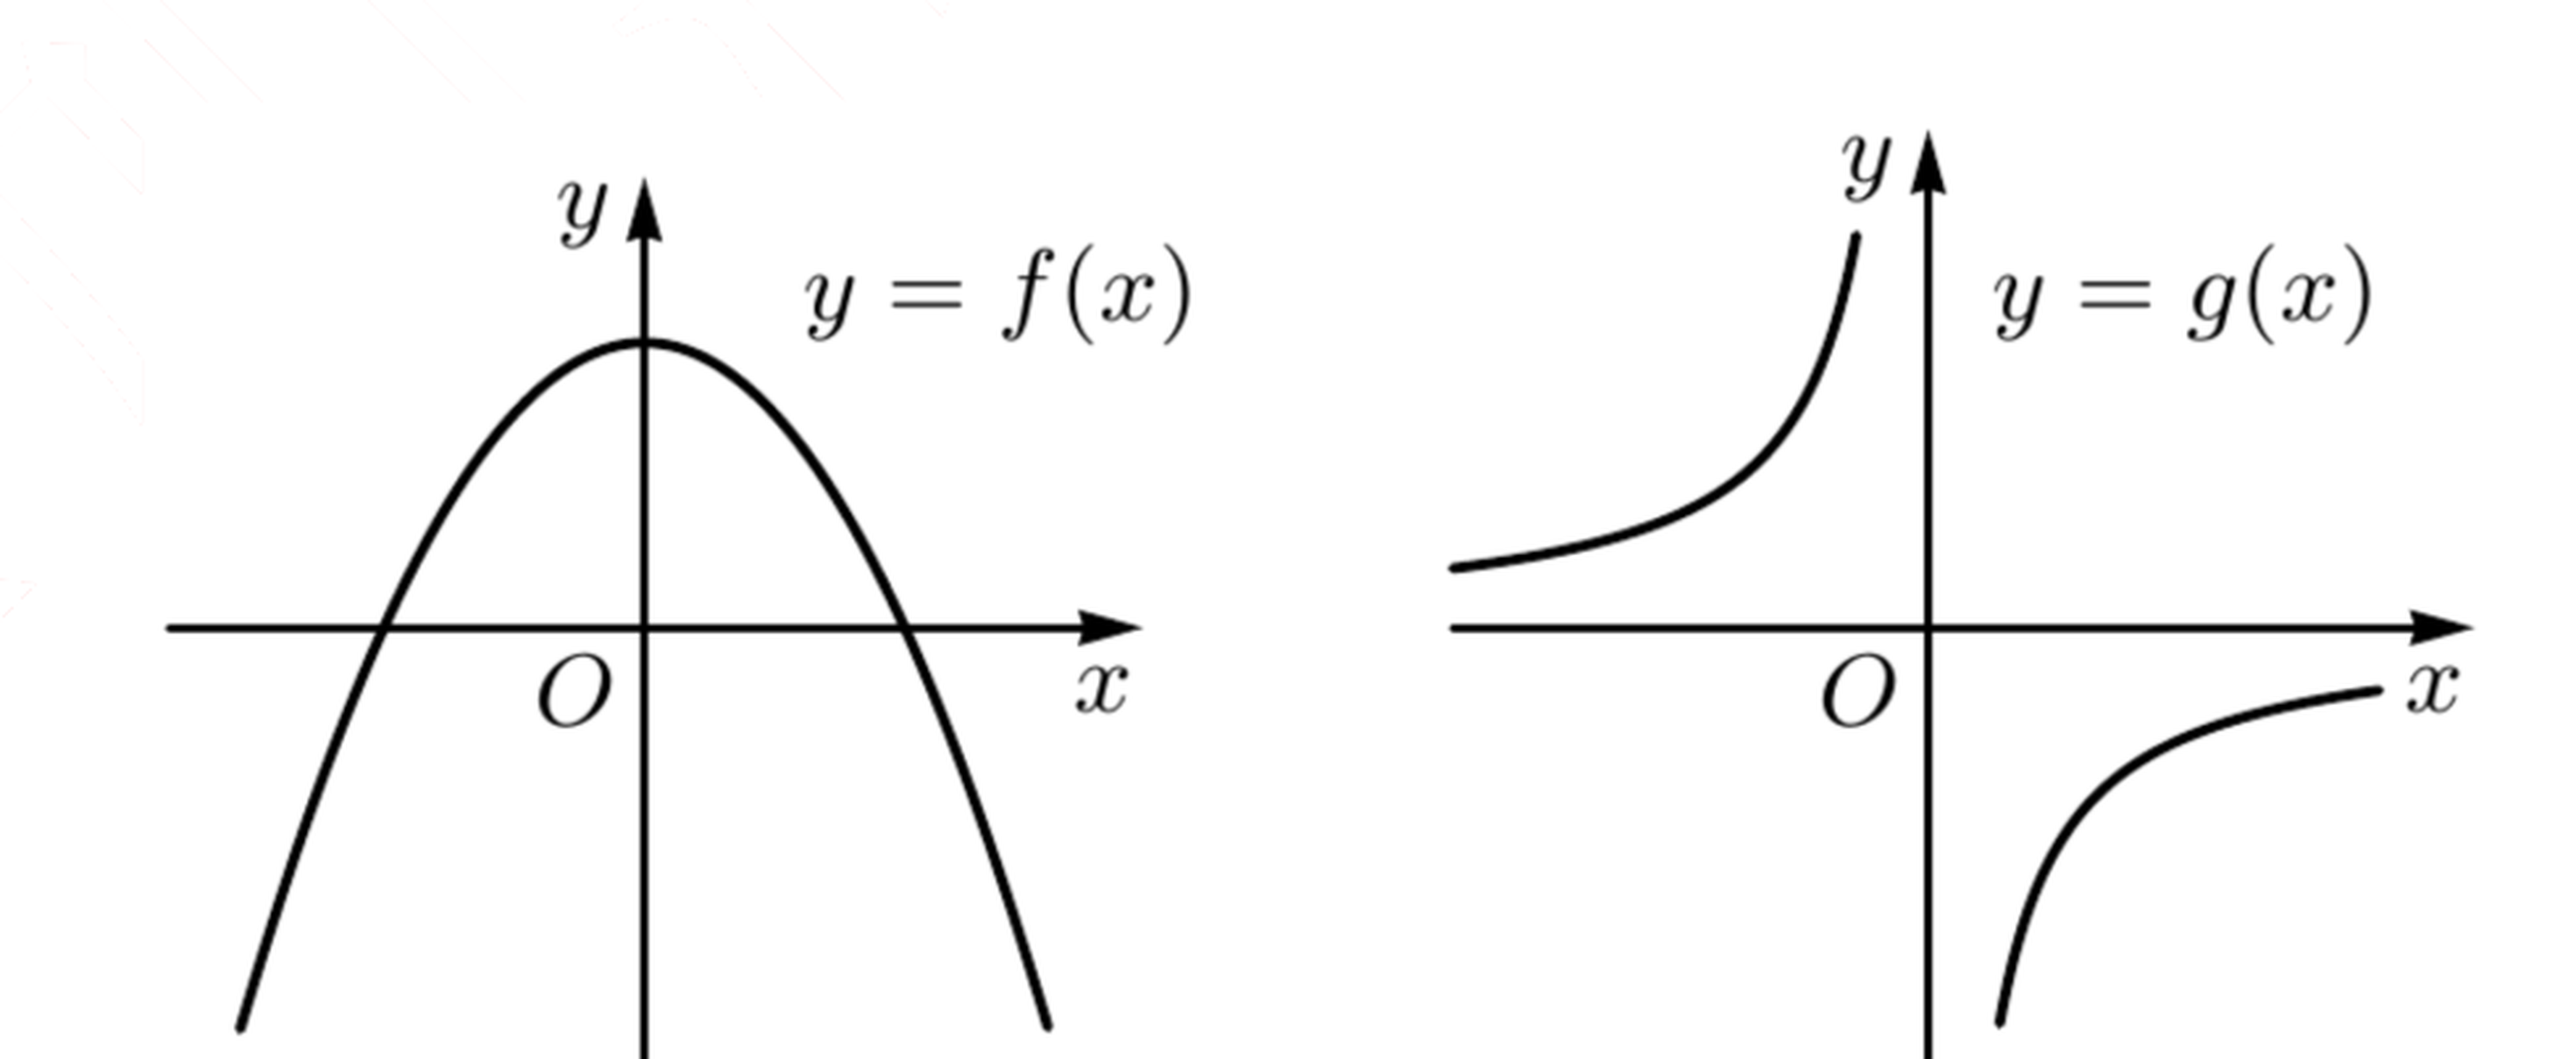
\includegraphics[width=0.72\textwidth]{figures/gao134_q13_graphs.png}\\[0.6em]
% A/B/C/D 四幅函数图象选项取原卷 04 页截图去粉色水印，按原卷一行四幅排布合并为一张
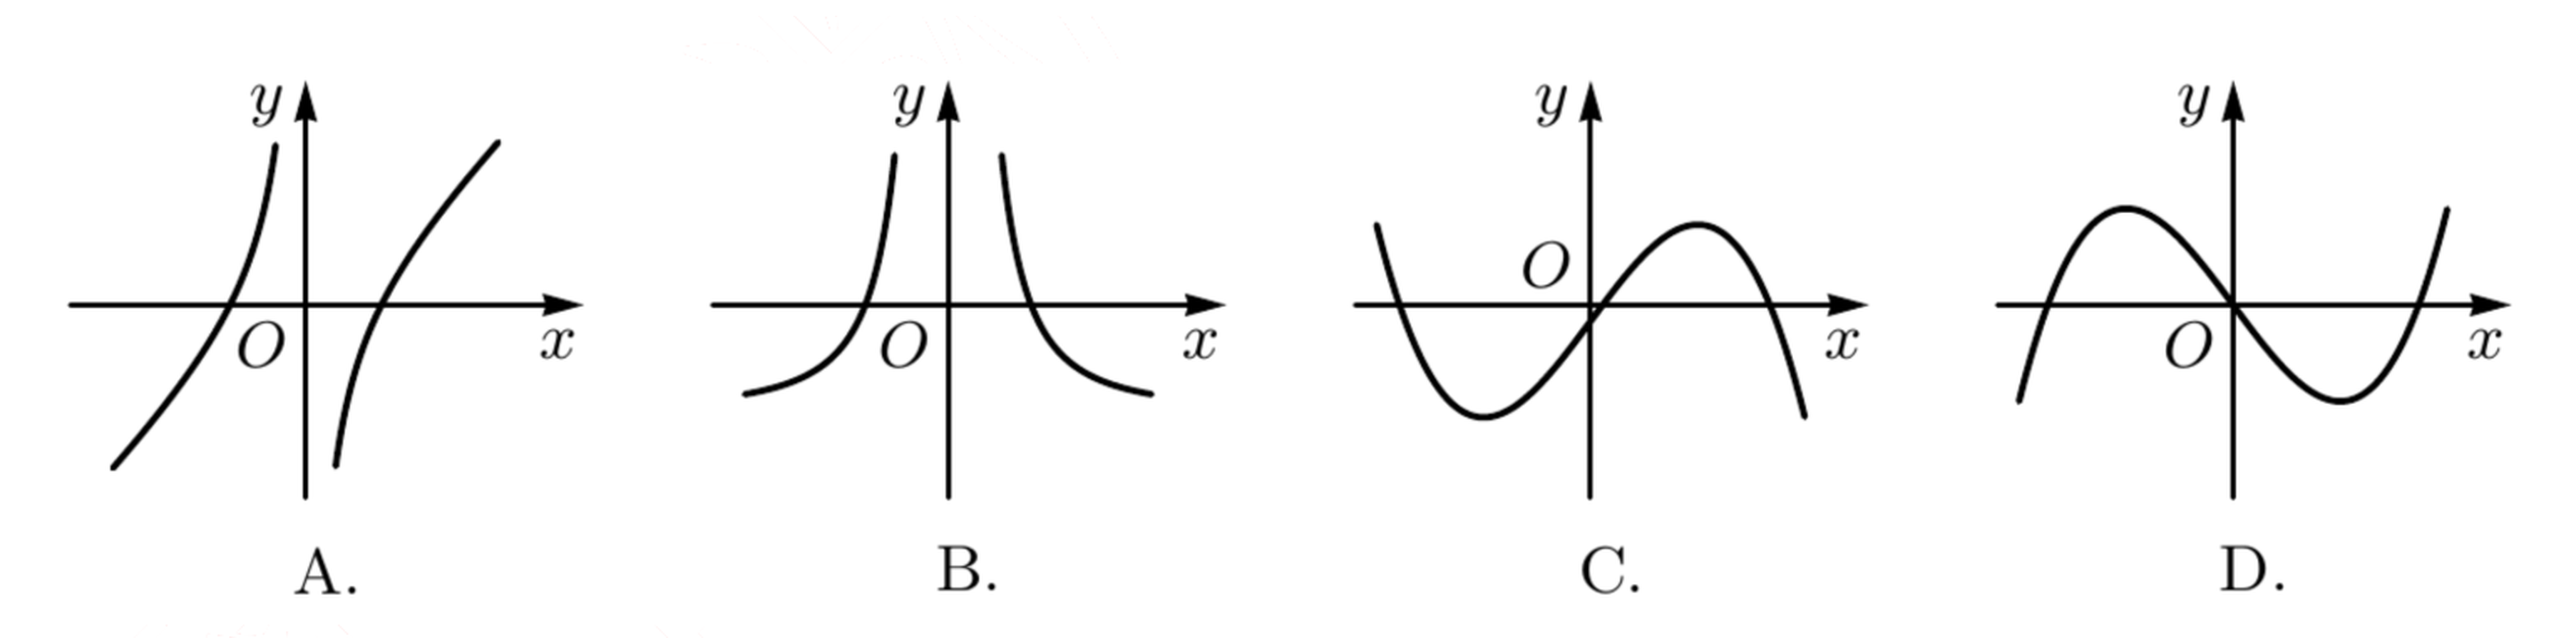
\includegraphics[width=0.90\textwidth]{figures/gao134_q13_options.png}
\end{center}

\ifanswer
\solbegin
\step{$f(x)$ 为偶函数，$g(x)$ 为奇函数，因此 $f(x)g(x)$ 为奇函数，排除 B.}
\step{又 $x=0$ 不在乘积函数的定义域内，其图象在 $y$ 轴上没有点，排除 C、D，}
\step{故选 $A$.}
\solend
\fi

\item 设全集为自然数集 $\N$，$E=\{x\mid x=2n,n\in\N\}$，$F=\{x\mid x=4n,n\in\N\}$，那么集合 $\N$ 可以表示成\mbox{（\quad）}

\keepwithprev
A. $E\cap F$\qquad\qquad B. $\overline{E}\cup F$\qquad\qquad C. $\overline{F}\cup E$\qquad\qquad D. $\overline{E}\cap\overline{F}$

\ifanswer
\solbegin
\step{$F\subseteq E$，所以 $\overline{F}\cup E=\N$，故选 $C$.}
\solend
\fi

\item 已知函数 $y=f(x)$，其中 $f(x)=x^2+bx$，则“$b<0$”是“$f(f(x))$ 的最小值与 $f(x)$ 的最小值相等”的\mbox{（\quad）}

\keepwithprev
A. 充分非必要条件\qquad\qquad B. 必要非充分条件

C. 充分必要条件\qquad\qquad D. 既非充分又非必要条件

\ifanswer
\solbegin
\step{$f(x)=\left(x+\dfrac b2\right)^2-\dfrac{b^2}4$，最小值为 $-\dfrac{b^2}4$，值域为 $\left[-\dfrac{b^2}4,+\infty\right)$.}
\step{当 $b<0$ 时，$-\dfrac b2>0\geqslant-\dfrac{b^2}4$，存在 $x$ 使 $f(x)=-\dfrac b2$，}
\step{从而 $f(f(x))$ 的最小值也为 $-\dfrac{b^2}4$，充分性成立.}
\step{当 $b=0$ 时，$f(x)=x^2$，$f(f(x))=x^4$，两者最小值均为 $0$，必要性不成立.}
\step{故选 $A$.}
\solend
\fi

\item 已知 $a,b,c\in\R$，若存在常数 $M>0$，使得 $a^2+b^2+c^2<M$，则称 $(a,b,c)$ 是有界数组. 对以下两个命题：

①若 $\lvert a^2+b+c\rvert+\lvert a^2+b-c\rvert\leqslant1$，则 $(a,b,c)$ 是有界数组；

②若 $\lvert a^2+b+c\rvert+\lvert a+b^2-c\rvert\leqslant1$，则 $(a,b,c)$ 是有界数组.% ②第二项为 \lvert a+b^2-c\rvert，与①刻意不同，照录

下列判断正确的是\mbox{（\quad）}

\keepwithprev
A. ①和②均为真命题\qquad\qquad B. ①和②均为假命题

C. ①为真命题，②为假命题\qquad D. ①为假命题，②为真命题

\ifanswer
\solbegin
\step{①取 $a=t,b=-t^2,c=0$，条件左端为 $0$，而 $a^2+b^2+c^2=t^2+t^4$ 可任意大，}
\step{故①为假命题.}
\step{②由条件，$a^2+a+b^2+b\leqslant\lvert a^2+b+c\rvert+\lvert a+b^2-c\rvert\leqslant1$.}
\step{由 $(a+1)^2+(b+1)^2\geqslant0$，得 $a^2+b^2\leqslant2(a^2+a+b^2+b)+2\leqslant4$.}
\step{又 $\lvert c\rvert\leqslant\lvert a^2+b+c\rvert+a^2+\lvert b\rvert\leqslant1+4+2=7$，故 $a^2+b^2+c^2\leqslant53<54$，}
\step{可取 $M=54$，故②为真命题.}
\step{故选 $D$.}
\solend
\fi

\end{enumerate}

\bigsec{三、解答题}

\begin{enumerate}
\setcounter{enumi}{16}

\item 已知不等式 $x^2-ax-b<0$ 的解集为 $A$，不等式 $\dfrac{3-2x}{x-1}<0$ 的解集为 $B$.

(1) 若 $a=5$，$b=-6$，求 $A\cap\overline{B}$；

(2) 若 $b=2a^2$，且 $A\cup B=B$，求实数 $a$ 的取值范围.

\ifanswer
\solbegin
\step{(1) 不等式 $\dfrac{3-2x}{x-1}<0$ 等价于 $x<1$ 或 $x>\dfrac32$，}
\step{所以 $B=(-\infty,1)\cup\left(\dfrac32,+\infty\right)$，$\overline{B}=\left[1,\dfrac32\right]$，}
\step{由 $x^2-5x+6=(x-2)(x-3)<0$，得 $A=(2,3)$，因此 $A\cap\overline{B}=\varnothing$.}
\step{(2) $A\cup B=B\Leftrightarrow A\subseteq B$，且 $x^2-ax-2a^2=(x-2a)(x+a)$，}
\step{当 $a=0$ 时，$A=\varnothing$，满足条件.}
\step{当 $a>0$ 时，$A=(-a,2a)$，$-a<0<1$，$A\subseteq B\Leftrightarrow2a\leqslant1$，得 $0<a\leqslant\dfrac12$.}
\step{当 $a<0$ 时，$A=(2a,-a)$，$2a<0<1$，$A\subseteq B\Leftrightarrow-a\leqslant1$，}
\step{得 $-1\leqslant a<0$.}
\step{因此 $a$ 的取值范围为 $\left[-1,\dfrac12\right]$.}
\solend
\fi

\item 为了在夏季降温和冬季供暖时减少能源损耗，房屋的屋顶和外墙需要建造隔热层. 某幢建筑物要建造可使用 $30$ 年的隔热层，每厘米厚的隔热层建造成本为 $9$ 万元. 该建筑物每年的能源消耗费用 $C$（万元）与隔热层厚度 $x$（cm）满足如下关系式：$C=\dfrac{k}{3x+5}$（$0\leqslant x\leqslant10$）. 若不建隔热层，每年能源消耗费用为 $8$ 万元. 设 $y$（万元）为隔热层建造费用与 $30$ 年的能源消耗费用之和.

(1) 求 $k$ 的值及 $y$ 的表达式；

(2) 隔热层修建多厚时，总费用 $y$ 最小？并求最小值.

\ifanswer
\solbegin
\step{(1) 不建隔热层时 $x=0$，$C=8$，所以 $\dfrac k5=8$，得 $k=40$.}
\step{隔热层建造费用为 $9x$ 万元，$30$ 年的能源消耗费用为 $30\times\dfrac{40}{3x+5}$ 万元.}
\step{因此 $y=9x+\dfrac{1200}{3x+5}$，$0\leqslant x\leqslant10$.}
\step{(2) 令 $t=3x+5$，则 $5\leqslant t\leqslant35$，且 $y=3t+\dfrac{1200}{t}-15$，}
\step{因为 $t>0$，由基本不等式得 $y\geqslant2\sqrt{3t\cdot\dfrac{1200}{t}}-15=105$，}
\step{当且仅当 $3t=\dfrac{1200}{t}$，即 $t=20$时取等号，此时 $x=5\in[0,10]$，}% 原卷"20"与"时"之间未留空，照录
\step{所以隔热层厚度为 $5$ cm 时，总费用最小，最小值为 $105$ 万元.}
\solend
\fi

\item 已知 $f(x)=ax^2+\dfrac1x$，其中 $a$ 为常数.

(1) 若 $a\in(1,3)$，判断函数 $y=f(x)$ 在 $[1,2]$ 上的单调性，并用定义证明；

(2) 求函数 $y=f(x)-x-\dfrac1x$ 在 $[1,2]$ 上的最大值 $g(a)$.

\ifanswer
\solbegin
\step{(1) 任取 $x_1,x_2\in[1,2]$，且 $x_1<x_2$，}
\step{则 $f(x_2)-f(x_1)=(x_2-x_1)\left[a(x_1+x_2)-\dfrac1{x_1x_2}\right]$，}
\step{由 $a>1$，$x_1+x_2\geqslant2$，$x_1x_2\geqslant1$，得 $a(x_1+x_2)-\dfrac1{x_1x_2}>2-1>0$，}
\step{因此 $f(x_2)>f(x_1)$，$f(x)$ 在 $[1,2]$ 上为严格增函数.}
\step{(2) 令 $h(x)=f(x)-x-\dfrac1x=ax^2-x$，其中 $x\in[1,2]$.}
\step{若 $a=0$，则 $h(x)=-x$，所以 $h(x)_{max}=h(1)=-1$；}
\step{若 $a<0$，二次函数的图象的对称轴为 $x=\dfrac1{2a}<0$，}
\step{所以 $y=h(x)$ 在 $[1,2]$ 上是严格减函数，所以 $h(x)_{max}=h(1)=a-1$；}
\step{若 $a>0$ 且 $\dfrac1{2a}>\dfrac32$，即 $0<a<\dfrac13$ 时，$h(x)_{max}=h(1)=a-1$.}
\step{若 $a>0$ 且 $\dfrac1{2a}\leqslant\dfrac32$，即 $a\geqslant\dfrac13$ 时，$h(x)_{max}=h(2)=4a-2$.}
\step{综上所述，$g(a)=\begin{cases}a-1,a<\dfrac13\\4a-2,a\geqslant\dfrac13\end{cases}$.}
\solend
\fi

\item 已知 $f(x)=\dfrac{ax^2+1}{bx+c}$（$a,b,c\in\Z$）.

(1) 若函数 $y=f(x)$ 是奇函数，且 $f(1)=2$，$f(2)<3$，求 $a,b,c$ 的值；

(2) 若函数 $y=f(x)$ 是偶函数，且 $ac<0$，$f(2a^2+a+1)<f(-3a^2+2a-1)$，求 $a$ 的值；

(3) 若 $b=a+c^2$，且满足不等式 $\lvert f(x)\rvert\geqslant1$ 的 $x$ 的最大值为 $0$，求 $c$ 的值.

\ifanswer
\solbegin
\step{(1) 由 $f(-x)=-f(x)$，交叉相乘得 $2c(ax^2+1)=0$ 恒成立，}
\step{因此 $c=0$，$b\neq0$.}
\step{由 $f(1)=2$，得 $a+1=2b$，}
\step{于是 $f(2)=\dfrac{4a+1}{2b}=4-\dfrac3{2b}<3\Leftrightarrow0<b<\dfrac32$，}
\step{因为 $b\in\Z$，所以 $b=1$，进而 $a=1$，$c=0$.}
\step{(2) 由 $f(-x)=f(x)$，交叉相乘得 $2bx(ax^2+1)=0$ 恒成立，因此 $b=0$.}
\step{此时 $f(x)=\dfrac ac x^2+\dfrac1c$，且 $\dfrac ac<0$.}
\step{设 $u=2a^2+a+1$，$v=-3a^2+2a-1$.}
\step{方程 $2a^2+a+1=0$ 与 $3a^2-2a+1=0$ 的判别式分别为 $-7$ 与 $-8$，}
\step{都小于 $0$，所以 $u>0$，$v<0$.}
\step{于是 $f(u)<f(v)\Leftrightarrow u^2>v^2\Leftrightarrow u>-v\Leftrightarrow-a^2+3a>0\Leftrightarrow0<a<3$，}
\step{因为 $a\in\Z$，所以 $a=1$ 或 $a=2$.}
\step{(3) 因为解集的最大值为 $0$，所以 $f(0)$ 有定义且 $\lvert f(0)\rvert\geqslant1$，}
\step{即 $c\neq0$，$\left\lvert\dfrac1c\right\rvert\geqslant1$，结合 $c\in\Z$，得 $c=\pm1$，从而 $b=a+1$.}
\step{当 $x=2$ 时，分母 $2a+2+c$ 为奇数，必不为 $0$；}
\step{又因为 $2>0$，必须有 $\lvert f(2)\rvert<1\Leftrightarrow\lvert4a+1\rvert<\lvert2a+2+c\rvert$，}
\step{若 $c=-1$，则 $(4a+1)^2<(2a+1)^2\Leftrightarrow4a(3a+1)<0\Leftrightarrow-\dfrac13<a<0$，}
\step{不存在满足条件的整数 $a$.}
\step{若 $c=1$，则 $(4a+1)^2<(2a+3)^2\Leftrightarrow4(3a+2)(a-1)<0\Leftrightarrow-\dfrac23<a<1$，}
\step{所以 $a=0$，$b=1$，此时 $f(x)=\dfrac1{x+1}$，}
\step{且 $\lvert f(x)\rvert\geqslant1\Leftrightarrow0<\lvert x+1\rvert\leqslant1\Leftrightarrow x\in[-2,-1)\cup(-1,0]$，}
\step{解集的最大值确为 $0$，因此 $c=1$.}
\solend
\fi

\item 已知函数 $y=f(x)$ 的定义域为 $\R$，且当 $x>0$ 时，$f(x)=\dfrac1{x+1}$. 对任意 $x_0\in\R$，定义集合 $D(x_0)=\{d\mid f(x_0+d)>f(x_0)\}$.

(1) 若当 $x\leqslant0$ 时，$f(x)=-2x+1$，求函数 $y=f(x)$ 的值域；

(2) 若 $y=f(x)$ 是偶函数，且 $f(0)=1$，求证：$D(-2)=\{-d\mid d\in D(2)\}$；

(3) 若 $y=f(x)$ 是奇函数，且 $x_1x_2\neq0$，求证：“$f(x_1)\leqslant f(x_2)$”的充要条件是\!\mbox{“$D(x_2)\subseteq D(x_1)$”}.

\ifanswer
\solbegin
\step{(1) 当 $x>0$ 时，$0<f(x)<1$；当 $x\leqslant0$ 时，$f(x)=-2x+1\geqslant1$.}
\step{函数的值域为 $(0,1)\cup[1,+\infty)=(0,+\infty)$.}
\step{(2) 由 $f(x)$ 是偶函数及 $f(0)=1$，得 $f(x)=\dfrac1{1+\lvert x\rvert}$，且 $f(2)=f(-2)=\dfrac13$.}
\stepm{法一：}{$D(2)=\left\{d\mid\dfrac1{1+\lvert2+d\rvert}>\dfrac13\right\}=\{d\mid\lvert2+d\rvert<2\}=(-4,0)$，}
\step{$D(-2)=\left\{d\mid\dfrac1{1+\lvert-2+d\rvert}>\dfrac13\right\}=\{d\mid\lvert-2+d\rvert<2\}=(0,4)$，}
\step{因此 $\{-d\mid d\in D(2)\}=(0,4)=D(-2)$.}
\stepm{法二：}{任取 $d\in D(-2)$，由定义得 $f(-2+d)>f(-2)$.}
\step{因为 $y=f(x)$ 是偶函数，所以对任意的实数 $x$，有 $f(-x)=f(x)$，}
\step{因此 $f(-2+d)=f(-(-2+d))=f(2-d)$，且 $f(-2)=f(2)$.}
\step{所以不等式 $f(-2+d)>f(-2)$ 等价于 $f(2-d)>f(2)$，}
\step{这恰好是 $-d\in D(2)$ 的定义，}
\step{所以 $d\in D(-2)\Leftrightarrow-d\in D(2)$，故 $D(-2)=\{-d\mid d\in D(2)\}$.}
\step{(3) 由 $f(x)$ 是奇函数，得 $f(0)=0$；}
\step{当 $x<0$ 时，$f(x)=-f(-x)=-\dfrac1{1-x}=\dfrac1{x-1}$；}
\step{所以 $f(x)=\begin{cases}\dfrac1{x-1},&x<0\\0,&x=0;\\\dfrac1{x+1},&x>0\end{cases}$}
% 2026-11-15 回原图订正：原卷 11 页此 cases 块末无句点，本稿初转顺手补了西文句点，今删去（Q19 08 页同类块末有句点，照录保留）。
\step{当 $x_0<0$ 时，$D(x_0)=\{d\mid f(x_0+d)>f(x_0)\}=(-\infty,0)\cup[-x_0,+\infty)$，}
\step{当 $x_0=0$ 时，$D(0)=\{d\mid f(0+d)>f(0)\}=(0,+\infty)$，}
\step{当 $x_0>0$ 时，$D(x_0)=\{d\mid f(x_0+d)>f(x_0)\}=(-x_0,0)$.}
\stepm{先证明必要性.}{若 $f(x_1)\leqslant f(x_2)$，仅需讨论三类情形：}
\step{若 $x_2\leqslant x_1<0$，}
\step{则 $D(x_1)=(-\infty,0)\cup[-x_1,+\infty),D(x_2)=(-\infty,0)\cup[-x_2,+\infty)$，}
\step{故 $D(x_2)\subseteq D(x_1)$；}
\step{若 $0<x_2\leqslant x_1$，则 $D(x_1)=(-x_1,0),D(x_2)=(-x_2,0)$，}
\step{故 $D(x_2)\subseteq D(x_1)$；}
\step{若 $x_1<0<x_2$，则 $D(x_1)=(-\infty,0)\cup[-x_1,+\infty),D(x_2)=(-x_2,0)$，}
\step{故 $D(x_2)\subseteq D(x_1)$.}
\stepm{再证明充分性.}{若 $D(x_2)\subseteq D(x_1)$，}
\step{若 $x_1<0,x_2<0$，}
\step{则 $D(x_1)=(-\infty,0)\cup[-x_1,+\infty),D(x_2)=(-\infty,0)\cup[-x_2,+\infty)$，}
\step{由 $D(x_2)\subseteq D(x_1)$ 得 $x_2\leqslant x_1$，}
\step{又 $y=f(x)$ 在 $(-\infty,0)$ 上是严格减函数，所以 $f(x_1)\leqslant f(x_2)$；}
\step{若 $x_1>0,x_2>0$，则 $D(x_1)=(-x_1,0),D(x_2)=(-x_2,0)$，}
\step{由 $D(x_2)\subseteq D(x_1)$ 得 $x_2\leqslant x_1$，}
\step{又 $y=f(x)$ 在 $(0,+\infty)$ 上是严格减函数，所以 $f(x_1)\leqslant f(x_2)$；}
\step{若 $x_1<0,x_2>0$，则 $f(x_1)<0<f(x_2)$，结论成立；}
\step{若 $x_1>0,x_2<0$，此时 $D(x_1)=(-x_1,0)$ 中只有负数，}
\step{而 $D(x_2)=(-\infty,0)\cup[-x_2,+\infty)$ 中有正数，$D(x_2)\subseteq D(x_1)$ 不成立.}
\step{综上，“$f(x_1)\leqslant f(x_2)$”的充要条件是“$D(x_2)\subseteq D(x_1)$”.}
\solend
\fi

\end{enumerate}

\end{document}
"
% 紧凑版：xelatex "\def\iscompact{1}% 高一134_华师大二附中_期中.tex
%   —— 高一上数学"2026-2027 年华师大二附中高一上期中"（试卷版/答案版）
% 试卷版：xelatex 高一134_华师大二附中_期中.tex
% 答案版：xelatex "\def\isanswer{1}\input{高一134_华师大二附中_期中.tex}"
% 紧凑版：xelatex "\def\iscompact{1}\input{高一134_华师大二附中_期中.tex}"
%
% ① 原始材料：微信公众号"魔都数学加油站"文章，作者破晓，2026-11-15 18:04 发布；
% 连载"27学年高一134"，原文标题"27学年高一134——2026-2027年上海市华师大二附中高一上期中"；
% 原文链接：https://mp.weixin.qq.com/s/bQlkmlGdCtAlytY331vf3g。
% 正文为 13 张 PNG 页（01、04、06、08、09、10、11、12、13 为 2560x3620；
% 02、03、05、07 为 4762x6735，同一篇各页分辨率不同，逐页按各自分辨率裁图核对），
% 题目下印有【解析】，为讲评版。题目、解析均据原图转录；卷面粉红色水印
% "魔都数学加油站"及公众号页脚未录入。
% 全卷 2 幅插图，均在第 04 页：第 13 题题干 y=f(x)、y=g(x) 两幅函数图象合并裁为
% figures/gao134_q13_graphs.png，第 13 题 A/B/C/D 四幅函数图象选项合并裁为
% figures/gao134_q13_options.png；两图均取原卷 04 页截图 3× LANCZOS 放大、
% 白化粉色水印（只白化浅粉色 R>175 且 G>140 且 B>140 的像素，保留红色标签）。
% 注意：本卷 Q13 四幅选项在原卷排为"一行四幅"（1×4），并非 高一132 第 14 题
% 的 2×2 排布，本稿按原卷 1×4 合并裁为一张，不重排、不用 TikZ 重绘。
%
% 卷首标题：原卷印作"2026-2027 年华师大二附中高一上期中"（公众号标题中的"上海市"
% 卷面标题行没有，本稿照卷面），年份区间按全稿惯例排 en dash；原卷未印副标题，
% 本卷为期中卷、跨集合与常用逻辑用语／不等式／函数三章，按题目内容标为
% "集合与常用逻辑用语、不等式、函数"（与 125／126／128／129／131／132／133 同期中卷口径相同）：
% 集合与逻辑见 Q6、Q10、Q14、Q16、Q17、Q21，不等式见 Q3、Q7、Q9、Q11、Q15、Q18、Q19，
% 函数（函数性质、二分法、奇偶性、基本不等式应用）见 Q4、Q5、Q8、Q12、Q13、Q20。
%
% 题号体例：本卷共 19 题——一、填空题 3—12（10 题）、二、选择题 13—16（4 题）、
% 三、解答题 17—21（5 题）。三节分别 \setcounter{enumi}{2}／{12}／{16}。
% 第 13 页仅为 Q21 (3) 解析续尾，全卷无「四、附加题」。
%
% ② 与原卷的排版差异：
%   ① 原文从第 3 题起，本稿保留原题号（见上"题号体例"）；
%   ② 原卷每题下直接印【解析】，本稿按全稿惯例置于答案版；第 13—16 题答案均在
%      解析末句"故选 …"，题干括号内留空、不另提 \ans{}（四题均无独立答案段）；
%      全卷无只印括号内答案、无解析的选择题；
%   ③ 原卷未印副标题，本稿按"知识模块"口径补出；
%   ④ 原卷填空横线按全稿惯例排为 \blankline[4.4em]；选择题括号排 \mbox{（\quad）}、
%      每个选项段前按惯例加 \keepwithprev（Q13 四选项为图，守卫前行为 \begin{center}；
%      Q15、Q16 四选项分两行排，\keepwithprev 只加在 A. 行前）；解答题不留作答区、
%      不加 \anspace（原卷为讲评版，与 129／131／132／133 同）；
%   ⑤ 原卷数集印黑板粗体（Q7／Q11／Q12／Q16／Q21 的 R、Q14／Q20 的 N、Q20 的 Z），
%      按全稿惯例统一排 \R／\N／\Z；绝对值排 \lvert…\rvert，集合描述竖线排 \mid；不等号按全稿惯例排
%      \leqslant／\geqslant；补集照原卷上划线排 \overline{B}、\overline{E}、\overline{F}；
%   ⑥ 子题标号 (1)(2)(3) 与括注原卷均用半角括号，照录（与 131／132／133 同）；
%      圈数字 ①② 照录；原卷 Q21 (2) 解析"法一：""法二："与 Q21 (3) 解析
%      "先证明必要性.""再证明充分性."四处标签印红色加粗，按 高一53／108／133 成例排
%      \stepm{法一：}／\stepm{法二：}／\stepm{先证明必要性.}／\stepm{再证明充分性.}
%      （加粗着色、不引入红色，不动 common.sty）；Q8 解析"第 1 步：""第 2 步：""
%      "第 3 步："原卷印黑色常规宋体（非红非粗），照录为普通 \step 行内文字；
%   ⑦ 数学式内半角逗号照录（如 Q6 $A=\{0,1,2,3\}$、Q14 $x=2n,n\in\N$、
%      Q16 $a,b,c\in\R$ 与 $a=t,b=-t^2,c=0$、Q19 $x_1,x_2\in[1,2]$、
%      Q20 $a,b,c\in\Z$、Q21 $x_1<0,x_2<0$ 与 $D(x_1)=(-x_1,0),D(x_2)=(-x_2,0)$）；
%      原卷行末全角句点按全稿惯例从宽排西文句点；cases 块末的句点逐处照录：
%      Q19 解析（08 页）块末原卷有句点照录、Q21 (3) 解析（11 页）块末原卷无句点不补，
%      两处原卷自身不统一（2026-11-15 回原图核对，本稿初转曾顺手补句点，已删去）；
%   ⑧ 原卷 Q8 解析跨 01—02 页、Q10 解析跨 02—03 页、Q12 解析跨 03—04 页、
%      Q16 解析跨 05—06 页、Q17 解析跨 06—07 页、Q20 解析跨 08—10 页、
%      Q21 解析跨 10—13 页，本稿按题合并连续排版；末页第 13 页为
%      Q21 (3) 解析续尾与"综上"一句，按实际印刷行单列；
%   ⑨ 题干中的中文弯引号按原卷照录（Q10 研究问题、Q15 条件、Q21 (3) 充要条件），
%      注释内一律 ASCII 引号。
%
% 判别式字形：全卷仅 Q9 解析末行出现一处判别式记号
%   "两值均满足 $\Delta=p^2-4p=18\mp12\sqrt2>0$"，逐处放大核对，原卷印高三角
%   $\Delta$（等腰、高，实测高宽比约 1.14），照录 \Delta；卷内无扁三角 \triangle，
%   与 高一132 同题排 $\triangle$、高一133 部分判别式排 $\triangle$ 均不同。
%
% 子集符号：Q6 题干 $C\subseteq A$、$C\subseteq B$ 与解析 $C\subseteq A\cap B$、
%   Q14 解析 $F\subseteq E$、Q17 解析 $A\subseteq B$、Q21 题干与解析各处的
%   $D(x_2)\subseteq D(x_1)$，全部印带下划线的 $\subseteq$，逐处放大核对，
%   照录 \subseteq；全卷未出现单线 \subset。
%
% 原卷存疑照录（均照录未改，正文对应处另有 % 注）：
%   第 6 题题干集合 $A=\{0,1,2,3\}$ 三个逗号后不留空，紧邻的 $B=\{0,2,4,5\}$
%      三个逗号后却留空，同卷同一行两集合排字不一，照录其逗号均为半角；
%   第 16 题命题②作 $\lvert a^2+b+c\rvert+\lvert a+b^2-c\rvert\leqslant1$，
%      与命题①第二项 $\lvert a^2+b-c\rvert$ 不同（①无 $b$ 的平方、②有），
%      两命题刻意不同，照录；解析"②由条件，$a^2+a+b^2+b\leqslant\cdots$"
%      由两项相加直接得到，照录；
%   第 18 题 (2) 解析"即 $t=20$时取等号"中"20"与"时"之间原卷未留空，照录；
%   第 19 题解析 $h(x)_{max}$ 的"max"下标三处字形不一（斜体／正体混排），照录；
%   第 20 题 (1)(2) 解析"由 $f(-x)=-f(x)$，交叉相乘得……"与"由 $f(-x)=f(x)$，
%      交叉相乘得……"两处措辞照录；
%   第 21 题 (2) 原卷并存"法一"（集合计算）与"法二"（定义推证）两套证明，照录不删。
%
% 行数复核：逐题数 \step/\stepm 条数，合计 134 条（Q3：2；Q4：1；Q5：1；Q6：1；
% Q7：2；Q8：4；Q9：3；Q10：4；Q11：5；Q12：8；Q13：3；Q14：1；Q15：5；
% Q16：7；Q17：9；Q18：7；Q19：11；Q20：22；Q21：38），与原卷印刷行逐题相等
% （cases 块作一个印刷行计）。第 13—16 题答案在解析末句，括号内留空、不另提 \ans{}；
% 第 21 题四条 \stepm 计入 38 条内。
%
\documentclass[a4paper,11pt]{article}
\usepackage{common}

\begin{document}

\examtitlest[3]{2026--2027 年华师大二附中高一上期中}{集合与常用逻辑用语、不等式、函数}

\bigsec{一、填空题}

\begin{enumerate}
\setcounter{enumi}{2}

\item 不等式 $\lvert 2x+1\rvert\geqslant3$ 的解集为\blankline[4.4em].

\ifanswer
\solbegin
\step{$\lvert 2x+1\rvert\geqslant3\Leftrightarrow 2x+1\leqslant-3$ 或 $2x+1\geqslant3\Leftrightarrow x\leqslant-2$ 或 $x\geqslant1$，}
\step{故解集为 $(-\infty,-2]\cup[1,+\infty)$.}
\solend
\fi

\item 函数 $y=\sqrt{x+1}+\dfrac1x$ 的定义域为\blankline[4.4em].

\ifanswer
\solbegin
\step{$x+1\geqslant0$ 且 $x\neq0$，得定义域为 $[-1,0)\cup(0,+\infty)$.}
\solend
\fi

\item 已知等式 $3x^2-4x-2=a(x-1)^2+b(x-1)+c$ 恒成立，其中 $a$、$b$、$c$ 为常数，则 $a-b+c=$\blankline[4.4em].

\ifanswer
\solbegin
\step{令 $x=0$，得 $a-b+c=-2$.}
\solend
\fi

\item 已知集合 $A=\{0,1,2,3\}$，$B=\{0,2,4,5\}$，$C\subseteq A$，$C\subseteq B$，符合条件的集合 $C$ 有\blankline[4.4em]个.% 原卷 A 的逗号后不留空、B 的逗号后留空，排字不一，照录

\ifanswer
\solbegin
\step{$C\subseteq A\cap B=\{0,2\}$，所以符合条件的集合 $C$ 有 $2^2=4$ 个.}
\solend
\fi

\item 设 $a$、$b\in\R$，且 $a^2+4b^2=2$，则 $ab$ 的最大值为\blankline[4.4em].

\ifanswer
\solbegin
\step{$(a-2b)^2=a^2+4b^2-4ab=2-4ab\geqslant0$，得 $ab\leqslant\dfrac12$，}
\step{当且仅当 $a=2b=\pm1$ 时取等号，故 $ab$ 的最大值为 $\dfrac12$.}
\solend
\fi

\item 已知函数 $y=x(13-2x)^2-140$，用二分法求函数在区间 $(3,4)$ 上的零点时，第 3 步应计算 $x=$\blankline[4.4em]的函数值.

\ifanswer
\solbegin
\step{记 $f(x)=x(13-2x)^2-140$，则 $f(3)=7>0$，$f(4)=-40<0$.}
\step{第 1 步：$f\left(\dfrac72\right)=-14<0$，区间缩小为 $\left(3,\dfrac72\right)$.}
\step{第 2 步：$f\left(\dfrac{13}4\right)=-\dfrac{43}{16}<0$，区间缩小为 $\left(3,\dfrac{13}4\right)$.}
\step{第 3 步：应计算 $x=\dfrac{3+\frac{13}4}2=\dfrac{25}8$ 的函数值.}
\solend
\fi

\item 已知一元二次方程 $x^2+px+p=0$ 的两个实根分别为 $x_1$、$x_2$，且 $x_1^2x_2+x_2^2x_1=-18$，则 $p=$\blankline[4.4em].% 判别式 \Delta 高三角，逐处放大核对

\ifanswer
\solbegin
\step{由韦达定理，$x_1+x_2=-p$，$x_1x_2=p$，}
\step{则 $x_1^2x_2+x_2^2x_1=x_1x_2(x_1+x_2)=-p^2=-18\Rightarrow p=\pm3\sqrt2$，}
\step{两值均满足 $\Delta=p^2-4p=18\mp12\sqrt2>0$，故 $p=\pm3\sqrt2$.}
\solend
\fi

\item 研究问题：“已知关于 $x$ 的不等式 $ax^2-bx+c>0$ 的解集为 $(1,2)$，解关于 $x$ 的不等式 $cx^2-bx+a>0$”，有如下解法：

解：由 $ax^2-bx+c>0\Rightarrow a-b\left(\dfrac1x\right)+c\left(\dfrac1x\right)^2>0$，令 $y=\dfrac1x$，则 $y\in\left(\dfrac12,1\right)$，

所以不等式 $cx^2-bx+a>0$ 的解集为 $\left(\dfrac12,1\right)$.

参考上述解法，已知关于 $x$ 的不等式 $\dfrac{k}{x+a}+\dfrac{x+b}{x+c}<0$ 的解集为 $(-3,-1)\cup(2,4)$，则关于 $x$ 的不等式 $\dfrac{kx}{ax-1}+\dfrac{bx-1}{cx-1}<0$ 的解集为\blankline[4.4em].

\ifanswer
\solbegin
\step{当 $x=0$ 时，所求不等式左端为 $1$，不满足不等式.}
\step{当 $x\neq0$ 时，两个分式的分子、分母同除以 $x$，得 $\dfrac{k}{a-\frac1x}+\dfrac{b-\frac1x}{c-\frac1x}<0$.}
\step{令 $t=-\dfrac1x$，则所求不等式化为 $\dfrac{k}{t+a}+\dfrac{t+b}{t+c}<0$，即 $-\dfrac1x\in(-3,-1)\cup(2,4)$，}
\step{解得 $x\in\left(-\dfrac12,-\dfrac14\right)\cup\left(\dfrac13,1\right)$.}
\solend
\fi

\item 已知 $a\in(0,+\infty)$，若对任意的 $x\in(0,+\infty)$，均有 $\lvert x^2-a\rvert+\lvert x+b\rvert=\lvert x^2+x-a+b\rvert$，则 $a^2-b^2$ 的最小值为\blankline[4.4em].

\ifanswer
\solbegin
\step{原等式成立的充要条件是 $(x^2-a)(x+b)\geqslant0$.}
\step{当 $0<x<\sqrt a$ 时须有 $x+b\leqslant0$；当 $x>\sqrt a$ 时须有 $x+b\geqslant0$，因此 $b=-\sqrt a$.}
\step{此时 $(x^2-a)(x+b)=(x+\sqrt a)(x-\sqrt a)^2\geqslant0$，满足题意.}
\step{$a^2-b^2=a^2-a=\left(a-\dfrac12\right)^2-\dfrac14\geqslant-\dfrac14$，}
\step{当 $a=\dfrac12$，$b=-\dfrac{\sqrt2}2$ 时取等号，最小值为 $-\dfrac14$.}
\solend
\fi

\item 已知函数 $y=f(x)$ 在 $\R$ 上是严格增函数，当 $x\neq0$ 且 $f(x)\neq0$ 时，满足 $f(x)\cdot f\left[\dfrac1{f(x)}+\dfrac1x\right]=1$，则 $f(1)=$\blankline[4.4em].

\ifanswer
\solbegin
\step{当 $xf(x)>0$ 时，记 $t=\dfrac1{f(x)}+\dfrac1x\neq0$，则 $f(t)=\dfrac1{f(x)}\neq0$.}
\step{将 $t$ 代入题设，得 $f\left(f(x)+\dfrac1t\right)=f(x)$，严格增性给出 $f(x)+\dfrac1t=x$，}
\step{化简得 $f(x)^2+xf(x)-x^2=0$，由 $\dfrac{f(x)}x>0$ 得 $f(x)=\dfrac{\sqrt5-1}2x$.}
\step{设 $a=f(0)$，若 $a>0$，则 $f(a)>f(0)=a>0$；}
\step{若 $a<0$，则 $f(a)<f(0)=a<0$.}
\step{两种情形都有 $af(a)>0$ 且 $\dfrac{f(a)}a>1$，与上式 $\dfrac{f(a)}a=\dfrac{\sqrt5-1}2<1$ 矛盾，}
\step{因此 $f(0)=0$.}
\step{于是 $f(1)>0$，代入上式得 $f(1)=\dfrac{\sqrt5-1}2$.}
\solend
\fi

\end{enumerate}

% 第 13 题是"节标题 + 题干 + 两幅图 + 四幅选项图"约 15cm 的整块，
% 守卫只放在 \bigsec 之前；若再在 \item 之前放第二枚，会在标题已印出后才触发换页，
% 把题目推走、留下孤立节标题（切页审计 B 类）。高度须覆盖整块。
\needvspace{16cm}
\bigsec{二、选择题}

\begin{enumerate}
\setcounter{enumi}{12}

\item 已知函数 $y=f(x)$ 与 $y=g(x)$ 的图象如图所示，则函数 $y=f(x)\cdot g(x)$ 的图象可能是\mbox{（\quad）}

\keepwithprev
\begin{center}
% 题干 y=f(x)、y=g(x) 两幅函数图象取原卷 04 页截图去粉色水印，按原卷左右排布合并为一张
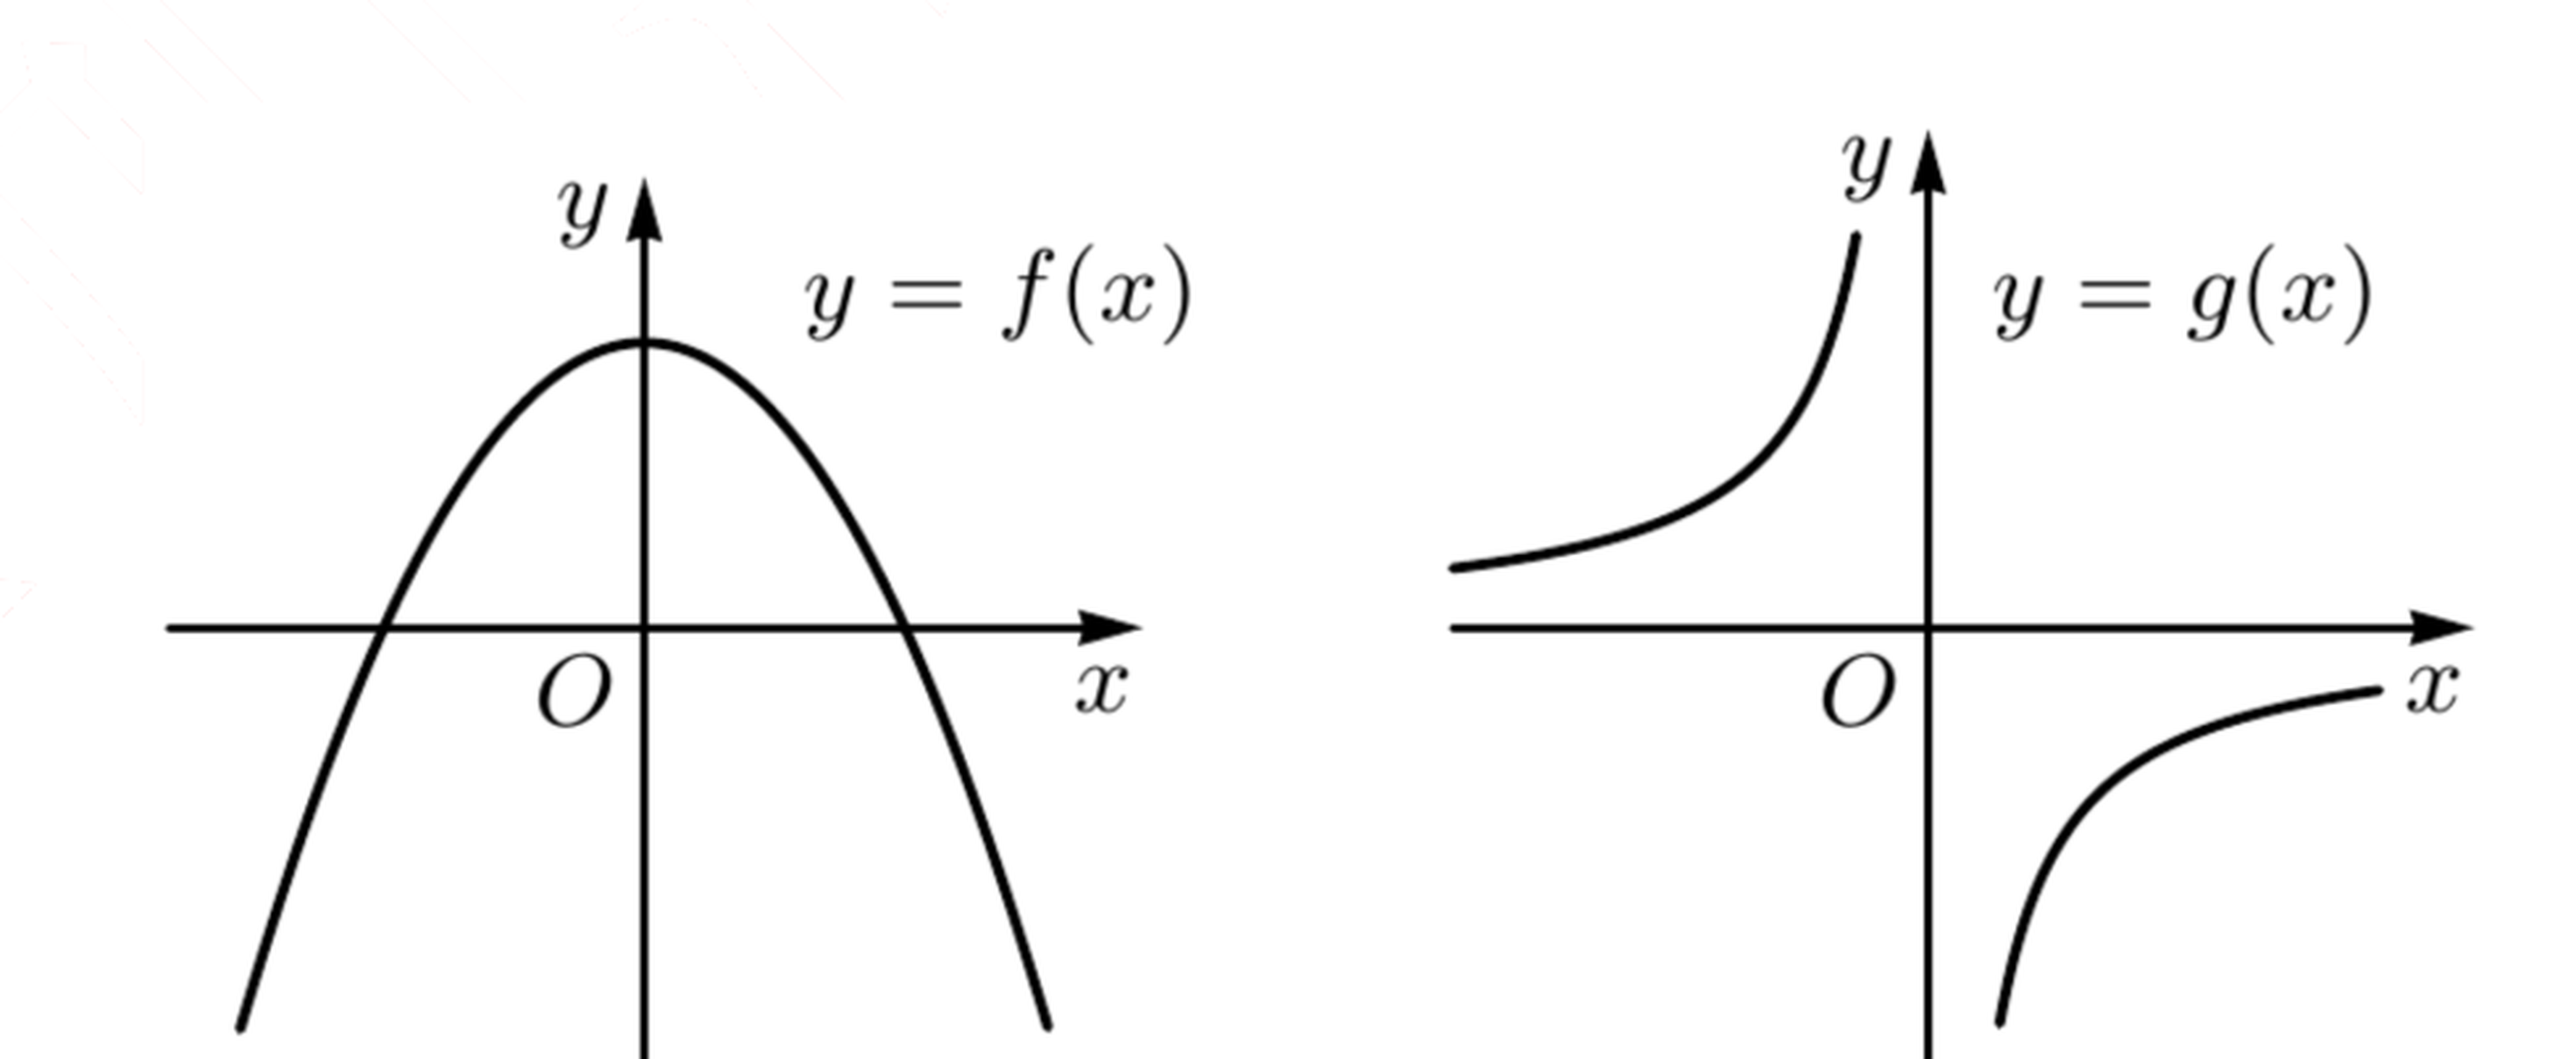
\includegraphics[width=0.72\textwidth]{figures/gao134_q13_graphs.png}\\[0.6em]
% A/B/C/D 四幅函数图象选项取原卷 04 页截图去粉色水印，按原卷一行四幅排布合并为一张
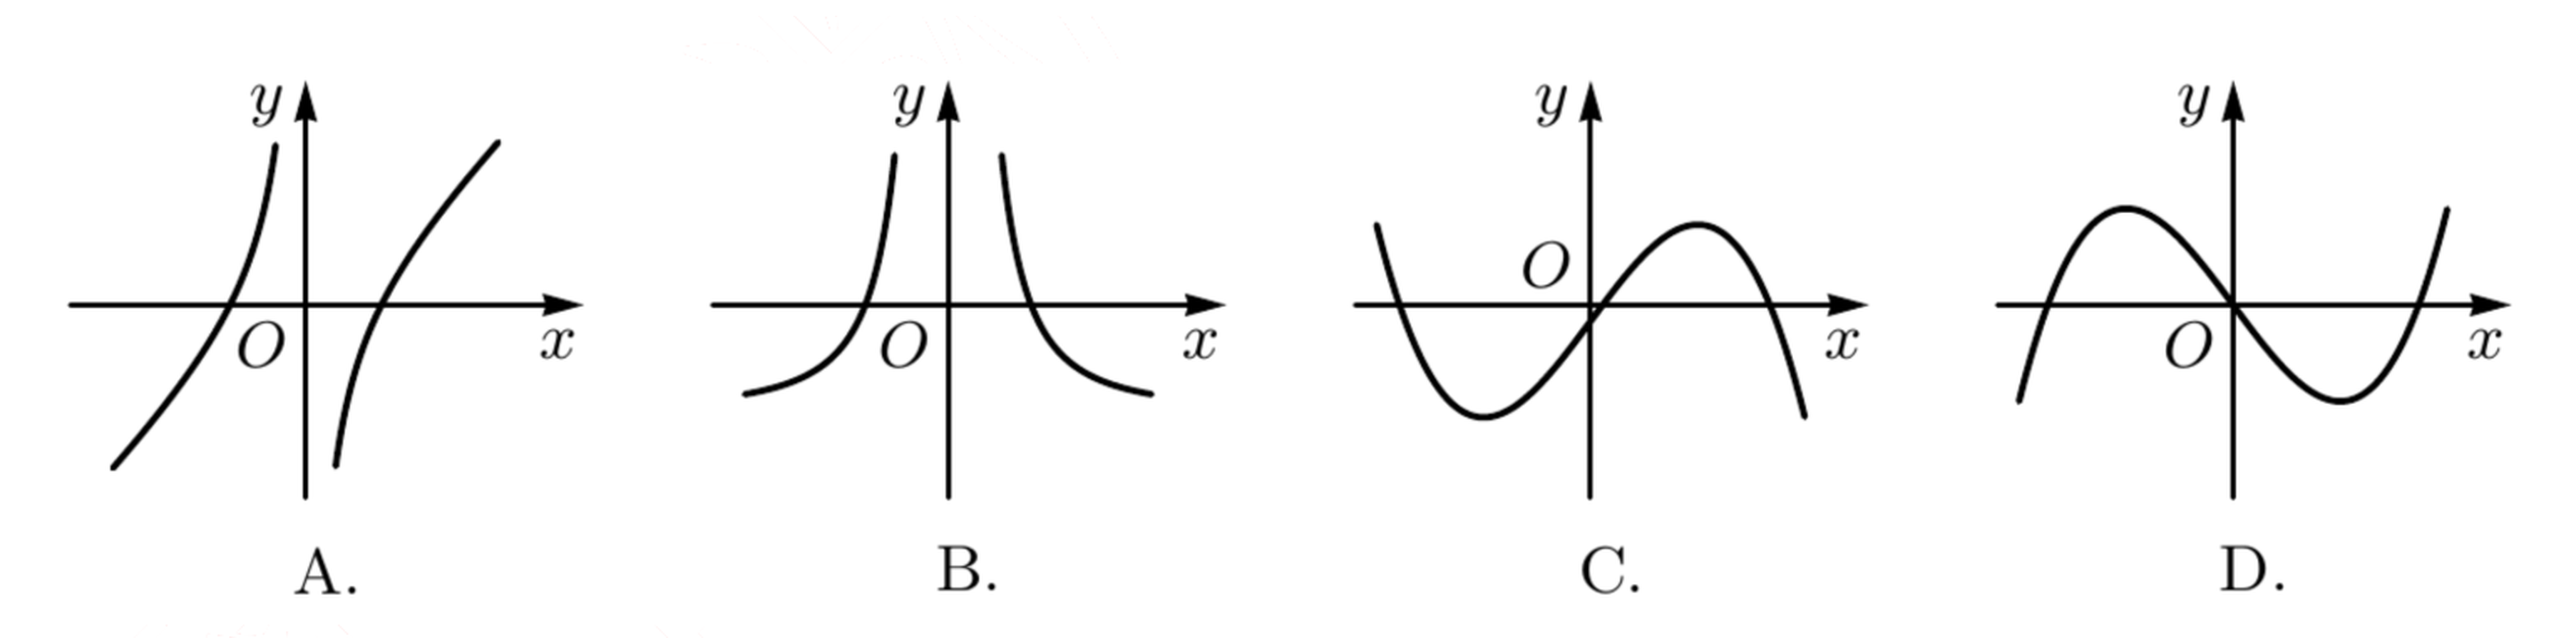
\includegraphics[width=0.90\textwidth]{figures/gao134_q13_options.png}
\end{center}

\ifanswer
\solbegin
\step{$f(x)$ 为偶函数，$g(x)$ 为奇函数，因此 $f(x)g(x)$ 为奇函数，排除 B.}
\step{又 $x=0$ 不在乘积函数的定义域内，其图象在 $y$ 轴上没有点，排除 C、D，}
\step{故选 $A$.}
\solend
\fi

\item 设全集为自然数集 $\N$，$E=\{x\mid x=2n,n\in\N\}$，$F=\{x\mid x=4n,n\in\N\}$，那么集合 $\N$ 可以表示成\mbox{（\quad）}

\keepwithprev
A. $E\cap F$\qquad\qquad B. $\overline{E}\cup F$\qquad\qquad C. $\overline{F}\cup E$\qquad\qquad D. $\overline{E}\cap\overline{F}$

\ifanswer
\solbegin
\step{$F\subseteq E$，所以 $\overline{F}\cup E=\N$，故选 $C$.}
\solend
\fi

\item 已知函数 $y=f(x)$，其中 $f(x)=x^2+bx$，则“$b<0$”是“$f(f(x))$ 的最小值与 $f(x)$ 的最小值相等”的\mbox{（\quad）}

\keepwithprev
A. 充分非必要条件\qquad\qquad B. 必要非充分条件

C. 充分必要条件\qquad\qquad D. 既非充分又非必要条件

\ifanswer
\solbegin
\step{$f(x)=\left(x+\dfrac b2\right)^2-\dfrac{b^2}4$，最小值为 $-\dfrac{b^2}4$，值域为 $\left[-\dfrac{b^2}4,+\infty\right)$.}
\step{当 $b<0$ 时，$-\dfrac b2>0\geqslant-\dfrac{b^2}4$，存在 $x$ 使 $f(x)=-\dfrac b2$，}
\step{从而 $f(f(x))$ 的最小值也为 $-\dfrac{b^2}4$，充分性成立.}
\step{当 $b=0$ 时，$f(x)=x^2$，$f(f(x))=x^4$，两者最小值均为 $0$，必要性不成立.}
\step{故选 $A$.}
\solend
\fi

\item 已知 $a,b,c\in\R$，若存在常数 $M>0$，使得 $a^2+b^2+c^2<M$，则称 $(a,b,c)$ 是有界数组. 对以下两个命题：

①若 $\lvert a^2+b+c\rvert+\lvert a^2+b-c\rvert\leqslant1$，则 $(a,b,c)$ 是有界数组；

②若 $\lvert a^2+b+c\rvert+\lvert a+b^2-c\rvert\leqslant1$，则 $(a,b,c)$ 是有界数组.% ②第二项为 \lvert a+b^2-c\rvert，与①刻意不同，照录

下列判断正确的是\mbox{（\quad）}

\keepwithprev
A. ①和②均为真命题\qquad\qquad B. ①和②均为假命题

C. ①为真命题，②为假命题\qquad D. ①为假命题，②为真命题

\ifanswer
\solbegin
\step{①取 $a=t,b=-t^2,c=0$，条件左端为 $0$，而 $a^2+b^2+c^2=t^2+t^4$ 可任意大，}
\step{故①为假命题.}
\step{②由条件，$a^2+a+b^2+b\leqslant\lvert a^2+b+c\rvert+\lvert a+b^2-c\rvert\leqslant1$.}
\step{由 $(a+1)^2+(b+1)^2\geqslant0$，得 $a^2+b^2\leqslant2(a^2+a+b^2+b)+2\leqslant4$.}
\step{又 $\lvert c\rvert\leqslant\lvert a^2+b+c\rvert+a^2+\lvert b\rvert\leqslant1+4+2=7$，故 $a^2+b^2+c^2\leqslant53<54$，}
\step{可取 $M=54$，故②为真命题.}
\step{故选 $D$.}
\solend
\fi

\end{enumerate}

\bigsec{三、解答题}

\begin{enumerate}
\setcounter{enumi}{16}

\item 已知不等式 $x^2-ax-b<0$ 的解集为 $A$，不等式 $\dfrac{3-2x}{x-1}<0$ 的解集为 $B$.

(1) 若 $a=5$，$b=-6$，求 $A\cap\overline{B}$；

(2) 若 $b=2a^2$，且 $A\cup B=B$，求实数 $a$ 的取值范围.

\ifanswer
\solbegin
\step{(1) 不等式 $\dfrac{3-2x}{x-1}<0$ 等价于 $x<1$ 或 $x>\dfrac32$，}
\step{所以 $B=(-\infty,1)\cup\left(\dfrac32,+\infty\right)$，$\overline{B}=\left[1,\dfrac32\right]$，}
\step{由 $x^2-5x+6=(x-2)(x-3)<0$，得 $A=(2,3)$，因此 $A\cap\overline{B}=\varnothing$.}
\step{(2) $A\cup B=B\Leftrightarrow A\subseteq B$，且 $x^2-ax-2a^2=(x-2a)(x+a)$，}
\step{当 $a=0$ 时，$A=\varnothing$，满足条件.}
\step{当 $a>0$ 时，$A=(-a,2a)$，$-a<0<1$，$A\subseteq B\Leftrightarrow2a\leqslant1$，得 $0<a\leqslant\dfrac12$.}
\step{当 $a<0$ 时，$A=(2a,-a)$，$2a<0<1$，$A\subseteq B\Leftrightarrow-a\leqslant1$，}
\step{得 $-1\leqslant a<0$.}
\step{因此 $a$ 的取值范围为 $\left[-1,\dfrac12\right]$.}
\solend
\fi

\item 为了在夏季降温和冬季供暖时减少能源损耗，房屋的屋顶和外墙需要建造隔热层. 某幢建筑物要建造可使用 $30$ 年的隔热层，每厘米厚的隔热层建造成本为 $9$ 万元. 该建筑物每年的能源消耗费用 $C$（万元）与隔热层厚度 $x$（cm）满足如下关系式：$C=\dfrac{k}{3x+5}$（$0\leqslant x\leqslant10$）. 若不建隔热层，每年能源消耗费用为 $8$ 万元. 设 $y$（万元）为隔热层建造费用与 $30$ 年的能源消耗费用之和.

(1) 求 $k$ 的值及 $y$ 的表达式；

(2) 隔热层修建多厚时，总费用 $y$ 最小？并求最小值.

\ifanswer
\solbegin
\step{(1) 不建隔热层时 $x=0$，$C=8$，所以 $\dfrac k5=8$，得 $k=40$.}
\step{隔热层建造费用为 $9x$ 万元，$30$ 年的能源消耗费用为 $30\times\dfrac{40}{3x+5}$ 万元.}
\step{因此 $y=9x+\dfrac{1200}{3x+5}$，$0\leqslant x\leqslant10$.}
\step{(2) 令 $t=3x+5$，则 $5\leqslant t\leqslant35$，且 $y=3t+\dfrac{1200}{t}-15$，}
\step{因为 $t>0$，由基本不等式得 $y\geqslant2\sqrt{3t\cdot\dfrac{1200}{t}}-15=105$，}
\step{当且仅当 $3t=\dfrac{1200}{t}$，即 $t=20$时取等号，此时 $x=5\in[0,10]$，}% 原卷"20"与"时"之间未留空，照录
\step{所以隔热层厚度为 $5$ cm 时，总费用最小，最小值为 $105$ 万元.}
\solend
\fi

\item 已知 $f(x)=ax^2+\dfrac1x$，其中 $a$ 为常数.

(1) 若 $a\in(1,3)$，判断函数 $y=f(x)$ 在 $[1,2]$ 上的单调性，并用定义证明；

(2) 求函数 $y=f(x)-x-\dfrac1x$ 在 $[1,2]$ 上的最大值 $g(a)$.

\ifanswer
\solbegin
\step{(1) 任取 $x_1,x_2\in[1,2]$，且 $x_1<x_2$，}
\step{则 $f(x_2)-f(x_1)=(x_2-x_1)\left[a(x_1+x_2)-\dfrac1{x_1x_2}\right]$，}
\step{由 $a>1$，$x_1+x_2\geqslant2$，$x_1x_2\geqslant1$，得 $a(x_1+x_2)-\dfrac1{x_1x_2}>2-1>0$，}
\step{因此 $f(x_2)>f(x_1)$，$f(x)$ 在 $[1,2]$ 上为严格增函数.}
\step{(2) 令 $h(x)=f(x)-x-\dfrac1x=ax^2-x$，其中 $x\in[1,2]$.}
\step{若 $a=0$，则 $h(x)=-x$，所以 $h(x)_{max}=h(1)=-1$；}
\step{若 $a<0$，二次函数的图象的对称轴为 $x=\dfrac1{2a}<0$，}
\step{所以 $y=h(x)$ 在 $[1,2]$ 上是严格减函数，所以 $h(x)_{max}=h(1)=a-1$；}
\step{若 $a>0$ 且 $\dfrac1{2a}>\dfrac32$，即 $0<a<\dfrac13$ 时，$h(x)_{max}=h(1)=a-1$.}
\step{若 $a>0$ 且 $\dfrac1{2a}\leqslant\dfrac32$，即 $a\geqslant\dfrac13$ 时，$h(x)_{max}=h(2)=4a-2$.}
\step{综上所述，$g(a)=\begin{cases}a-1,a<\dfrac13\\4a-2,a\geqslant\dfrac13\end{cases}$.}
\solend
\fi

\item 已知 $f(x)=\dfrac{ax^2+1}{bx+c}$（$a,b,c\in\Z$）.

(1) 若函数 $y=f(x)$ 是奇函数，且 $f(1)=2$，$f(2)<3$，求 $a,b,c$ 的值；

(2) 若函数 $y=f(x)$ 是偶函数，且 $ac<0$，$f(2a^2+a+1)<f(-3a^2+2a-1)$，求 $a$ 的值；

(3) 若 $b=a+c^2$，且满足不等式 $\lvert f(x)\rvert\geqslant1$ 的 $x$ 的最大值为 $0$，求 $c$ 的值.

\ifanswer
\solbegin
\step{(1) 由 $f(-x)=-f(x)$，交叉相乘得 $2c(ax^2+1)=0$ 恒成立，}
\step{因此 $c=0$，$b\neq0$.}
\step{由 $f(1)=2$，得 $a+1=2b$，}
\step{于是 $f(2)=\dfrac{4a+1}{2b}=4-\dfrac3{2b}<3\Leftrightarrow0<b<\dfrac32$，}
\step{因为 $b\in\Z$，所以 $b=1$，进而 $a=1$，$c=0$.}
\step{(2) 由 $f(-x)=f(x)$，交叉相乘得 $2bx(ax^2+1)=0$ 恒成立，因此 $b=0$.}
\step{此时 $f(x)=\dfrac ac x^2+\dfrac1c$，且 $\dfrac ac<0$.}
\step{设 $u=2a^2+a+1$，$v=-3a^2+2a-1$.}
\step{方程 $2a^2+a+1=0$ 与 $3a^2-2a+1=0$ 的判别式分别为 $-7$ 与 $-8$，}
\step{都小于 $0$，所以 $u>0$，$v<0$.}
\step{于是 $f(u)<f(v)\Leftrightarrow u^2>v^2\Leftrightarrow u>-v\Leftrightarrow-a^2+3a>0\Leftrightarrow0<a<3$，}
\step{因为 $a\in\Z$，所以 $a=1$ 或 $a=2$.}
\step{(3) 因为解集的最大值为 $0$，所以 $f(0)$ 有定义且 $\lvert f(0)\rvert\geqslant1$，}
\step{即 $c\neq0$，$\left\lvert\dfrac1c\right\rvert\geqslant1$，结合 $c\in\Z$，得 $c=\pm1$，从而 $b=a+1$.}
\step{当 $x=2$ 时，分母 $2a+2+c$ 为奇数，必不为 $0$；}
\step{又因为 $2>0$，必须有 $\lvert f(2)\rvert<1\Leftrightarrow\lvert4a+1\rvert<\lvert2a+2+c\rvert$，}
\step{若 $c=-1$，则 $(4a+1)^2<(2a+1)^2\Leftrightarrow4a(3a+1)<0\Leftrightarrow-\dfrac13<a<0$，}
\step{不存在满足条件的整数 $a$.}
\step{若 $c=1$，则 $(4a+1)^2<(2a+3)^2\Leftrightarrow4(3a+2)(a-1)<0\Leftrightarrow-\dfrac23<a<1$，}
\step{所以 $a=0$，$b=1$，此时 $f(x)=\dfrac1{x+1}$，}
\step{且 $\lvert f(x)\rvert\geqslant1\Leftrightarrow0<\lvert x+1\rvert\leqslant1\Leftrightarrow x\in[-2,-1)\cup(-1,0]$，}
\step{解集的最大值确为 $0$，因此 $c=1$.}
\solend
\fi

\item 已知函数 $y=f(x)$ 的定义域为 $\R$，且当 $x>0$ 时，$f(x)=\dfrac1{x+1}$. 对任意 $x_0\in\R$，定义集合 $D(x_0)=\{d\mid f(x_0+d)>f(x_0)\}$.

(1) 若当 $x\leqslant0$ 时，$f(x)=-2x+1$，求函数 $y=f(x)$ 的值域；

(2) 若 $y=f(x)$ 是偶函数，且 $f(0)=1$，求证：$D(-2)=\{-d\mid d\in D(2)\}$；

(3) 若 $y=f(x)$ 是奇函数，且 $x_1x_2\neq0$，求证：“$f(x_1)\leqslant f(x_2)$”的充要条件是\!\mbox{“$D(x_2)\subseteq D(x_1)$”}.

\ifanswer
\solbegin
\step{(1) 当 $x>0$ 时，$0<f(x)<1$；当 $x\leqslant0$ 时，$f(x)=-2x+1\geqslant1$.}
\step{函数的值域为 $(0,1)\cup[1,+\infty)=(0,+\infty)$.}
\step{(2) 由 $f(x)$ 是偶函数及 $f(0)=1$，得 $f(x)=\dfrac1{1+\lvert x\rvert}$，且 $f(2)=f(-2)=\dfrac13$.}
\stepm{法一：}{$D(2)=\left\{d\mid\dfrac1{1+\lvert2+d\rvert}>\dfrac13\right\}=\{d\mid\lvert2+d\rvert<2\}=(-4,0)$，}
\step{$D(-2)=\left\{d\mid\dfrac1{1+\lvert-2+d\rvert}>\dfrac13\right\}=\{d\mid\lvert-2+d\rvert<2\}=(0,4)$，}
\step{因此 $\{-d\mid d\in D(2)\}=(0,4)=D(-2)$.}
\stepm{法二：}{任取 $d\in D(-2)$，由定义得 $f(-2+d)>f(-2)$.}
\step{因为 $y=f(x)$ 是偶函数，所以对任意的实数 $x$，有 $f(-x)=f(x)$，}
\step{因此 $f(-2+d)=f(-(-2+d))=f(2-d)$，且 $f(-2)=f(2)$.}
\step{所以不等式 $f(-2+d)>f(-2)$ 等价于 $f(2-d)>f(2)$，}
\step{这恰好是 $-d\in D(2)$ 的定义，}
\step{所以 $d\in D(-2)\Leftrightarrow-d\in D(2)$，故 $D(-2)=\{-d\mid d\in D(2)\}$.}
\step{(3) 由 $f(x)$ 是奇函数，得 $f(0)=0$；}
\step{当 $x<0$ 时，$f(x)=-f(-x)=-\dfrac1{1-x}=\dfrac1{x-1}$；}
\step{所以 $f(x)=\begin{cases}\dfrac1{x-1},&x<0\\0,&x=0;\\\dfrac1{x+1},&x>0\end{cases}$}
% 2026-11-15 回原图订正：原卷 11 页此 cases 块末无句点，本稿初转顺手补了西文句点，今删去（Q19 08 页同类块末有句点，照录保留）。
\step{当 $x_0<0$ 时，$D(x_0)=\{d\mid f(x_0+d)>f(x_0)\}=(-\infty,0)\cup[-x_0,+\infty)$，}
\step{当 $x_0=0$ 时，$D(0)=\{d\mid f(0+d)>f(0)\}=(0,+\infty)$，}
\step{当 $x_0>0$ 时，$D(x_0)=\{d\mid f(x_0+d)>f(x_0)\}=(-x_0,0)$.}
\stepm{先证明必要性.}{若 $f(x_1)\leqslant f(x_2)$，仅需讨论三类情形：}
\step{若 $x_2\leqslant x_1<0$，}
\step{则 $D(x_1)=(-\infty,0)\cup[-x_1,+\infty),D(x_2)=(-\infty,0)\cup[-x_2,+\infty)$，}
\step{故 $D(x_2)\subseteq D(x_1)$；}
\step{若 $0<x_2\leqslant x_1$，则 $D(x_1)=(-x_1,0),D(x_2)=(-x_2,0)$，}
\step{故 $D(x_2)\subseteq D(x_1)$；}
\step{若 $x_1<0<x_2$，则 $D(x_1)=(-\infty,0)\cup[-x_1,+\infty),D(x_2)=(-x_2,0)$，}
\step{故 $D(x_2)\subseteq D(x_1)$.}
\stepm{再证明充分性.}{若 $D(x_2)\subseteq D(x_1)$，}
\step{若 $x_1<0,x_2<0$，}
\step{则 $D(x_1)=(-\infty,0)\cup[-x_1,+\infty),D(x_2)=(-\infty,0)\cup[-x_2,+\infty)$，}
\step{由 $D(x_2)\subseteq D(x_1)$ 得 $x_2\leqslant x_1$，}
\step{又 $y=f(x)$ 在 $(-\infty,0)$ 上是严格减函数，所以 $f(x_1)\leqslant f(x_2)$；}
\step{若 $x_1>0,x_2>0$，则 $D(x_1)=(-x_1,0),D(x_2)=(-x_2,0)$，}
\step{由 $D(x_2)\subseteq D(x_1)$ 得 $x_2\leqslant x_1$，}
\step{又 $y=f(x)$ 在 $(0,+\infty)$ 上是严格减函数，所以 $f(x_1)\leqslant f(x_2)$；}
\step{若 $x_1<0,x_2>0$，则 $f(x_1)<0<f(x_2)$，结论成立；}
\step{若 $x_1>0,x_2<0$，此时 $D(x_1)=(-x_1,0)$ 中只有负数，}
\step{而 $D(x_2)=(-\infty,0)\cup[-x_2,+\infty)$ 中有正数，$D(x_2)\subseteq D(x_1)$ 不成立.}
\step{综上，“$f(x_1)\leqslant f(x_2)$”的充要条件是“$D(x_2)\subseteq D(x_1)$”.}
\solend
\fi

\end{enumerate}

\end{document}
"
%
% ① 原始材料：微信公众号"魔都数学加油站"文章，作者破晓，2026-11-15 18:04 发布；
% 连载"27学年高一134"，原文标题"27学年高一134——2026-2027年上海市华师大二附中高一上期中"；
% 原文链接：https://mp.weixin.qq.com/s/bQlkmlGdCtAlytY331vf3g。
% 正文为 13 张 PNG 页（01、04、06、08、09、10、11、12、13 为 2560x3620；
% 02、03、05、07 为 4762x6735，同一篇各页分辨率不同，逐页按各自分辨率裁图核对），
% 题目下印有【解析】，为讲评版。题目、解析均据原图转录；卷面粉红色水印
% "魔都数学加油站"及公众号页脚未录入。
% 全卷 2 幅插图，均在第 04 页：第 13 题题干 y=f(x)、y=g(x) 两幅函数图象合并裁为
% figures/gao134_q13_graphs.png，第 13 题 A/B/C/D 四幅函数图象选项合并裁为
% figures/gao134_q13_options.png；两图均取原卷 04 页截图 3× LANCZOS 放大、
% 白化粉色水印（只白化浅粉色 R>175 且 G>140 且 B>140 的像素，保留红色标签）。
% 注意：本卷 Q13 四幅选项在原卷排为"一行四幅"（1×4），并非 高一132 第 14 题
% 的 2×2 排布，本稿按原卷 1×4 合并裁为一张，不重排、不用 TikZ 重绘。
%
% 卷首标题：原卷印作"2026-2027 年华师大二附中高一上期中"（公众号标题中的"上海市"
% 卷面标题行没有，本稿照卷面），年份区间按全稿惯例排 en dash；原卷未印副标题，
% 本卷为期中卷、跨集合与常用逻辑用语／不等式／函数三章，按题目内容标为
% "集合与常用逻辑用语、不等式、函数"（与 125／126／128／129／131／132／133 同期中卷口径相同）：
% 集合与逻辑见 Q6、Q10、Q14、Q16、Q17、Q21，不等式见 Q3、Q7、Q9、Q11、Q15、Q18、Q19，
% 函数（函数性质、二分法、奇偶性、基本不等式应用）见 Q4、Q5、Q8、Q12、Q13、Q20。
%
% 题号体例：本卷共 19 题——一、填空题 3—12（10 题）、二、选择题 13—16（4 题）、
% 三、解答题 17—21（5 题）。三节分别 \setcounter{enumi}{2}／{12}／{16}。
% 第 13 页仅为 Q21 (3) 解析续尾，全卷无「四、附加题」。
%
% ② 与原卷的排版差异：
%   ① 原文从第 3 题起，本稿保留原题号（见上"题号体例"）；
%   ② 原卷每题下直接印【解析】，本稿按全稿惯例置于答案版；第 13—16 题答案均在
%      解析末句"故选 …"，题干括号内留空、不另提 \ans{}（四题均无独立答案段）；
%      全卷无只印括号内答案、无解析的选择题；
%   ③ 原卷未印副标题，本稿按"知识模块"口径补出；
%   ④ 原卷填空横线按全稿惯例排为 \blankline[4.4em]；选择题括号排 \mbox{（\quad）}、
%      每个选项段前按惯例加 \keepwithprev（Q13 四选项为图，守卫前行为 \begin{center}；
%      Q15、Q16 四选项分两行排，\keepwithprev 只加在 A. 行前）；解答题不留作答区、
%      不加 \anspace（原卷为讲评版，与 129／131／132／133 同）；
%   ⑤ 原卷数集印黑板粗体（Q7／Q11／Q12／Q16／Q21 的 R、Q14／Q20 的 N、Q20 的 Z），
%      按全稿惯例统一排 \R／\N／\Z；绝对值排 \lvert…\rvert，集合描述竖线排 \mid；不等号按全稿惯例排
%      \leqslant／\geqslant；补集照原卷上划线排 \overline{B}、\overline{E}、\overline{F}；
%   ⑥ 子题标号 (1)(2)(3) 与括注原卷均用半角括号，照录（与 131／132／133 同）；
%      圈数字 ①② 照录；原卷 Q21 (2) 解析"法一：""法二："与 Q21 (3) 解析
%      "先证明必要性.""再证明充分性."四处标签印红色加粗，按 高一53／108／133 成例排
%      \stepm{法一：}／\stepm{法二：}／\stepm{先证明必要性.}／\stepm{再证明充分性.}
%      （加粗着色、不引入红色，不动 common.sty）；Q8 解析"第 1 步：""第 2 步：""
%      "第 3 步："原卷印黑色常规宋体（非红非粗），照录为普通 \step 行内文字；
%   ⑦ 数学式内半角逗号照录（如 Q6 $A=\{0,1,2,3\}$、Q14 $x=2n,n\in\N$、
%      Q16 $a,b,c\in\R$ 与 $a=t,b=-t^2,c=0$、Q19 $x_1,x_2\in[1,2]$、
%      Q20 $a,b,c\in\Z$、Q21 $x_1<0,x_2<0$ 与 $D(x_1)=(-x_1,0),D(x_2)=(-x_2,0)$）；
%      原卷行末全角句点按全稿惯例从宽排西文句点；cases 块末的句点逐处照录：
%      Q19 解析（08 页）块末原卷有句点照录、Q21 (3) 解析（11 页）块末原卷无句点不补，
%      两处原卷自身不统一（2026-11-15 回原图核对，本稿初转曾顺手补句点，已删去）；
%   ⑧ 原卷 Q8 解析跨 01—02 页、Q10 解析跨 02—03 页、Q12 解析跨 03—04 页、
%      Q16 解析跨 05—06 页、Q17 解析跨 06—07 页、Q20 解析跨 08—10 页、
%      Q21 解析跨 10—13 页，本稿按题合并连续排版；末页第 13 页为
%      Q21 (3) 解析续尾与"综上"一句，按实际印刷行单列；
%   ⑨ 题干中的中文弯引号按原卷照录（Q10 研究问题、Q15 条件、Q21 (3) 充要条件），
%      注释内一律 ASCII 引号。
%
% 判别式字形：全卷仅 Q9 解析末行出现一处判别式记号
%   "两值均满足 $\Delta=p^2-4p=18\mp12\sqrt2>0$"，逐处放大核对，原卷印高三角
%   $\Delta$（等腰、高，实测高宽比约 1.14），照录 \Delta；卷内无扁三角 \triangle，
%   与 高一132 同题排 $\triangle$、高一133 部分判别式排 $\triangle$ 均不同。
%
% 子集符号：Q6 题干 $C\subseteq A$、$C\subseteq B$ 与解析 $C\subseteq A\cap B$、
%   Q14 解析 $F\subseteq E$、Q17 解析 $A\subseteq B$、Q21 题干与解析各处的
%   $D(x_2)\subseteq D(x_1)$，全部印带下划线的 $\subseteq$，逐处放大核对，
%   照录 \subseteq；全卷未出现单线 \subset。
%
% 原卷存疑照录（均照录未改，正文对应处另有 % 注）：
%   第 6 题题干集合 $A=\{0,1,2,3\}$ 三个逗号后不留空，紧邻的 $B=\{0,2,4,5\}$
%      三个逗号后却留空，同卷同一行两集合排字不一，照录其逗号均为半角；
%   第 16 题命题②作 $\lvert a^2+b+c\rvert+\lvert a+b^2-c\rvert\leqslant1$，
%      与命题①第二项 $\lvert a^2+b-c\rvert$ 不同（①无 $b$ 的平方、②有），
%      两命题刻意不同，照录；解析"②由条件，$a^2+a+b^2+b\leqslant\cdots$"
%      由两项相加直接得到，照录；
%   第 18 题 (2) 解析"即 $t=20$时取等号"中"20"与"时"之间原卷未留空，照录；
%   第 19 题解析 $h(x)_{max}$ 的"max"下标三处字形不一（斜体／正体混排），照录；
%   第 20 题 (1)(2) 解析"由 $f(-x)=-f(x)$，交叉相乘得……"与"由 $f(-x)=f(x)$，
%      交叉相乘得……"两处措辞照录；
%   第 21 题 (2) 原卷并存"法一"（集合计算）与"法二"（定义推证）两套证明，照录不删。
%
% 行数复核：逐题数 \step/\stepm 条数，合计 134 条（Q3：2；Q4：1；Q5：1；Q6：1；
% Q7：2；Q8：4；Q9：3；Q10：4；Q11：5；Q12：8；Q13：3；Q14：1；Q15：5；
% Q16：7；Q17：9；Q18：7；Q19：11；Q20：22；Q21：38），与原卷印刷行逐题相等
% （cases 块作一个印刷行计）。第 13—16 题答案在解析末句，括号内留空、不另提 \ans{}；
% 第 21 题四条 \stepm 计入 38 条内。
%
\documentclass[a4paper,11pt]{article}
\usepackage{common}

\begin{document}

\examtitlest[3]{2026--2027 年华师大二附中高一上期中}{集合与常用逻辑用语、不等式、函数}

\bigsec{一、填空题}

\begin{enumerate}
\setcounter{enumi}{2}

\item 不等式 $\lvert 2x+1\rvert\geqslant3$ 的解集为\blankline[4.4em].

\ifanswer
\solbegin
\step{$\lvert 2x+1\rvert\geqslant3\Leftrightarrow 2x+1\leqslant-3$ 或 $2x+1\geqslant3\Leftrightarrow x\leqslant-2$ 或 $x\geqslant1$，}
\step{故解集为 $(-\infty,-2]\cup[1,+\infty)$.}
\solend
\fi

\item 函数 $y=\sqrt{x+1}+\dfrac1x$ 的定义域为\blankline[4.4em].

\ifanswer
\solbegin
\step{$x+1\geqslant0$ 且 $x\neq0$，得定义域为 $[-1,0)\cup(0,+\infty)$.}
\solend
\fi

\item 已知等式 $3x^2-4x-2=a(x-1)^2+b(x-1)+c$ 恒成立，其中 $a$、$b$、$c$ 为常数，则 $a-b+c=$\blankline[4.4em].

\ifanswer
\solbegin
\step{令 $x=0$，得 $a-b+c=-2$.}
\solend
\fi

\item 已知集合 $A=\{0,1,2,3\}$，$B=\{0,2,4,5\}$，$C\subseteq A$，$C\subseteq B$，符合条件的集合 $C$ 有\blankline[4.4em]个.% 原卷 A 的逗号后不留空、B 的逗号后留空，排字不一，照录

\ifanswer
\solbegin
\step{$C\subseteq A\cap B=\{0,2\}$，所以符合条件的集合 $C$ 有 $2^2=4$ 个.}
\solend
\fi

\item 设 $a$、$b\in\R$，且 $a^2+4b^2=2$，则 $ab$ 的最大值为\blankline[4.4em].

\ifanswer
\solbegin
\step{$(a-2b)^2=a^2+4b^2-4ab=2-4ab\geqslant0$，得 $ab\leqslant\dfrac12$，}
\step{当且仅当 $a=2b=\pm1$ 时取等号，故 $ab$ 的最大值为 $\dfrac12$.}
\solend
\fi

\item 已知函数 $y=x(13-2x)^2-140$，用二分法求函数在区间 $(3,4)$ 上的零点时，第 3 步应计算 $x=$\blankline[4.4em]的函数值.

\ifanswer
\solbegin
\step{记 $f(x)=x(13-2x)^2-140$，则 $f(3)=7>0$，$f(4)=-40<0$.}
\step{第 1 步：$f\left(\dfrac72\right)=-14<0$，区间缩小为 $\left(3,\dfrac72\right)$.}
\step{第 2 步：$f\left(\dfrac{13}4\right)=-\dfrac{43}{16}<0$，区间缩小为 $\left(3,\dfrac{13}4\right)$.}
\step{第 3 步：应计算 $x=\dfrac{3+\frac{13}4}2=\dfrac{25}8$ 的函数值.}
\solend
\fi

\item 已知一元二次方程 $x^2+px+p=0$ 的两个实根分别为 $x_1$、$x_2$，且 $x_1^2x_2+x_2^2x_1=-18$，则 $p=$\blankline[4.4em].% 判别式 \Delta 高三角，逐处放大核对

\ifanswer
\solbegin
\step{由韦达定理，$x_1+x_2=-p$，$x_1x_2=p$，}
\step{则 $x_1^2x_2+x_2^2x_1=x_1x_2(x_1+x_2)=-p^2=-18\Rightarrow p=\pm3\sqrt2$，}
\step{两值均满足 $\Delta=p^2-4p=18\mp12\sqrt2>0$，故 $p=\pm3\sqrt2$.}
\solend
\fi

\item 研究问题：“已知关于 $x$ 的不等式 $ax^2-bx+c>0$ 的解集为 $(1,2)$，解关于 $x$ 的不等式 $cx^2-bx+a>0$”，有如下解法：

解：由 $ax^2-bx+c>0\Rightarrow a-b\left(\dfrac1x\right)+c\left(\dfrac1x\right)^2>0$，令 $y=\dfrac1x$，则 $y\in\left(\dfrac12,1\right)$，

所以不等式 $cx^2-bx+a>0$ 的解集为 $\left(\dfrac12,1\right)$.

参考上述解法，已知关于 $x$ 的不等式 $\dfrac{k}{x+a}+\dfrac{x+b}{x+c}<0$ 的解集为 $(-3,-1)\cup(2,4)$，则关于 $x$ 的不等式 $\dfrac{kx}{ax-1}+\dfrac{bx-1}{cx-1}<0$ 的解集为\blankline[4.4em].

\ifanswer
\solbegin
\step{当 $x=0$ 时，所求不等式左端为 $1$，不满足不等式.}
\step{当 $x\neq0$ 时，两个分式的分子、分母同除以 $x$，得 $\dfrac{k}{a-\frac1x}+\dfrac{b-\frac1x}{c-\frac1x}<0$.}
\step{令 $t=-\dfrac1x$，则所求不等式化为 $\dfrac{k}{t+a}+\dfrac{t+b}{t+c}<0$，即 $-\dfrac1x\in(-3,-1)\cup(2,4)$，}
\step{解得 $x\in\left(-\dfrac12,-\dfrac14\right)\cup\left(\dfrac13,1\right)$.}
\solend
\fi

\item 已知 $a\in(0,+\infty)$，若对任意的 $x\in(0,+\infty)$，均有 $\lvert x^2-a\rvert+\lvert x+b\rvert=\lvert x^2+x-a+b\rvert$，则 $a^2-b^2$ 的最小值为\blankline[4.4em].

\ifanswer
\solbegin
\step{原等式成立的充要条件是 $(x^2-a)(x+b)\geqslant0$.}
\step{当 $0<x<\sqrt a$ 时须有 $x+b\leqslant0$；当 $x>\sqrt a$ 时须有 $x+b\geqslant0$，因此 $b=-\sqrt a$.}
\step{此时 $(x^2-a)(x+b)=(x+\sqrt a)(x-\sqrt a)^2\geqslant0$，满足题意.}
\step{$a^2-b^2=a^2-a=\left(a-\dfrac12\right)^2-\dfrac14\geqslant-\dfrac14$，}
\step{当 $a=\dfrac12$，$b=-\dfrac{\sqrt2}2$ 时取等号，最小值为 $-\dfrac14$.}
\solend
\fi

\item 已知函数 $y=f(x)$ 在 $\R$ 上是严格增函数，当 $x\neq0$ 且 $f(x)\neq0$ 时，满足 $f(x)\cdot f\left[\dfrac1{f(x)}+\dfrac1x\right]=1$，则 $f(1)=$\blankline[4.4em].

\ifanswer
\solbegin
\step{当 $xf(x)>0$ 时，记 $t=\dfrac1{f(x)}+\dfrac1x\neq0$，则 $f(t)=\dfrac1{f(x)}\neq0$.}
\step{将 $t$ 代入题设，得 $f\left(f(x)+\dfrac1t\right)=f(x)$，严格增性给出 $f(x)+\dfrac1t=x$，}
\step{化简得 $f(x)^2+xf(x)-x^2=0$，由 $\dfrac{f(x)}x>0$ 得 $f(x)=\dfrac{\sqrt5-1}2x$.}
\step{设 $a=f(0)$，若 $a>0$，则 $f(a)>f(0)=a>0$；}
\step{若 $a<0$，则 $f(a)<f(0)=a<0$.}
\step{两种情形都有 $af(a)>0$ 且 $\dfrac{f(a)}a>1$，与上式 $\dfrac{f(a)}a=\dfrac{\sqrt5-1}2<1$ 矛盾，}
\step{因此 $f(0)=0$.}
\step{于是 $f(1)>0$，代入上式得 $f(1)=\dfrac{\sqrt5-1}2$.}
\solend
\fi

\end{enumerate}

% 第 13 题是"节标题 + 题干 + 两幅图 + 四幅选项图"约 15cm 的整块，
% 守卫只放在 \bigsec 之前；若再在 \item 之前放第二枚，会在标题已印出后才触发换页，
% 把题目推走、留下孤立节标题（切页审计 B 类）。高度须覆盖整块。
\needvspace{16cm}
\bigsec{二、选择题}

\begin{enumerate}
\setcounter{enumi}{12}

\item 已知函数 $y=f(x)$ 与 $y=g(x)$ 的图象如图所示，则函数 $y=f(x)\cdot g(x)$ 的图象可能是\mbox{（\quad）}

\keepwithprev
\begin{center}
% 题干 y=f(x)、y=g(x) 两幅函数图象取原卷 04 页截图去粉色水印，按原卷左右排布合并为一张
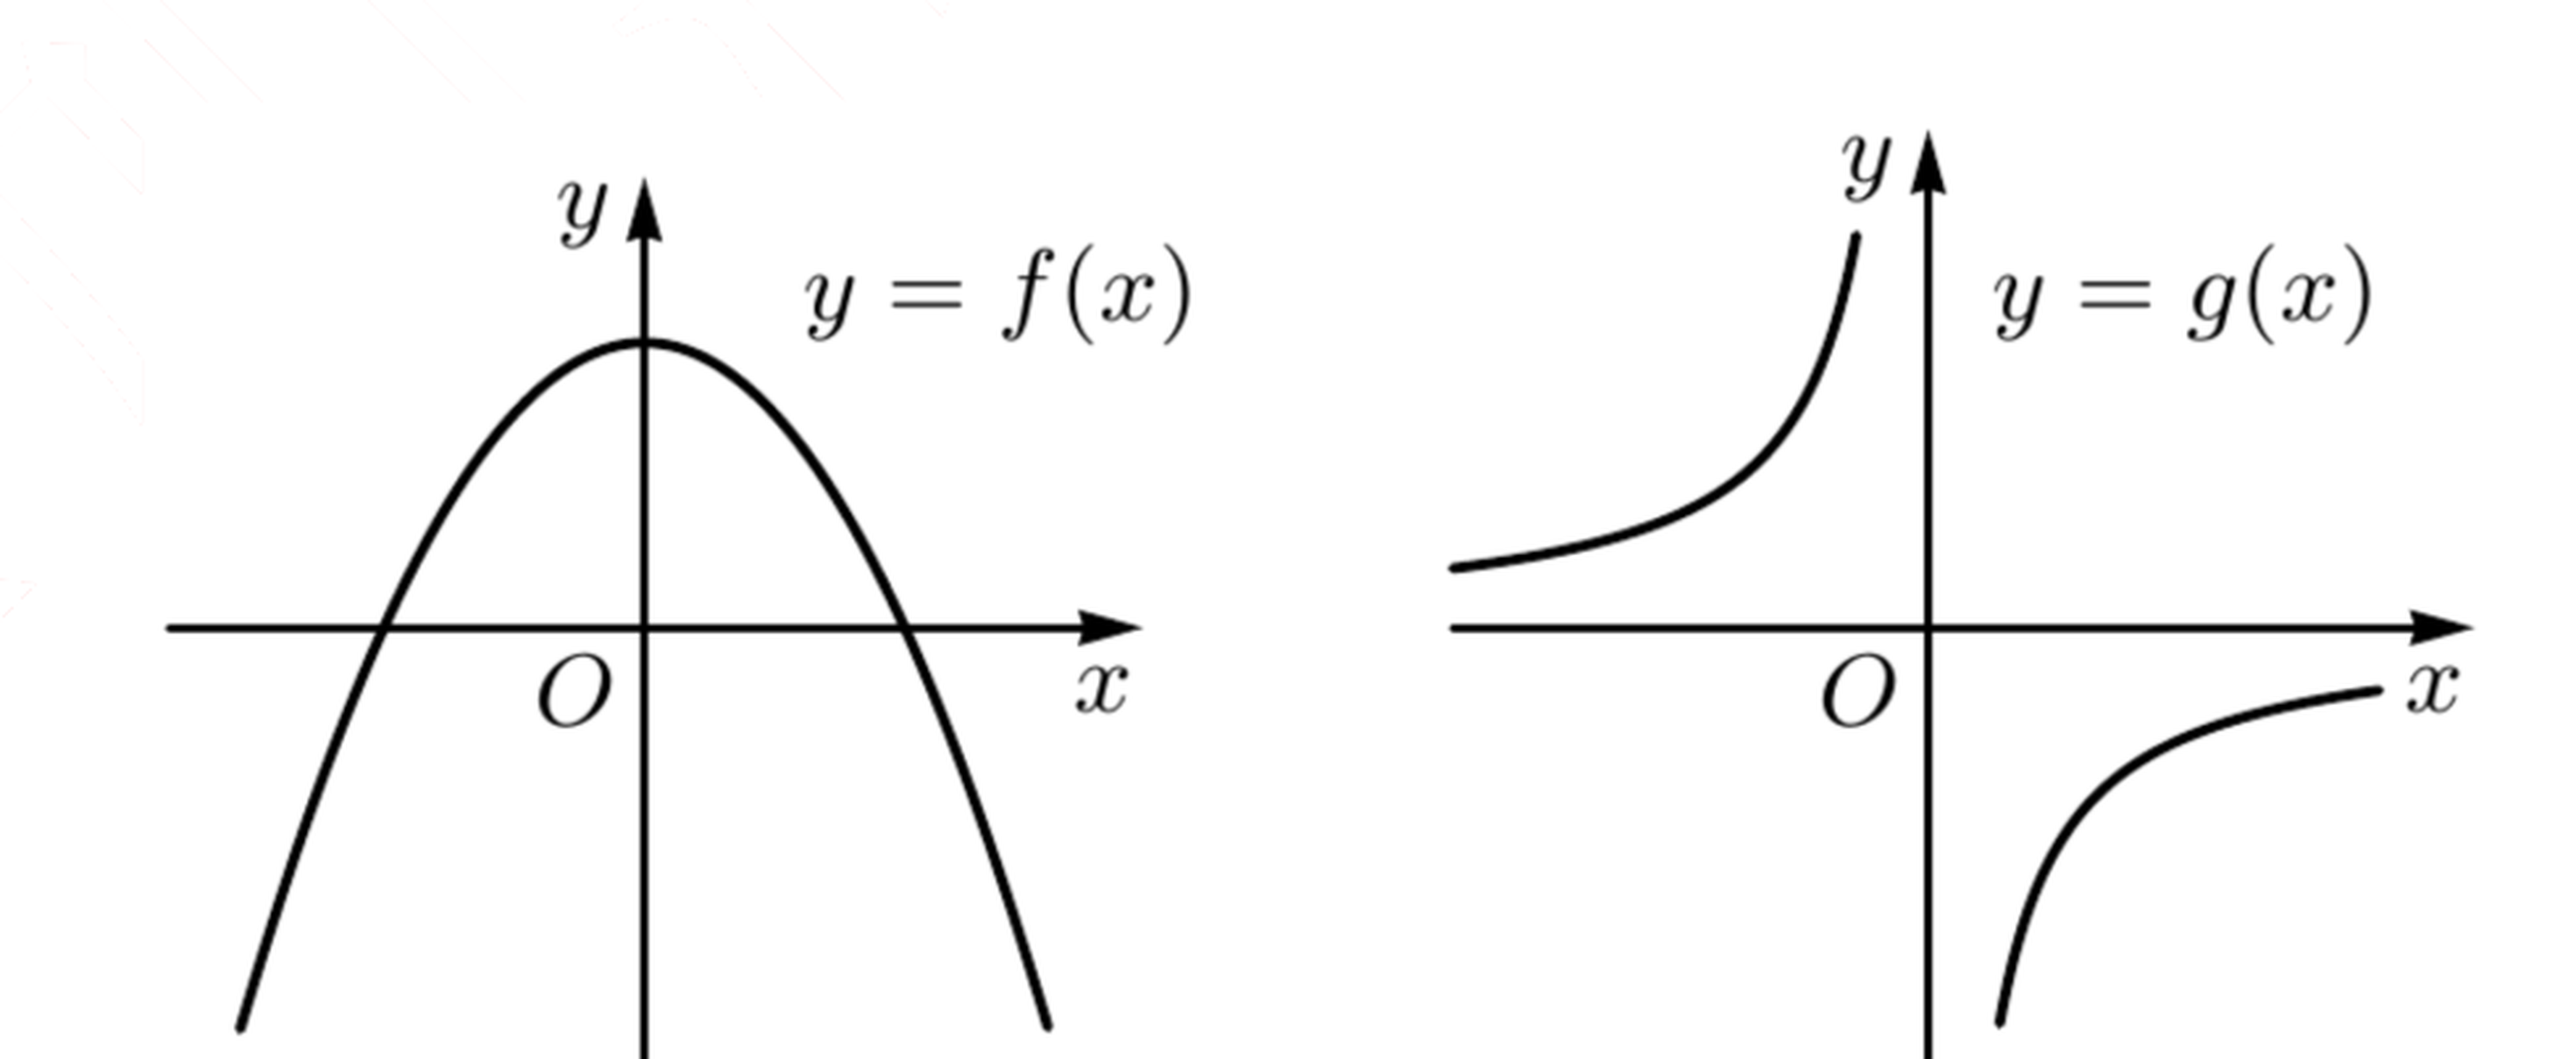
\includegraphics[width=0.72\textwidth]{figures/gao134_q13_graphs.png}\\[0.6em]
% A/B/C/D 四幅函数图象选项取原卷 04 页截图去粉色水印，按原卷一行四幅排布合并为一张
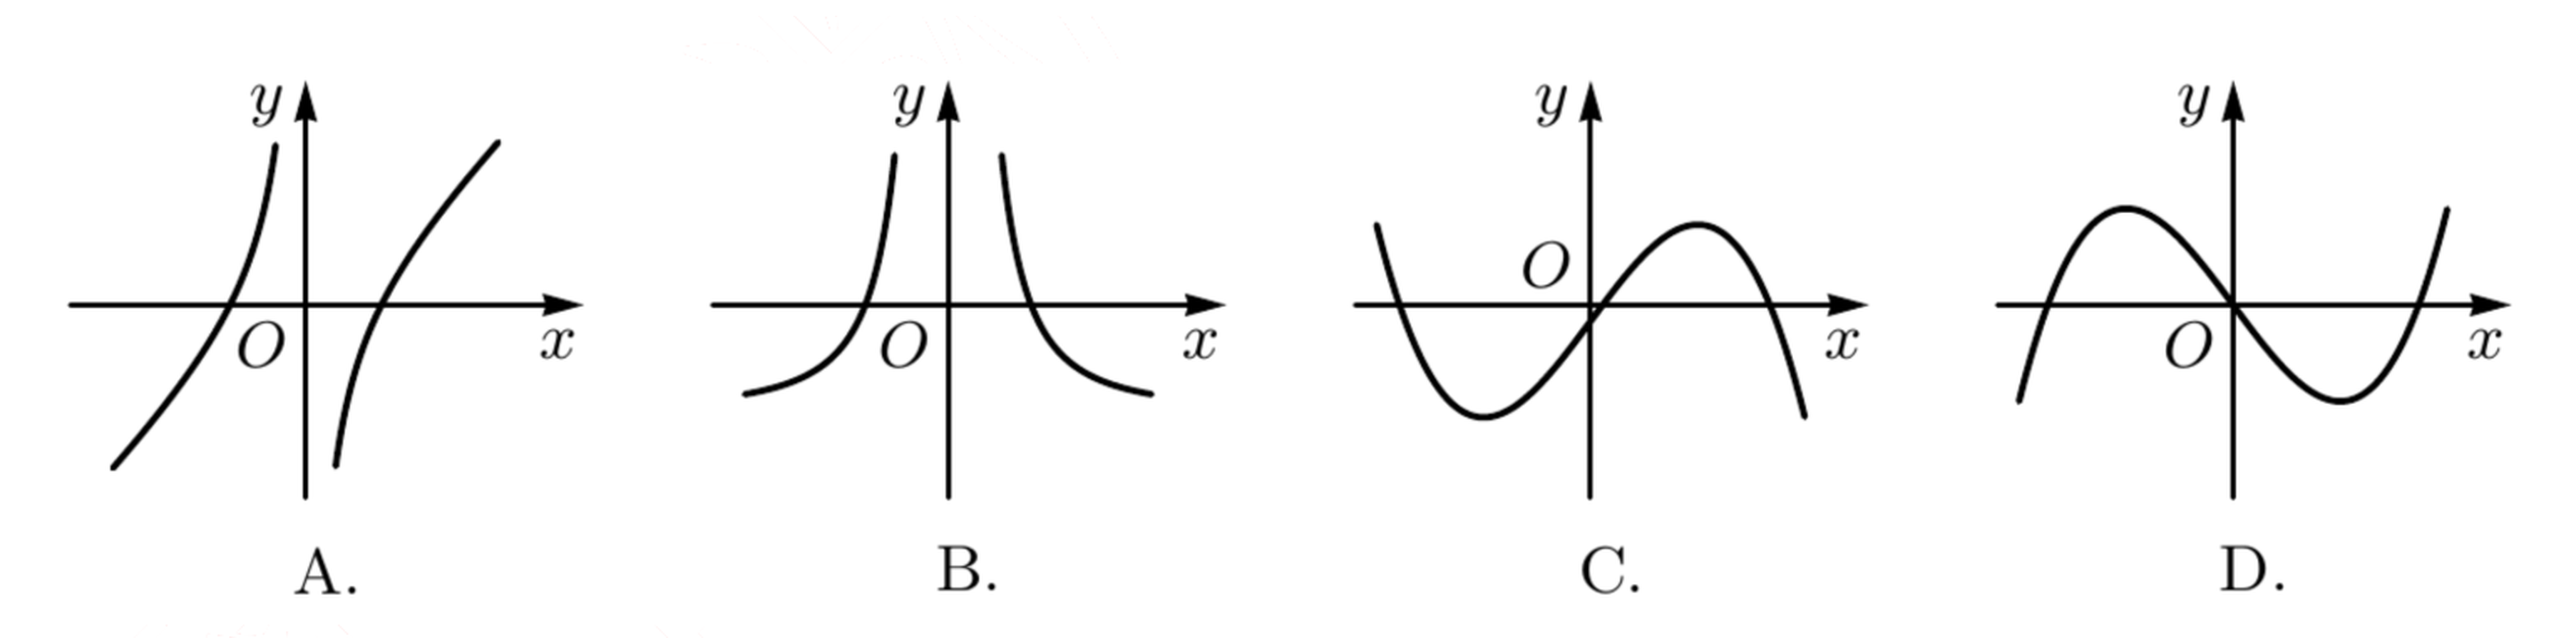
\includegraphics[width=0.90\textwidth]{figures/gao134_q13_options.png}
\end{center}

\ifanswer
\solbegin
\step{$f(x)$ 为偶函数，$g(x)$ 为奇函数，因此 $f(x)g(x)$ 为奇函数，排除 B.}
\step{又 $x=0$ 不在乘积函数的定义域内，其图象在 $y$ 轴上没有点，排除 C、D，}
\step{故选 $A$.}
\solend
\fi

\item 设全集为自然数集 $\N$，$E=\{x\mid x=2n,n\in\N\}$，$F=\{x\mid x=4n,n\in\N\}$，那么集合 $\N$ 可以表示成\mbox{（\quad）}

\keepwithprev
A. $E\cap F$\qquad\qquad B. $\overline{E}\cup F$\qquad\qquad C. $\overline{F}\cup E$\qquad\qquad D. $\overline{E}\cap\overline{F}$

\ifanswer
\solbegin
\step{$F\subseteq E$，所以 $\overline{F}\cup E=\N$，故选 $C$.}
\solend
\fi

\item 已知函数 $y=f(x)$，其中 $f(x)=x^2+bx$，则“$b<0$”是“$f(f(x))$ 的最小值与 $f(x)$ 的最小值相等”的\mbox{（\quad）}

\keepwithprev
A. 充分非必要条件\qquad\qquad B. 必要非充分条件

C. 充分必要条件\qquad\qquad D. 既非充分又非必要条件

\ifanswer
\solbegin
\step{$f(x)=\left(x+\dfrac b2\right)^2-\dfrac{b^2}4$，最小值为 $-\dfrac{b^2}4$，值域为 $\left[-\dfrac{b^2}4,+\infty\right)$.}
\step{当 $b<0$ 时，$-\dfrac b2>0\geqslant-\dfrac{b^2}4$，存在 $x$ 使 $f(x)=-\dfrac b2$，}
\step{从而 $f(f(x))$ 的最小值也为 $-\dfrac{b^2}4$，充分性成立.}
\step{当 $b=0$ 时，$f(x)=x^2$，$f(f(x))=x^4$，两者最小值均为 $0$，必要性不成立.}
\step{故选 $A$.}
\solend
\fi

\item 已知 $a,b,c\in\R$，若存在常数 $M>0$，使得 $a^2+b^2+c^2<M$，则称 $(a,b,c)$ 是有界数组. 对以下两个命题：

①若 $\lvert a^2+b+c\rvert+\lvert a^2+b-c\rvert\leqslant1$，则 $(a,b,c)$ 是有界数组；

②若 $\lvert a^2+b+c\rvert+\lvert a+b^2-c\rvert\leqslant1$，则 $(a,b,c)$ 是有界数组.% ②第二项为 \lvert a+b^2-c\rvert，与①刻意不同，照录

下列判断正确的是\mbox{（\quad）}

\keepwithprev
A. ①和②均为真命题\qquad\qquad B. ①和②均为假命题

C. ①为真命题，②为假命题\qquad D. ①为假命题，②为真命题

\ifanswer
\solbegin
\step{①取 $a=t,b=-t^2,c=0$，条件左端为 $0$，而 $a^2+b^2+c^2=t^2+t^4$ 可任意大，}
\step{故①为假命题.}
\step{②由条件，$a^2+a+b^2+b\leqslant\lvert a^2+b+c\rvert+\lvert a+b^2-c\rvert\leqslant1$.}
\step{由 $(a+1)^2+(b+1)^2\geqslant0$，得 $a^2+b^2\leqslant2(a^2+a+b^2+b)+2\leqslant4$.}
\step{又 $\lvert c\rvert\leqslant\lvert a^2+b+c\rvert+a^2+\lvert b\rvert\leqslant1+4+2=7$，故 $a^2+b^2+c^2\leqslant53<54$，}
\step{可取 $M=54$，故②为真命题.}
\step{故选 $D$.}
\solend
\fi

\end{enumerate}

\bigsec{三、解答题}

\begin{enumerate}
\setcounter{enumi}{16}

\item 已知不等式 $x^2-ax-b<0$ 的解集为 $A$，不等式 $\dfrac{3-2x}{x-1}<0$ 的解集为 $B$.

(1) 若 $a=5$，$b=-6$，求 $A\cap\overline{B}$；

(2) 若 $b=2a^2$，且 $A\cup B=B$，求实数 $a$ 的取值范围.

\ifanswer
\solbegin
\step{(1) 不等式 $\dfrac{3-2x}{x-1}<0$ 等价于 $x<1$ 或 $x>\dfrac32$，}
\step{所以 $B=(-\infty,1)\cup\left(\dfrac32,+\infty\right)$，$\overline{B}=\left[1,\dfrac32\right]$，}
\step{由 $x^2-5x+6=(x-2)(x-3)<0$，得 $A=(2,3)$，因此 $A\cap\overline{B}=\varnothing$.}
\step{(2) $A\cup B=B\Leftrightarrow A\subseteq B$，且 $x^2-ax-2a^2=(x-2a)(x+a)$，}
\step{当 $a=0$ 时，$A=\varnothing$，满足条件.}
\step{当 $a>0$ 时，$A=(-a,2a)$，$-a<0<1$，$A\subseteq B\Leftrightarrow2a\leqslant1$，得 $0<a\leqslant\dfrac12$.}
\step{当 $a<0$ 时，$A=(2a,-a)$，$2a<0<1$，$A\subseteq B\Leftrightarrow-a\leqslant1$，}
\step{得 $-1\leqslant a<0$.}
\step{因此 $a$ 的取值范围为 $\left[-1,\dfrac12\right]$.}
\solend
\fi

\item 为了在夏季降温和冬季供暖时减少能源损耗，房屋的屋顶和外墙需要建造隔热层. 某幢建筑物要建造可使用 $30$ 年的隔热层，每厘米厚的隔热层建造成本为 $9$ 万元. 该建筑物每年的能源消耗费用 $C$（万元）与隔热层厚度 $x$（cm）满足如下关系式：$C=\dfrac{k}{3x+5}$（$0\leqslant x\leqslant10$）. 若不建隔热层，每年能源消耗费用为 $8$ 万元. 设 $y$（万元）为隔热层建造费用与 $30$ 年的能源消耗费用之和.

(1) 求 $k$ 的值及 $y$ 的表达式；

(2) 隔热层修建多厚时，总费用 $y$ 最小？并求最小值.

\ifanswer
\solbegin
\step{(1) 不建隔热层时 $x=0$，$C=8$，所以 $\dfrac k5=8$，得 $k=40$.}
\step{隔热层建造费用为 $9x$ 万元，$30$ 年的能源消耗费用为 $30\times\dfrac{40}{3x+5}$ 万元.}
\step{因此 $y=9x+\dfrac{1200}{3x+5}$，$0\leqslant x\leqslant10$.}
\step{(2) 令 $t=3x+5$，则 $5\leqslant t\leqslant35$，且 $y=3t+\dfrac{1200}{t}-15$，}
\step{因为 $t>0$，由基本不等式得 $y\geqslant2\sqrt{3t\cdot\dfrac{1200}{t}}-15=105$，}
\step{当且仅当 $3t=\dfrac{1200}{t}$，即 $t=20$时取等号，此时 $x=5\in[0,10]$，}% 原卷"20"与"时"之间未留空，照录
\step{所以隔热层厚度为 $5$ cm 时，总费用最小，最小值为 $105$ 万元.}
\solend
\fi

\item 已知 $f(x)=ax^2+\dfrac1x$，其中 $a$ 为常数.

(1) 若 $a\in(1,3)$，判断函数 $y=f(x)$ 在 $[1,2]$ 上的单调性，并用定义证明；

(2) 求函数 $y=f(x)-x-\dfrac1x$ 在 $[1,2]$ 上的最大值 $g(a)$.

\ifanswer
\solbegin
\step{(1) 任取 $x_1,x_2\in[1,2]$，且 $x_1<x_2$，}
\step{则 $f(x_2)-f(x_1)=(x_2-x_1)\left[a(x_1+x_2)-\dfrac1{x_1x_2}\right]$，}
\step{由 $a>1$，$x_1+x_2\geqslant2$，$x_1x_2\geqslant1$，得 $a(x_1+x_2)-\dfrac1{x_1x_2}>2-1>0$，}
\step{因此 $f(x_2)>f(x_1)$，$f(x)$ 在 $[1,2]$ 上为严格增函数.}
\step{(2) 令 $h(x)=f(x)-x-\dfrac1x=ax^2-x$，其中 $x\in[1,2]$.}
\step{若 $a=0$，则 $h(x)=-x$，所以 $h(x)_{max}=h(1)=-1$；}
\step{若 $a<0$，二次函数的图象的对称轴为 $x=\dfrac1{2a}<0$，}
\step{所以 $y=h(x)$ 在 $[1,2]$ 上是严格减函数，所以 $h(x)_{max}=h(1)=a-1$；}
\step{若 $a>0$ 且 $\dfrac1{2a}>\dfrac32$，即 $0<a<\dfrac13$ 时，$h(x)_{max}=h(1)=a-1$.}
\step{若 $a>0$ 且 $\dfrac1{2a}\leqslant\dfrac32$，即 $a\geqslant\dfrac13$ 时，$h(x)_{max}=h(2)=4a-2$.}
\step{综上所述，$g(a)=\begin{cases}a-1,a<\dfrac13\\4a-2,a\geqslant\dfrac13\end{cases}$.}
\solend
\fi

\item 已知 $f(x)=\dfrac{ax^2+1}{bx+c}$（$a,b,c\in\Z$）.

(1) 若函数 $y=f(x)$ 是奇函数，且 $f(1)=2$，$f(2)<3$，求 $a,b,c$ 的值；

(2) 若函数 $y=f(x)$ 是偶函数，且 $ac<0$，$f(2a^2+a+1)<f(-3a^2+2a-1)$，求 $a$ 的值；

(3) 若 $b=a+c^2$，且满足不等式 $\lvert f(x)\rvert\geqslant1$ 的 $x$ 的最大值为 $0$，求 $c$ 的值.

\ifanswer
\solbegin
\step{(1) 由 $f(-x)=-f(x)$，交叉相乘得 $2c(ax^2+1)=0$ 恒成立，}
\step{因此 $c=0$，$b\neq0$.}
\step{由 $f(1)=2$，得 $a+1=2b$，}
\step{于是 $f(2)=\dfrac{4a+1}{2b}=4-\dfrac3{2b}<3\Leftrightarrow0<b<\dfrac32$，}
\step{因为 $b\in\Z$，所以 $b=1$，进而 $a=1$，$c=0$.}
\step{(2) 由 $f(-x)=f(x)$，交叉相乘得 $2bx(ax^2+1)=0$ 恒成立，因此 $b=0$.}
\step{此时 $f(x)=\dfrac ac x^2+\dfrac1c$，且 $\dfrac ac<0$.}
\step{设 $u=2a^2+a+1$，$v=-3a^2+2a-1$.}
\step{方程 $2a^2+a+1=0$ 与 $3a^2-2a+1=0$ 的判别式分别为 $-7$ 与 $-8$，}
\step{都小于 $0$，所以 $u>0$，$v<0$.}
\step{于是 $f(u)<f(v)\Leftrightarrow u^2>v^2\Leftrightarrow u>-v\Leftrightarrow-a^2+3a>0\Leftrightarrow0<a<3$，}
\step{因为 $a\in\Z$，所以 $a=1$ 或 $a=2$.}
\step{(3) 因为解集的最大值为 $0$，所以 $f(0)$ 有定义且 $\lvert f(0)\rvert\geqslant1$，}
\step{即 $c\neq0$，$\left\lvert\dfrac1c\right\rvert\geqslant1$，结合 $c\in\Z$，得 $c=\pm1$，从而 $b=a+1$.}
\step{当 $x=2$ 时，分母 $2a+2+c$ 为奇数，必不为 $0$；}
\step{又因为 $2>0$，必须有 $\lvert f(2)\rvert<1\Leftrightarrow\lvert4a+1\rvert<\lvert2a+2+c\rvert$，}
\step{若 $c=-1$，则 $(4a+1)^2<(2a+1)^2\Leftrightarrow4a(3a+1)<0\Leftrightarrow-\dfrac13<a<0$，}
\step{不存在满足条件的整数 $a$.}
\step{若 $c=1$，则 $(4a+1)^2<(2a+3)^2\Leftrightarrow4(3a+2)(a-1)<0\Leftrightarrow-\dfrac23<a<1$，}
\step{所以 $a=0$，$b=1$，此时 $f(x)=\dfrac1{x+1}$，}
\step{且 $\lvert f(x)\rvert\geqslant1\Leftrightarrow0<\lvert x+1\rvert\leqslant1\Leftrightarrow x\in[-2,-1)\cup(-1,0]$，}
\step{解集的最大值确为 $0$，因此 $c=1$.}
\solend
\fi

\item 已知函数 $y=f(x)$ 的定义域为 $\R$，且当 $x>0$ 时，$f(x)=\dfrac1{x+1}$. 对任意 $x_0\in\R$，定义集合 $D(x_0)=\{d\mid f(x_0+d)>f(x_0)\}$.

(1) 若当 $x\leqslant0$ 时，$f(x)=-2x+1$，求函数 $y=f(x)$ 的值域；

(2) 若 $y=f(x)$ 是偶函数，且 $f(0)=1$，求证：$D(-2)=\{-d\mid d\in D(2)\}$；

(3) 若 $y=f(x)$ 是奇函数，且 $x_1x_2\neq0$，求证：“$f(x_1)\leqslant f(x_2)$”的充要条件是\!\mbox{“$D(x_2)\subseteq D(x_1)$”}.

\ifanswer
\solbegin
\step{(1) 当 $x>0$ 时，$0<f(x)<1$；当 $x\leqslant0$ 时，$f(x)=-2x+1\geqslant1$.}
\step{函数的值域为 $(0,1)\cup[1,+\infty)=(0,+\infty)$.}
\step{(2) 由 $f(x)$ 是偶函数及 $f(0)=1$，得 $f(x)=\dfrac1{1+\lvert x\rvert}$，且 $f(2)=f(-2)=\dfrac13$.}
\stepm{法一：}{$D(2)=\left\{d\mid\dfrac1{1+\lvert2+d\rvert}>\dfrac13\right\}=\{d\mid\lvert2+d\rvert<2\}=(-4,0)$，}
\step{$D(-2)=\left\{d\mid\dfrac1{1+\lvert-2+d\rvert}>\dfrac13\right\}=\{d\mid\lvert-2+d\rvert<2\}=(0,4)$，}
\step{因此 $\{-d\mid d\in D(2)\}=(0,4)=D(-2)$.}
\stepm{法二：}{任取 $d\in D(-2)$，由定义得 $f(-2+d)>f(-2)$.}
\step{因为 $y=f(x)$ 是偶函数，所以对任意的实数 $x$，有 $f(-x)=f(x)$，}
\step{因此 $f(-2+d)=f(-(-2+d))=f(2-d)$，且 $f(-2)=f(2)$.}
\step{所以不等式 $f(-2+d)>f(-2)$ 等价于 $f(2-d)>f(2)$，}
\step{这恰好是 $-d\in D(2)$ 的定义，}
\step{所以 $d\in D(-2)\Leftrightarrow-d\in D(2)$，故 $D(-2)=\{-d\mid d\in D(2)\}$.}
\step{(3) 由 $f(x)$ 是奇函数，得 $f(0)=0$；}
\step{当 $x<0$ 时，$f(x)=-f(-x)=-\dfrac1{1-x}=\dfrac1{x-1}$；}
\step{所以 $f(x)=\begin{cases}\dfrac1{x-1},&x<0\\0,&x=0;\\\dfrac1{x+1},&x>0\end{cases}$}
% 2026-11-15 回原图订正：原卷 11 页此 cases 块末无句点，本稿初转顺手补了西文句点，今删去（Q19 08 页同类块末有句点，照录保留）。
\step{当 $x_0<0$ 时，$D(x_0)=\{d\mid f(x_0+d)>f(x_0)\}=(-\infty,0)\cup[-x_0,+\infty)$，}
\step{当 $x_0=0$ 时，$D(0)=\{d\mid f(0+d)>f(0)\}=(0,+\infty)$，}
\step{当 $x_0>0$ 时，$D(x_0)=\{d\mid f(x_0+d)>f(x_0)\}=(-x_0,0)$.}
\stepm{先证明必要性.}{若 $f(x_1)\leqslant f(x_2)$，仅需讨论三类情形：}
\step{若 $x_2\leqslant x_1<0$，}
\step{则 $D(x_1)=(-\infty,0)\cup[-x_1,+\infty),D(x_2)=(-\infty,0)\cup[-x_2,+\infty)$，}
\step{故 $D(x_2)\subseteq D(x_1)$；}
\step{若 $0<x_2\leqslant x_1$，则 $D(x_1)=(-x_1,0),D(x_2)=(-x_2,0)$，}
\step{故 $D(x_2)\subseteq D(x_1)$；}
\step{若 $x_1<0<x_2$，则 $D(x_1)=(-\infty,0)\cup[-x_1,+\infty),D(x_2)=(-x_2,0)$，}
\step{故 $D(x_2)\subseteq D(x_1)$.}
\stepm{再证明充分性.}{若 $D(x_2)\subseteq D(x_1)$，}
\step{若 $x_1<0,x_2<0$，}
\step{则 $D(x_1)=(-\infty,0)\cup[-x_1,+\infty),D(x_2)=(-\infty,0)\cup[-x_2,+\infty)$，}
\step{由 $D(x_2)\subseteq D(x_1)$ 得 $x_2\leqslant x_1$，}
\step{又 $y=f(x)$ 在 $(-\infty,0)$ 上是严格减函数，所以 $f(x_1)\leqslant f(x_2)$；}
\step{若 $x_1>0,x_2>0$，则 $D(x_1)=(-x_1,0),D(x_2)=(-x_2,0)$，}
\step{由 $D(x_2)\subseteq D(x_1)$ 得 $x_2\leqslant x_1$，}
\step{又 $y=f(x)$ 在 $(0,+\infty)$ 上是严格减函数，所以 $f(x_1)\leqslant f(x_2)$；}
\step{若 $x_1<0,x_2>0$，则 $f(x_1)<0<f(x_2)$，结论成立；}
\step{若 $x_1>0,x_2<0$，此时 $D(x_1)=(-x_1,0)$ 中只有负数，}
\step{而 $D(x_2)=(-\infty,0)\cup[-x_2,+\infty)$ 中有正数，$D(x_2)\subseteq D(x_1)$ 不成立.}
\step{综上，“$f(x_1)\leqslant f(x_2)$”的充要条件是“$D(x_2)\subseteq D(x_1)$”.}
\solend
\fi

\end{enumerate}

\end{document}
"
% 紧凑版：xelatex "\def\iscompact{1}% 高一134_华师大二附中_期中.tex
%   —— 高一上数学"2026-2027 年华师大二附中高一上期中"（试卷版/答案版）
% 试卷版：xelatex 高一134_华师大二附中_期中.tex
% 答案版：xelatex "\def\isanswer{1}% 高一134_华师大二附中_期中.tex
%   —— 高一上数学"2026-2027 年华师大二附中高一上期中"（试卷版/答案版）
% 试卷版：xelatex 高一134_华师大二附中_期中.tex
% 答案版：xelatex "\def\isanswer{1}\input{高一134_华师大二附中_期中.tex}"
% 紧凑版：xelatex "\def\iscompact{1}\input{高一134_华师大二附中_期中.tex}"
%
% ① 原始材料：微信公众号"魔都数学加油站"文章，作者破晓，2026-11-15 18:04 发布；
% 连载"27学年高一134"，原文标题"27学年高一134——2026-2027年上海市华师大二附中高一上期中"；
% 原文链接：https://mp.weixin.qq.com/s/bQlkmlGdCtAlytY331vf3g。
% 正文为 13 张 PNG 页（01、04、06、08、09、10、11、12、13 为 2560x3620；
% 02、03、05、07 为 4762x6735，同一篇各页分辨率不同，逐页按各自分辨率裁图核对），
% 题目下印有【解析】，为讲评版。题目、解析均据原图转录；卷面粉红色水印
% "魔都数学加油站"及公众号页脚未录入。
% 全卷 2 幅插图，均在第 04 页：第 13 题题干 y=f(x)、y=g(x) 两幅函数图象合并裁为
% figures/gao134_q13_graphs.png，第 13 题 A/B/C/D 四幅函数图象选项合并裁为
% figures/gao134_q13_options.png；两图均取原卷 04 页截图 3× LANCZOS 放大、
% 白化粉色水印（只白化浅粉色 R>175 且 G>140 且 B>140 的像素，保留红色标签）。
% 注意：本卷 Q13 四幅选项在原卷排为"一行四幅"（1×4），并非 高一132 第 14 题
% 的 2×2 排布，本稿按原卷 1×4 合并裁为一张，不重排、不用 TikZ 重绘。
%
% 卷首标题：原卷印作"2026-2027 年华师大二附中高一上期中"（公众号标题中的"上海市"
% 卷面标题行没有，本稿照卷面），年份区间按全稿惯例排 en dash；原卷未印副标题，
% 本卷为期中卷、跨集合与常用逻辑用语／不等式／函数三章，按题目内容标为
% "集合与常用逻辑用语、不等式、函数"（与 125／126／128／129／131／132／133 同期中卷口径相同）：
% 集合与逻辑见 Q6、Q10、Q14、Q16、Q17、Q21，不等式见 Q3、Q7、Q9、Q11、Q15、Q18、Q19，
% 函数（函数性质、二分法、奇偶性、基本不等式应用）见 Q4、Q5、Q8、Q12、Q13、Q20。
%
% 题号体例：本卷共 19 题——一、填空题 3—12（10 题）、二、选择题 13—16（4 题）、
% 三、解答题 17—21（5 题）。三节分别 \setcounter{enumi}{2}／{12}／{16}。
% 第 13 页仅为 Q21 (3) 解析续尾，全卷无「四、附加题」。
%
% ② 与原卷的排版差异：
%   ① 原文从第 3 题起，本稿保留原题号（见上"题号体例"）；
%   ② 原卷每题下直接印【解析】，本稿按全稿惯例置于答案版；第 13—16 题答案均在
%      解析末句"故选 …"，题干括号内留空、不另提 \ans{}（四题均无独立答案段）；
%      全卷无只印括号内答案、无解析的选择题；
%   ③ 原卷未印副标题，本稿按"知识模块"口径补出；
%   ④ 原卷填空横线按全稿惯例排为 \blankline[4.4em]；选择题括号排 \mbox{（\quad）}、
%      每个选项段前按惯例加 \keepwithprev（Q13 四选项为图，守卫前行为 \begin{center}；
%      Q15、Q16 四选项分两行排，\keepwithprev 只加在 A. 行前）；解答题不留作答区、
%      不加 \anspace（原卷为讲评版，与 129／131／132／133 同）；
%   ⑤ 原卷数集印黑板粗体（Q7／Q11／Q12／Q16／Q21 的 R、Q14／Q20 的 N、Q20 的 Z），
%      按全稿惯例统一排 \R／\N／\Z；绝对值排 \lvert…\rvert，集合描述竖线排 \mid；不等号按全稿惯例排
%      \leqslant／\geqslant；补集照原卷上划线排 \overline{B}、\overline{E}、\overline{F}；
%   ⑥ 子题标号 (1)(2)(3) 与括注原卷均用半角括号，照录（与 131／132／133 同）；
%      圈数字 ①② 照录；原卷 Q21 (2) 解析"法一：""法二："与 Q21 (3) 解析
%      "先证明必要性.""再证明充分性."四处标签印红色加粗，按 高一53／108／133 成例排
%      \stepm{法一：}／\stepm{法二：}／\stepm{先证明必要性.}／\stepm{再证明充分性.}
%      （加粗着色、不引入红色，不动 common.sty）；Q8 解析"第 1 步：""第 2 步：""
%      "第 3 步："原卷印黑色常规宋体（非红非粗），照录为普通 \step 行内文字；
%   ⑦ 数学式内半角逗号照录（如 Q6 $A=\{0,1,2,3\}$、Q14 $x=2n,n\in\N$、
%      Q16 $a,b,c\in\R$ 与 $a=t,b=-t^2,c=0$、Q19 $x_1,x_2\in[1,2]$、
%      Q20 $a,b,c\in\Z$、Q21 $x_1<0,x_2<0$ 与 $D(x_1)=(-x_1,0),D(x_2)=(-x_2,0)$）；
%      原卷行末全角句点按全稿惯例从宽排西文句点；cases 块末的句点逐处照录：
%      Q19 解析（08 页）块末原卷有句点照录、Q21 (3) 解析（11 页）块末原卷无句点不补，
%      两处原卷自身不统一（2026-11-15 回原图核对，本稿初转曾顺手补句点，已删去）；
%   ⑧ 原卷 Q8 解析跨 01—02 页、Q10 解析跨 02—03 页、Q12 解析跨 03—04 页、
%      Q16 解析跨 05—06 页、Q17 解析跨 06—07 页、Q20 解析跨 08—10 页、
%      Q21 解析跨 10—13 页，本稿按题合并连续排版；末页第 13 页为
%      Q21 (3) 解析续尾与"综上"一句，按实际印刷行单列；
%   ⑨ 题干中的中文弯引号按原卷照录（Q10 研究问题、Q15 条件、Q21 (3) 充要条件），
%      注释内一律 ASCII 引号。
%
% 判别式字形：全卷仅 Q9 解析末行出现一处判别式记号
%   "两值均满足 $\Delta=p^2-4p=18\mp12\sqrt2>0$"，逐处放大核对，原卷印高三角
%   $\Delta$（等腰、高，实测高宽比约 1.14），照录 \Delta；卷内无扁三角 \triangle，
%   与 高一132 同题排 $\triangle$、高一133 部分判别式排 $\triangle$ 均不同。
%
% 子集符号：Q6 题干 $C\subseteq A$、$C\subseteq B$ 与解析 $C\subseteq A\cap B$、
%   Q14 解析 $F\subseteq E$、Q17 解析 $A\subseteq B$、Q21 题干与解析各处的
%   $D(x_2)\subseteq D(x_1)$，全部印带下划线的 $\subseteq$，逐处放大核对，
%   照录 \subseteq；全卷未出现单线 \subset。
%
% 原卷存疑照录（均照录未改，正文对应处另有 % 注）：
%   第 6 题题干集合 $A=\{0,1,2,3\}$ 三个逗号后不留空，紧邻的 $B=\{0,2,4,5\}$
%      三个逗号后却留空，同卷同一行两集合排字不一，照录其逗号均为半角；
%   第 16 题命题②作 $\lvert a^2+b+c\rvert+\lvert a+b^2-c\rvert\leqslant1$，
%      与命题①第二项 $\lvert a^2+b-c\rvert$ 不同（①无 $b$ 的平方、②有），
%      两命题刻意不同，照录；解析"②由条件，$a^2+a+b^2+b\leqslant\cdots$"
%      由两项相加直接得到，照录；
%   第 18 题 (2) 解析"即 $t=20$时取等号"中"20"与"时"之间原卷未留空，照录；
%   第 19 题解析 $h(x)_{max}$ 的"max"下标三处字形不一（斜体／正体混排），照录；
%   第 20 题 (1)(2) 解析"由 $f(-x)=-f(x)$，交叉相乘得……"与"由 $f(-x)=f(x)$，
%      交叉相乘得……"两处措辞照录；
%   第 21 题 (2) 原卷并存"法一"（集合计算）与"法二"（定义推证）两套证明，照录不删。
%
% 行数复核：逐题数 \step/\stepm 条数，合计 134 条（Q3：2；Q4：1；Q5：1；Q6：1；
% Q7：2；Q8：4；Q9：3；Q10：4；Q11：5；Q12：8；Q13：3；Q14：1；Q15：5；
% Q16：7；Q17：9；Q18：7；Q19：11；Q20：22；Q21：38），与原卷印刷行逐题相等
% （cases 块作一个印刷行计）。第 13—16 题答案在解析末句，括号内留空、不另提 \ans{}；
% 第 21 题四条 \stepm 计入 38 条内。
%
\documentclass[a4paper,11pt]{article}
\usepackage{common}

\begin{document}

\examtitlest[3]{2026--2027 年华师大二附中高一上期中}{集合与常用逻辑用语、不等式、函数}

\bigsec{一、填空题}

\begin{enumerate}
\setcounter{enumi}{2}

\item 不等式 $\lvert 2x+1\rvert\geqslant3$ 的解集为\blankline[4.4em].

\ifanswer
\solbegin
\step{$\lvert 2x+1\rvert\geqslant3\Leftrightarrow 2x+1\leqslant-3$ 或 $2x+1\geqslant3\Leftrightarrow x\leqslant-2$ 或 $x\geqslant1$，}
\step{故解集为 $(-\infty,-2]\cup[1,+\infty)$.}
\solend
\fi

\item 函数 $y=\sqrt{x+1}+\dfrac1x$ 的定义域为\blankline[4.4em].

\ifanswer
\solbegin
\step{$x+1\geqslant0$ 且 $x\neq0$，得定义域为 $[-1,0)\cup(0,+\infty)$.}
\solend
\fi

\item 已知等式 $3x^2-4x-2=a(x-1)^2+b(x-1)+c$ 恒成立，其中 $a$、$b$、$c$ 为常数，则 $a-b+c=$\blankline[4.4em].

\ifanswer
\solbegin
\step{令 $x=0$，得 $a-b+c=-2$.}
\solend
\fi

\item 已知集合 $A=\{0,1,2,3\}$，$B=\{0,2,4,5\}$，$C\subseteq A$，$C\subseteq B$，符合条件的集合 $C$ 有\blankline[4.4em]个.% 原卷 A 的逗号后不留空、B 的逗号后留空，排字不一，照录

\ifanswer
\solbegin
\step{$C\subseteq A\cap B=\{0,2\}$，所以符合条件的集合 $C$ 有 $2^2=4$ 个.}
\solend
\fi

\item 设 $a$、$b\in\R$，且 $a^2+4b^2=2$，则 $ab$ 的最大值为\blankline[4.4em].

\ifanswer
\solbegin
\step{$(a-2b)^2=a^2+4b^2-4ab=2-4ab\geqslant0$，得 $ab\leqslant\dfrac12$，}
\step{当且仅当 $a=2b=\pm1$ 时取等号，故 $ab$ 的最大值为 $\dfrac12$.}
\solend
\fi

\item 已知函数 $y=x(13-2x)^2-140$，用二分法求函数在区间 $(3,4)$ 上的零点时，第 3 步应计算 $x=$\blankline[4.4em]的函数值.

\ifanswer
\solbegin
\step{记 $f(x)=x(13-2x)^2-140$，则 $f(3)=7>0$，$f(4)=-40<0$.}
\step{第 1 步：$f\left(\dfrac72\right)=-14<0$，区间缩小为 $\left(3,\dfrac72\right)$.}
\step{第 2 步：$f\left(\dfrac{13}4\right)=-\dfrac{43}{16}<0$，区间缩小为 $\left(3,\dfrac{13}4\right)$.}
\step{第 3 步：应计算 $x=\dfrac{3+\frac{13}4}2=\dfrac{25}8$ 的函数值.}
\solend
\fi

\item 已知一元二次方程 $x^2+px+p=0$ 的两个实根分别为 $x_1$、$x_2$，且 $x_1^2x_2+x_2^2x_1=-18$，则 $p=$\blankline[4.4em].% 判别式 \Delta 高三角，逐处放大核对

\ifanswer
\solbegin
\step{由韦达定理，$x_1+x_2=-p$，$x_1x_2=p$，}
\step{则 $x_1^2x_2+x_2^2x_1=x_1x_2(x_1+x_2)=-p^2=-18\Rightarrow p=\pm3\sqrt2$，}
\step{两值均满足 $\Delta=p^2-4p=18\mp12\sqrt2>0$，故 $p=\pm3\sqrt2$.}
\solend
\fi

\item 研究问题：“已知关于 $x$ 的不等式 $ax^2-bx+c>0$ 的解集为 $(1,2)$，解关于 $x$ 的不等式 $cx^2-bx+a>0$”，有如下解法：

解：由 $ax^2-bx+c>0\Rightarrow a-b\left(\dfrac1x\right)+c\left(\dfrac1x\right)^2>0$，令 $y=\dfrac1x$，则 $y\in\left(\dfrac12,1\right)$，

所以不等式 $cx^2-bx+a>0$ 的解集为 $\left(\dfrac12,1\right)$.

参考上述解法，已知关于 $x$ 的不等式 $\dfrac{k}{x+a}+\dfrac{x+b}{x+c}<0$ 的解集为 $(-3,-1)\cup(2,4)$，则关于 $x$ 的不等式 $\dfrac{kx}{ax-1}+\dfrac{bx-1}{cx-1}<0$ 的解集为\blankline[4.4em].

\ifanswer
\solbegin
\step{当 $x=0$ 时，所求不等式左端为 $1$，不满足不等式.}
\step{当 $x\neq0$ 时，两个分式的分子、分母同除以 $x$，得 $\dfrac{k}{a-\frac1x}+\dfrac{b-\frac1x}{c-\frac1x}<0$.}
\step{令 $t=-\dfrac1x$，则所求不等式化为 $\dfrac{k}{t+a}+\dfrac{t+b}{t+c}<0$，即 $-\dfrac1x\in(-3,-1)\cup(2,4)$，}
\step{解得 $x\in\left(-\dfrac12,-\dfrac14\right)\cup\left(\dfrac13,1\right)$.}
\solend
\fi

\item 已知 $a\in(0,+\infty)$，若对任意的 $x\in(0,+\infty)$，均有 $\lvert x^2-a\rvert+\lvert x+b\rvert=\lvert x^2+x-a+b\rvert$，则 $a^2-b^2$ 的最小值为\blankline[4.4em].

\ifanswer
\solbegin
\step{原等式成立的充要条件是 $(x^2-a)(x+b)\geqslant0$.}
\step{当 $0<x<\sqrt a$ 时须有 $x+b\leqslant0$；当 $x>\sqrt a$ 时须有 $x+b\geqslant0$，因此 $b=-\sqrt a$.}
\step{此时 $(x^2-a)(x+b)=(x+\sqrt a)(x-\sqrt a)^2\geqslant0$，满足题意.}
\step{$a^2-b^2=a^2-a=\left(a-\dfrac12\right)^2-\dfrac14\geqslant-\dfrac14$，}
\step{当 $a=\dfrac12$，$b=-\dfrac{\sqrt2}2$ 时取等号，最小值为 $-\dfrac14$.}
\solend
\fi

\item 已知函数 $y=f(x)$ 在 $\R$ 上是严格增函数，当 $x\neq0$ 且 $f(x)\neq0$ 时，满足 $f(x)\cdot f\left[\dfrac1{f(x)}+\dfrac1x\right]=1$，则 $f(1)=$\blankline[4.4em].

\ifanswer
\solbegin
\step{当 $xf(x)>0$ 时，记 $t=\dfrac1{f(x)}+\dfrac1x\neq0$，则 $f(t)=\dfrac1{f(x)}\neq0$.}
\step{将 $t$ 代入题设，得 $f\left(f(x)+\dfrac1t\right)=f(x)$，严格增性给出 $f(x)+\dfrac1t=x$，}
\step{化简得 $f(x)^2+xf(x)-x^2=0$，由 $\dfrac{f(x)}x>0$ 得 $f(x)=\dfrac{\sqrt5-1}2x$.}
\step{设 $a=f(0)$，若 $a>0$，则 $f(a)>f(0)=a>0$；}
\step{若 $a<0$，则 $f(a)<f(0)=a<0$.}
\step{两种情形都有 $af(a)>0$ 且 $\dfrac{f(a)}a>1$，与上式 $\dfrac{f(a)}a=\dfrac{\sqrt5-1}2<1$ 矛盾，}
\step{因此 $f(0)=0$.}
\step{于是 $f(1)>0$，代入上式得 $f(1)=\dfrac{\sqrt5-1}2$.}
\solend
\fi

\end{enumerate}

% 第 13 题是"节标题 + 题干 + 两幅图 + 四幅选项图"约 15cm 的整块，
% 守卫只放在 \bigsec 之前；若再在 \item 之前放第二枚，会在标题已印出后才触发换页，
% 把题目推走、留下孤立节标题（切页审计 B 类）。高度须覆盖整块。
\needvspace{16cm}
\bigsec{二、选择题}

\begin{enumerate}
\setcounter{enumi}{12}

\item 已知函数 $y=f(x)$ 与 $y=g(x)$ 的图象如图所示，则函数 $y=f(x)\cdot g(x)$ 的图象可能是\mbox{（\quad）}

\keepwithprev
\begin{center}
% 题干 y=f(x)、y=g(x) 两幅函数图象取原卷 04 页截图去粉色水印，按原卷左右排布合并为一张
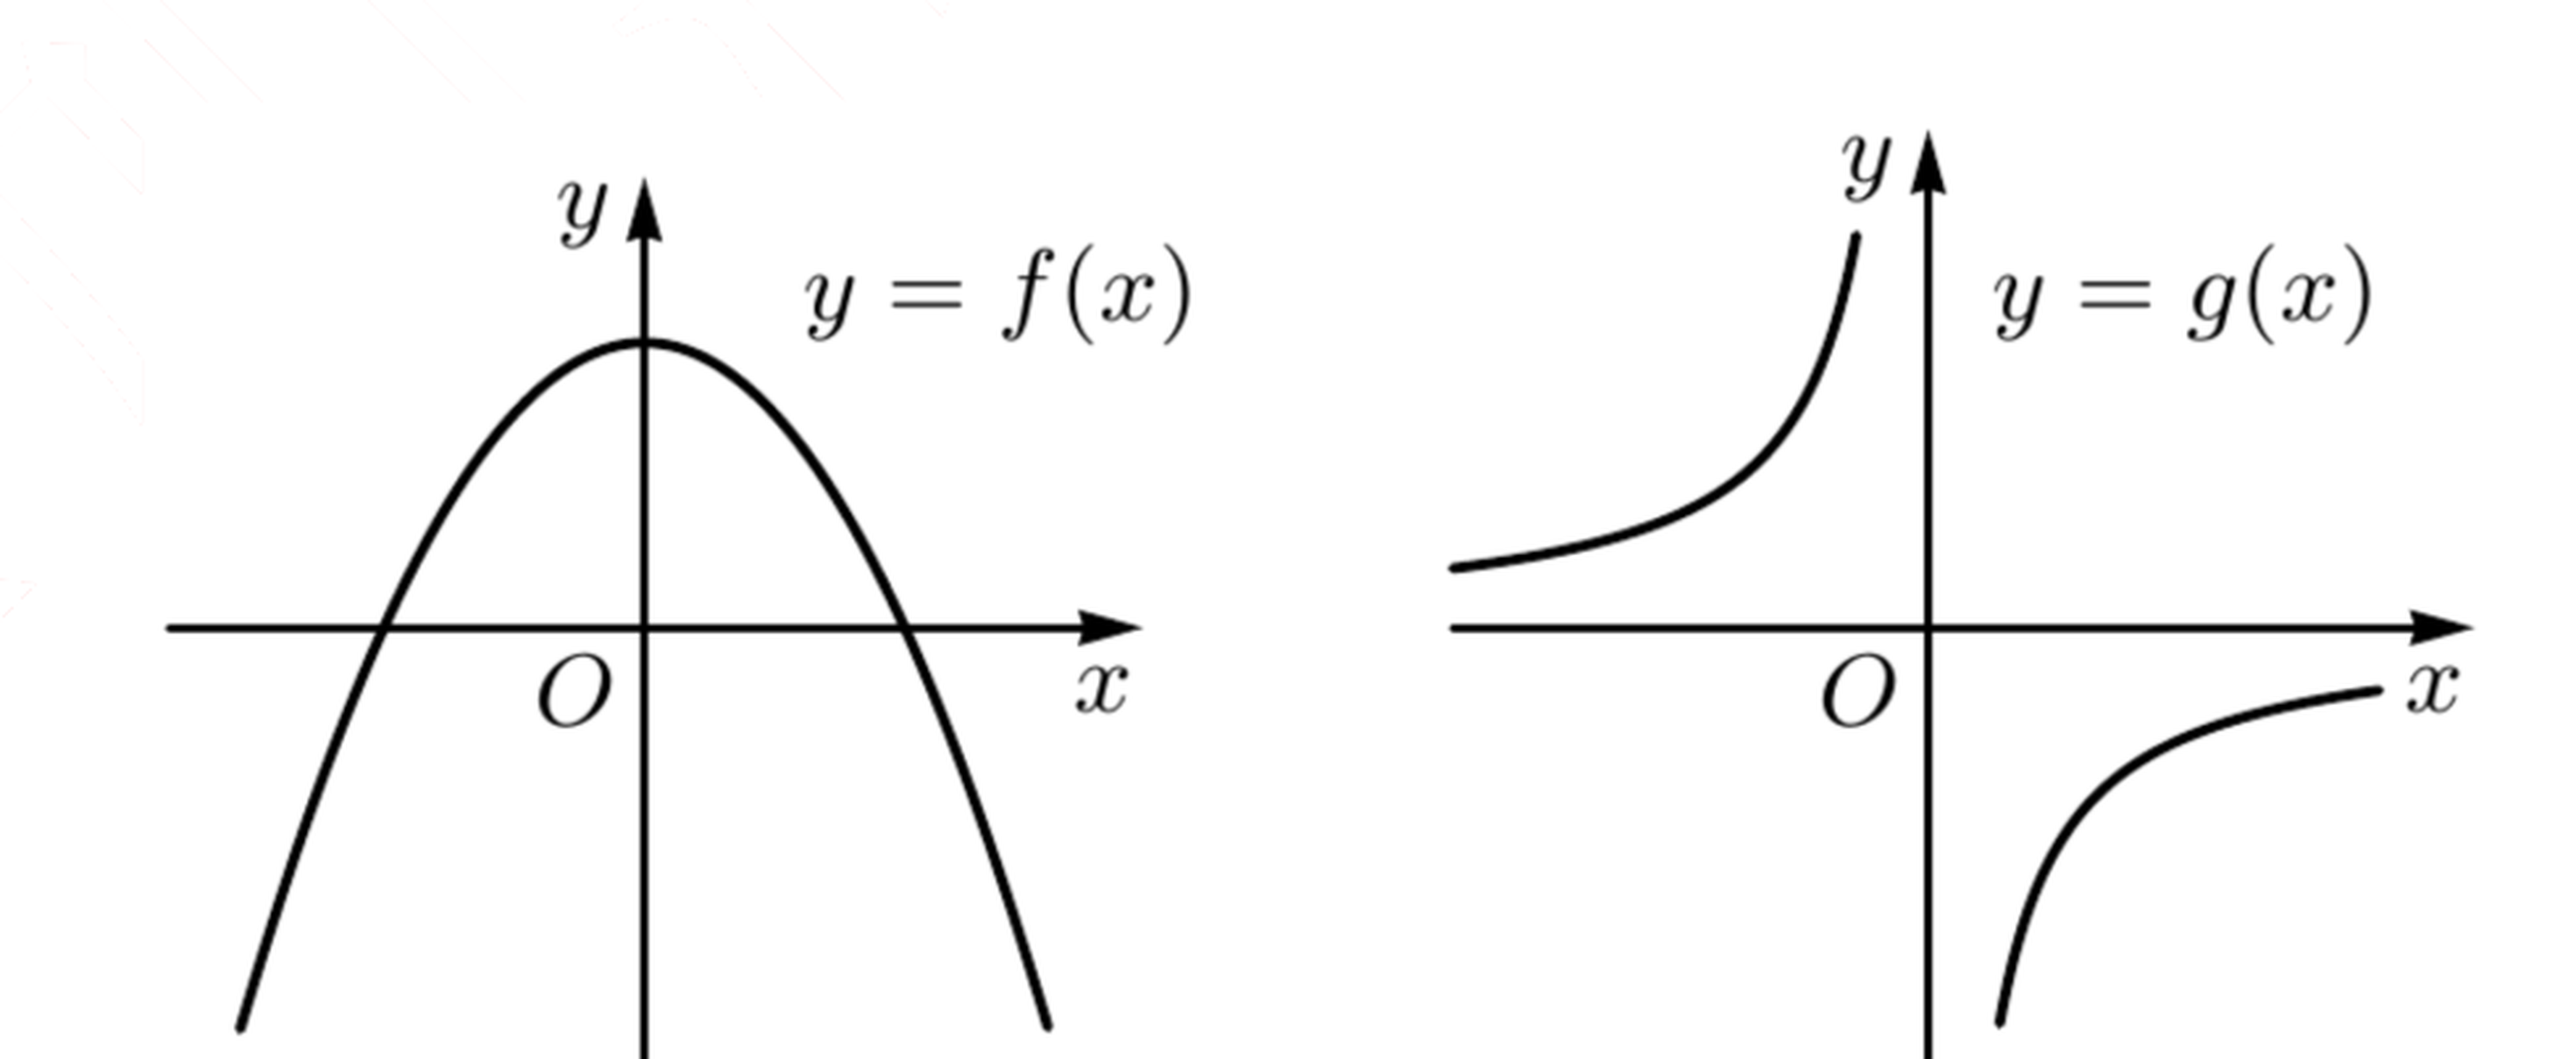
\includegraphics[width=0.72\textwidth]{figures/gao134_q13_graphs.png}\\[0.6em]
% A/B/C/D 四幅函数图象选项取原卷 04 页截图去粉色水印，按原卷一行四幅排布合并为一张
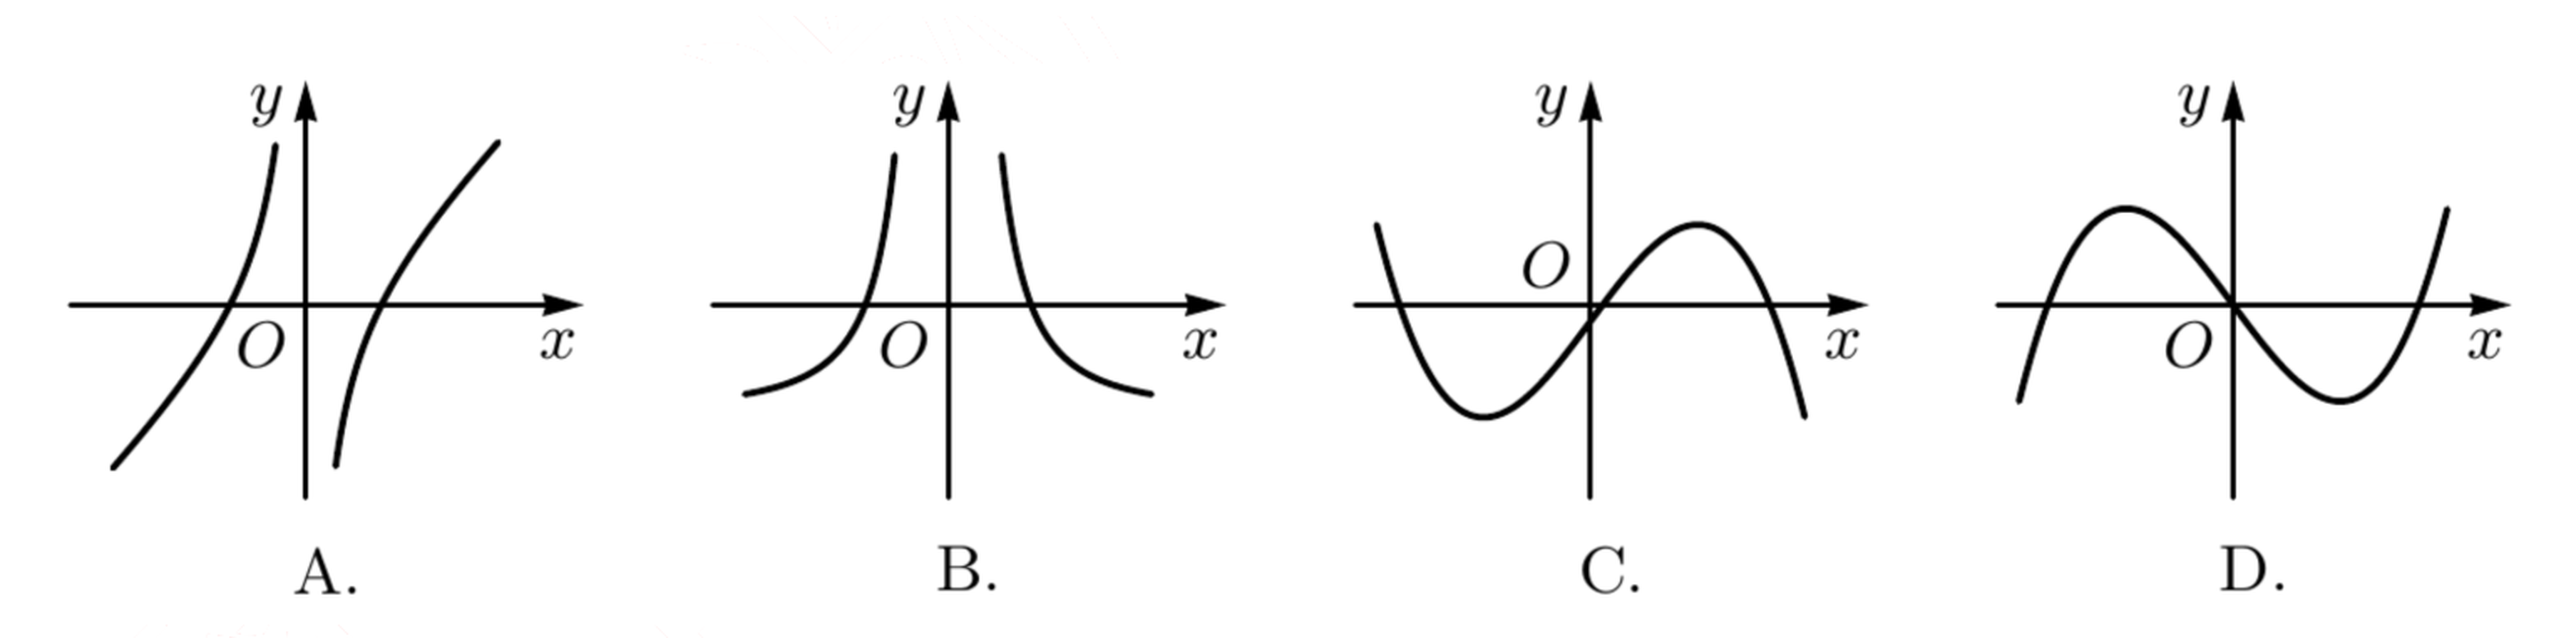
\includegraphics[width=0.90\textwidth]{figures/gao134_q13_options.png}
\end{center}

\ifanswer
\solbegin
\step{$f(x)$ 为偶函数，$g(x)$ 为奇函数，因此 $f(x)g(x)$ 为奇函数，排除 B.}
\step{又 $x=0$ 不在乘积函数的定义域内，其图象在 $y$ 轴上没有点，排除 C、D，}
\step{故选 $A$.}
\solend
\fi

\item 设全集为自然数集 $\N$，$E=\{x\mid x=2n,n\in\N\}$，$F=\{x\mid x=4n,n\in\N\}$，那么集合 $\N$ 可以表示成\mbox{（\quad）}

\keepwithprev
A. $E\cap F$\qquad\qquad B. $\overline{E}\cup F$\qquad\qquad C. $\overline{F}\cup E$\qquad\qquad D. $\overline{E}\cap\overline{F}$

\ifanswer
\solbegin
\step{$F\subseteq E$，所以 $\overline{F}\cup E=\N$，故选 $C$.}
\solend
\fi

\item 已知函数 $y=f(x)$，其中 $f(x)=x^2+bx$，则“$b<0$”是“$f(f(x))$ 的最小值与 $f(x)$ 的最小值相等”的\mbox{（\quad）}

\keepwithprev
A. 充分非必要条件\qquad\qquad B. 必要非充分条件

C. 充分必要条件\qquad\qquad D. 既非充分又非必要条件

\ifanswer
\solbegin
\step{$f(x)=\left(x+\dfrac b2\right)^2-\dfrac{b^2}4$，最小值为 $-\dfrac{b^2}4$，值域为 $\left[-\dfrac{b^2}4,+\infty\right)$.}
\step{当 $b<0$ 时，$-\dfrac b2>0\geqslant-\dfrac{b^2}4$，存在 $x$ 使 $f(x)=-\dfrac b2$，}
\step{从而 $f(f(x))$ 的最小值也为 $-\dfrac{b^2}4$，充分性成立.}
\step{当 $b=0$ 时，$f(x)=x^2$，$f(f(x))=x^4$，两者最小值均为 $0$，必要性不成立.}
\step{故选 $A$.}
\solend
\fi

\item 已知 $a,b,c\in\R$，若存在常数 $M>0$，使得 $a^2+b^2+c^2<M$，则称 $(a,b,c)$ 是有界数组. 对以下两个命题：

①若 $\lvert a^2+b+c\rvert+\lvert a^2+b-c\rvert\leqslant1$，则 $(a,b,c)$ 是有界数组；

②若 $\lvert a^2+b+c\rvert+\lvert a+b^2-c\rvert\leqslant1$，则 $(a,b,c)$ 是有界数组.% ②第二项为 \lvert a+b^2-c\rvert，与①刻意不同，照录

下列判断正确的是\mbox{（\quad）}

\keepwithprev
A. ①和②均为真命题\qquad\qquad B. ①和②均为假命题

C. ①为真命题，②为假命题\qquad D. ①为假命题，②为真命题

\ifanswer
\solbegin
\step{①取 $a=t,b=-t^2,c=0$，条件左端为 $0$，而 $a^2+b^2+c^2=t^2+t^4$ 可任意大，}
\step{故①为假命题.}
\step{②由条件，$a^2+a+b^2+b\leqslant\lvert a^2+b+c\rvert+\lvert a+b^2-c\rvert\leqslant1$.}
\step{由 $(a+1)^2+(b+1)^2\geqslant0$，得 $a^2+b^2\leqslant2(a^2+a+b^2+b)+2\leqslant4$.}
\step{又 $\lvert c\rvert\leqslant\lvert a^2+b+c\rvert+a^2+\lvert b\rvert\leqslant1+4+2=7$，故 $a^2+b^2+c^2\leqslant53<54$，}
\step{可取 $M=54$，故②为真命题.}
\step{故选 $D$.}
\solend
\fi

\end{enumerate}

\bigsec{三、解答题}

\begin{enumerate}
\setcounter{enumi}{16}

\item 已知不等式 $x^2-ax-b<0$ 的解集为 $A$，不等式 $\dfrac{3-2x}{x-1}<0$ 的解集为 $B$.

(1) 若 $a=5$，$b=-6$，求 $A\cap\overline{B}$；

(2) 若 $b=2a^2$，且 $A\cup B=B$，求实数 $a$ 的取值范围.

\ifanswer
\solbegin
\step{(1) 不等式 $\dfrac{3-2x}{x-1}<0$ 等价于 $x<1$ 或 $x>\dfrac32$，}
\step{所以 $B=(-\infty,1)\cup\left(\dfrac32,+\infty\right)$，$\overline{B}=\left[1,\dfrac32\right]$，}
\step{由 $x^2-5x+6=(x-2)(x-3)<0$，得 $A=(2,3)$，因此 $A\cap\overline{B}=\varnothing$.}
\step{(2) $A\cup B=B\Leftrightarrow A\subseteq B$，且 $x^2-ax-2a^2=(x-2a)(x+a)$，}
\step{当 $a=0$ 时，$A=\varnothing$，满足条件.}
\step{当 $a>0$ 时，$A=(-a,2a)$，$-a<0<1$，$A\subseteq B\Leftrightarrow2a\leqslant1$，得 $0<a\leqslant\dfrac12$.}
\step{当 $a<0$ 时，$A=(2a,-a)$，$2a<0<1$，$A\subseteq B\Leftrightarrow-a\leqslant1$，}
\step{得 $-1\leqslant a<0$.}
\step{因此 $a$ 的取值范围为 $\left[-1,\dfrac12\right]$.}
\solend
\fi

\item 为了在夏季降温和冬季供暖时减少能源损耗，房屋的屋顶和外墙需要建造隔热层. 某幢建筑物要建造可使用 $30$ 年的隔热层，每厘米厚的隔热层建造成本为 $9$ 万元. 该建筑物每年的能源消耗费用 $C$（万元）与隔热层厚度 $x$（cm）满足如下关系式：$C=\dfrac{k}{3x+5}$（$0\leqslant x\leqslant10$）. 若不建隔热层，每年能源消耗费用为 $8$ 万元. 设 $y$（万元）为隔热层建造费用与 $30$ 年的能源消耗费用之和.

(1) 求 $k$ 的值及 $y$ 的表达式；

(2) 隔热层修建多厚时，总费用 $y$ 最小？并求最小值.

\ifanswer
\solbegin
\step{(1) 不建隔热层时 $x=0$，$C=8$，所以 $\dfrac k5=8$，得 $k=40$.}
\step{隔热层建造费用为 $9x$ 万元，$30$ 年的能源消耗费用为 $30\times\dfrac{40}{3x+5}$ 万元.}
\step{因此 $y=9x+\dfrac{1200}{3x+5}$，$0\leqslant x\leqslant10$.}
\step{(2) 令 $t=3x+5$，则 $5\leqslant t\leqslant35$，且 $y=3t+\dfrac{1200}{t}-15$，}
\step{因为 $t>0$，由基本不等式得 $y\geqslant2\sqrt{3t\cdot\dfrac{1200}{t}}-15=105$，}
\step{当且仅当 $3t=\dfrac{1200}{t}$，即 $t=20$时取等号，此时 $x=5\in[0,10]$，}% 原卷"20"与"时"之间未留空，照录
\step{所以隔热层厚度为 $5$ cm 时，总费用最小，最小值为 $105$ 万元.}
\solend
\fi

\item 已知 $f(x)=ax^2+\dfrac1x$，其中 $a$ 为常数.

(1) 若 $a\in(1,3)$，判断函数 $y=f(x)$ 在 $[1,2]$ 上的单调性，并用定义证明；

(2) 求函数 $y=f(x)-x-\dfrac1x$ 在 $[1,2]$ 上的最大值 $g(a)$.

\ifanswer
\solbegin
\step{(1) 任取 $x_1,x_2\in[1,2]$，且 $x_1<x_2$，}
\step{则 $f(x_2)-f(x_1)=(x_2-x_1)\left[a(x_1+x_2)-\dfrac1{x_1x_2}\right]$，}
\step{由 $a>1$，$x_1+x_2\geqslant2$，$x_1x_2\geqslant1$，得 $a(x_1+x_2)-\dfrac1{x_1x_2}>2-1>0$，}
\step{因此 $f(x_2)>f(x_1)$，$f(x)$ 在 $[1,2]$ 上为严格增函数.}
\step{(2) 令 $h(x)=f(x)-x-\dfrac1x=ax^2-x$，其中 $x\in[1,2]$.}
\step{若 $a=0$，则 $h(x)=-x$，所以 $h(x)_{max}=h(1)=-1$；}
\step{若 $a<0$，二次函数的图象的对称轴为 $x=\dfrac1{2a}<0$，}
\step{所以 $y=h(x)$ 在 $[1,2]$ 上是严格减函数，所以 $h(x)_{max}=h(1)=a-1$；}
\step{若 $a>0$ 且 $\dfrac1{2a}>\dfrac32$，即 $0<a<\dfrac13$ 时，$h(x)_{max}=h(1)=a-1$.}
\step{若 $a>0$ 且 $\dfrac1{2a}\leqslant\dfrac32$，即 $a\geqslant\dfrac13$ 时，$h(x)_{max}=h(2)=4a-2$.}
\step{综上所述，$g(a)=\begin{cases}a-1,a<\dfrac13\\4a-2,a\geqslant\dfrac13\end{cases}$.}
\solend
\fi

\item 已知 $f(x)=\dfrac{ax^2+1}{bx+c}$（$a,b,c\in\Z$）.

(1) 若函数 $y=f(x)$ 是奇函数，且 $f(1)=2$，$f(2)<3$，求 $a,b,c$ 的值；

(2) 若函数 $y=f(x)$ 是偶函数，且 $ac<0$，$f(2a^2+a+1)<f(-3a^2+2a-1)$，求 $a$ 的值；

(3) 若 $b=a+c^2$，且满足不等式 $\lvert f(x)\rvert\geqslant1$ 的 $x$ 的最大值为 $0$，求 $c$ 的值.

\ifanswer
\solbegin
\step{(1) 由 $f(-x)=-f(x)$，交叉相乘得 $2c(ax^2+1)=0$ 恒成立，}
\step{因此 $c=0$，$b\neq0$.}
\step{由 $f(1)=2$，得 $a+1=2b$，}
\step{于是 $f(2)=\dfrac{4a+1}{2b}=4-\dfrac3{2b}<3\Leftrightarrow0<b<\dfrac32$，}
\step{因为 $b\in\Z$，所以 $b=1$，进而 $a=1$，$c=0$.}
\step{(2) 由 $f(-x)=f(x)$，交叉相乘得 $2bx(ax^2+1)=0$ 恒成立，因此 $b=0$.}
\step{此时 $f(x)=\dfrac ac x^2+\dfrac1c$，且 $\dfrac ac<0$.}
\step{设 $u=2a^2+a+1$，$v=-3a^2+2a-1$.}
\step{方程 $2a^2+a+1=0$ 与 $3a^2-2a+1=0$ 的判别式分别为 $-7$ 与 $-8$，}
\step{都小于 $0$，所以 $u>0$，$v<0$.}
\step{于是 $f(u)<f(v)\Leftrightarrow u^2>v^2\Leftrightarrow u>-v\Leftrightarrow-a^2+3a>0\Leftrightarrow0<a<3$，}
\step{因为 $a\in\Z$，所以 $a=1$ 或 $a=2$.}
\step{(3) 因为解集的最大值为 $0$，所以 $f(0)$ 有定义且 $\lvert f(0)\rvert\geqslant1$，}
\step{即 $c\neq0$，$\left\lvert\dfrac1c\right\rvert\geqslant1$，结合 $c\in\Z$，得 $c=\pm1$，从而 $b=a+1$.}
\step{当 $x=2$ 时，分母 $2a+2+c$ 为奇数，必不为 $0$；}
\step{又因为 $2>0$，必须有 $\lvert f(2)\rvert<1\Leftrightarrow\lvert4a+1\rvert<\lvert2a+2+c\rvert$，}
\step{若 $c=-1$，则 $(4a+1)^2<(2a+1)^2\Leftrightarrow4a(3a+1)<0\Leftrightarrow-\dfrac13<a<0$，}
\step{不存在满足条件的整数 $a$.}
\step{若 $c=1$，则 $(4a+1)^2<(2a+3)^2\Leftrightarrow4(3a+2)(a-1)<0\Leftrightarrow-\dfrac23<a<1$，}
\step{所以 $a=0$，$b=1$，此时 $f(x)=\dfrac1{x+1}$，}
\step{且 $\lvert f(x)\rvert\geqslant1\Leftrightarrow0<\lvert x+1\rvert\leqslant1\Leftrightarrow x\in[-2,-1)\cup(-1,0]$，}
\step{解集的最大值确为 $0$，因此 $c=1$.}
\solend
\fi

\item 已知函数 $y=f(x)$ 的定义域为 $\R$，且当 $x>0$ 时，$f(x)=\dfrac1{x+1}$. 对任意 $x_0\in\R$，定义集合 $D(x_0)=\{d\mid f(x_0+d)>f(x_0)\}$.

(1) 若当 $x\leqslant0$ 时，$f(x)=-2x+1$，求函数 $y=f(x)$ 的值域；

(2) 若 $y=f(x)$ 是偶函数，且 $f(0)=1$，求证：$D(-2)=\{-d\mid d\in D(2)\}$；

(3) 若 $y=f(x)$ 是奇函数，且 $x_1x_2\neq0$，求证：“$f(x_1)\leqslant f(x_2)$”的充要条件是\!\mbox{“$D(x_2)\subseteq D(x_1)$”}.

\ifanswer
\solbegin
\step{(1) 当 $x>0$ 时，$0<f(x)<1$；当 $x\leqslant0$ 时，$f(x)=-2x+1\geqslant1$.}
\step{函数的值域为 $(0,1)\cup[1,+\infty)=(0,+\infty)$.}
\step{(2) 由 $f(x)$ 是偶函数及 $f(0)=1$，得 $f(x)=\dfrac1{1+\lvert x\rvert}$，且 $f(2)=f(-2)=\dfrac13$.}
\stepm{法一：}{$D(2)=\left\{d\mid\dfrac1{1+\lvert2+d\rvert}>\dfrac13\right\}=\{d\mid\lvert2+d\rvert<2\}=(-4,0)$，}
\step{$D(-2)=\left\{d\mid\dfrac1{1+\lvert-2+d\rvert}>\dfrac13\right\}=\{d\mid\lvert-2+d\rvert<2\}=(0,4)$，}
\step{因此 $\{-d\mid d\in D(2)\}=(0,4)=D(-2)$.}
\stepm{法二：}{任取 $d\in D(-2)$，由定义得 $f(-2+d)>f(-2)$.}
\step{因为 $y=f(x)$ 是偶函数，所以对任意的实数 $x$，有 $f(-x)=f(x)$，}
\step{因此 $f(-2+d)=f(-(-2+d))=f(2-d)$，且 $f(-2)=f(2)$.}
\step{所以不等式 $f(-2+d)>f(-2)$ 等价于 $f(2-d)>f(2)$，}
\step{这恰好是 $-d\in D(2)$ 的定义，}
\step{所以 $d\in D(-2)\Leftrightarrow-d\in D(2)$，故 $D(-2)=\{-d\mid d\in D(2)\}$.}
\step{(3) 由 $f(x)$ 是奇函数，得 $f(0)=0$；}
\step{当 $x<0$ 时，$f(x)=-f(-x)=-\dfrac1{1-x}=\dfrac1{x-1}$；}
\step{所以 $f(x)=\begin{cases}\dfrac1{x-1},&x<0\\0,&x=0;\\\dfrac1{x+1},&x>0\end{cases}$}
% 2026-11-15 回原图订正：原卷 11 页此 cases 块末无句点，本稿初转顺手补了西文句点，今删去（Q19 08 页同类块末有句点，照录保留）。
\step{当 $x_0<0$ 时，$D(x_0)=\{d\mid f(x_0+d)>f(x_0)\}=(-\infty,0)\cup[-x_0,+\infty)$，}
\step{当 $x_0=0$ 时，$D(0)=\{d\mid f(0+d)>f(0)\}=(0,+\infty)$，}
\step{当 $x_0>0$ 时，$D(x_0)=\{d\mid f(x_0+d)>f(x_0)\}=(-x_0,0)$.}
\stepm{先证明必要性.}{若 $f(x_1)\leqslant f(x_2)$，仅需讨论三类情形：}
\step{若 $x_2\leqslant x_1<0$，}
\step{则 $D(x_1)=(-\infty,0)\cup[-x_1,+\infty),D(x_2)=(-\infty,0)\cup[-x_2,+\infty)$，}
\step{故 $D(x_2)\subseteq D(x_1)$；}
\step{若 $0<x_2\leqslant x_1$，则 $D(x_1)=(-x_1,0),D(x_2)=(-x_2,0)$，}
\step{故 $D(x_2)\subseteq D(x_1)$；}
\step{若 $x_1<0<x_2$，则 $D(x_1)=(-\infty,0)\cup[-x_1,+\infty),D(x_2)=(-x_2,0)$，}
\step{故 $D(x_2)\subseteq D(x_1)$.}
\stepm{再证明充分性.}{若 $D(x_2)\subseteq D(x_1)$，}
\step{若 $x_1<0,x_2<0$，}
\step{则 $D(x_1)=(-\infty,0)\cup[-x_1,+\infty),D(x_2)=(-\infty,0)\cup[-x_2,+\infty)$，}
\step{由 $D(x_2)\subseteq D(x_1)$ 得 $x_2\leqslant x_1$，}
\step{又 $y=f(x)$ 在 $(-\infty,0)$ 上是严格减函数，所以 $f(x_1)\leqslant f(x_2)$；}
\step{若 $x_1>0,x_2>0$，则 $D(x_1)=(-x_1,0),D(x_2)=(-x_2,0)$，}
\step{由 $D(x_2)\subseteq D(x_1)$ 得 $x_2\leqslant x_1$，}
\step{又 $y=f(x)$ 在 $(0,+\infty)$ 上是严格减函数，所以 $f(x_1)\leqslant f(x_2)$；}
\step{若 $x_1<0,x_2>0$，则 $f(x_1)<0<f(x_2)$，结论成立；}
\step{若 $x_1>0,x_2<0$，此时 $D(x_1)=(-x_1,0)$ 中只有负数，}
\step{而 $D(x_2)=(-\infty,0)\cup[-x_2,+\infty)$ 中有正数，$D(x_2)\subseteq D(x_1)$ 不成立.}
\step{综上，“$f(x_1)\leqslant f(x_2)$”的充要条件是“$D(x_2)\subseteq D(x_1)$”.}
\solend
\fi

\end{enumerate}

\end{document}
"
% 紧凑版：xelatex "\def\iscompact{1}% 高一134_华师大二附中_期中.tex
%   —— 高一上数学"2026-2027 年华师大二附中高一上期中"（试卷版/答案版）
% 试卷版：xelatex 高一134_华师大二附中_期中.tex
% 答案版：xelatex "\def\isanswer{1}\input{高一134_华师大二附中_期中.tex}"
% 紧凑版：xelatex "\def\iscompact{1}\input{高一134_华师大二附中_期中.tex}"
%
% ① 原始材料：微信公众号"魔都数学加油站"文章，作者破晓，2026-11-15 18:04 发布；
% 连载"27学年高一134"，原文标题"27学年高一134——2026-2027年上海市华师大二附中高一上期中"；
% 原文链接：https://mp.weixin.qq.com/s/bQlkmlGdCtAlytY331vf3g。
% 正文为 13 张 PNG 页（01、04、06、08、09、10、11、12、13 为 2560x3620；
% 02、03、05、07 为 4762x6735，同一篇各页分辨率不同，逐页按各自分辨率裁图核对），
% 题目下印有【解析】，为讲评版。题目、解析均据原图转录；卷面粉红色水印
% "魔都数学加油站"及公众号页脚未录入。
% 全卷 2 幅插图，均在第 04 页：第 13 题题干 y=f(x)、y=g(x) 两幅函数图象合并裁为
% figures/gao134_q13_graphs.png，第 13 题 A/B/C/D 四幅函数图象选项合并裁为
% figures/gao134_q13_options.png；两图均取原卷 04 页截图 3× LANCZOS 放大、
% 白化粉色水印（只白化浅粉色 R>175 且 G>140 且 B>140 的像素，保留红色标签）。
% 注意：本卷 Q13 四幅选项在原卷排为"一行四幅"（1×4），并非 高一132 第 14 题
% 的 2×2 排布，本稿按原卷 1×4 合并裁为一张，不重排、不用 TikZ 重绘。
%
% 卷首标题：原卷印作"2026-2027 年华师大二附中高一上期中"（公众号标题中的"上海市"
% 卷面标题行没有，本稿照卷面），年份区间按全稿惯例排 en dash；原卷未印副标题，
% 本卷为期中卷、跨集合与常用逻辑用语／不等式／函数三章，按题目内容标为
% "集合与常用逻辑用语、不等式、函数"（与 125／126／128／129／131／132／133 同期中卷口径相同）：
% 集合与逻辑见 Q6、Q10、Q14、Q16、Q17、Q21，不等式见 Q3、Q7、Q9、Q11、Q15、Q18、Q19，
% 函数（函数性质、二分法、奇偶性、基本不等式应用）见 Q4、Q5、Q8、Q12、Q13、Q20。
%
% 题号体例：本卷共 19 题——一、填空题 3—12（10 题）、二、选择题 13—16（4 题）、
% 三、解答题 17—21（5 题）。三节分别 \setcounter{enumi}{2}／{12}／{16}。
% 第 13 页仅为 Q21 (3) 解析续尾，全卷无「四、附加题」。
%
% ② 与原卷的排版差异：
%   ① 原文从第 3 题起，本稿保留原题号（见上"题号体例"）；
%   ② 原卷每题下直接印【解析】，本稿按全稿惯例置于答案版；第 13—16 题答案均在
%      解析末句"故选 …"，题干括号内留空、不另提 \ans{}（四题均无独立答案段）；
%      全卷无只印括号内答案、无解析的选择题；
%   ③ 原卷未印副标题，本稿按"知识模块"口径补出；
%   ④ 原卷填空横线按全稿惯例排为 \blankline[4.4em]；选择题括号排 \mbox{（\quad）}、
%      每个选项段前按惯例加 \keepwithprev（Q13 四选项为图，守卫前行为 \begin{center}；
%      Q15、Q16 四选项分两行排，\keepwithprev 只加在 A. 行前）；解答题不留作答区、
%      不加 \anspace（原卷为讲评版，与 129／131／132／133 同）；
%   ⑤ 原卷数集印黑板粗体（Q7／Q11／Q12／Q16／Q21 的 R、Q14／Q20 的 N、Q20 的 Z），
%      按全稿惯例统一排 \R／\N／\Z；绝对值排 \lvert…\rvert，集合描述竖线排 \mid；不等号按全稿惯例排
%      \leqslant／\geqslant；补集照原卷上划线排 \overline{B}、\overline{E}、\overline{F}；
%   ⑥ 子题标号 (1)(2)(3) 与括注原卷均用半角括号，照录（与 131／132／133 同）；
%      圈数字 ①② 照录；原卷 Q21 (2) 解析"法一：""法二："与 Q21 (3) 解析
%      "先证明必要性.""再证明充分性."四处标签印红色加粗，按 高一53／108／133 成例排
%      \stepm{法一：}／\stepm{法二：}／\stepm{先证明必要性.}／\stepm{再证明充分性.}
%      （加粗着色、不引入红色，不动 common.sty）；Q8 解析"第 1 步：""第 2 步：""
%      "第 3 步："原卷印黑色常规宋体（非红非粗），照录为普通 \step 行内文字；
%   ⑦ 数学式内半角逗号照录（如 Q6 $A=\{0,1,2,3\}$、Q14 $x=2n,n\in\N$、
%      Q16 $a,b,c\in\R$ 与 $a=t,b=-t^2,c=0$、Q19 $x_1,x_2\in[1,2]$、
%      Q20 $a,b,c\in\Z$、Q21 $x_1<0,x_2<0$ 与 $D(x_1)=(-x_1,0),D(x_2)=(-x_2,0)$）；
%      原卷行末全角句点按全稿惯例从宽排西文句点；cases 块末的句点逐处照录：
%      Q19 解析（08 页）块末原卷有句点照录、Q21 (3) 解析（11 页）块末原卷无句点不补，
%      两处原卷自身不统一（2026-11-15 回原图核对，本稿初转曾顺手补句点，已删去）；
%   ⑧ 原卷 Q8 解析跨 01—02 页、Q10 解析跨 02—03 页、Q12 解析跨 03—04 页、
%      Q16 解析跨 05—06 页、Q17 解析跨 06—07 页、Q20 解析跨 08—10 页、
%      Q21 解析跨 10—13 页，本稿按题合并连续排版；末页第 13 页为
%      Q21 (3) 解析续尾与"综上"一句，按实际印刷行单列；
%   ⑨ 题干中的中文弯引号按原卷照录（Q10 研究问题、Q15 条件、Q21 (3) 充要条件），
%      注释内一律 ASCII 引号。
%
% 判别式字形：全卷仅 Q9 解析末行出现一处判别式记号
%   "两值均满足 $\Delta=p^2-4p=18\mp12\sqrt2>0$"，逐处放大核对，原卷印高三角
%   $\Delta$（等腰、高，实测高宽比约 1.14），照录 \Delta；卷内无扁三角 \triangle，
%   与 高一132 同题排 $\triangle$、高一133 部分判别式排 $\triangle$ 均不同。
%
% 子集符号：Q6 题干 $C\subseteq A$、$C\subseteq B$ 与解析 $C\subseteq A\cap B$、
%   Q14 解析 $F\subseteq E$、Q17 解析 $A\subseteq B$、Q21 题干与解析各处的
%   $D(x_2)\subseteq D(x_1)$，全部印带下划线的 $\subseteq$，逐处放大核对，
%   照录 \subseteq；全卷未出现单线 \subset。
%
% 原卷存疑照录（均照录未改，正文对应处另有 % 注）：
%   第 6 题题干集合 $A=\{0,1,2,3\}$ 三个逗号后不留空，紧邻的 $B=\{0,2,4,5\}$
%      三个逗号后却留空，同卷同一行两集合排字不一，照录其逗号均为半角；
%   第 16 题命题②作 $\lvert a^2+b+c\rvert+\lvert a+b^2-c\rvert\leqslant1$，
%      与命题①第二项 $\lvert a^2+b-c\rvert$ 不同（①无 $b$ 的平方、②有），
%      两命题刻意不同，照录；解析"②由条件，$a^2+a+b^2+b\leqslant\cdots$"
%      由两项相加直接得到，照录；
%   第 18 题 (2) 解析"即 $t=20$时取等号"中"20"与"时"之间原卷未留空，照录；
%   第 19 题解析 $h(x)_{max}$ 的"max"下标三处字形不一（斜体／正体混排），照录；
%   第 20 题 (1)(2) 解析"由 $f(-x)=-f(x)$，交叉相乘得……"与"由 $f(-x)=f(x)$，
%      交叉相乘得……"两处措辞照录；
%   第 21 题 (2) 原卷并存"法一"（集合计算）与"法二"（定义推证）两套证明，照录不删。
%
% 行数复核：逐题数 \step/\stepm 条数，合计 134 条（Q3：2；Q4：1；Q5：1；Q6：1；
% Q7：2；Q8：4；Q9：3；Q10：4；Q11：5；Q12：8；Q13：3；Q14：1；Q15：5；
% Q16：7；Q17：9；Q18：7；Q19：11；Q20：22；Q21：38），与原卷印刷行逐题相等
% （cases 块作一个印刷行计）。第 13—16 题答案在解析末句，括号内留空、不另提 \ans{}；
% 第 21 题四条 \stepm 计入 38 条内。
%
\documentclass[a4paper,11pt]{article}
\usepackage{common}

\begin{document}

\examtitlest[3]{2026--2027 年华师大二附中高一上期中}{集合与常用逻辑用语、不等式、函数}

\bigsec{一、填空题}

\begin{enumerate}
\setcounter{enumi}{2}

\item 不等式 $\lvert 2x+1\rvert\geqslant3$ 的解集为\blankline[4.4em].

\ifanswer
\solbegin
\step{$\lvert 2x+1\rvert\geqslant3\Leftrightarrow 2x+1\leqslant-3$ 或 $2x+1\geqslant3\Leftrightarrow x\leqslant-2$ 或 $x\geqslant1$，}
\step{故解集为 $(-\infty,-2]\cup[1,+\infty)$.}
\solend
\fi

\item 函数 $y=\sqrt{x+1}+\dfrac1x$ 的定义域为\blankline[4.4em].

\ifanswer
\solbegin
\step{$x+1\geqslant0$ 且 $x\neq0$，得定义域为 $[-1,0)\cup(0,+\infty)$.}
\solend
\fi

\item 已知等式 $3x^2-4x-2=a(x-1)^2+b(x-1)+c$ 恒成立，其中 $a$、$b$、$c$ 为常数，则 $a-b+c=$\blankline[4.4em].

\ifanswer
\solbegin
\step{令 $x=0$，得 $a-b+c=-2$.}
\solend
\fi

\item 已知集合 $A=\{0,1,2,3\}$，$B=\{0,2,4,5\}$，$C\subseteq A$，$C\subseteq B$，符合条件的集合 $C$ 有\blankline[4.4em]个.% 原卷 A 的逗号后不留空、B 的逗号后留空，排字不一，照录

\ifanswer
\solbegin
\step{$C\subseteq A\cap B=\{0,2\}$，所以符合条件的集合 $C$ 有 $2^2=4$ 个.}
\solend
\fi

\item 设 $a$、$b\in\R$，且 $a^2+4b^2=2$，则 $ab$ 的最大值为\blankline[4.4em].

\ifanswer
\solbegin
\step{$(a-2b)^2=a^2+4b^2-4ab=2-4ab\geqslant0$，得 $ab\leqslant\dfrac12$，}
\step{当且仅当 $a=2b=\pm1$ 时取等号，故 $ab$ 的最大值为 $\dfrac12$.}
\solend
\fi

\item 已知函数 $y=x(13-2x)^2-140$，用二分法求函数在区间 $(3,4)$ 上的零点时，第 3 步应计算 $x=$\blankline[4.4em]的函数值.

\ifanswer
\solbegin
\step{记 $f(x)=x(13-2x)^2-140$，则 $f(3)=7>0$，$f(4)=-40<0$.}
\step{第 1 步：$f\left(\dfrac72\right)=-14<0$，区间缩小为 $\left(3,\dfrac72\right)$.}
\step{第 2 步：$f\left(\dfrac{13}4\right)=-\dfrac{43}{16}<0$，区间缩小为 $\left(3,\dfrac{13}4\right)$.}
\step{第 3 步：应计算 $x=\dfrac{3+\frac{13}4}2=\dfrac{25}8$ 的函数值.}
\solend
\fi

\item 已知一元二次方程 $x^2+px+p=0$ 的两个实根分别为 $x_1$、$x_2$，且 $x_1^2x_2+x_2^2x_1=-18$，则 $p=$\blankline[4.4em].% 判别式 \Delta 高三角，逐处放大核对

\ifanswer
\solbegin
\step{由韦达定理，$x_1+x_2=-p$，$x_1x_2=p$，}
\step{则 $x_1^2x_2+x_2^2x_1=x_1x_2(x_1+x_2)=-p^2=-18\Rightarrow p=\pm3\sqrt2$，}
\step{两值均满足 $\Delta=p^2-4p=18\mp12\sqrt2>0$，故 $p=\pm3\sqrt2$.}
\solend
\fi

\item 研究问题：“已知关于 $x$ 的不等式 $ax^2-bx+c>0$ 的解集为 $(1,2)$，解关于 $x$ 的不等式 $cx^2-bx+a>0$”，有如下解法：

解：由 $ax^2-bx+c>0\Rightarrow a-b\left(\dfrac1x\right)+c\left(\dfrac1x\right)^2>0$，令 $y=\dfrac1x$，则 $y\in\left(\dfrac12,1\right)$，

所以不等式 $cx^2-bx+a>0$ 的解集为 $\left(\dfrac12,1\right)$.

参考上述解法，已知关于 $x$ 的不等式 $\dfrac{k}{x+a}+\dfrac{x+b}{x+c}<0$ 的解集为 $(-3,-1)\cup(2,4)$，则关于 $x$ 的不等式 $\dfrac{kx}{ax-1}+\dfrac{bx-1}{cx-1}<0$ 的解集为\blankline[4.4em].

\ifanswer
\solbegin
\step{当 $x=0$ 时，所求不等式左端为 $1$，不满足不等式.}
\step{当 $x\neq0$ 时，两个分式的分子、分母同除以 $x$，得 $\dfrac{k}{a-\frac1x}+\dfrac{b-\frac1x}{c-\frac1x}<0$.}
\step{令 $t=-\dfrac1x$，则所求不等式化为 $\dfrac{k}{t+a}+\dfrac{t+b}{t+c}<0$，即 $-\dfrac1x\in(-3,-1)\cup(2,4)$，}
\step{解得 $x\in\left(-\dfrac12,-\dfrac14\right)\cup\left(\dfrac13,1\right)$.}
\solend
\fi

\item 已知 $a\in(0,+\infty)$，若对任意的 $x\in(0,+\infty)$，均有 $\lvert x^2-a\rvert+\lvert x+b\rvert=\lvert x^2+x-a+b\rvert$，则 $a^2-b^2$ 的最小值为\blankline[4.4em].

\ifanswer
\solbegin
\step{原等式成立的充要条件是 $(x^2-a)(x+b)\geqslant0$.}
\step{当 $0<x<\sqrt a$ 时须有 $x+b\leqslant0$；当 $x>\sqrt a$ 时须有 $x+b\geqslant0$，因此 $b=-\sqrt a$.}
\step{此时 $(x^2-a)(x+b)=(x+\sqrt a)(x-\sqrt a)^2\geqslant0$，满足题意.}
\step{$a^2-b^2=a^2-a=\left(a-\dfrac12\right)^2-\dfrac14\geqslant-\dfrac14$，}
\step{当 $a=\dfrac12$，$b=-\dfrac{\sqrt2}2$ 时取等号，最小值为 $-\dfrac14$.}
\solend
\fi

\item 已知函数 $y=f(x)$ 在 $\R$ 上是严格增函数，当 $x\neq0$ 且 $f(x)\neq0$ 时，满足 $f(x)\cdot f\left[\dfrac1{f(x)}+\dfrac1x\right]=1$，则 $f(1)=$\blankline[4.4em].

\ifanswer
\solbegin
\step{当 $xf(x)>0$ 时，记 $t=\dfrac1{f(x)}+\dfrac1x\neq0$，则 $f(t)=\dfrac1{f(x)}\neq0$.}
\step{将 $t$ 代入题设，得 $f\left(f(x)+\dfrac1t\right)=f(x)$，严格增性给出 $f(x)+\dfrac1t=x$，}
\step{化简得 $f(x)^2+xf(x)-x^2=0$，由 $\dfrac{f(x)}x>0$ 得 $f(x)=\dfrac{\sqrt5-1}2x$.}
\step{设 $a=f(0)$，若 $a>0$，则 $f(a)>f(0)=a>0$；}
\step{若 $a<0$，则 $f(a)<f(0)=a<0$.}
\step{两种情形都有 $af(a)>0$ 且 $\dfrac{f(a)}a>1$，与上式 $\dfrac{f(a)}a=\dfrac{\sqrt5-1}2<1$ 矛盾，}
\step{因此 $f(0)=0$.}
\step{于是 $f(1)>0$，代入上式得 $f(1)=\dfrac{\sqrt5-1}2$.}
\solend
\fi

\end{enumerate}

% 第 13 题是"节标题 + 题干 + 两幅图 + 四幅选项图"约 15cm 的整块，
% 守卫只放在 \bigsec 之前；若再在 \item 之前放第二枚，会在标题已印出后才触发换页，
% 把题目推走、留下孤立节标题（切页审计 B 类）。高度须覆盖整块。
\needvspace{16cm}
\bigsec{二、选择题}

\begin{enumerate}
\setcounter{enumi}{12}

\item 已知函数 $y=f(x)$ 与 $y=g(x)$ 的图象如图所示，则函数 $y=f(x)\cdot g(x)$ 的图象可能是\mbox{（\quad）}

\keepwithprev
\begin{center}
% 题干 y=f(x)、y=g(x) 两幅函数图象取原卷 04 页截图去粉色水印，按原卷左右排布合并为一张
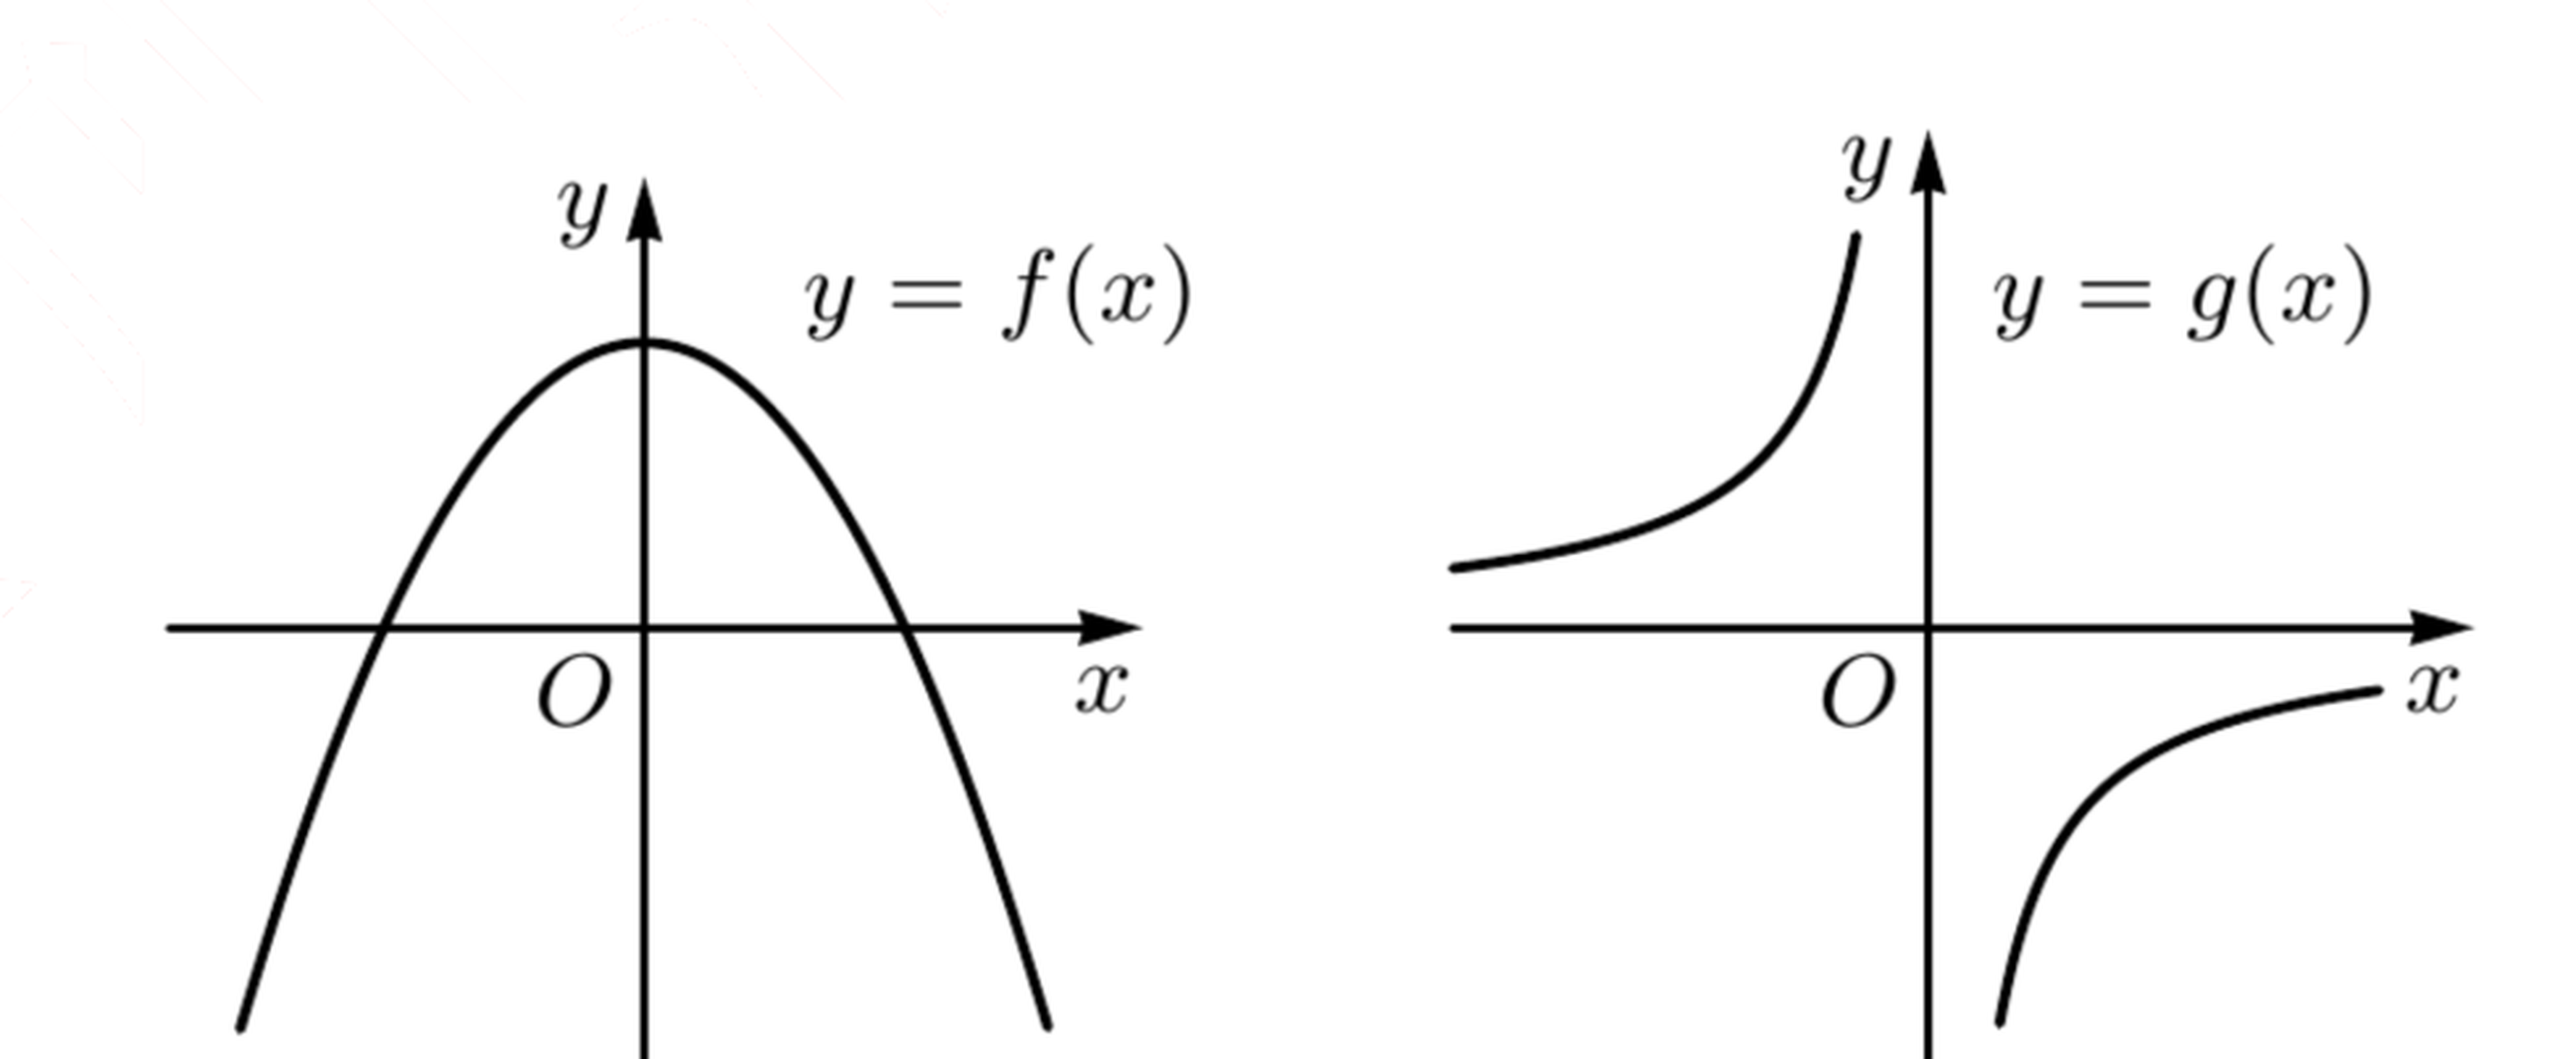
\includegraphics[width=0.72\textwidth]{figures/gao134_q13_graphs.png}\\[0.6em]
% A/B/C/D 四幅函数图象选项取原卷 04 页截图去粉色水印，按原卷一行四幅排布合并为一张
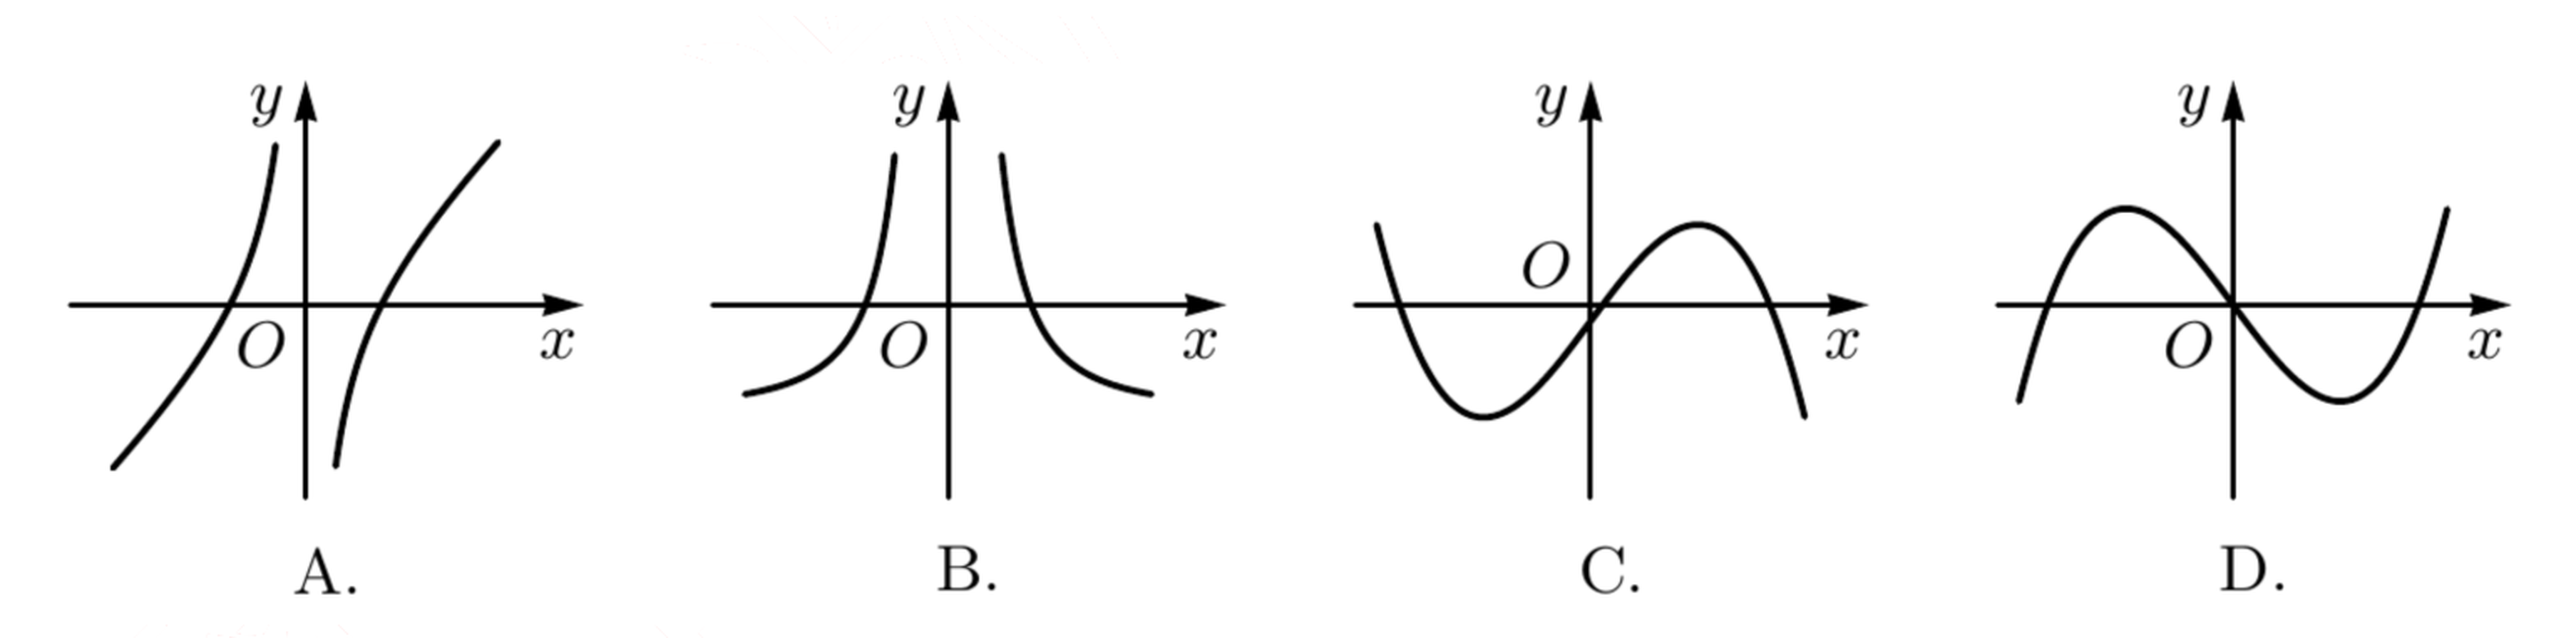
\includegraphics[width=0.90\textwidth]{figures/gao134_q13_options.png}
\end{center}

\ifanswer
\solbegin
\step{$f(x)$ 为偶函数，$g(x)$ 为奇函数，因此 $f(x)g(x)$ 为奇函数，排除 B.}
\step{又 $x=0$ 不在乘积函数的定义域内，其图象在 $y$ 轴上没有点，排除 C、D，}
\step{故选 $A$.}
\solend
\fi

\item 设全集为自然数集 $\N$，$E=\{x\mid x=2n,n\in\N\}$，$F=\{x\mid x=4n,n\in\N\}$，那么集合 $\N$ 可以表示成\mbox{（\quad）}

\keepwithprev
A. $E\cap F$\qquad\qquad B. $\overline{E}\cup F$\qquad\qquad C. $\overline{F}\cup E$\qquad\qquad D. $\overline{E}\cap\overline{F}$

\ifanswer
\solbegin
\step{$F\subseteq E$，所以 $\overline{F}\cup E=\N$，故选 $C$.}
\solend
\fi

\item 已知函数 $y=f(x)$，其中 $f(x)=x^2+bx$，则“$b<0$”是“$f(f(x))$ 的最小值与 $f(x)$ 的最小值相等”的\mbox{（\quad）}

\keepwithprev
A. 充分非必要条件\qquad\qquad B. 必要非充分条件

C. 充分必要条件\qquad\qquad D. 既非充分又非必要条件

\ifanswer
\solbegin
\step{$f(x)=\left(x+\dfrac b2\right)^2-\dfrac{b^2}4$，最小值为 $-\dfrac{b^2}4$，值域为 $\left[-\dfrac{b^2}4,+\infty\right)$.}
\step{当 $b<0$ 时，$-\dfrac b2>0\geqslant-\dfrac{b^2}4$，存在 $x$ 使 $f(x)=-\dfrac b2$，}
\step{从而 $f(f(x))$ 的最小值也为 $-\dfrac{b^2}4$，充分性成立.}
\step{当 $b=0$ 时，$f(x)=x^2$，$f(f(x))=x^4$，两者最小值均为 $0$，必要性不成立.}
\step{故选 $A$.}
\solend
\fi

\item 已知 $a,b,c\in\R$，若存在常数 $M>0$，使得 $a^2+b^2+c^2<M$，则称 $(a,b,c)$ 是有界数组. 对以下两个命题：

①若 $\lvert a^2+b+c\rvert+\lvert a^2+b-c\rvert\leqslant1$，则 $(a,b,c)$ 是有界数组；

②若 $\lvert a^2+b+c\rvert+\lvert a+b^2-c\rvert\leqslant1$，则 $(a,b,c)$ 是有界数组.% ②第二项为 \lvert a+b^2-c\rvert，与①刻意不同，照录

下列判断正确的是\mbox{（\quad）}

\keepwithprev
A. ①和②均为真命题\qquad\qquad B. ①和②均为假命题

C. ①为真命题，②为假命题\qquad D. ①为假命题，②为真命题

\ifanswer
\solbegin
\step{①取 $a=t,b=-t^2,c=0$，条件左端为 $0$，而 $a^2+b^2+c^2=t^2+t^4$ 可任意大，}
\step{故①为假命题.}
\step{②由条件，$a^2+a+b^2+b\leqslant\lvert a^2+b+c\rvert+\lvert a+b^2-c\rvert\leqslant1$.}
\step{由 $(a+1)^2+(b+1)^2\geqslant0$，得 $a^2+b^2\leqslant2(a^2+a+b^2+b)+2\leqslant4$.}
\step{又 $\lvert c\rvert\leqslant\lvert a^2+b+c\rvert+a^2+\lvert b\rvert\leqslant1+4+2=7$，故 $a^2+b^2+c^2\leqslant53<54$，}
\step{可取 $M=54$，故②为真命题.}
\step{故选 $D$.}
\solend
\fi

\end{enumerate}

\bigsec{三、解答题}

\begin{enumerate}
\setcounter{enumi}{16}

\item 已知不等式 $x^2-ax-b<0$ 的解集为 $A$，不等式 $\dfrac{3-2x}{x-1}<0$ 的解集为 $B$.

(1) 若 $a=5$，$b=-6$，求 $A\cap\overline{B}$；

(2) 若 $b=2a^2$，且 $A\cup B=B$，求实数 $a$ 的取值范围.

\ifanswer
\solbegin
\step{(1) 不等式 $\dfrac{3-2x}{x-1}<0$ 等价于 $x<1$ 或 $x>\dfrac32$，}
\step{所以 $B=(-\infty,1)\cup\left(\dfrac32,+\infty\right)$，$\overline{B}=\left[1,\dfrac32\right]$，}
\step{由 $x^2-5x+6=(x-2)(x-3)<0$，得 $A=(2,3)$，因此 $A\cap\overline{B}=\varnothing$.}
\step{(2) $A\cup B=B\Leftrightarrow A\subseteq B$，且 $x^2-ax-2a^2=(x-2a)(x+a)$，}
\step{当 $a=0$ 时，$A=\varnothing$，满足条件.}
\step{当 $a>0$ 时，$A=(-a,2a)$，$-a<0<1$，$A\subseteq B\Leftrightarrow2a\leqslant1$，得 $0<a\leqslant\dfrac12$.}
\step{当 $a<0$ 时，$A=(2a,-a)$，$2a<0<1$，$A\subseteq B\Leftrightarrow-a\leqslant1$，}
\step{得 $-1\leqslant a<0$.}
\step{因此 $a$ 的取值范围为 $\left[-1,\dfrac12\right]$.}
\solend
\fi

\item 为了在夏季降温和冬季供暖时减少能源损耗，房屋的屋顶和外墙需要建造隔热层. 某幢建筑物要建造可使用 $30$ 年的隔热层，每厘米厚的隔热层建造成本为 $9$ 万元. 该建筑物每年的能源消耗费用 $C$（万元）与隔热层厚度 $x$（cm）满足如下关系式：$C=\dfrac{k}{3x+5}$（$0\leqslant x\leqslant10$）. 若不建隔热层，每年能源消耗费用为 $8$ 万元. 设 $y$（万元）为隔热层建造费用与 $30$ 年的能源消耗费用之和.

(1) 求 $k$ 的值及 $y$ 的表达式；

(2) 隔热层修建多厚时，总费用 $y$ 最小？并求最小值.

\ifanswer
\solbegin
\step{(1) 不建隔热层时 $x=0$，$C=8$，所以 $\dfrac k5=8$，得 $k=40$.}
\step{隔热层建造费用为 $9x$ 万元，$30$ 年的能源消耗费用为 $30\times\dfrac{40}{3x+5}$ 万元.}
\step{因此 $y=9x+\dfrac{1200}{3x+5}$，$0\leqslant x\leqslant10$.}
\step{(2) 令 $t=3x+5$，则 $5\leqslant t\leqslant35$，且 $y=3t+\dfrac{1200}{t}-15$，}
\step{因为 $t>0$，由基本不等式得 $y\geqslant2\sqrt{3t\cdot\dfrac{1200}{t}}-15=105$，}
\step{当且仅当 $3t=\dfrac{1200}{t}$，即 $t=20$时取等号，此时 $x=5\in[0,10]$，}% 原卷"20"与"时"之间未留空，照录
\step{所以隔热层厚度为 $5$ cm 时，总费用最小，最小值为 $105$ 万元.}
\solend
\fi

\item 已知 $f(x)=ax^2+\dfrac1x$，其中 $a$ 为常数.

(1) 若 $a\in(1,3)$，判断函数 $y=f(x)$ 在 $[1,2]$ 上的单调性，并用定义证明；

(2) 求函数 $y=f(x)-x-\dfrac1x$ 在 $[1,2]$ 上的最大值 $g(a)$.

\ifanswer
\solbegin
\step{(1) 任取 $x_1,x_2\in[1,2]$，且 $x_1<x_2$，}
\step{则 $f(x_2)-f(x_1)=(x_2-x_1)\left[a(x_1+x_2)-\dfrac1{x_1x_2}\right]$，}
\step{由 $a>1$，$x_1+x_2\geqslant2$，$x_1x_2\geqslant1$，得 $a(x_1+x_2)-\dfrac1{x_1x_2}>2-1>0$，}
\step{因此 $f(x_2)>f(x_1)$，$f(x)$ 在 $[1,2]$ 上为严格增函数.}
\step{(2) 令 $h(x)=f(x)-x-\dfrac1x=ax^2-x$，其中 $x\in[1,2]$.}
\step{若 $a=0$，则 $h(x)=-x$，所以 $h(x)_{max}=h(1)=-1$；}
\step{若 $a<0$，二次函数的图象的对称轴为 $x=\dfrac1{2a}<0$，}
\step{所以 $y=h(x)$ 在 $[1,2]$ 上是严格减函数，所以 $h(x)_{max}=h(1)=a-1$；}
\step{若 $a>0$ 且 $\dfrac1{2a}>\dfrac32$，即 $0<a<\dfrac13$ 时，$h(x)_{max}=h(1)=a-1$.}
\step{若 $a>0$ 且 $\dfrac1{2a}\leqslant\dfrac32$，即 $a\geqslant\dfrac13$ 时，$h(x)_{max}=h(2)=4a-2$.}
\step{综上所述，$g(a)=\begin{cases}a-1,a<\dfrac13\\4a-2,a\geqslant\dfrac13\end{cases}$.}
\solend
\fi

\item 已知 $f(x)=\dfrac{ax^2+1}{bx+c}$（$a,b,c\in\Z$）.

(1) 若函数 $y=f(x)$ 是奇函数，且 $f(1)=2$，$f(2)<3$，求 $a,b,c$ 的值；

(2) 若函数 $y=f(x)$ 是偶函数，且 $ac<0$，$f(2a^2+a+1)<f(-3a^2+2a-1)$，求 $a$ 的值；

(3) 若 $b=a+c^2$，且满足不等式 $\lvert f(x)\rvert\geqslant1$ 的 $x$ 的最大值为 $0$，求 $c$ 的值.

\ifanswer
\solbegin
\step{(1) 由 $f(-x)=-f(x)$，交叉相乘得 $2c(ax^2+1)=0$ 恒成立，}
\step{因此 $c=0$，$b\neq0$.}
\step{由 $f(1)=2$，得 $a+1=2b$，}
\step{于是 $f(2)=\dfrac{4a+1}{2b}=4-\dfrac3{2b}<3\Leftrightarrow0<b<\dfrac32$，}
\step{因为 $b\in\Z$，所以 $b=1$，进而 $a=1$，$c=0$.}
\step{(2) 由 $f(-x)=f(x)$，交叉相乘得 $2bx(ax^2+1)=0$ 恒成立，因此 $b=0$.}
\step{此时 $f(x)=\dfrac ac x^2+\dfrac1c$，且 $\dfrac ac<0$.}
\step{设 $u=2a^2+a+1$，$v=-3a^2+2a-1$.}
\step{方程 $2a^2+a+1=0$ 与 $3a^2-2a+1=0$ 的判别式分别为 $-7$ 与 $-8$，}
\step{都小于 $0$，所以 $u>0$，$v<0$.}
\step{于是 $f(u)<f(v)\Leftrightarrow u^2>v^2\Leftrightarrow u>-v\Leftrightarrow-a^2+3a>0\Leftrightarrow0<a<3$，}
\step{因为 $a\in\Z$，所以 $a=1$ 或 $a=2$.}
\step{(3) 因为解集的最大值为 $0$，所以 $f(0)$ 有定义且 $\lvert f(0)\rvert\geqslant1$，}
\step{即 $c\neq0$，$\left\lvert\dfrac1c\right\rvert\geqslant1$，结合 $c\in\Z$，得 $c=\pm1$，从而 $b=a+1$.}
\step{当 $x=2$ 时，分母 $2a+2+c$ 为奇数，必不为 $0$；}
\step{又因为 $2>0$，必须有 $\lvert f(2)\rvert<1\Leftrightarrow\lvert4a+1\rvert<\lvert2a+2+c\rvert$，}
\step{若 $c=-1$，则 $(4a+1)^2<(2a+1)^2\Leftrightarrow4a(3a+1)<0\Leftrightarrow-\dfrac13<a<0$，}
\step{不存在满足条件的整数 $a$.}
\step{若 $c=1$，则 $(4a+1)^2<(2a+3)^2\Leftrightarrow4(3a+2)(a-1)<0\Leftrightarrow-\dfrac23<a<1$，}
\step{所以 $a=0$，$b=1$，此时 $f(x)=\dfrac1{x+1}$，}
\step{且 $\lvert f(x)\rvert\geqslant1\Leftrightarrow0<\lvert x+1\rvert\leqslant1\Leftrightarrow x\in[-2,-1)\cup(-1,0]$，}
\step{解集的最大值确为 $0$，因此 $c=1$.}
\solend
\fi

\item 已知函数 $y=f(x)$ 的定义域为 $\R$，且当 $x>0$ 时，$f(x)=\dfrac1{x+1}$. 对任意 $x_0\in\R$，定义集合 $D(x_0)=\{d\mid f(x_0+d)>f(x_0)\}$.

(1) 若当 $x\leqslant0$ 时，$f(x)=-2x+1$，求函数 $y=f(x)$ 的值域；

(2) 若 $y=f(x)$ 是偶函数，且 $f(0)=1$，求证：$D(-2)=\{-d\mid d\in D(2)\}$；

(3) 若 $y=f(x)$ 是奇函数，且 $x_1x_2\neq0$，求证：“$f(x_1)\leqslant f(x_2)$”的充要条件是\!\mbox{“$D(x_2)\subseteq D(x_1)$”}.

\ifanswer
\solbegin
\step{(1) 当 $x>0$ 时，$0<f(x)<1$；当 $x\leqslant0$ 时，$f(x)=-2x+1\geqslant1$.}
\step{函数的值域为 $(0,1)\cup[1,+\infty)=(0,+\infty)$.}
\step{(2) 由 $f(x)$ 是偶函数及 $f(0)=1$，得 $f(x)=\dfrac1{1+\lvert x\rvert}$，且 $f(2)=f(-2)=\dfrac13$.}
\stepm{法一：}{$D(2)=\left\{d\mid\dfrac1{1+\lvert2+d\rvert}>\dfrac13\right\}=\{d\mid\lvert2+d\rvert<2\}=(-4,0)$，}
\step{$D(-2)=\left\{d\mid\dfrac1{1+\lvert-2+d\rvert}>\dfrac13\right\}=\{d\mid\lvert-2+d\rvert<2\}=(0,4)$，}
\step{因此 $\{-d\mid d\in D(2)\}=(0,4)=D(-2)$.}
\stepm{法二：}{任取 $d\in D(-2)$，由定义得 $f(-2+d)>f(-2)$.}
\step{因为 $y=f(x)$ 是偶函数，所以对任意的实数 $x$，有 $f(-x)=f(x)$，}
\step{因此 $f(-2+d)=f(-(-2+d))=f(2-d)$，且 $f(-2)=f(2)$.}
\step{所以不等式 $f(-2+d)>f(-2)$ 等价于 $f(2-d)>f(2)$，}
\step{这恰好是 $-d\in D(2)$ 的定义，}
\step{所以 $d\in D(-2)\Leftrightarrow-d\in D(2)$，故 $D(-2)=\{-d\mid d\in D(2)\}$.}
\step{(3) 由 $f(x)$ 是奇函数，得 $f(0)=0$；}
\step{当 $x<0$ 时，$f(x)=-f(-x)=-\dfrac1{1-x}=\dfrac1{x-1}$；}
\step{所以 $f(x)=\begin{cases}\dfrac1{x-1},&x<0\\0,&x=0;\\\dfrac1{x+1},&x>0\end{cases}$}
% 2026-11-15 回原图订正：原卷 11 页此 cases 块末无句点，本稿初转顺手补了西文句点，今删去（Q19 08 页同类块末有句点，照录保留）。
\step{当 $x_0<0$ 时，$D(x_0)=\{d\mid f(x_0+d)>f(x_0)\}=(-\infty,0)\cup[-x_0,+\infty)$，}
\step{当 $x_0=0$ 时，$D(0)=\{d\mid f(0+d)>f(0)\}=(0,+\infty)$，}
\step{当 $x_0>0$ 时，$D(x_0)=\{d\mid f(x_0+d)>f(x_0)\}=(-x_0,0)$.}
\stepm{先证明必要性.}{若 $f(x_1)\leqslant f(x_2)$，仅需讨论三类情形：}
\step{若 $x_2\leqslant x_1<0$，}
\step{则 $D(x_1)=(-\infty,0)\cup[-x_1,+\infty),D(x_2)=(-\infty,0)\cup[-x_2,+\infty)$，}
\step{故 $D(x_2)\subseteq D(x_1)$；}
\step{若 $0<x_2\leqslant x_1$，则 $D(x_1)=(-x_1,0),D(x_2)=(-x_2,0)$，}
\step{故 $D(x_2)\subseteq D(x_1)$；}
\step{若 $x_1<0<x_2$，则 $D(x_1)=(-\infty,0)\cup[-x_1,+\infty),D(x_2)=(-x_2,0)$，}
\step{故 $D(x_2)\subseteq D(x_1)$.}
\stepm{再证明充分性.}{若 $D(x_2)\subseteq D(x_1)$，}
\step{若 $x_1<0,x_2<0$，}
\step{则 $D(x_1)=(-\infty,0)\cup[-x_1,+\infty),D(x_2)=(-\infty,0)\cup[-x_2,+\infty)$，}
\step{由 $D(x_2)\subseteq D(x_1)$ 得 $x_2\leqslant x_1$，}
\step{又 $y=f(x)$ 在 $(-\infty,0)$ 上是严格减函数，所以 $f(x_1)\leqslant f(x_2)$；}
\step{若 $x_1>0,x_2>0$，则 $D(x_1)=(-x_1,0),D(x_2)=(-x_2,0)$，}
\step{由 $D(x_2)\subseteq D(x_1)$ 得 $x_2\leqslant x_1$，}
\step{又 $y=f(x)$ 在 $(0,+\infty)$ 上是严格减函数，所以 $f(x_1)\leqslant f(x_2)$；}
\step{若 $x_1<0,x_2>0$，则 $f(x_1)<0<f(x_2)$，结论成立；}
\step{若 $x_1>0,x_2<0$，此时 $D(x_1)=(-x_1,0)$ 中只有负数，}
\step{而 $D(x_2)=(-\infty,0)\cup[-x_2,+\infty)$ 中有正数，$D(x_2)\subseteq D(x_1)$ 不成立.}
\step{综上，“$f(x_1)\leqslant f(x_2)$”的充要条件是“$D(x_2)\subseteq D(x_1)$”.}
\solend
\fi

\end{enumerate}

\end{document}
"
%
% ① 原始材料：微信公众号"魔都数学加油站"文章，作者破晓，2026-11-15 18:04 发布；
% 连载"27学年高一134"，原文标题"27学年高一134——2026-2027年上海市华师大二附中高一上期中"；
% 原文链接：https://mp.weixin.qq.com/s/bQlkmlGdCtAlytY331vf3g。
% 正文为 13 张 PNG 页（01、04、06、08、09、10、11、12、13 为 2560x3620；
% 02、03、05、07 为 4762x6735，同一篇各页分辨率不同，逐页按各自分辨率裁图核对），
% 题目下印有【解析】，为讲评版。题目、解析均据原图转录；卷面粉红色水印
% "魔都数学加油站"及公众号页脚未录入。
% 全卷 2 幅插图，均在第 04 页：第 13 题题干 y=f(x)、y=g(x) 两幅函数图象合并裁为
% figures/gao134_q13_graphs.png，第 13 题 A/B/C/D 四幅函数图象选项合并裁为
% figures/gao134_q13_options.png；两图均取原卷 04 页截图 3× LANCZOS 放大、
% 白化粉色水印（只白化浅粉色 R>175 且 G>140 且 B>140 的像素，保留红色标签）。
% 注意：本卷 Q13 四幅选项在原卷排为"一行四幅"（1×4），并非 高一132 第 14 题
% 的 2×2 排布，本稿按原卷 1×4 合并裁为一张，不重排、不用 TikZ 重绘。
%
% 卷首标题：原卷印作"2026-2027 年华师大二附中高一上期中"（公众号标题中的"上海市"
% 卷面标题行没有，本稿照卷面），年份区间按全稿惯例排 en dash；原卷未印副标题，
% 本卷为期中卷、跨集合与常用逻辑用语／不等式／函数三章，按题目内容标为
% "集合与常用逻辑用语、不等式、函数"（与 125／126／128／129／131／132／133 同期中卷口径相同）：
% 集合与逻辑见 Q6、Q10、Q14、Q16、Q17、Q21，不等式见 Q3、Q7、Q9、Q11、Q15、Q18、Q19，
% 函数（函数性质、二分法、奇偶性、基本不等式应用）见 Q4、Q5、Q8、Q12、Q13、Q20。
%
% 题号体例：本卷共 19 题——一、填空题 3—12（10 题）、二、选择题 13—16（4 题）、
% 三、解答题 17—21（5 题）。三节分别 \setcounter{enumi}{2}／{12}／{16}。
% 第 13 页仅为 Q21 (3) 解析续尾，全卷无「四、附加题」。
%
% ② 与原卷的排版差异：
%   ① 原文从第 3 题起，本稿保留原题号（见上"题号体例"）；
%   ② 原卷每题下直接印【解析】，本稿按全稿惯例置于答案版；第 13—16 题答案均在
%      解析末句"故选 …"，题干括号内留空、不另提 \ans{}（四题均无独立答案段）；
%      全卷无只印括号内答案、无解析的选择题；
%   ③ 原卷未印副标题，本稿按"知识模块"口径补出；
%   ④ 原卷填空横线按全稿惯例排为 \blankline[4.4em]；选择题括号排 \mbox{（\quad）}、
%      每个选项段前按惯例加 \keepwithprev（Q13 四选项为图，守卫前行为 \begin{center}；
%      Q15、Q16 四选项分两行排，\keepwithprev 只加在 A. 行前）；解答题不留作答区、
%      不加 \anspace（原卷为讲评版，与 129／131／132／133 同）；
%   ⑤ 原卷数集印黑板粗体（Q7／Q11／Q12／Q16／Q21 的 R、Q14／Q20 的 N、Q20 的 Z），
%      按全稿惯例统一排 \R／\N／\Z；绝对值排 \lvert…\rvert，集合描述竖线排 \mid；不等号按全稿惯例排
%      \leqslant／\geqslant；补集照原卷上划线排 \overline{B}、\overline{E}、\overline{F}；
%   ⑥ 子题标号 (1)(2)(3) 与括注原卷均用半角括号，照录（与 131／132／133 同）；
%      圈数字 ①② 照录；原卷 Q21 (2) 解析"法一：""法二："与 Q21 (3) 解析
%      "先证明必要性.""再证明充分性."四处标签印红色加粗，按 高一53／108／133 成例排
%      \stepm{法一：}／\stepm{法二：}／\stepm{先证明必要性.}／\stepm{再证明充分性.}
%      （加粗着色、不引入红色，不动 common.sty）；Q8 解析"第 1 步：""第 2 步：""
%      "第 3 步："原卷印黑色常规宋体（非红非粗），照录为普通 \step 行内文字；
%   ⑦ 数学式内半角逗号照录（如 Q6 $A=\{0,1,2,3\}$、Q14 $x=2n,n\in\N$、
%      Q16 $a,b,c\in\R$ 与 $a=t,b=-t^2,c=0$、Q19 $x_1,x_2\in[1,2]$、
%      Q20 $a,b,c\in\Z$、Q21 $x_1<0,x_2<0$ 与 $D(x_1)=(-x_1,0),D(x_2)=(-x_2,0)$）；
%      原卷行末全角句点按全稿惯例从宽排西文句点；cases 块末的句点逐处照录：
%      Q19 解析（08 页）块末原卷有句点照录、Q21 (3) 解析（11 页）块末原卷无句点不补，
%      两处原卷自身不统一（2026-11-15 回原图核对，本稿初转曾顺手补句点，已删去）；
%   ⑧ 原卷 Q8 解析跨 01—02 页、Q10 解析跨 02—03 页、Q12 解析跨 03—04 页、
%      Q16 解析跨 05—06 页、Q17 解析跨 06—07 页、Q20 解析跨 08—10 页、
%      Q21 解析跨 10—13 页，本稿按题合并连续排版；末页第 13 页为
%      Q21 (3) 解析续尾与"综上"一句，按实际印刷行单列；
%   ⑨ 题干中的中文弯引号按原卷照录（Q10 研究问题、Q15 条件、Q21 (3) 充要条件），
%      注释内一律 ASCII 引号。
%
% 判别式字形：全卷仅 Q9 解析末行出现一处判别式记号
%   "两值均满足 $\Delta=p^2-4p=18\mp12\sqrt2>0$"，逐处放大核对，原卷印高三角
%   $\Delta$（等腰、高，实测高宽比约 1.14），照录 \Delta；卷内无扁三角 \triangle，
%   与 高一132 同题排 $\triangle$、高一133 部分判别式排 $\triangle$ 均不同。
%
% 子集符号：Q6 题干 $C\subseteq A$、$C\subseteq B$ 与解析 $C\subseteq A\cap B$、
%   Q14 解析 $F\subseteq E$、Q17 解析 $A\subseteq B$、Q21 题干与解析各处的
%   $D(x_2)\subseteq D(x_1)$，全部印带下划线的 $\subseteq$，逐处放大核对，
%   照录 \subseteq；全卷未出现单线 \subset。
%
% 原卷存疑照录（均照录未改，正文对应处另有 % 注）：
%   第 6 题题干集合 $A=\{0,1,2,3\}$ 三个逗号后不留空，紧邻的 $B=\{0,2,4,5\}$
%      三个逗号后却留空，同卷同一行两集合排字不一，照录其逗号均为半角；
%   第 16 题命题②作 $\lvert a^2+b+c\rvert+\lvert a+b^2-c\rvert\leqslant1$，
%      与命题①第二项 $\lvert a^2+b-c\rvert$ 不同（①无 $b$ 的平方、②有），
%      两命题刻意不同，照录；解析"②由条件，$a^2+a+b^2+b\leqslant\cdots$"
%      由两项相加直接得到，照录；
%   第 18 题 (2) 解析"即 $t=20$时取等号"中"20"与"时"之间原卷未留空，照录；
%   第 19 题解析 $h(x)_{max}$ 的"max"下标三处字形不一（斜体／正体混排），照录；
%   第 20 题 (1)(2) 解析"由 $f(-x)=-f(x)$，交叉相乘得……"与"由 $f(-x)=f(x)$，
%      交叉相乘得……"两处措辞照录；
%   第 21 题 (2) 原卷并存"法一"（集合计算）与"法二"（定义推证）两套证明，照录不删。
%
% 行数复核：逐题数 \step/\stepm 条数，合计 134 条（Q3：2；Q4：1；Q5：1；Q6：1；
% Q7：2；Q8：4；Q9：3；Q10：4；Q11：5；Q12：8；Q13：3；Q14：1；Q15：5；
% Q16：7；Q17：9；Q18：7；Q19：11；Q20：22；Q21：38），与原卷印刷行逐题相等
% （cases 块作一个印刷行计）。第 13—16 题答案在解析末句，括号内留空、不另提 \ans{}；
% 第 21 题四条 \stepm 计入 38 条内。
%
\documentclass[a4paper,11pt]{article}
\usepackage{common}

\begin{document}

\examtitlest[3]{2026--2027 年华师大二附中高一上期中}{集合与常用逻辑用语、不等式、函数}

\bigsec{一、填空题}

\begin{enumerate}
\setcounter{enumi}{2}

\item 不等式 $\lvert 2x+1\rvert\geqslant3$ 的解集为\blankline[4.4em].

\ifanswer
\solbegin
\step{$\lvert 2x+1\rvert\geqslant3\Leftrightarrow 2x+1\leqslant-3$ 或 $2x+1\geqslant3\Leftrightarrow x\leqslant-2$ 或 $x\geqslant1$，}
\step{故解集为 $(-\infty,-2]\cup[1,+\infty)$.}
\solend
\fi

\item 函数 $y=\sqrt{x+1}+\dfrac1x$ 的定义域为\blankline[4.4em].

\ifanswer
\solbegin
\step{$x+1\geqslant0$ 且 $x\neq0$，得定义域为 $[-1,0)\cup(0,+\infty)$.}
\solend
\fi

\item 已知等式 $3x^2-4x-2=a(x-1)^2+b(x-1)+c$ 恒成立，其中 $a$、$b$、$c$ 为常数，则 $a-b+c=$\blankline[4.4em].

\ifanswer
\solbegin
\step{令 $x=0$，得 $a-b+c=-2$.}
\solend
\fi

\item 已知集合 $A=\{0,1,2,3\}$，$B=\{0,2,4,5\}$，$C\subseteq A$，$C\subseteq B$，符合条件的集合 $C$ 有\blankline[4.4em]个.% 原卷 A 的逗号后不留空、B 的逗号后留空，排字不一，照录

\ifanswer
\solbegin
\step{$C\subseteq A\cap B=\{0,2\}$，所以符合条件的集合 $C$ 有 $2^2=4$ 个.}
\solend
\fi

\item 设 $a$、$b\in\R$，且 $a^2+4b^2=2$，则 $ab$ 的最大值为\blankline[4.4em].

\ifanswer
\solbegin
\step{$(a-2b)^2=a^2+4b^2-4ab=2-4ab\geqslant0$，得 $ab\leqslant\dfrac12$，}
\step{当且仅当 $a=2b=\pm1$ 时取等号，故 $ab$ 的最大值为 $\dfrac12$.}
\solend
\fi

\item 已知函数 $y=x(13-2x)^2-140$，用二分法求函数在区间 $(3,4)$ 上的零点时，第 3 步应计算 $x=$\blankline[4.4em]的函数值.

\ifanswer
\solbegin
\step{记 $f(x)=x(13-2x)^2-140$，则 $f(3)=7>0$，$f(4)=-40<0$.}
\step{第 1 步：$f\left(\dfrac72\right)=-14<0$，区间缩小为 $\left(3,\dfrac72\right)$.}
\step{第 2 步：$f\left(\dfrac{13}4\right)=-\dfrac{43}{16}<0$，区间缩小为 $\left(3,\dfrac{13}4\right)$.}
\step{第 3 步：应计算 $x=\dfrac{3+\frac{13}4}2=\dfrac{25}8$ 的函数值.}
\solend
\fi

\item 已知一元二次方程 $x^2+px+p=0$ 的两个实根分别为 $x_1$、$x_2$，且 $x_1^2x_2+x_2^2x_1=-18$，则 $p=$\blankline[4.4em].% 判别式 \Delta 高三角，逐处放大核对

\ifanswer
\solbegin
\step{由韦达定理，$x_1+x_2=-p$，$x_1x_2=p$，}
\step{则 $x_1^2x_2+x_2^2x_1=x_1x_2(x_1+x_2)=-p^2=-18\Rightarrow p=\pm3\sqrt2$，}
\step{两值均满足 $\Delta=p^2-4p=18\mp12\sqrt2>0$，故 $p=\pm3\sqrt2$.}
\solend
\fi

\item 研究问题：“已知关于 $x$ 的不等式 $ax^2-bx+c>0$ 的解集为 $(1,2)$，解关于 $x$ 的不等式 $cx^2-bx+a>0$”，有如下解法：

解：由 $ax^2-bx+c>0\Rightarrow a-b\left(\dfrac1x\right)+c\left(\dfrac1x\right)^2>0$，令 $y=\dfrac1x$，则 $y\in\left(\dfrac12,1\right)$，

所以不等式 $cx^2-bx+a>0$ 的解集为 $\left(\dfrac12,1\right)$.

参考上述解法，已知关于 $x$ 的不等式 $\dfrac{k}{x+a}+\dfrac{x+b}{x+c}<0$ 的解集为 $(-3,-1)\cup(2,4)$，则关于 $x$ 的不等式 $\dfrac{kx}{ax-1}+\dfrac{bx-1}{cx-1}<0$ 的解集为\blankline[4.4em].

\ifanswer
\solbegin
\step{当 $x=0$ 时，所求不等式左端为 $1$，不满足不等式.}
\step{当 $x\neq0$ 时，两个分式的分子、分母同除以 $x$，得 $\dfrac{k}{a-\frac1x}+\dfrac{b-\frac1x}{c-\frac1x}<0$.}
\step{令 $t=-\dfrac1x$，则所求不等式化为 $\dfrac{k}{t+a}+\dfrac{t+b}{t+c}<0$，即 $-\dfrac1x\in(-3,-1)\cup(2,4)$，}
\step{解得 $x\in\left(-\dfrac12,-\dfrac14\right)\cup\left(\dfrac13,1\right)$.}
\solend
\fi

\item 已知 $a\in(0,+\infty)$，若对任意的 $x\in(0,+\infty)$，均有 $\lvert x^2-a\rvert+\lvert x+b\rvert=\lvert x^2+x-a+b\rvert$，则 $a^2-b^2$ 的最小值为\blankline[4.4em].

\ifanswer
\solbegin
\step{原等式成立的充要条件是 $(x^2-a)(x+b)\geqslant0$.}
\step{当 $0<x<\sqrt a$ 时须有 $x+b\leqslant0$；当 $x>\sqrt a$ 时须有 $x+b\geqslant0$，因此 $b=-\sqrt a$.}
\step{此时 $(x^2-a)(x+b)=(x+\sqrt a)(x-\sqrt a)^2\geqslant0$，满足题意.}
\step{$a^2-b^2=a^2-a=\left(a-\dfrac12\right)^2-\dfrac14\geqslant-\dfrac14$，}
\step{当 $a=\dfrac12$，$b=-\dfrac{\sqrt2}2$ 时取等号，最小值为 $-\dfrac14$.}
\solend
\fi

\item 已知函数 $y=f(x)$ 在 $\R$ 上是严格增函数，当 $x\neq0$ 且 $f(x)\neq0$ 时，满足 $f(x)\cdot f\left[\dfrac1{f(x)}+\dfrac1x\right]=1$，则 $f(1)=$\blankline[4.4em].

\ifanswer
\solbegin
\step{当 $xf(x)>0$ 时，记 $t=\dfrac1{f(x)}+\dfrac1x\neq0$，则 $f(t)=\dfrac1{f(x)}\neq0$.}
\step{将 $t$ 代入题设，得 $f\left(f(x)+\dfrac1t\right)=f(x)$，严格增性给出 $f(x)+\dfrac1t=x$，}
\step{化简得 $f(x)^2+xf(x)-x^2=0$，由 $\dfrac{f(x)}x>0$ 得 $f(x)=\dfrac{\sqrt5-1}2x$.}
\step{设 $a=f(0)$，若 $a>0$，则 $f(a)>f(0)=a>0$；}
\step{若 $a<0$，则 $f(a)<f(0)=a<0$.}
\step{两种情形都有 $af(a)>0$ 且 $\dfrac{f(a)}a>1$，与上式 $\dfrac{f(a)}a=\dfrac{\sqrt5-1}2<1$ 矛盾，}
\step{因此 $f(0)=0$.}
\step{于是 $f(1)>0$，代入上式得 $f(1)=\dfrac{\sqrt5-1}2$.}
\solend
\fi

\end{enumerate}

% 第 13 题是"节标题 + 题干 + 两幅图 + 四幅选项图"约 15cm 的整块，
% 守卫只放在 \bigsec 之前；若再在 \item 之前放第二枚，会在标题已印出后才触发换页，
% 把题目推走、留下孤立节标题（切页审计 B 类）。高度须覆盖整块。
\needvspace{16cm}
\bigsec{二、选择题}

\begin{enumerate}
\setcounter{enumi}{12}

\item 已知函数 $y=f(x)$ 与 $y=g(x)$ 的图象如图所示，则函数 $y=f(x)\cdot g(x)$ 的图象可能是\mbox{（\quad）}

\keepwithprev
\begin{center}
% 题干 y=f(x)、y=g(x) 两幅函数图象取原卷 04 页截图去粉色水印，按原卷左右排布合并为一张
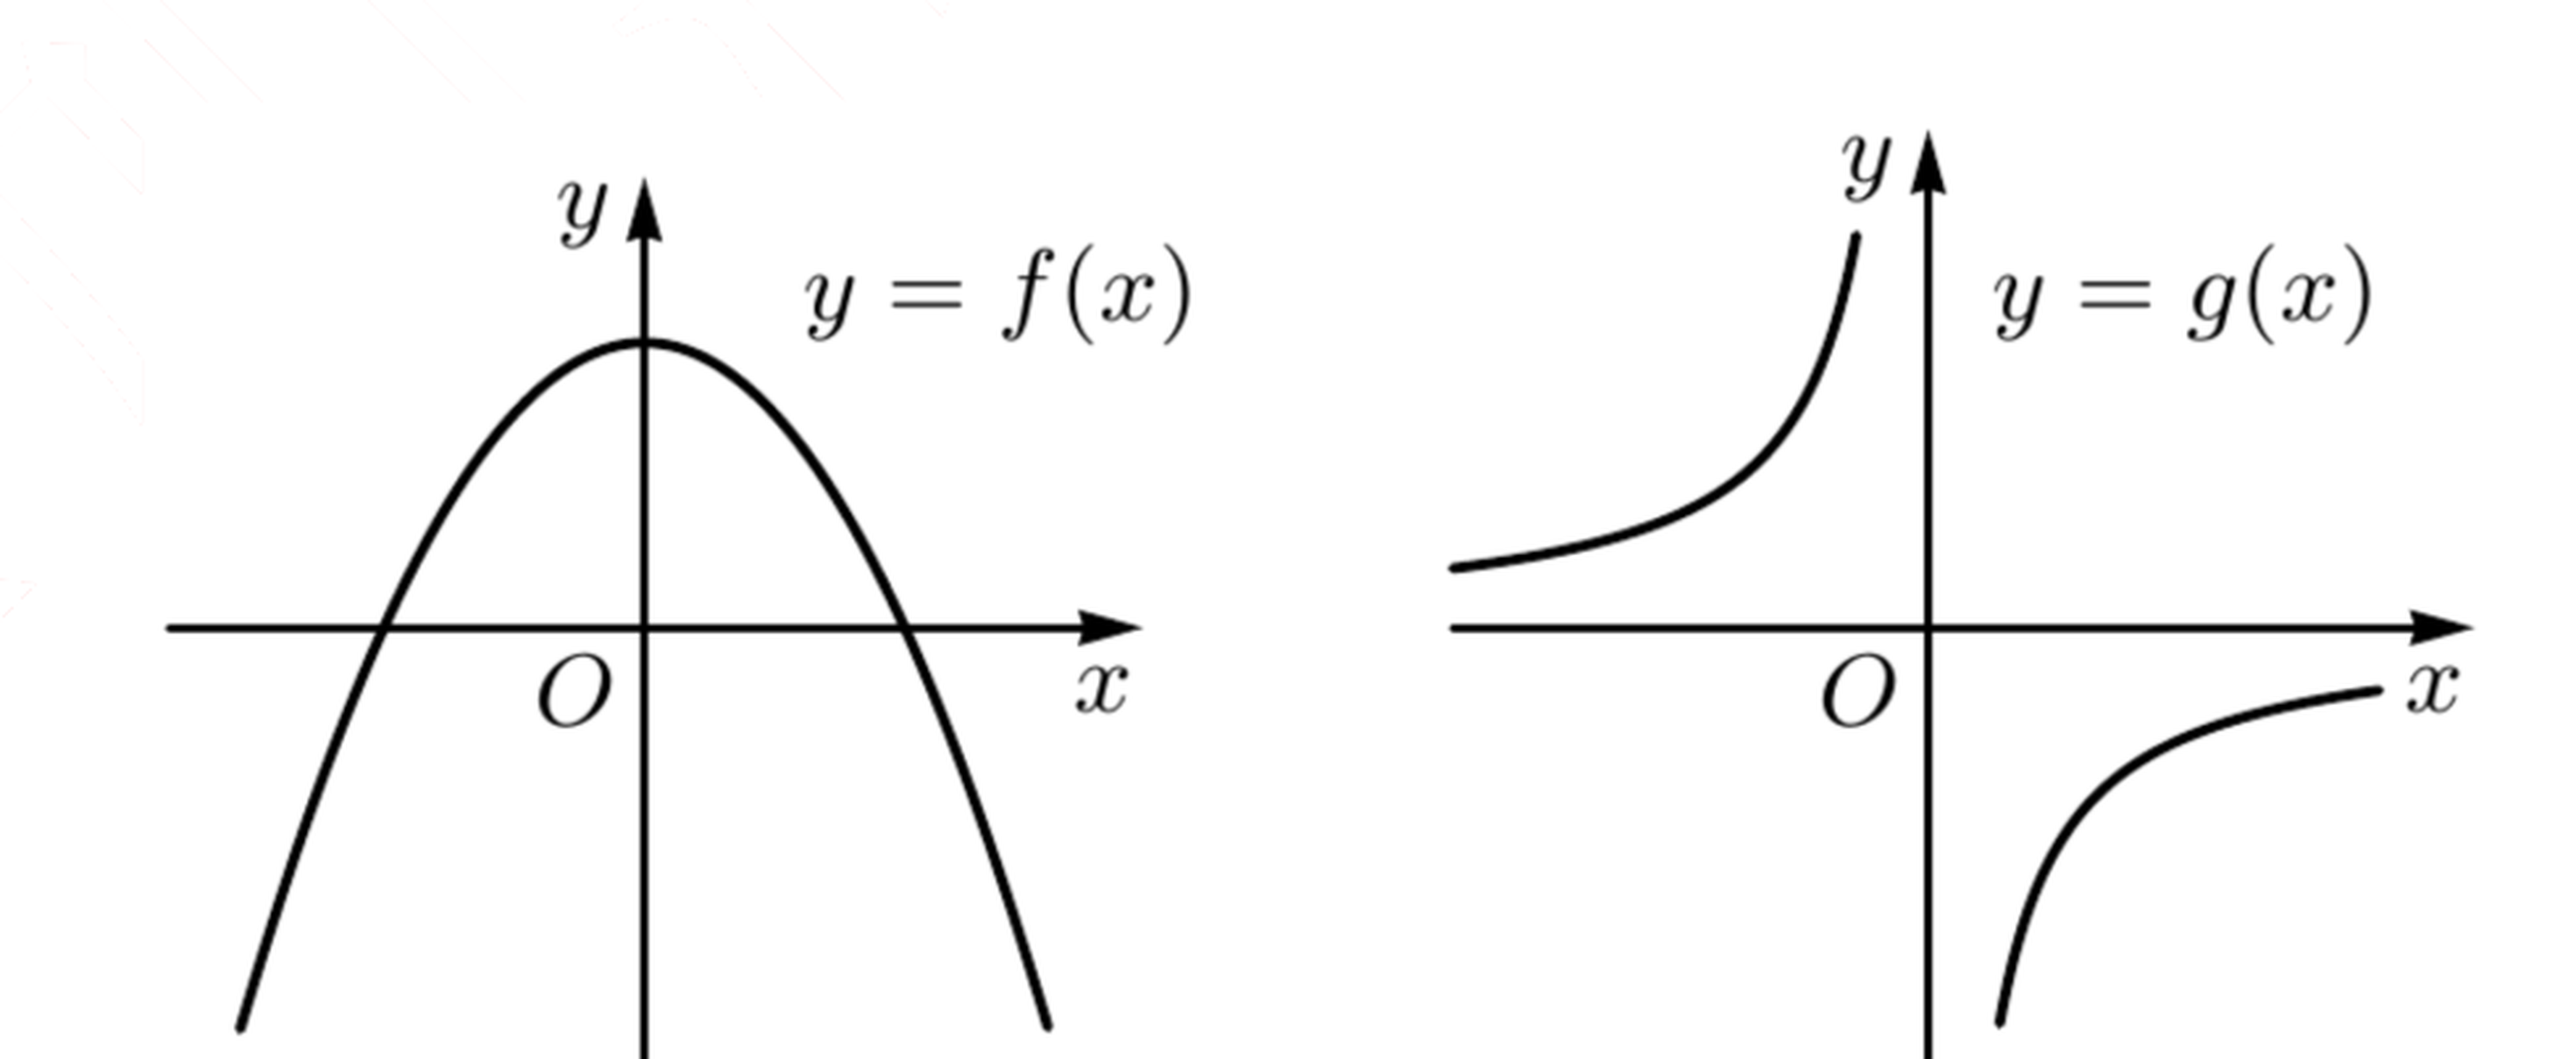
\includegraphics[width=0.72\textwidth]{figures/gao134_q13_graphs.png}\\[0.6em]
% A/B/C/D 四幅函数图象选项取原卷 04 页截图去粉色水印，按原卷一行四幅排布合并为一张
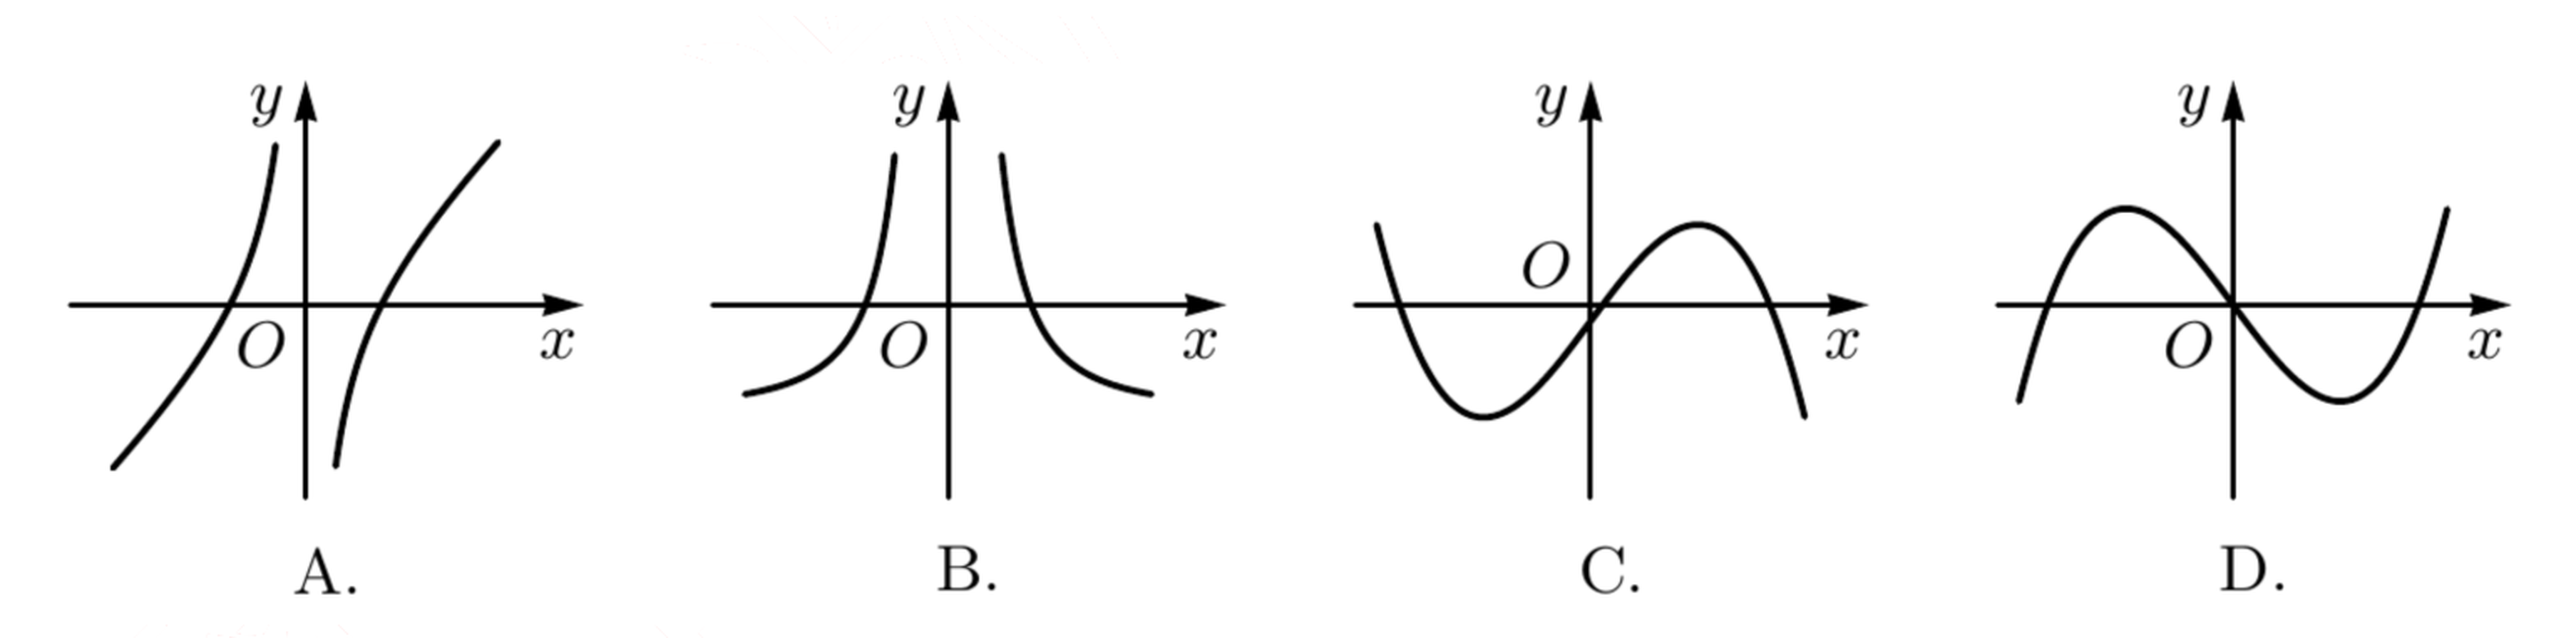
\includegraphics[width=0.90\textwidth]{figures/gao134_q13_options.png}
\end{center}

\ifanswer
\solbegin
\step{$f(x)$ 为偶函数，$g(x)$ 为奇函数，因此 $f(x)g(x)$ 为奇函数，排除 B.}
\step{又 $x=0$ 不在乘积函数的定义域内，其图象在 $y$ 轴上没有点，排除 C、D，}
\step{故选 $A$.}
\solend
\fi

\item 设全集为自然数集 $\N$，$E=\{x\mid x=2n,n\in\N\}$，$F=\{x\mid x=4n,n\in\N\}$，那么集合 $\N$ 可以表示成\mbox{（\quad）}

\keepwithprev
A. $E\cap F$\qquad\qquad B. $\overline{E}\cup F$\qquad\qquad C. $\overline{F}\cup E$\qquad\qquad D. $\overline{E}\cap\overline{F}$

\ifanswer
\solbegin
\step{$F\subseteq E$，所以 $\overline{F}\cup E=\N$，故选 $C$.}
\solend
\fi

\item 已知函数 $y=f(x)$，其中 $f(x)=x^2+bx$，则“$b<0$”是“$f(f(x))$ 的最小值与 $f(x)$ 的最小值相等”的\mbox{（\quad）}

\keepwithprev
A. 充分非必要条件\qquad\qquad B. 必要非充分条件

C. 充分必要条件\qquad\qquad D. 既非充分又非必要条件

\ifanswer
\solbegin
\step{$f(x)=\left(x+\dfrac b2\right)^2-\dfrac{b^2}4$，最小值为 $-\dfrac{b^2}4$，值域为 $\left[-\dfrac{b^2}4,+\infty\right)$.}
\step{当 $b<0$ 时，$-\dfrac b2>0\geqslant-\dfrac{b^2}4$，存在 $x$ 使 $f(x)=-\dfrac b2$，}
\step{从而 $f(f(x))$ 的最小值也为 $-\dfrac{b^2}4$，充分性成立.}
\step{当 $b=0$ 时，$f(x)=x^2$，$f(f(x))=x^4$，两者最小值均为 $0$，必要性不成立.}
\step{故选 $A$.}
\solend
\fi

\item 已知 $a,b,c\in\R$，若存在常数 $M>0$，使得 $a^2+b^2+c^2<M$，则称 $(a,b,c)$ 是有界数组. 对以下两个命题：

①若 $\lvert a^2+b+c\rvert+\lvert a^2+b-c\rvert\leqslant1$，则 $(a,b,c)$ 是有界数组；

②若 $\lvert a^2+b+c\rvert+\lvert a+b^2-c\rvert\leqslant1$，则 $(a,b,c)$ 是有界数组.% ②第二项为 \lvert a+b^2-c\rvert，与①刻意不同，照录

下列判断正确的是\mbox{（\quad）}

\keepwithprev
A. ①和②均为真命题\qquad\qquad B. ①和②均为假命题

C. ①为真命题，②为假命题\qquad D. ①为假命题，②为真命题

\ifanswer
\solbegin
\step{①取 $a=t,b=-t^2,c=0$，条件左端为 $0$，而 $a^2+b^2+c^2=t^2+t^4$ 可任意大，}
\step{故①为假命题.}
\step{②由条件，$a^2+a+b^2+b\leqslant\lvert a^2+b+c\rvert+\lvert a+b^2-c\rvert\leqslant1$.}
\step{由 $(a+1)^2+(b+1)^2\geqslant0$，得 $a^2+b^2\leqslant2(a^2+a+b^2+b)+2\leqslant4$.}
\step{又 $\lvert c\rvert\leqslant\lvert a^2+b+c\rvert+a^2+\lvert b\rvert\leqslant1+4+2=7$，故 $a^2+b^2+c^2\leqslant53<54$，}
\step{可取 $M=54$，故②为真命题.}
\step{故选 $D$.}
\solend
\fi

\end{enumerate}

\bigsec{三、解答题}

\begin{enumerate}
\setcounter{enumi}{16}

\item 已知不等式 $x^2-ax-b<0$ 的解集为 $A$，不等式 $\dfrac{3-2x}{x-1}<0$ 的解集为 $B$.

(1) 若 $a=5$，$b=-6$，求 $A\cap\overline{B}$；

(2) 若 $b=2a^2$，且 $A\cup B=B$，求实数 $a$ 的取值范围.

\ifanswer
\solbegin
\step{(1) 不等式 $\dfrac{3-2x}{x-1}<0$ 等价于 $x<1$ 或 $x>\dfrac32$，}
\step{所以 $B=(-\infty,1)\cup\left(\dfrac32,+\infty\right)$，$\overline{B}=\left[1,\dfrac32\right]$，}
\step{由 $x^2-5x+6=(x-2)(x-3)<0$，得 $A=(2,3)$，因此 $A\cap\overline{B}=\varnothing$.}
\step{(2) $A\cup B=B\Leftrightarrow A\subseteq B$，且 $x^2-ax-2a^2=(x-2a)(x+a)$，}
\step{当 $a=0$ 时，$A=\varnothing$，满足条件.}
\step{当 $a>0$ 时，$A=(-a,2a)$，$-a<0<1$，$A\subseteq B\Leftrightarrow2a\leqslant1$，得 $0<a\leqslant\dfrac12$.}
\step{当 $a<0$ 时，$A=(2a,-a)$，$2a<0<1$，$A\subseteq B\Leftrightarrow-a\leqslant1$，}
\step{得 $-1\leqslant a<0$.}
\step{因此 $a$ 的取值范围为 $\left[-1,\dfrac12\right]$.}
\solend
\fi

\item 为了在夏季降温和冬季供暖时减少能源损耗，房屋的屋顶和外墙需要建造隔热层. 某幢建筑物要建造可使用 $30$ 年的隔热层，每厘米厚的隔热层建造成本为 $9$ 万元. 该建筑物每年的能源消耗费用 $C$（万元）与隔热层厚度 $x$（cm）满足如下关系式：$C=\dfrac{k}{3x+5}$（$0\leqslant x\leqslant10$）. 若不建隔热层，每年能源消耗费用为 $8$ 万元. 设 $y$（万元）为隔热层建造费用与 $30$ 年的能源消耗费用之和.

(1) 求 $k$ 的值及 $y$ 的表达式；

(2) 隔热层修建多厚时，总费用 $y$ 最小？并求最小值.

\ifanswer
\solbegin
\step{(1) 不建隔热层时 $x=0$，$C=8$，所以 $\dfrac k5=8$，得 $k=40$.}
\step{隔热层建造费用为 $9x$ 万元，$30$ 年的能源消耗费用为 $30\times\dfrac{40}{3x+5}$ 万元.}
\step{因此 $y=9x+\dfrac{1200}{3x+5}$，$0\leqslant x\leqslant10$.}
\step{(2) 令 $t=3x+5$，则 $5\leqslant t\leqslant35$，且 $y=3t+\dfrac{1200}{t}-15$，}
\step{因为 $t>0$，由基本不等式得 $y\geqslant2\sqrt{3t\cdot\dfrac{1200}{t}}-15=105$，}
\step{当且仅当 $3t=\dfrac{1200}{t}$，即 $t=20$时取等号，此时 $x=5\in[0,10]$，}% 原卷"20"与"时"之间未留空，照录
\step{所以隔热层厚度为 $5$ cm 时，总费用最小，最小值为 $105$ 万元.}
\solend
\fi

\item 已知 $f(x)=ax^2+\dfrac1x$，其中 $a$ 为常数.

(1) 若 $a\in(1,3)$，判断函数 $y=f(x)$ 在 $[1,2]$ 上的单调性，并用定义证明；

(2) 求函数 $y=f(x)-x-\dfrac1x$ 在 $[1,2]$ 上的最大值 $g(a)$.

\ifanswer
\solbegin
\step{(1) 任取 $x_1,x_2\in[1,2]$，且 $x_1<x_2$，}
\step{则 $f(x_2)-f(x_1)=(x_2-x_1)\left[a(x_1+x_2)-\dfrac1{x_1x_2}\right]$，}
\step{由 $a>1$，$x_1+x_2\geqslant2$，$x_1x_2\geqslant1$，得 $a(x_1+x_2)-\dfrac1{x_1x_2}>2-1>0$，}
\step{因此 $f(x_2)>f(x_1)$，$f(x)$ 在 $[1,2]$ 上为严格增函数.}
\step{(2) 令 $h(x)=f(x)-x-\dfrac1x=ax^2-x$，其中 $x\in[1,2]$.}
\step{若 $a=0$，则 $h(x)=-x$，所以 $h(x)_{max}=h(1)=-1$；}
\step{若 $a<0$，二次函数的图象的对称轴为 $x=\dfrac1{2a}<0$，}
\step{所以 $y=h(x)$ 在 $[1,2]$ 上是严格减函数，所以 $h(x)_{max}=h(1)=a-1$；}
\step{若 $a>0$ 且 $\dfrac1{2a}>\dfrac32$，即 $0<a<\dfrac13$ 时，$h(x)_{max}=h(1)=a-1$.}
\step{若 $a>0$ 且 $\dfrac1{2a}\leqslant\dfrac32$，即 $a\geqslant\dfrac13$ 时，$h(x)_{max}=h(2)=4a-2$.}
\step{综上所述，$g(a)=\begin{cases}a-1,a<\dfrac13\\4a-2,a\geqslant\dfrac13\end{cases}$.}
\solend
\fi

\item 已知 $f(x)=\dfrac{ax^2+1}{bx+c}$（$a,b,c\in\Z$）.

(1) 若函数 $y=f(x)$ 是奇函数，且 $f(1)=2$，$f(2)<3$，求 $a,b,c$ 的值；

(2) 若函数 $y=f(x)$ 是偶函数，且 $ac<0$，$f(2a^2+a+1)<f(-3a^2+2a-1)$，求 $a$ 的值；

(3) 若 $b=a+c^2$，且满足不等式 $\lvert f(x)\rvert\geqslant1$ 的 $x$ 的最大值为 $0$，求 $c$ 的值.

\ifanswer
\solbegin
\step{(1) 由 $f(-x)=-f(x)$，交叉相乘得 $2c(ax^2+1)=0$ 恒成立，}
\step{因此 $c=0$，$b\neq0$.}
\step{由 $f(1)=2$，得 $a+1=2b$，}
\step{于是 $f(2)=\dfrac{4a+1}{2b}=4-\dfrac3{2b}<3\Leftrightarrow0<b<\dfrac32$，}
\step{因为 $b\in\Z$，所以 $b=1$，进而 $a=1$，$c=0$.}
\step{(2) 由 $f(-x)=f(x)$，交叉相乘得 $2bx(ax^2+1)=0$ 恒成立，因此 $b=0$.}
\step{此时 $f(x)=\dfrac ac x^2+\dfrac1c$，且 $\dfrac ac<0$.}
\step{设 $u=2a^2+a+1$，$v=-3a^2+2a-1$.}
\step{方程 $2a^2+a+1=0$ 与 $3a^2-2a+1=0$ 的判别式分别为 $-7$ 与 $-8$，}
\step{都小于 $0$，所以 $u>0$，$v<0$.}
\step{于是 $f(u)<f(v)\Leftrightarrow u^2>v^2\Leftrightarrow u>-v\Leftrightarrow-a^2+3a>0\Leftrightarrow0<a<3$，}
\step{因为 $a\in\Z$，所以 $a=1$ 或 $a=2$.}
\step{(3) 因为解集的最大值为 $0$，所以 $f(0)$ 有定义且 $\lvert f(0)\rvert\geqslant1$，}
\step{即 $c\neq0$，$\left\lvert\dfrac1c\right\rvert\geqslant1$，结合 $c\in\Z$，得 $c=\pm1$，从而 $b=a+1$.}
\step{当 $x=2$ 时，分母 $2a+2+c$ 为奇数，必不为 $0$；}
\step{又因为 $2>0$，必须有 $\lvert f(2)\rvert<1\Leftrightarrow\lvert4a+1\rvert<\lvert2a+2+c\rvert$，}
\step{若 $c=-1$，则 $(4a+1)^2<(2a+1)^2\Leftrightarrow4a(3a+1)<0\Leftrightarrow-\dfrac13<a<0$，}
\step{不存在满足条件的整数 $a$.}
\step{若 $c=1$，则 $(4a+1)^2<(2a+3)^2\Leftrightarrow4(3a+2)(a-1)<0\Leftrightarrow-\dfrac23<a<1$，}
\step{所以 $a=0$，$b=1$，此时 $f(x)=\dfrac1{x+1}$，}
\step{且 $\lvert f(x)\rvert\geqslant1\Leftrightarrow0<\lvert x+1\rvert\leqslant1\Leftrightarrow x\in[-2,-1)\cup(-1,0]$，}
\step{解集的最大值确为 $0$，因此 $c=1$.}
\solend
\fi

\item 已知函数 $y=f(x)$ 的定义域为 $\R$，且当 $x>0$ 时，$f(x)=\dfrac1{x+1}$. 对任意 $x_0\in\R$，定义集合 $D(x_0)=\{d\mid f(x_0+d)>f(x_0)\}$.

(1) 若当 $x\leqslant0$ 时，$f(x)=-2x+1$，求函数 $y=f(x)$ 的值域；

(2) 若 $y=f(x)$ 是偶函数，且 $f(0)=1$，求证：$D(-2)=\{-d\mid d\in D(2)\}$；

(3) 若 $y=f(x)$ 是奇函数，且 $x_1x_2\neq0$，求证：“$f(x_1)\leqslant f(x_2)$”的充要条件是\!\mbox{“$D(x_2)\subseteq D(x_1)$”}.

\ifanswer
\solbegin
\step{(1) 当 $x>0$ 时，$0<f(x)<1$；当 $x\leqslant0$ 时，$f(x)=-2x+1\geqslant1$.}
\step{函数的值域为 $(0,1)\cup[1,+\infty)=(0,+\infty)$.}
\step{(2) 由 $f(x)$ 是偶函数及 $f(0)=1$，得 $f(x)=\dfrac1{1+\lvert x\rvert}$，且 $f(2)=f(-2)=\dfrac13$.}
\stepm{法一：}{$D(2)=\left\{d\mid\dfrac1{1+\lvert2+d\rvert}>\dfrac13\right\}=\{d\mid\lvert2+d\rvert<2\}=(-4,0)$，}
\step{$D(-2)=\left\{d\mid\dfrac1{1+\lvert-2+d\rvert}>\dfrac13\right\}=\{d\mid\lvert-2+d\rvert<2\}=(0,4)$，}
\step{因此 $\{-d\mid d\in D(2)\}=(0,4)=D(-2)$.}
\stepm{法二：}{任取 $d\in D(-2)$，由定义得 $f(-2+d)>f(-2)$.}
\step{因为 $y=f(x)$ 是偶函数，所以对任意的实数 $x$，有 $f(-x)=f(x)$，}
\step{因此 $f(-2+d)=f(-(-2+d))=f(2-d)$，且 $f(-2)=f(2)$.}
\step{所以不等式 $f(-2+d)>f(-2)$ 等价于 $f(2-d)>f(2)$，}
\step{这恰好是 $-d\in D(2)$ 的定义，}
\step{所以 $d\in D(-2)\Leftrightarrow-d\in D(2)$，故 $D(-2)=\{-d\mid d\in D(2)\}$.}
\step{(3) 由 $f(x)$ 是奇函数，得 $f(0)=0$；}
\step{当 $x<0$ 时，$f(x)=-f(-x)=-\dfrac1{1-x}=\dfrac1{x-1}$；}
\step{所以 $f(x)=\begin{cases}\dfrac1{x-1},&x<0\\0,&x=0;\\\dfrac1{x+1},&x>0\end{cases}$}
% 2026-11-15 回原图订正：原卷 11 页此 cases 块末无句点，本稿初转顺手补了西文句点，今删去（Q19 08 页同类块末有句点，照录保留）。
\step{当 $x_0<0$ 时，$D(x_0)=\{d\mid f(x_0+d)>f(x_0)\}=(-\infty,0)\cup[-x_0,+\infty)$，}
\step{当 $x_0=0$ 时，$D(0)=\{d\mid f(0+d)>f(0)\}=(0,+\infty)$，}
\step{当 $x_0>0$ 时，$D(x_0)=\{d\mid f(x_0+d)>f(x_0)\}=(-x_0,0)$.}
\stepm{先证明必要性.}{若 $f(x_1)\leqslant f(x_2)$，仅需讨论三类情形：}
\step{若 $x_2\leqslant x_1<0$，}
\step{则 $D(x_1)=(-\infty,0)\cup[-x_1,+\infty),D(x_2)=(-\infty,0)\cup[-x_2,+\infty)$，}
\step{故 $D(x_2)\subseteq D(x_1)$；}
\step{若 $0<x_2\leqslant x_1$，则 $D(x_1)=(-x_1,0),D(x_2)=(-x_2,0)$，}
\step{故 $D(x_2)\subseteq D(x_1)$；}
\step{若 $x_1<0<x_2$，则 $D(x_1)=(-\infty,0)\cup[-x_1,+\infty),D(x_2)=(-x_2,0)$，}
\step{故 $D(x_2)\subseteq D(x_1)$.}
\stepm{再证明充分性.}{若 $D(x_2)\subseteq D(x_1)$，}
\step{若 $x_1<0,x_2<0$，}
\step{则 $D(x_1)=(-\infty,0)\cup[-x_1,+\infty),D(x_2)=(-\infty,0)\cup[-x_2,+\infty)$，}
\step{由 $D(x_2)\subseteq D(x_1)$ 得 $x_2\leqslant x_1$，}
\step{又 $y=f(x)$ 在 $(-\infty,0)$ 上是严格减函数，所以 $f(x_1)\leqslant f(x_2)$；}
\step{若 $x_1>0,x_2>0$，则 $D(x_1)=(-x_1,0),D(x_2)=(-x_2,0)$，}
\step{由 $D(x_2)\subseteq D(x_1)$ 得 $x_2\leqslant x_1$，}
\step{又 $y=f(x)$ 在 $(0,+\infty)$ 上是严格减函数，所以 $f(x_1)\leqslant f(x_2)$；}
\step{若 $x_1<0,x_2>0$，则 $f(x_1)<0<f(x_2)$，结论成立；}
\step{若 $x_1>0,x_2<0$，此时 $D(x_1)=(-x_1,0)$ 中只有负数，}
\step{而 $D(x_2)=(-\infty,0)\cup[-x_2,+\infty)$ 中有正数，$D(x_2)\subseteq D(x_1)$ 不成立.}
\step{综上，“$f(x_1)\leqslant f(x_2)$”的充要条件是“$D(x_2)\subseteq D(x_1)$”.}
\solend
\fi

\end{enumerate}

\end{document}
"
%
% ① 原始材料：微信公众号"魔都数学加油站"文章，作者破晓，2026-11-15 18:04 发布；
% 连载"27学年高一134"，原文标题"27学年高一134——2026-2027年上海市华师大二附中高一上期中"；
% 原文链接：https://mp.weixin.qq.com/s/bQlkmlGdCtAlytY331vf3g。
% 正文为 13 张 PNG 页（01、04、06、08、09、10、11、12、13 为 2560x3620；
% 02、03、05、07 为 4762x6735，同一篇各页分辨率不同，逐页按各自分辨率裁图核对），
% 题目下印有【解析】，为讲评版。题目、解析均据原图转录；卷面粉红色水印
% "魔都数学加油站"及公众号页脚未录入。
% 全卷 2 幅插图，均在第 04 页：第 13 题题干 y=f(x)、y=g(x) 两幅函数图象合并裁为
% figures/gao134_q13_graphs.png，第 13 题 A/B/C/D 四幅函数图象选项合并裁为
% figures/gao134_q13_options.png；两图均取原卷 04 页截图 3× LANCZOS 放大、
% 白化粉色水印（只白化浅粉色 R>175 且 G>140 且 B>140 的像素，保留红色标签）。
% 注意：本卷 Q13 四幅选项在原卷排为"一行四幅"（1×4），并非 高一132 第 14 题
% 的 2×2 排布，本稿按原卷 1×4 合并裁为一张，不重排、不用 TikZ 重绘。
%
% 卷首标题：原卷印作"2026-2027 年华师大二附中高一上期中"（公众号标题中的"上海市"
% 卷面标题行没有，本稿照卷面），年份区间按全稿惯例排 en dash；原卷未印副标题，
% 本卷为期中卷、跨集合与常用逻辑用语／不等式／函数三章，按题目内容标为
% "集合与常用逻辑用语、不等式、函数"（与 125／126／128／129／131／132／133 同期中卷口径相同）：
% 集合与逻辑见 Q6、Q10、Q14、Q16、Q17、Q21，不等式见 Q3、Q7、Q9、Q11、Q15、Q18、Q19，
% 函数（函数性质、二分法、奇偶性、基本不等式应用）见 Q4、Q5、Q8、Q12、Q13、Q20。
%
% 题号体例：本卷共 19 题——一、填空题 3—12（10 题）、二、选择题 13—16（4 题）、
% 三、解答题 17—21（5 题）。三节分别 \setcounter{enumi}{2}／{12}／{16}。
% 第 13 页仅为 Q21 (3) 解析续尾，全卷无「四、附加题」。
%
% ② 与原卷的排版差异：
%   ① 原文从第 3 题起，本稿保留原题号（见上"题号体例"）；
%   ② 原卷每题下直接印【解析】，本稿按全稿惯例置于答案版；第 13—16 题答案均在
%      解析末句"故选 …"，题干括号内留空、不另提 \ans{}（四题均无独立答案段）；
%      全卷无只印括号内答案、无解析的选择题；
%   ③ 原卷未印副标题，本稿按"知识模块"口径补出；
%   ④ 原卷填空横线按全稿惯例排为 \blankline[4.4em]；选择题括号排 \mbox{（\quad）}、
%      每个选项段前按惯例加 \keepwithprev（Q13 四选项为图，守卫前行为 \begin{center}；
%      Q15、Q16 四选项分两行排，\keepwithprev 只加在 A. 行前）；解答题不留作答区、
%      不加 \anspace（原卷为讲评版，与 129／131／132／133 同）；
%   ⑤ 原卷数集印黑板粗体（Q7／Q11／Q12／Q16／Q21 的 R、Q14／Q20 的 N、Q20 的 Z），
%      按全稿惯例统一排 \R／\N／\Z；绝对值排 \lvert…\rvert，集合描述竖线排 \mid；不等号按全稿惯例排
%      \leqslant／\geqslant；补集照原卷上划线排 \overline{B}、\overline{E}、\overline{F}；
%   ⑥ 子题标号 (1)(2)(3) 与括注原卷均用半角括号，照录（与 131／132／133 同）；
%      圈数字 ①② 照录；原卷 Q21 (2) 解析"法一：""法二："与 Q21 (3) 解析
%      "先证明必要性.""再证明充分性."四处标签印红色加粗，按 高一53／108／133 成例排
%      \stepm{法一：}／\stepm{法二：}／\stepm{先证明必要性.}／\stepm{再证明充分性.}
%      （加粗着色、不引入红色，不动 common.sty）；Q8 解析"第 1 步：""第 2 步：""
%      "第 3 步："原卷印黑色常规宋体（非红非粗），照录为普通 \step 行内文字；
%   ⑦ 数学式内半角逗号照录（如 Q6 $A=\{0,1,2,3\}$、Q14 $x=2n,n\in\N$、
%      Q16 $a,b,c\in\R$ 与 $a=t,b=-t^2,c=0$、Q19 $x_1,x_2\in[1,2]$、
%      Q20 $a,b,c\in\Z$、Q21 $x_1<0,x_2<0$ 与 $D(x_1)=(-x_1,0),D(x_2)=(-x_2,0)$）；
%      原卷行末全角句点按全稿惯例从宽排西文句点；cases 块末的句点逐处照录：
%      Q19 解析（08 页）块末原卷有句点照录、Q21 (3) 解析（11 页）块末原卷无句点不补，
%      两处原卷自身不统一（2026-11-15 回原图核对，本稿初转曾顺手补句点，已删去）；
%   ⑧ 原卷 Q8 解析跨 01—02 页、Q10 解析跨 02—03 页、Q12 解析跨 03—04 页、
%      Q16 解析跨 05—06 页、Q17 解析跨 06—07 页、Q20 解析跨 08—10 页、
%      Q21 解析跨 10—13 页，本稿按题合并连续排版；末页第 13 页为
%      Q21 (3) 解析续尾与"综上"一句，按实际印刷行单列；
%   ⑨ 题干中的中文弯引号按原卷照录（Q10 研究问题、Q15 条件、Q21 (3) 充要条件），
%      注释内一律 ASCII 引号。
%
% 判别式字形：全卷仅 Q9 解析末行出现一处判别式记号
%   "两值均满足 $\Delta=p^2-4p=18\mp12\sqrt2>0$"，逐处放大核对，原卷印高三角
%   $\Delta$（等腰、高，实测高宽比约 1.14），照录 \Delta；卷内无扁三角 \triangle，
%   与 高一132 同题排 $\triangle$、高一133 部分判别式排 $\triangle$ 均不同。
%
% 子集符号：Q6 题干 $C\subseteq A$、$C\subseteq B$ 与解析 $C\subseteq A\cap B$、
%   Q14 解析 $F\subseteq E$、Q17 解析 $A\subseteq B$、Q21 题干与解析各处的
%   $D(x_2)\subseteq D(x_1)$，全部印带下划线的 $\subseteq$，逐处放大核对，
%   照录 \subseteq；全卷未出现单线 \subset。
%
% 原卷存疑照录（均照录未改，正文对应处另有 % 注）：
%   第 6 题题干集合 $A=\{0,1,2,3\}$ 三个逗号后不留空，紧邻的 $B=\{0,2,4,5\}$
%      三个逗号后却留空，同卷同一行两集合排字不一，照录其逗号均为半角；
%   第 16 题命题②作 $\lvert a^2+b+c\rvert+\lvert a+b^2-c\rvert\leqslant1$，
%      与命题①第二项 $\lvert a^2+b-c\rvert$ 不同（①无 $b$ 的平方、②有），
%      两命题刻意不同，照录；解析"②由条件，$a^2+a+b^2+b\leqslant\cdots$"
%      由两项相加直接得到，照录；
%   第 18 题 (2) 解析"即 $t=20$时取等号"中"20"与"时"之间原卷未留空，照录；
%   第 19 题解析 $h(x)_{max}$ 的"max"下标三处字形不一（斜体／正体混排），照录；
%   第 20 题 (1)(2) 解析"由 $f(-x)=-f(x)$，交叉相乘得……"与"由 $f(-x)=f(x)$，
%      交叉相乘得……"两处措辞照录；
%   第 21 题 (2) 原卷并存"法一"（集合计算）与"法二"（定义推证）两套证明，照录不删。
%
% 行数复核：逐题数 \step/\stepm 条数，合计 134 条（Q3：2；Q4：1；Q5：1；Q6：1；
% Q7：2；Q8：4；Q9：3；Q10：4；Q11：5；Q12：8；Q13：3；Q14：1；Q15：5；
% Q16：7；Q17：9；Q18：7；Q19：11；Q20：22；Q21：38），与原卷印刷行逐题相等
% （cases 块作一个印刷行计）。第 13—16 题答案在解析末句，括号内留空、不另提 \ans{}；
% 第 21 题四条 \stepm 计入 38 条内。
%
\documentclass[a4paper,11pt]{article}
\usepackage{common}

\begin{document}

\examtitlest[3]{2026--2027 年华师大二附中高一上期中}{集合与常用逻辑用语、不等式、函数}

\bigsec{一、填空题}

\begin{enumerate}
\setcounter{enumi}{2}

\item 不等式 $\lvert 2x+1\rvert\geqslant3$ 的解集为\blankline[4.4em].

\ifanswer
\solbegin
\step{$\lvert 2x+1\rvert\geqslant3\Leftrightarrow 2x+1\leqslant-3$ 或 $2x+1\geqslant3\Leftrightarrow x\leqslant-2$ 或 $x\geqslant1$，}
\step{故解集为 $(-\infty,-2]\cup[1,+\infty)$.}
\solend
\fi

\item 函数 $y=\sqrt{x+1}+\dfrac1x$ 的定义域为\blankline[4.4em].

\ifanswer
\solbegin
\step{$x+1\geqslant0$ 且 $x\neq0$，得定义域为 $[-1,0)\cup(0,+\infty)$.}
\solend
\fi

\item 已知等式 $3x^2-4x-2=a(x-1)^2+b(x-1)+c$ 恒成立，其中 $a$、$b$、$c$ 为常数，则 $a-b+c=$\blankline[4.4em].

\ifanswer
\solbegin
\step{令 $x=0$，得 $a-b+c=-2$.}
\solend
\fi

\item 已知集合 $A=\{0,1,2,3\}$，$B=\{0,2,4,5\}$，$C\subseteq A$，$C\subseteq B$，符合条件的集合 $C$ 有\blankline[4.4em]个.% 原卷 A 的逗号后不留空、B 的逗号后留空，排字不一，照录

\ifanswer
\solbegin
\step{$C\subseteq A\cap B=\{0,2\}$，所以符合条件的集合 $C$ 有 $2^2=4$ 个.}
\solend
\fi

\item 设 $a$、$b\in\R$，且 $a^2+4b^2=2$，则 $ab$ 的最大值为\blankline[4.4em].

\ifanswer
\solbegin
\step{$(a-2b)^2=a^2+4b^2-4ab=2-4ab\geqslant0$，得 $ab\leqslant\dfrac12$，}
\step{当且仅当 $a=2b=\pm1$ 时取等号，故 $ab$ 的最大值为 $\dfrac12$.}
\solend
\fi

\item 已知函数 $y=x(13-2x)^2-140$，用二分法求函数在区间 $(3,4)$ 上的零点时，第 3 步应计算 $x=$\blankline[4.4em]的函数值.

\ifanswer
\solbegin
\step{记 $f(x)=x(13-2x)^2-140$，则 $f(3)=7>0$，$f(4)=-40<0$.}
\step{第 1 步：$f\left(\dfrac72\right)=-14<0$，区间缩小为 $\left(3,\dfrac72\right)$.}
\step{第 2 步：$f\left(\dfrac{13}4\right)=-\dfrac{43}{16}<0$，区间缩小为 $\left(3,\dfrac{13}4\right)$.}
\step{第 3 步：应计算 $x=\dfrac{3+\frac{13}4}2=\dfrac{25}8$ 的函数值.}
\solend
\fi

\item 已知一元二次方程 $x^2+px+p=0$ 的两个实根分别为 $x_1$、$x_2$，且 $x_1^2x_2+x_2^2x_1=-18$，则 $p=$\blankline[4.4em].% 判别式 \Delta 高三角，逐处放大核对

\ifanswer
\solbegin
\step{由韦达定理，$x_1+x_2=-p$，$x_1x_2=p$，}
\step{则 $x_1^2x_2+x_2^2x_1=x_1x_2(x_1+x_2)=-p^2=-18\Rightarrow p=\pm3\sqrt2$，}
\step{两值均满足 $\Delta=p^2-4p=18\mp12\sqrt2>0$，故 $p=\pm3\sqrt2$.}
\solend
\fi

\item 研究问题：“已知关于 $x$ 的不等式 $ax^2-bx+c>0$ 的解集为 $(1,2)$，解关于 $x$ 的不等式 $cx^2-bx+a>0$”，有如下解法：

解：由 $ax^2-bx+c>0\Rightarrow a-b\left(\dfrac1x\right)+c\left(\dfrac1x\right)^2>0$，令 $y=\dfrac1x$，则 $y\in\left(\dfrac12,1\right)$，

所以不等式 $cx^2-bx+a>0$ 的解集为 $\left(\dfrac12,1\right)$.

参考上述解法，已知关于 $x$ 的不等式 $\dfrac{k}{x+a}+\dfrac{x+b}{x+c}<0$ 的解集为 $(-3,-1)\cup(2,4)$，则关于 $x$ 的不等式 $\dfrac{kx}{ax-1}+\dfrac{bx-1}{cx-1}<0$ 的解集为\blankline[4.4em].

\ifanswer
\solbegin
\step{当 $x=0$ 时，所求不等式左端为 $1$，不满足不等式.}
\step{当 $x\neq0$ 时，两个分式的分子、分母同除以 $x$，得 $\dfrac{k}{a-\frac1x}+\dfrac{b-\frac1x}{c-\frac1x}<0$.}
\step{令 $t=-\dfrac1x$，则所求不等式化为 $\dfrac{k}{t+a}+\dfrac{t+b}{t+c}<0$，即 $-\dfrac1x\in(-3,-1)\cup(2,4)$，}
\step{解得 $x\in\left(-\dfrac12,-\dfrac14\right)\cup\left(\dfrac13,1\right)$.}
\solend
\fi

\item 已知 $a\in(0,+\infty)$，若对任意的 $x\in(0,+\infty)$，均有 $\lvert x^2-a\rvert+\lvert x+b\rvert=\lvert x^2+x-a+b\rvert$，则 $a^2-b^2$ 的最小值为\blankline[4.4em].

\ifanswer
\solbegin
\step{原等式成立的充要条件是 $(x^2-a)(x+b)\geqslant0$.}
\step{当 $0<x<\sqrt a$ 时须有 $x+b\leqslant0$；当 $x>\sqrt a$ 时须有 $x+b\geqslant0$，因此 $b=-\sqrt a$.}
\step{此时 $(x^2-a)(x+b)=(x+\sqrt a)(x-\sqrt a)^2\geqslant0$，满足题意.}
\step{$a^2-b^2=a^2-a=\left(a-\dfrac12\right)^2-\dfrac14\geqslant-\dfrac14$，}
\step{当 $a=\dfrac12$，$b=-\dfrac{\sqrt2}2$ 时取等号，最小值为 $-\dfrac14$.}
\solend
\fi

\item 已知函数 $y=f(x)$ 在 $\R$ 上是严格增函数，当 $x\neq0$ 且 $f(x)\neq0$ 时，满足 $f(x)\cdot f\left[\dfrac1{f(x)}+\dfrac1x\right]=1$，则 $f(1)=$\blankline[4.4em].

\ifanswer
\solbegin
\step{当 $xf(x)>0$ 时，记 $t=\dfrac1{f(x)}+\dfrac1x\neq0$，则 $f(t)=\dfrac1{f(x)}\neq0$.}
\step{将 $t$ 代入题设，得 $f\left(f(x)+\dfrac1t\right)=f(x)$，严格增性给出 $f(x)+\dfrac1t=x$，}
\step{化简得 $f(x)^2+xf(x)-x^2=0$，由 $\dfrac{f(x)}x>0$ 得 $f(x)=\dfrac{\sqrt5-1}2x$.}
\step{设 $a=f(0)$，若 $a>0$，则 $f(a)>f(0)=a>0$；}
\step{若 $a<0$，则 $f(a)<f(0)=a<0$.}
\step{两种情形都有 $af(a)>0$ 且 $\dfrac{f(a)}a>1$，与上式 $\dfrac{f(a)}a=\dfrac{\sqrt5-1}2<1$ 矛盾，}
\step{因此 $f(0)=0$.}
\step{于是 $f(1)>0$，代入上式得 $f(1)=\dfrac{\sqrt5-1}2$.}
\solend
\fi

\end{enumerate}

% 第 13 题是"节标题 + 题干 + 两幅图 + 四幅选项图"约 15cm 的整块，
% 守卫只放在 \bigsec 之前；若再在 \item 之前放第二枚，会在标题已印出后才触发换页，
% 把题目推走、留下孤立节标题（切页审计 B 类）。高度须覆盖整块。
\needvspace{16cm}
\bigsec{二、选择题}

\begin{enumerate}
\setcounter{enumi}{12}

\item 已知函数 $y=f(x)$ 与 $y=g(x)$ 的图象如图所示，则函数 $y=f(x)\cdot g(x)$ 的图象可能是\mbox{（\quad）}

\keepwithprev
\begin{center}
% 题干 y=f(x)、y=g(x) 两幅函数图象取原卷 04 页截图去粉色水印，按原卷左右排布合并为一张
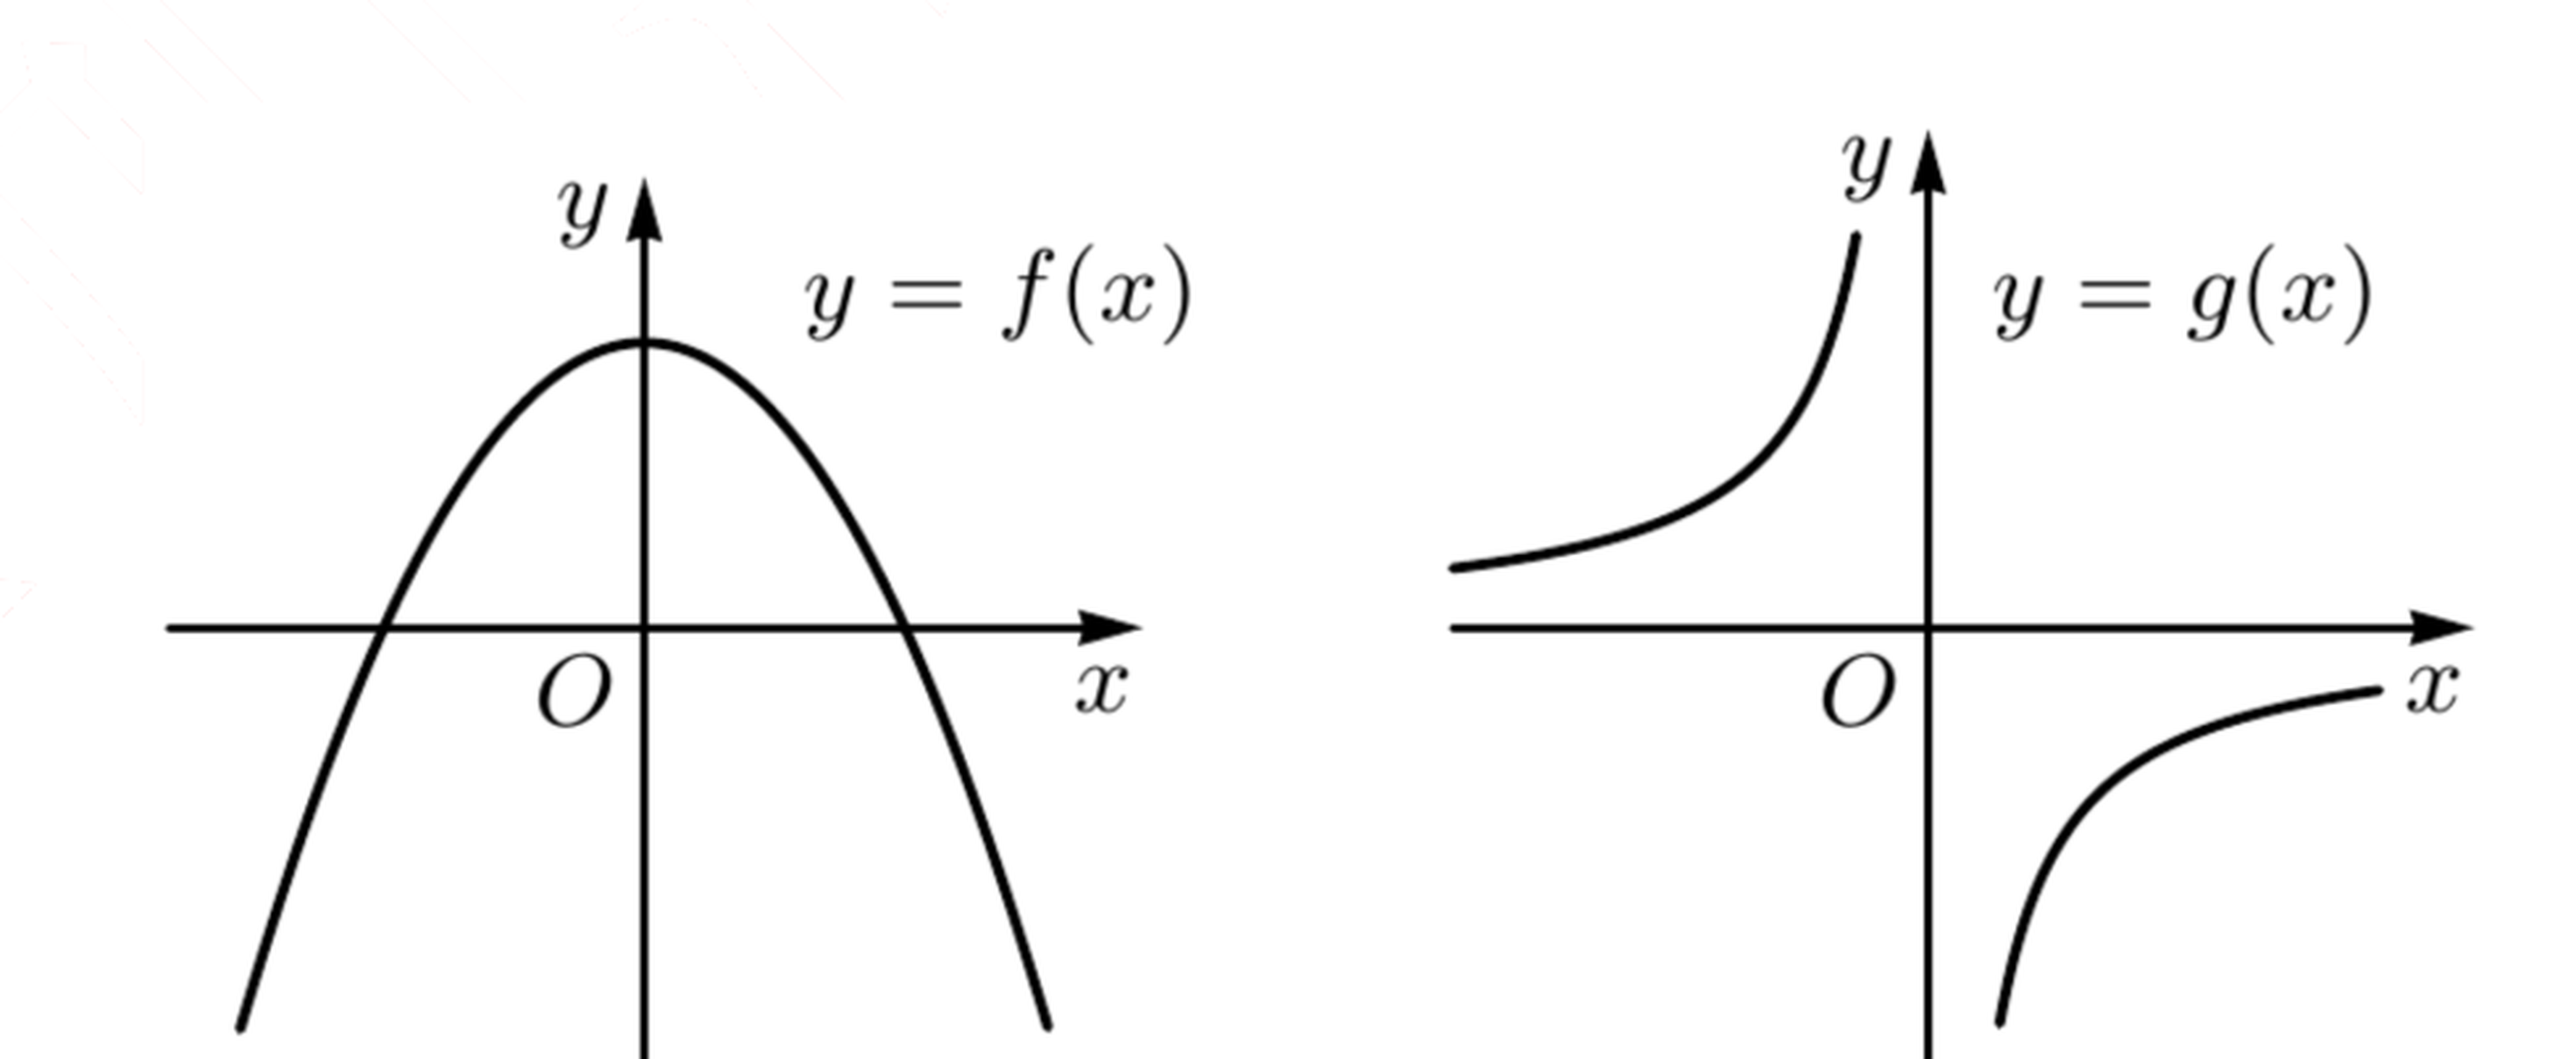
\includegraphics[width=0.72\textwidth]{figures/gao134_q13_graphs.png}\\[0.6em]
% A/B/C/D 四幅函数图象选项取原卷 04 页截图去粉色水印，按原卷一行四幅排布合并为一张
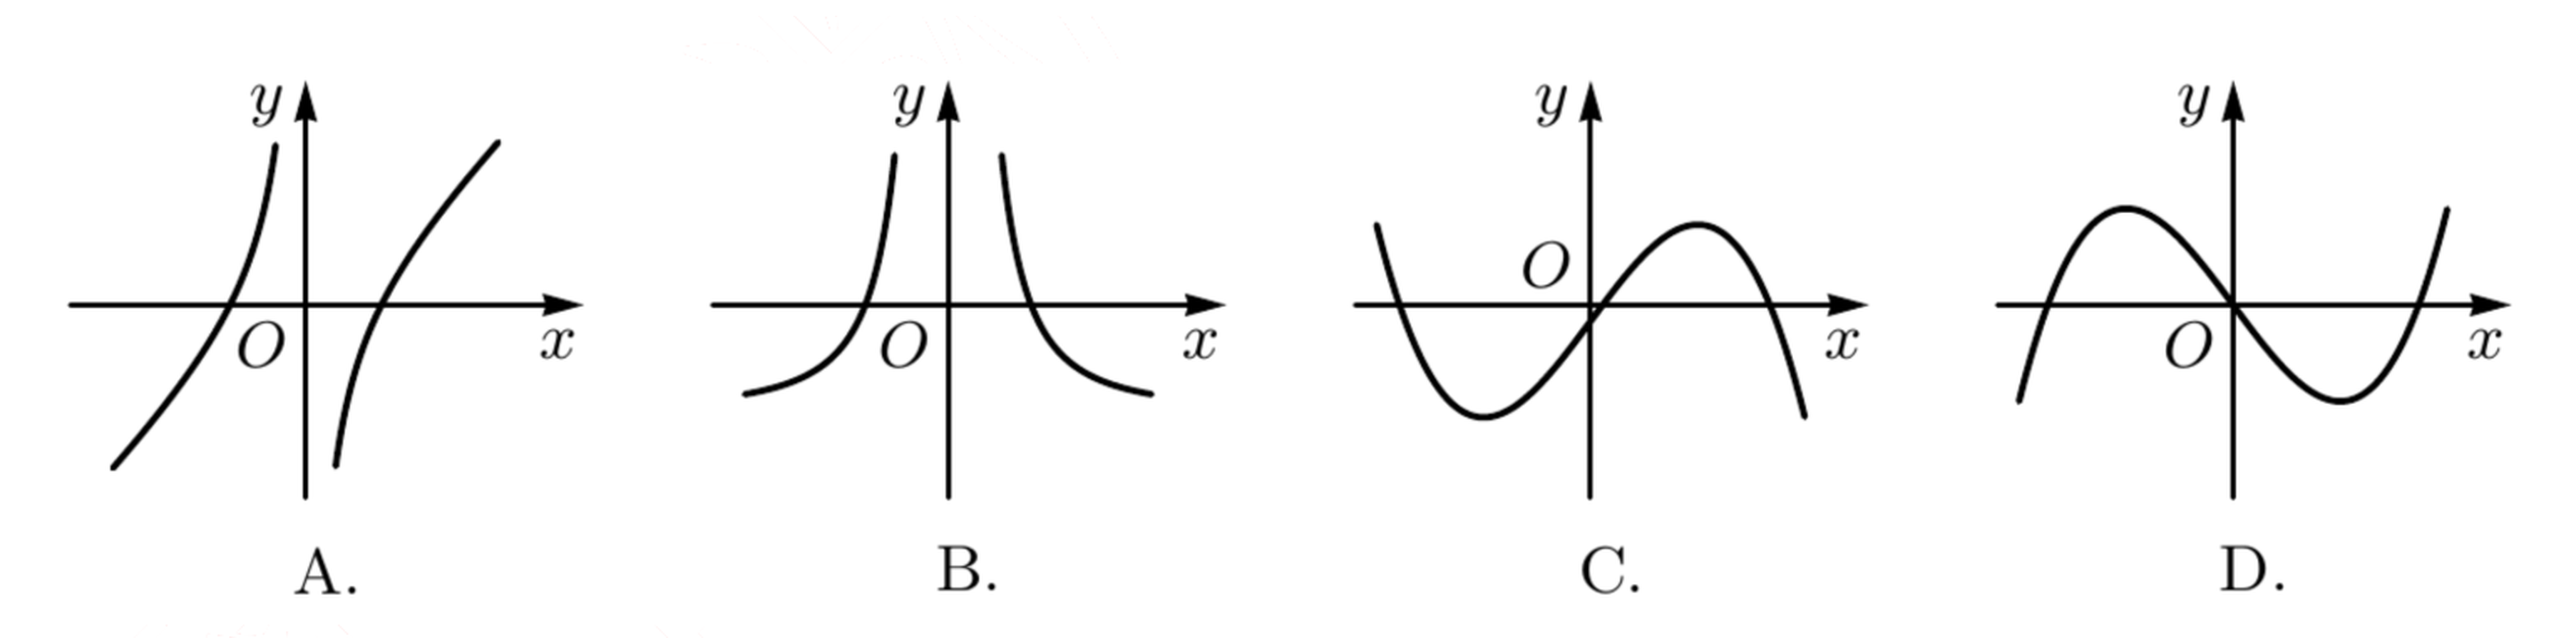
\includegraphics[width=0.90\textwidth]{figures/gao134_q13_options.png}
\end{center}

\ifanswer
\solbegin
\step{$f(x)$ 为偶函数，$g(x)$ 为奇函数，因此 $f(x)g(x)$ 为奇函数，排除 B.}
\step{又 $x=0$ 不在乘积函数的定义域内，其图象在 $y$ 轴上没有点，排除 C、D，}
\step{故选 $A$.}
\solend
\fi

\item 设全集为自然数集 $\N$，$E=\{x\mid x=2n,n\in\N\}$，$F=\{x\mid x=4n,n\in\N\}$，那么集合 $\N$ 可以表示成\mbox{（\quad）}

\keepwithprev
A. $E\cap F$\qquad\qquad B. $\overline{E}\cup F$\qquad\qquad C. $\overline{F}\cup E$\qquad\qquad D. $\overline{E}\cap\overline{F}$

\ifanswer
\solbegin
\step{$F\subseteq E$，所以 $\overline{F}\cup E=\N$，故选 $C$.}
\solend
\fi

\item 已知函数 $y=f(x)$，其中 $f(x)=x^2+bx$，则“$b<0$”是“$f(f(x))$ 的最小值与 $f(x)$ 的最小值相等”的\mbox{（\quad）}

\keepwithprev
A. 充分非必要条件\qquad\qquad B. 必要非充分条件

C. 充分必要条件\qquad\qquad D. 既非充分又非必要条件

\ifanswer
\solbegin
\step{$f(x)=\left(x+\dfrac b2\right)^2-\dfrac{b^2}4$，最小值为 $-\dfrac{b^2}4$，值域为 $\left[-\dfrac{b^2}4,+\infty\right)$.}
\step{当 $b<0$ 时，$-\dfrac b2>0\geqslant-\dfrac{b^2}4$，存在 $x$ 使 $f(x)=-\dfrac b2$，}
\step{从而 $f(f(x))$ 的最小值也为 $-\dfrac{b^2}4$，充分性成立.}
\step{当 $b=0$ 时，$f(x)=x^2$，$f(f(x))=x^4$，两者最小值均为 $0$，必要性不成立.}
\step{故选 $A$.}
\solend
\fi

\item 已知 $a,b,c\in\R$，若存在常数 $M>0$，使得 $a^2+b^2+c^2<M$，则称 $(a,b,c)$ 是有界数组. 对以下两个命题：

①若 $\lvert a^2+b+c\rvert+\lvert a^2+b-c\rvert\leqslant1$，则 $(a,b,c)$ 是有界数组；

②若 $\lvert a^2+b+c\rvert+\lvert a+b^2-c\rvert\leqslant1$，则 $(a,b,c)$ 是有界数组.% ②第二项为 \lvert a+b^2-c\rvert，与①刻意不同，照录

下列判断正确的是\mbox{（\quad）}

\keepwithprev
A. ①和②均为真命题\qquad\qquad B. ①和②均为假命题

C. ①为真命题，②为假命题\qquad D. ①为假命题，②为真命题

\ifanswer
\solbegin
\step{①取 $a=t,b=-t^2,c=0$，条件左端为 $0$，而 $a^2+b^2+c^2=t^2+t^4$ 可任意大，}
\step{故①为假命题.}
\step{②由条件，$a^2+a+b^2+b\leqslant\lvert a^2+b+c\rvert+\lvert a+b^2-c\rvert\leqslant1$.}
\step{由 $(a+1)^2+(b+1)^2\geqslant0$，得 $a^2+b^2\leqslant2(a^2+a+b^2+b)+2\leqslant4$.}
\step{又 $\lvert c\rvert\leqslant\lvert a^2+b+c\rvert+a^2+\lvert b\rvert\leqslant1+4+2=7$，故 $a^2+b^2+c^2\leqslant53<54$，}
\step{可取 $M=54$，故②为真命题.}
\step{故选 $D$.}
\solend
\fi

\end{enumerate}

\bigsec{三、解答题}

\begin{enumerate}
\setcounter{enumi}{16}

\item 已知不等式 $x^2-ax-b<0$ 的解集为 $A$，不等式 $\dfrac{3-2x}{x-1}<0$ 的解集为 $B$.

(1) 若 $a=5$，$b=-6$，求 $A\cap\overline{B}$；

(2) 若 $b=2a^2$，且 $A\cup B=B$，求实数 $a$ 的取值范围.

\ifanswer
\solbegin
\step{(1) 不等式 $\dfrac{3-2x}{x-1}<0$ 等价于 $x<1$ 或 $x>\dfrac32$，}
\step{所以 $B=(-\infty,1)\cup\left(\dfrac32,+\infty\right)$，$\overline{B}=\left[1,\dfrac32\right]$，}
\step{由 $x^2-5x+6=(x-2)(x-3)<0$，得 $A=(2,3)$，因此 $A\cap\overline{B}=\varnothing$.}
\step{(2) $A\cup B=B\Leftrightarrow A\subseteq B$，且 $x^2-ax-2a^2=(x-2a)(x+a)$，}
\step{当 $a=0$ 时，$A=\varnothing$，满足条件.}
\step{当 $a>0$ 时，$A=(-a,2a)$，$-a<0<1$，$A\subseteq B\Leftrightarrow2a\leqslant1$，得 $0<a\leqslant\dfrac12$.}
\step{当 $a<0$ 时，$A=(2a,-a)$，$2a<0<1$，$A\subseteq B\Leftrightarrow-a\leqslant1$，}
\step{得 $-1\leqslant a<0$.}
\step{因此 $a$ 的取值范围为 $\left[-1,\dfrac12\right]$.}
\solend
\fi

\item 为了在夏季降温和冬季供暖时减少能源损耗，房屋的屋顶和外墙需要建造隔热层. 某幢建筑物要建造可使用 $30$ 年的隔热层，每厘米厚的隔热层建造成本为 $9$ 万元. 该建筑物每年的能源消耗费用 $C$（万元）与隔热层厚度 $x$（cm）满足如下关系式：$C=\dfrac{k}{3x+5}$（$0\leqslant x\leqslant10$）. 若不建隔热层，每年能源消耗费用为 $8$ 万元. 设 $y$（万元）为隔热层建造费用与 $30$ 年的能源消耗费用之和.

(1) 求 $k$ 的值及 $y$ 的表达式；

(2) 隔热层修建多厚时，总费用 $y$ 最小？并求最小值.

\ifanswer
\solbegin
\step{(1) 不建隔热层时 $x=0$，$C=8$，所以 $\dfrac k5=8$，得 $k=40$.}
\step{隔热层建造费用为 $9x$ 万元，$30$ 年的能源消耗费用为 $30\times\dfrac{40}{3x+5}$ 万元.}
\step{因此 $y=9x+\dfrac{1200}{3x+5}$，$0\leqslant x\leqslant10$.}
\step{(2) 令 $t=3x+5$，则 $5\leqslant t\leqslant35$，且 $y=3t+\dfrac{1200}{t}-15$，}
\step{因为 $t>0$，由基本不等式得 $y\geqslant2\sqrt{3t\cdot\dfrac{1200}{t}}-15=105$，}
\step{当且仅当 $3t=\dfrac{1200}{t}$，即 $t=20$时取等号，此时 $x=5\in[0,10]$，}% 原卷"20"与"时"之间未留空，照录
\step{所以隔热层厚度为 $5$ cm 时，总费用最小，最小值为 $105$ 万元.}
\solend
\fi

\item 已知 $f(x)=ax^2+\dfrac1x$，其中 $a$ 为常数.

(1) 若 $a\in(1,3)$，判断函数 $y=f(x)$ 在 $[1,2]$ 上的单调性，并用定义证明；

(2) 求函数 $y=f(x)-x-\dfrac1x$ 在 $[1,2]$ 上的最大值 $g(a)$.

\ifanswer
\solbegin
\step{(1) 任取 $x_1,x_2\in[1,2]$，且 $x_1<x_2$，}
\step{则 $f(x_2)-f(x_1)=(x_2-x_1)\left[a(x_1+x_2)-\dfrac1{x_1x_2}\right]$，}
\step{由 $a>1$，$x_1+x_2\geqslant2$，$x_1x_2\geqslant1$，得 $a(x_1+x_2)-\dfrac1{x_1x_2}>2-1>0$，}
\step{因此 $f(x_2)>f(x_1)$，$f(x)$ 在 $[1,2]$ 上为严格增函数.}
\step{(2) 令 $h(x)=f(x)-x-\dfrac1x=ax^2-x$，其中 $x\in[1,2]$.}
\step{若 $a=0$，则 $h(x)=-x$，所以 $h(x)_{max}=h(1)=-1$；}
\step{若 $a<0$，二次函数的图象的对称轴为 $x=\dfrac1{2a}<0$，}
\step{所以 $y=h(x)$ 在 $[1,2]$ 上是严格减函数，所以 $h(x)_{max}=h(1)=a-1$；}
\step{若 $a>0$ 且 $\dfrac1{2a}>\dfrac32$，即 $0<a<\dfrac13$ 时，$h(x)_{max}=h(1)=a-1$.}
\step{若 $a>0$ 且 $\dfrac1{2a}\leqslant\dfrac32$，即 $a\geqslant\dfrac13$ 时，$h(x)_{max}=h(2)=4a-2$.}
\step{综上所述，$g(a)=\begin{cases}a-1,a<\dfrac13\\4a-2,a\geqslant\dfrac13\end{cases}$.}
\solend
\fi

\item 已知 $f(x)=\dfrac{ax^2+1}{bx+c}$（$a,b,c\in\Z$）.

(1) 若函数 $y=f(x)$ 是奇函数，且 $f(1)=2$，$f(2)<3$，求 $a,b,c$ 的值；

(2) 若函数 $y=f(x)$ 是偶函数，且 $ac<0$，$f(2a^2+a+1)<f(-3a^2+2a-1)$，求 $a$ 的值；

(3) 若 $b=a+c^2$，且满足不等式 $\lvert f(x)\rvert\geqslant1$ 的 $x$ 的最大值为 $0$，求 $c$ 的值.

\ifanswer
\solbegin
\step{(1) 由 $f(-x)=-f(x)$，交叉相乘得 $2c(ax^2+1)=0$ 恒成立，}
\step{因此 $c=0$，$b\neq0$.}
\step{由 $f(1)=2$，得 $a+1=2b$，}
\step{于是 $f(2)=\dfrac{4a+1}{2b}=4-\dfrac3{2b}<3\Leftrightarrow0<b<\dfrac32$，}
\step{因为 $b\in\Z$，所以 $b=1$，进而 $a=1$，$c=0$.}
\step{(2) 由 $f(-x)=f(x)$，交叉相乘得 $2bx(ax^2+1)=0$ 恒成立，因此 $b=0$.}
\step{此时 $f(x)=\dfrac ac x^2+\dfrac1c$，且 $\dfrac ac<0$.}
\step{设 $u=2a^2+a+1$，$v=-3a^2+2a-1$.}
\step{方程 $2a^2+a+1=0$ 与 $3a^2-2a+1=0$ 的判别式分别为 $-7$ 与 $-8$，}
\step{都小于 $0$，所以 $u>0$，$v<0$.}
\step{于是 $f(u)<f(v)\Leftrightarrow u^2>v^2\Leftrightarrow u>-v\Leftrightarrow-a^2+3a>0\Leftrightarrow0<a<3$，}
\step{因为 $a\in\Z$，所以 $a=1$ 或 $a=2$.}
\step{(3) 因为解集的最大值为 $0$，所以 $f(0)$ 有定义且 $\lvert f(0)\rvert\geqslant1$，}
\step{即 $c\neq0$，$\left\lvert\dfrac1c\right\rvert\geqslant1$，结合 $c\in\Z$，得 $c=\pm1$，从而 $b=a+1$.}
\step{当 $x=2$ 时，分母 $2a+2+c$ 为奇数，必不为 $0$；}
\step{又因为 $2>0$，必须有 $\lvert f(2)\rvert<1\Leftrightarrow\lvert4a+1\rvert<\lvert2a+2+c\rvert$，}
\step{若 $c=-1$，则 $(4a+1)^2<(2a+1)^2\Leftrightarrow4a(3a+1)<0\Leftrightarrow-\dfrac13<a<0$，}
\step{不存在满足条件的整数 $a$.}
\step{若 $c=1$，则 $(4a+1)^2<(2a+3)^2\Leftrightarrow4(3a+2)(a-1)<0\Leftrightarrow-\dfrac23<a<1$，}
\step{所以 $a=0$，$b=1$，此时 $f(x)=\dfrac1{x+1}$，}
\step{且 $\lvert f(x)\rvert\geqslant1\Leftrightarrow0<\lvert x+1\rvert\leqslant1\Leftrightarrow x\in[-2,-1)\cup(-1,0]$，}
\step{解集的最大值确为 $0$，因此 $c=1$.}
\solend
\fi

\item 已知函数 $y=f(x)$ 的定义域为 $\R$，且当 $x>0$ 时，$f(x)=\dfrac1{x+1}$. 对任意 $x_0\in\R$，定义集合 $D(x_0)=\{d\mid f(x_0+d)>f(x_0)\}$.

(1) 若当 $x\leqslant0$ 时，$f(x)=-2x+1$，求函数 $y=f(x)$ 的值域；

(2) 若 $y=f(x)$ 是偶函数，且 $f(0)=1$，求证：$D(-2)=\{-d\mid d\in D(2)\}$；

(3) 若 $y=f(x)$ 是奇函数，且 $x_1x_2\neq0$，求证：“$f(x_1)\leqslant f(x_2)$”的充要条件是\!\mbox{“$D(x_2)\subseteq D(x_1)$”}.

\ifanswer
\solbegin
\step{(1) 当 $x>0$ 时，$0<f(x)<1$；当 $x\leqslant0$ 时，$f(x)=-2x+1\geqslant1$.}
\step{函数的值域为 $(0,1)\cup[1,+\infty)=(0,+\infty)$.}
\step{(2) 由 $f(x)$ 是偶函数及 $f(0)=1$，得 $f(x)=\dfrac1{1+\lvert x\rvert}$，且 $f(2)=f(-2)=\dfrac13$.}
\stepm{法一：}{$D(2)=\left\{d\mid\dfrac1{1+\lvert2+d\rvert}>\dfrac13\right\}=\{d\mid\lvert2+d\rvert<2\}=(-4,0)$，}
\step{$D(-2)=\left\{d\mid\dfrac1{1+\lvert-2+d\rvert}>\dfrac13\right\}=\{d\mid\lvert-2+d\rvert<2\}=(0,4)$，}
\step{因此 $\{-d\mid d\in D(2)\}=(0,4)=D(-2)$.}
\stepm{法二：}{任取 $d\in D(-2)$，由定义得 $f(-2+d)>f(-2)$.}
\step{因为 $y=f(x)$ 是偶函数，所以对任意的实数 $x$，有 $f(-x)=f(x)$，}
\step{因此 $f(-2+d)=f(-(-2+d))=f(2-d)$，且 $f(-2)=f(2)$.}
\step{所以不等式 $f(-2+d)>f(-2)$ 等价于 $f(2-d)>f(2)$，}
\step{这恰好是 $-d\in D(2)$ 的定义，}
\step{所以 $d\in D(-2)\Leftrightarrow-d\in D(2)$，故 $D(-2)=\{-d\mid d\in D(2)\}$.}
\step{(3) 由 $f(x)$ 是奇函数，得 $f(0)=0$；}
\step{当 $x<0$ 时，$f(x)=-f(-x)=-\dfrac1{1-x}=\dfrac1{x-1}$；}
\step{所以 $f(x)=\begin{cases}\dfrac1{x-1},&x<0\\0,&x=0;\\\dfrac1{x+1},&x>0\end{cases}$}
% 2026-11-15 回原图订正：原卷 11 页此 cases 块末无句点，本稿初转顺手补了西文句点，今删去（Q19 08 页同类块末有句点，照录保留）。
\step{当 $x_0<0$ 时，$D(x_0)=\{d\mid f(x_0+d)>f(x_0)\}=(-\infty,0)\cup[-x_0,+\infty)$，}
\step{当 $x_0=0$ 时，$D(0)=\{d\mid f(0+d)>f(0)\}=(0,+\infty)$，}
\step{当 $x_0>0$ 时，$D(x_0)=\{d\mid f(x_0+d)>f(x_0)\}=(-x_0,0)$.}
\stepm{先证明必要性.}{若 $f(x_1)\leqslant f(x_2)$，仅需讨论三类情形：}
\step{若 $x_2\leqslant x_1<0$，}
\step{则 $D(x_1)=(-\infty,0)\cup[-x_1,+\infty),D(x_2)=(-\infty,0)\cup[-x_2,+\infty)$，}
\step{故 $D(x_2)\subseteq D(x_1)$；}
\step{若 $0<x_2\leqslant x_1$，则 $D(x_1)=(-x_1,0),D(x_2)=(-x_2,0)$，}
\step{故 $D(x_2)\subseteq D(x_1)$；}
\step{若 $x_1<0<x_2$，则 $D(x_1)=(-\infty,0)\cup[-x_1,+\infty),D(x_2)=(-x_2,0)$，}
\step{故 $D(x_2)\subseteq D(x_1)$.}
\stepm{再证明充分性.}{若 $D(x_2)\subseteq D(x_1)$，}
\step{若 $x_1<0,x_2<0$，}
\step{则 $D(x_1)=(-\infty,0)\cup[-x_1,+\infty),D(x_2)=(-\infty,0)\cup[-x_2,+\infty)$，}
\step{由 $D(x_2)\subseteq D(x_1)$ 得 $x_2\leqslant x_1$，}
\step{又 $y=f(x)$ 在 $(-\infty,0)$ 上是严格减函数，所以 $f(x_1)\leqslant f(x_2)$；}
\step{若 $x_1>0,x_2>0$，则 $D(x_1)=(-x_1,0),D(x_2)=(-x_2,0)$，}
\step{由 $D(x_2)\subseteq D(x_1)$ 得 $x_2\leqslant x_1$，}
\step{又 $y=f(x)$ 在 $(0,+\infty)$ 上是严格减函数，所以 $f(x_1)\leqslant f(x_2)$；}
\step{若 $x_1<0,x_2>0$，则 $f(x_1)<0<f(x_2)$，结论成立；}
\step{若 $x_1>0,x_2<0$，此时 $D(x_1)=(-x_1,0)$ 中只有负数，}
\step{而 $D(x_2)=(-\infty,0)\cup[-x_2,+\infty)$ 中有正数，$D(x_2)\subseteq D(x_1)$ 不成立.}
\step{综上，“$f(x_1)\leqslant f(x_2)$”的充要条件是“$D(x_2)\subseteq D(x_1)$”.}
\solend
\fi

\end{enumerate}

\end{document}
"
% 紧凑版：xelatex "\def\iscompact{1}% 高一134_华师大二附中_期中.tex
%   —— 高一上数学"2026-2027 年华师大二附中高一上期中"（试卷版/答案版）
% 试卷版：xelatex 高一134_华师大二附中_期中.tex
% 答案版：xelatex "\def\isanswer{1}% 高一134_华师大二附中_期中.tex
%   —— 高一上数学"2026-2027 年华师大二附中高一上期中"（试卷版/答案版）
% 试卷版：xelatex 高一134_华师大二附中_期中.tex
% 答案版：xelatex "\def\isanswer{1}% 高一134_华师大二附中_期中.tex
%   —— 高一上数学"2026-2027 年华师大二附中高一上期中"（试卷版/答案版）
% 试卷版：xelatex 高一134_华师大二附中_期中.tex
% 答案版：xelatex "\def\isanswer{1}\input{高一134_华师大二附中_期中.tex}"
% 紧凑版：xelatex "\def\iscompact{1}\input{高一134_华师大二附中_期中.tex}"
%
% ① 原始材料：微信公众号"魔都数学加油站"文章，作者破晓，2026-11-15 18:04 发布；
% 连载"27学年高一134"，原文标题"27学年高一134——2026-2027年上海市华师大二附中高一上期中"；
% 原文链接：https://mp.weixin.qq.com/s/bQlkmlGdCtAlytY331vf3g。
% 正文为 13 张 PNG 页（01、04、06、08、09、10、11、12、13 为 2560x3620；
% 02、03、05、07 为 4762x6735，同一篇各页分辨率不同，逐页按各自分辨率裁图核对），
% 题目下印有【解析】，为讲评版。题目、解析均据原图转录；卷面粉红色水印
% "魔都数学加油站"及公众号页脚未录入。
% 全卷 2 幅插图，均在第 04 页：第 13 题题干 y=f(x)、y=g(x) 两幅函数图象合并裁为
% figures/gao134_q13_graphs.png，第 13 题 A/B/C/D 四幅函数图象选项合并裁为
% figures/gao134_q13_options.png；两图均取原卷 04 页截图 3× LANCZOS 放大、
% 白化粉色水印（只白化浅粉色 R>175 且 G>140 且 B>140 的像素，保留红色标签）。
% 注意：本卷 Q13 四幅选项在原卷排为"一行四幅"（1×4），并非 高一132 第 14 题
% 的 2×2 排布，本稿按原卷 1×4 合并裁为一张，不重排、不用 TikZ 重绘。
%
% 卷首标题：原卷印作"2026-2027 年华师大二附中高一上期中"（公众号标题中的"上海市"
% 卷面标题行没有，本稿照卷面），年份区间按全稿惯例排 en dash；原卷未印副标题，
% 本卷为期中卷、跨集合与常用逻辑用语／不等式／函数三章，按题目内容标为
% "集合与常用逻辑用语、不等式、函数"（与 125／126／128／129／131／132／133 同期中卷口径相同）：
% 集合与逻辑见 Q6、Q10、Q14、Q16、Q17、Q21，不等式见 Q3、Q7、Q9、Q11、Q15、Q18、Q19，
% 函数（函数性质、二分法、奇偶性、基本不等式应用）见 Q4、Q5、Q8、Q12、Q13、Q20。
%
% 题号体例：本卷共 19 题——一、填空题 3—12（10 题）、二、选择题 13—16（4 题）、
% 三、解答题 17—21（5 题）。三节分别 \setcounter{enumi}{2}／{12}／{16}。
% 第 13 页仅为 Q21 (3) 解析续尾，全卷无「四、附加题」。
%
% ② 与原卷的排版差异：
%   ① 原文从第 3 题起，本稿保留原题号（见上"题号体例"）；
%   ② 原卷每题下直接印【解析】，本稿按全稿惯例置于答案版；第 13—16 题答案均在
%      解析末句"故选 …"，题干括号内留空、不另提 \ans{}（四题均无独立答案段）；
%      全卷无只印括号内答案、无解析的选择题；
%   ③ 原卷未印副标题，本稿按"知识模块"口径补出；
%   ④ 原卷填空横线按全稿惯例排为 \blankline[4.4em]；选择题括号排 \mbox{（\quad）}、
%      每个选项段前按惯例加 \keepwithprev（Q13 四选项为图，守卫前行为 \begin{center}；
%      Q15、Q16 四选项分两行排，\keepwithprev 只加在 A. 行前）；解答题不留作答区、
%      不加 \anspace（原卷为讲评版，与 129／131／132／133 同）；
%   ⑤ 原卷数集印黑板粗体（Q7／Q11／Q12／Q16／Q21 的 R、Q14／Q20 的 N、Q20 的 Z），
%      按全稿惯例统一排 \R／\N／\Z；绝对值排 \lvert…\rvert，集合描述竖线排 \mid；不等号按全稿惯例排
%      \leqslant／\geqslant；补集照原卷上划线排 \overline{B}、\overline{E}、\overline{F}；
%   ⑥ 子题标号 (1)(2)(3) 与括注原卷均用半角括号，照录（与 131／132／133 同）；
%      圈数字 ①② 照录；原卷 Q21 (2) 解析"法一：""法二："与 Q21 (3) 解析
%      "先证明必要性.""再证明充分性."四处标签印红色加粗，按 高一53／108／133 成例排
%      \stepm{法一：}／\stepm{法二：}／\stepm{先证明必要性.}／\stepm{再证明充分性.}
%      （加粗着色、不引入红色，不动 common.sty）；Q8 解析"第 1 步：""第 2 步：""
%      "第 3 步："原卷印黑色常规宋体（非红非粗），照录为普通 \step 行内文字；
%   ⑦ 数学式内半角逗号照录（如 Q6 $A=\{0,1,2,3\}$、Q14 $x=2n,n\in\N$、
%      Q16 $a,b,c\in\R$ 与 $a=t,b=-t^2,c=0$、Q19 $x_1,x_2\in[1,2]$、
%      Q20 $a,b,c\in\Z$、Q21 $x_1<0,x_2<0$ 与 $D(x_1)=(-x_1,0),D(x_2)=(-x_2,0)$）；
%      原卷行末全角句点按全稿惯例从宽排西文句点；cases 块末的句点逐处照录：
%      Q19 解析（08 页）块末原卷有句点照录、Q21 (3) 解析（11 页）块末原卷无句点不补，
%      两处原卷自身不统一（2026-11-15 回原图核对，本稿初转曾顺手补句点，已删去）；
%   ⑧ 原卷 Q8 解析跨 01—02 页、Q10 解析跨 02—03 页、Q12 解析跨 03—04 页、
%      Q16 解析跨 05—06 页、Q17 解析跨 06—07 页、Q20 解析跨 08—10 页、
%      Q21 解析跨 10—13 页，本稿按题合并连续排版；末页第 13 页为
%      Q21 (3) 解析续尾与"综上"一句，按实际印刷行单列；
%   ⑨ 题干中的中文弯引号按原卷照录（Q10 研究问题、Q15 条件、Q21 (3) 充要条件），
%      注释内一律 ASCII 引号。
%
% 判别式字形：全卷仅 Q9 解析末行出现一处判别式记号
%   "两值均满足 $\Delta=p^2-4p=18\mp12\sqrt2>0$"，逐处放大核对，原卷印高三角
%   $\Delta$（等腰、高，实测高宽比约 1.14），照录 \Delta；卷内无扁三角 \triangle，
%   与 高一132 同题排 $\triangle$、高一133 部分判别式排 $\triangle$ 均不同。
%
% 子集符号：Q6 题干 $C\subseteq A$、$C\subseteq B$ 与解析 $C\subseteq A\cap B$、
%   Q14 解析 $F\subseteq E$、Q17 解析 $A\subseteq B$、Q21 题干与解析各处的
%   $D(x_2)\subseteq D(x_1)$，全部印带下划线的 $\subseteq$，逐处放大核对，
%   照录 \subseteq；全卷未出现单线 \subset。
%
% 原卷存疑照录（均照录未改，正文对应处另有 % 注）：
%   第 6 题题干集合 $A=\{0,1,2,3\}$ 三个逗号后不留空，紧邻的 $B=\{0,2,4,5\}$
%      三个逗号后却留空，同卷同一行两集合排字不一，照录其逗号均为半角；
%   第 16 题命题②作 $\lvert a^2+b+c\rvert+\lvert a+b^2-c\rvert\leqslant1$，
%      与命题①第二项 $\lvert a^2+b-c\rvert$ 不同（①无 $b$ 的平方、②有），
%      两命题刻意不同，照录；解析"②由条件，$a^2+a+b^2+b\leqslant\cdots$"
%      由两项相加直接得到，照录；
%   第 18 题 (2) 解析"即 $t=20$时取等号"中"20"与"时"之间原卷未留空，照录；
%   第 19 题解析 $h(x)_{max}$ 的"max"下标三处字形不一（斜体／正体混排），照录；
%   第 20 题 (1)(2) 解析"由 $f(-x)=-f(x)$，交叉相乘得……"与"由 $f(-x)=f(x)$，
%      交叉相乘得……"两处措辞照录；
%   第 21 题 (2) 原卷并存"法一"（集合计算）与"法二"（定义推证）两套证明，照录不删。
%
% 行数复核：逐题数 \step/\stepm 条数，合计 134 条（Q3：2；Q4：1；Q5：1；Q6：1；
% Q7：2；Q8：4；Q9：3；Q10：4；Q11：5；Q12：8；Q13：3；Q14：1；Q15：5；
% Q16：7；Q17：9；Q18：7；Q19：11；Q20：22；Q21：38），与原卷印刷行逐题相等
% （cases 块作一个印刷行计）。第 13—16 题答案在解析末句，括号内留空、不另提 \ans{}；
% 第 21 题四条 \stepm 计入 38 条内。
%
\documentclass[a4paper,11pt]{article}
\usepackage{common}

\begin{document}

\examtitlest[3]{2026--2027 年华师大二附中高一上期中}{集合与常用逻辑用语、不等式、函数}

\bigsec{一、填空题}

\begin{enumerate}
\setcounter{enumi}{2}

\item 不等式 $\lvert 2x+1\rvert\geqslant3$ 的解集为\blankline[4.4em].

\ifanswer
\solbegin
\step{$\lvert 2x+1\rvert\geqslant3\Leftrightarrow 2x+1\leqslant-3$ 或 $2x+1\geqslant3\Leftrightarrow x\leqslant-2$ 或 $x\geqslant1$，}
\step{故解集为 $(-\infty,-2]\cup[1,+\infty)$.}
\solend
\fi

\item 函数 $y=\sqrt{x+1}+\dfrac1x$ 的定义域为\blankline[4.4em].

\ifanswer
\solbegin
\step{$x+1\geqslant0$ 且 $x\neq0$，得定义域为 $[-1,0)\cup(0,+\infty)$.}
\solend
\fi

\item 已知等式 $3x^2-4x-2=a(x-1)^2+b(x-1)+c$ 恒成立，其中 $a$、$b$、$c$ 为常数，则 $a-b+c=$\blankline[4.4em].

\ifanswer
\solbegin
\step{令 $x=0$，得 $a-b+c=-2$.}
\solend
\fi

\item 已知集合 $A=\{0,1,2,3\}$，$B=\{0,2,4,5\}$，$C\subseteq A$，$C\subseteq B$，符合条件的集合 $C$ 有\blankline[4.4em]个.% 原卷 A 的逗号后不留空、B 的逗号后留空，排字不一，照录

\ifanswer
\solbegin
\step{$C\subseteq A\cap B=\{0,2\}$，所以符合条件的集合 $C$ 有 $2^2=4$ 个.}
\solend
\fi

\item 设 $a$、$b\in\R$，且 $a^2+4b^2=2$，则 $ab$ 的最大值为\blankline[4.4em].

\ifanswer
\solbegin
\step{$(a-2b)^2=a^2+4b^2-4ab=2-4ab\geqslant0$，得 $ab\leqslant\dfrac12$，}
\step{当且仅当 $a=2b=\pm1$ 时取等号，故 $ab$ 的最大值为 $\dfrac12$.}
\solend
\fi

\item 已知函数 $y=x(13-2x)^2-140$，用二分法求函数在区间 $(3,4)$ 上的零点时，第 3 步应计算 $x=$\blankline[4.4em]的函数值.

\ifanswer
\solbegin
\step{记 $f(x)=x(13-2x)^2-140$，则 $f(3)=7>0$，$f(4)=-40<0$.}
\step{第 1 步：$f\left(\dfrac72\right)=-14<0$，区间缩小为 $\left(3,\dfrac72\right)$.}
\step{第 2 步：$f\left(\dfrac{13}4\right)=-\dfrac{43}{16}<0$，区间缩小为 $\left(3,\dfrac{13}4\right)$.}
\step{第 3 步：应计算 $x=\dfrac{3+\frac{13}4}2=\dfrac{25}8$ 的函数值.}
\solend
\fi

\item 已知一元二次方程 $x^2+px+p=0$ 的两个实根分别为 $x_1$、$x_2$，且 $x_1^2x_2+x_2^2x_1=-18$，则 $p=$\blankline[4.4em].% 判别式 \Delta 高三角，逐处放大核对

\ifanswer
\solbegin
\step{由韦达定理，$x_1+x_2=-p$，$x_1x_2=p$，}
\step{则 $x_1^2x_2+x_2^2x_1=x_1x_2(x_1+x_2)=-p^2=-18\Rightarrow p=\pm3\sqrt2$，}
\step{两值均满足 $\Delta=p^2-4p=18\mp12\sqrt2>0$，故 $p=\pm3\sqrt2$.}
\solend
\fi

\item 研究问题：“已知关于 $x$ 的不等式 $ax^2-bx+c>0$ 的解集为 $(1,2)$，解关于 $x$ 的不等式 $cx^2-bx+a>0$”，有如下解法：

解：由 $ax^2-bx+c>0\Rightarrow a-b\left(\dfrac1x\right)+c\left(\dfrac1x\right)^2>0$，令 $y=\dfrac1x$，则 $y\in\left(\dfrac12,1\right)$，

所以不等式 $cx^2-bx+a>0$ 的解集为 $\left(\dfrac12,1\right)$.

参考上述解法，已知关于 $x$ 的不等式 $\dfrac{k}{x+a}+\dfrac{x+b}{x+c}<0$ 的解集为 $(-3,-1)\cup(2,4)$，则关于 $x$ 的不等式 $\dfrac{kx}{ax-1}+\dfrac{bx-1}{cx-1}<0$ 的解集为\blankline[4.4em].

\ifanswer
\solbegin
\step{当 $x=0$ 时，所求不等式左端为 $1$，不满足不等式.}
\step{当 $x\neq0$ 时，两个分式的分子、分母同除以 $x$，得 $\dfrac{k}{a-\frac1x}+\dfrac{b-\frac1x}{c-\frac1x}<0$.}
\step{令 $t=-\dfrac1x$，则所求不等式化为 $\dfrac{k}{t+a}+\dfrac{t+b}{t+c}<0$，即 $-\dfrac1x\in(-3,-1)\cup(2,4)$，}
\step{解得 $x\in\left(-\dfrac12,-\dfrac14\right)\cup\left(\dfrac13,1\right)$.}
\solend
\fi

\item 已知 $a\in(0,+\infty)$，若对任意的 $x\in(0,+\infty)$，均有 $\lvert x^2-a\rvert+\lvert x+b\rvert=\lvert x^2+x-a+b\rvert$，则 $a^2-b^2$ 的最小值为\blankline[4.4em].

\ifanswer
\solbegin
\step{原等式成立的充要条件是 $(x^2-a)(x+b)\geqslant0$.}
\step{当 $0<x<\sqrt a$ 时须有 $x+b\leqslant0$；当 $x>\sqrt a$ 时须有 $x+b\geqslant0$，因此 $b=-\sqrt a$.}
\step{此时 $(x^2-a)(x+b)=(x+\sqrt a)(x-\sqrt a)^2\geqslant0$，满足题意.}
\step{$a^2-b^2=a^2-a=\left(a-\dfrac12\right)^2-\dfrac14\geqslant-\dfrac14$，}
\step{当 $a=\dfrac12$，$b=-\dfrac{\sqrt2}2$ 时取等号，最小值为 $-\dfrac14$.}
\solend
\fi

\item 已知函数 $y=f(x)$ 在 $\R$ 上是严格增函数，当 $x\neq0$ 且 $f(x)\neq0$ 时，满足 $f(x)\cdot f\left[\dfrac1{f(x)}+\dfrac1x\right]=1$，则 $f(1)=$\blankline[4.4em].

\ifanswer
\solbegin
\step{当 $xf(x)>0$ 时，记 $t=\dfrac1{f(x)}+\dfrac1x\neq0$，则 $f(t)=\dfrac1{f(x)}\neq0$.}
\step{将 $t$ 代入题设，得 $f\left(f(x)+\dfrac1t\right)=f(x)$，严格增性给出 $f(x)+\dfrac1t=x$，}
\step{化简得 $f(x)^2+xf(x)-x^2=0$，由 $\dfrac{f(x)}x>0$ 得 $f(x)=\dfrac{\sqrt5-1}2x$.}
\step{设 $a=f(0)$，若 $a>0$，则 $f(a)>f(0)=a>0$；}
\step{若 $a<0$，则 $f(a)<f(0)=a<0$.}
\step{两种情形都有 $af(a)>0$ 且 $\dfrac{f(a)}a>1$，与上式 $\dfrac{f(a)}a=\dfrac{\sqrt5-1}2<1$ 矛盾，}
\step{因此 $f(0)=0$.}
\step{于是 $f(1)>0$，代入上式得 $f(1)=\dfrac{\sqrt5-1}2$.}
\solend
\fi

\end{enumerate}

% 第 13 题是"节标题 + 题干 + 两幅图 + 四幅选项图"约 15cm 的整块，
% 守卫只放在 \bigsec 之前；若再在 \item 之前放第二枚，会在标题已印出后才触发换页，
% 把题目推走、留下孤立节标题（切页审计 B 类）。高度须覆盖整块。
\needvspace{16cm}
\bigsec{二、选择题}

\begin{enumerate}
\setcounter{enumi}{12}

\item 已知函数 $y=f(x)$ 与 $y=g(x)$ 的图象如图所示，则函数 $y=f(x)\cdot g(x)$ 的图象可能是\mbox{（\quad）}

\keepwithprev
\begin{center}
% 题干 y=f(x)、y=g(x) 两幅函数图象取原卷 04 页截图去粉色水印，按原卷左右排布合并为一张
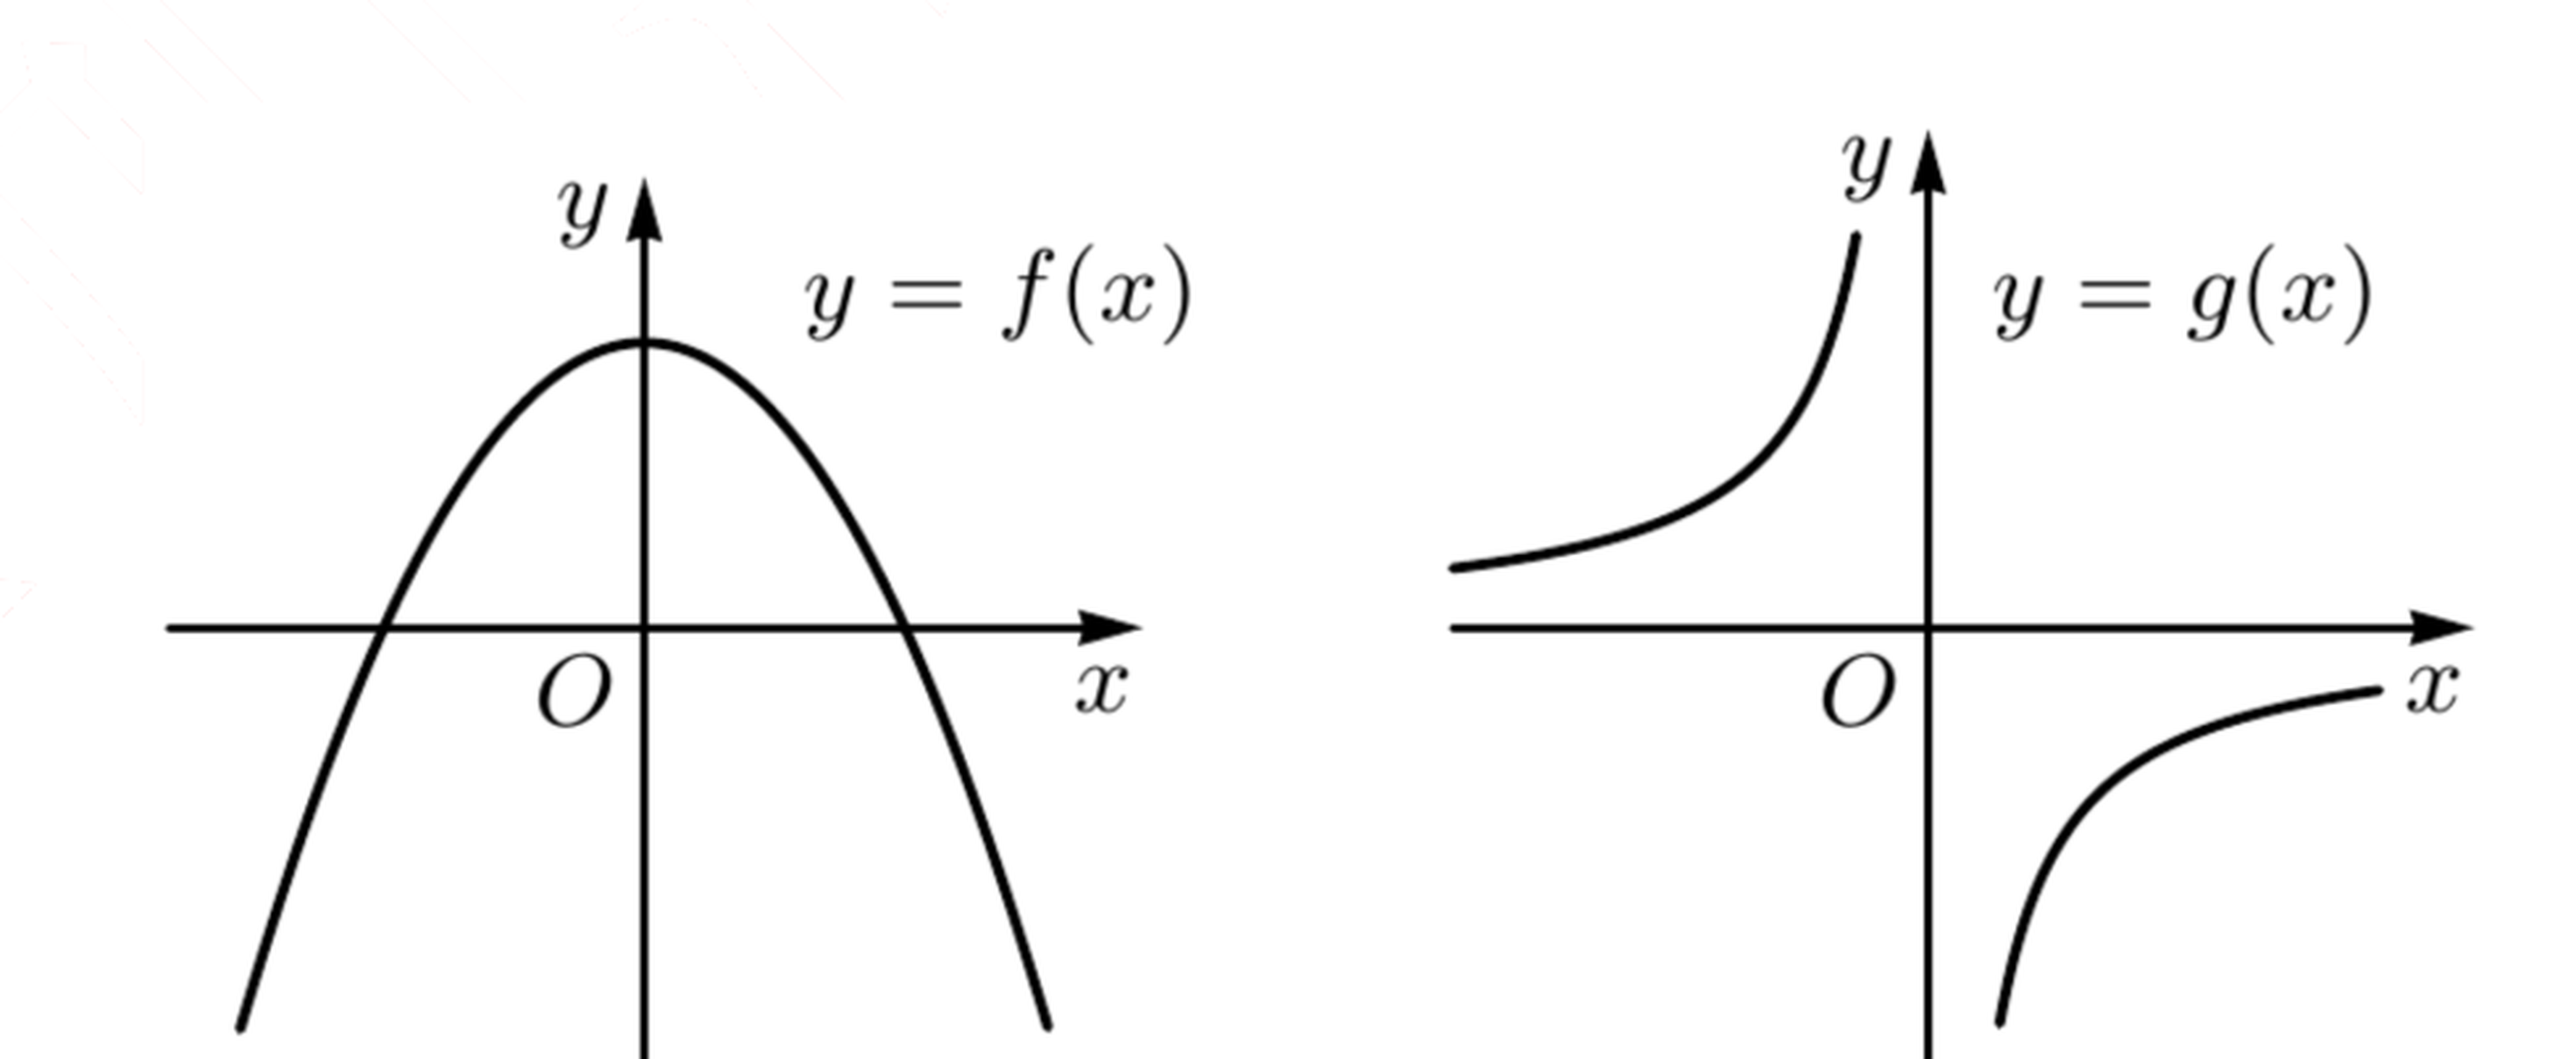
\includegraphics[width=0.72\textwidth]{figures/gao134_q13_graphs.png}\\[0.6em]
% A/B/C/D 四幅函数图象选项取原卷 04 页截图去粉色水印，按原卷一行四幅排布合并为一张
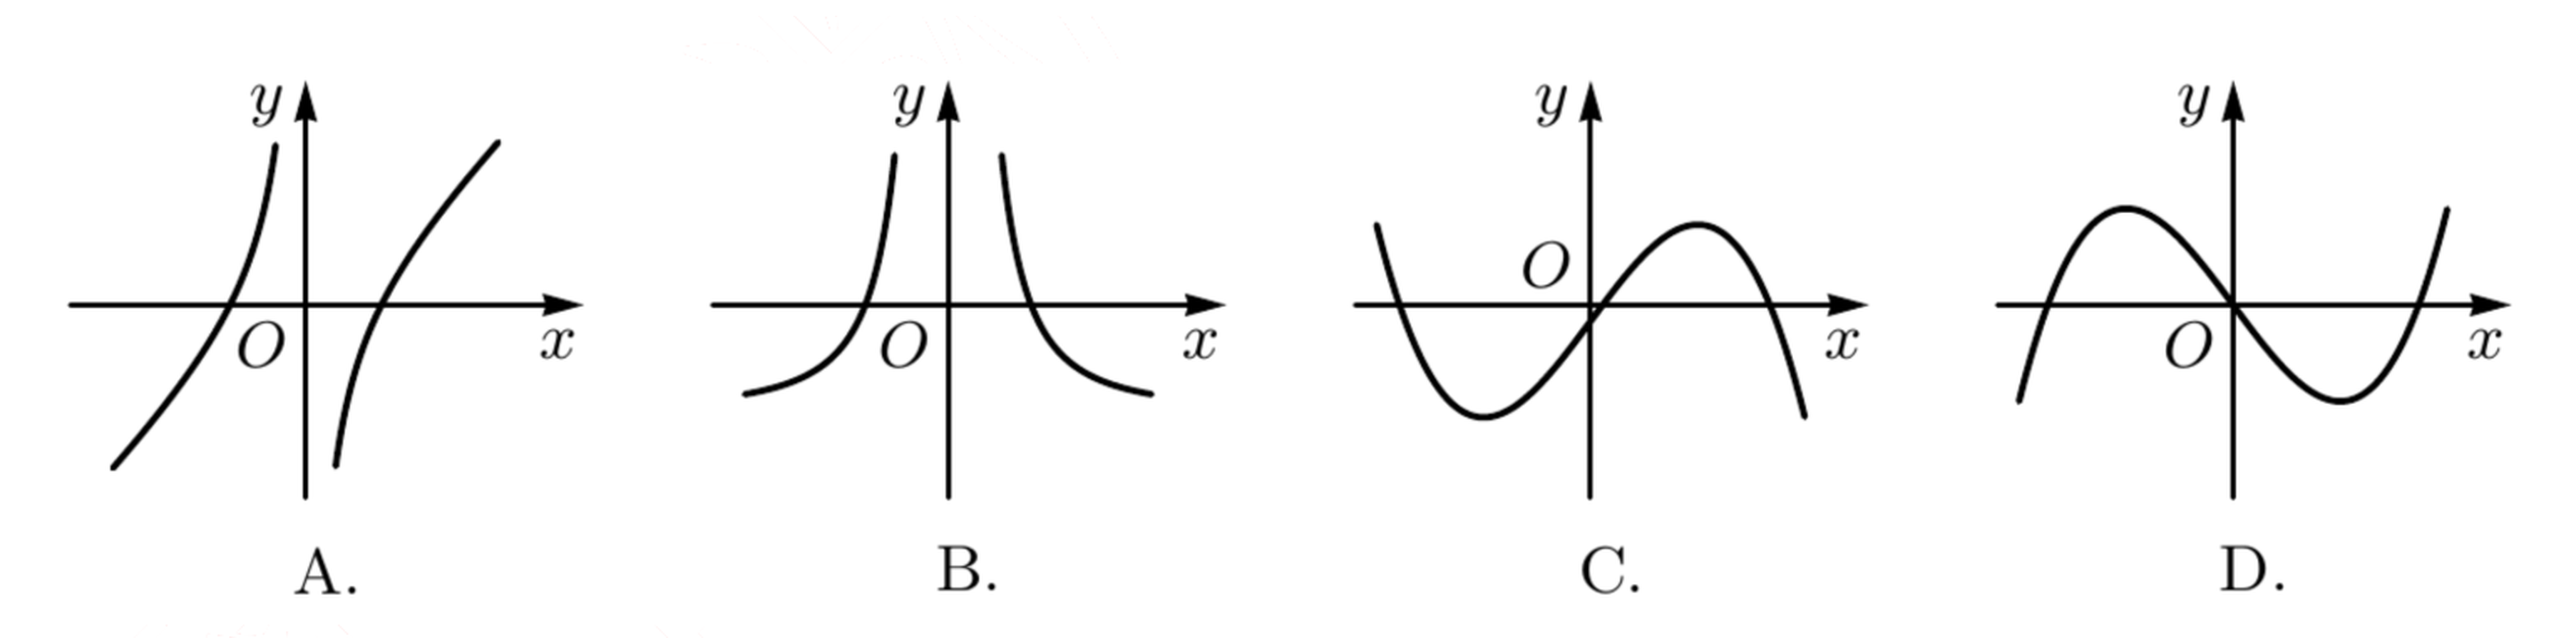
\includegraphics[width=0.90\textwidth]{figures/gao134_q13_options.png}
\end{center}

\ifanswer
\solbegin
\step{$f(x)$ 为偶函数，$g(x)$ 为奇函数，因此 $f(x)g(x)$ 为奇函数，排除 B.}
\step{又 $x=0$ 不在乘积函数的定义域内，其图象在 $y$ 轴上没有点，排除 C、D，}
\step{故选 $A$.}
\solend
\fi

\item 设全集为自然数集 $\N$，$E=\{x\mid x=2n,n\in\N\}$，$F=\{x\mid x=4n,n\in\N\}$，那么集合 $\N$ 可以表示成\mbox{（\quad）}

\keepwithprev
A. $E\cap F$\qquad\qquad B. $\overline{E}\cup F$\qquad\qquad C. $\overline{F}\cup E$\qquad\qquad D. $\overline{E}\cap\overline{F}$

\ifanswer
\solbegin
\step{$F\subseteq E$，所以 $\overline{F}\cup E=\N$，故选 $C$.}
\solend
\fi

\item 已知函数 $y=f(x)$，其中 $f(x)=x^2+bx$，则“$b<0$”是“$f(f(x))$ 的最小值与 $f(x)$ 的最小值相等”的\mbox{（\quad）}

\keepwithprev
A. 充分非必要条件\qquad\qquad B. 必要非充分条件

C. 充分必要条件\qquad\qquad D. 既非充分又非必要条件

\ifanswer
\solbegin
\step{$f(x)=\left(x+\dfrac b2\right)^2-\dfrac{b^2}4$，最小值为 $-\dfrac{b^2}4$，值域为 $\left[-\dfrac{b^2}4,+\infty\right)$.}
\step{当 $b<0$ 时，$-\dfrac b2>0\geqslant-\dfrac{b^2}4$，存在 $x$ 使 $f(x)=-\dfrac b2$，}
\step{从而 $f(f(x))$ 的最小值也为 $-\dfrac{b^2}4$，充分性成立.}
\step{当 $b=0$ 时，$f(x)=x^2$，$f(f(x))=x^4$，两者最小值均为 $0$，必要性不成立.}
\step{故选 $A$.}
\solend
\fi

\item 已知 $a,b,c\in\R$，若存在常数 $M>0$，使得 $a^2+b^2+c^2<M$，则称 $(a,b,c)$ 是有界数组. 对以下两个命题：

①若 $\lvert a^2+b+c\rvert+\lvert a^2+b-c\rvert\leqslant1$，则 $(a,b,c)$ 是有界数组；

②若 $\lvert a^2+b+c\rvert+\lvert a+b^2-c\rvert\leqslant1$，则 $(a,b,c)$ 是有界数组.% ②第二项为 \lvert a+b^2-c\rvert，与①刻意不同，照录

下列判断正确的是\mbox{（\quad）}

\keepwithprev
A. ①和②均为真命题\qquad\qquad B. ①和②均为假命题

C. ①为真命题，②为假命题\qquad D. ①为假命题，②为真命题

\ifanswer
\solbegin
\step{①取 $a=t,b=-t^2,c=0$，条件左端为 $0$，而 $a^2+b^2+c^2=t^2+t^4$ 可任意大，}
\step{故①为假命题.}
\step{②由条件，$a^2+a+b^2+b\leqslant\lvert a^2+b+c\rvert+\lvert a+b^2-c\rvert\leqslant1$.}
\step{由 $(a+1)^2+(b+1)^2\geqslant0$，得 $a^2+b^2\leqslant2(a^2+a+b^2+b)+2\leqslant4$.}
\step{又 $\lvert c\rvert\leqslant\lvert a^2+b+c\rvert+a^2+\lvert b\rvert\leqslant1+4+2=7$，故 $a^2+b^2+c^2\leqslant53<54$，}
\step{可取 $M=54$，故②为真命题.}
\step{故选 $D$.}
\solend
\fi

\end{enumerate}

\bigsec{三、解答题}

\begin{enumerate}
\setcounter{enumi}{16}

\item 已知不等式 $x^2-ax-b<0$ 的解集为 $A$，不等式 $\dfrac{3-2x}{x-1}<0$ 的解集为 $B$.

(1) 若 $a=5$，$b=-6$，求 $A\cap\overline{B}$；

(2) 若 $b=2a^2$，且 $A\cup B=B$，求实数 $a$ 的取值范围.

\ifanswer
\solbegin
\step{(1) 不等式 $\dfrac{3-2x}{x-1}<0$ 等价于 $x<1$ 或 $x>\dfrac32$，}
\step{所以 $B=(-\infty,1)\cup\left(\dfrac32,+\infty\right)$，$\overline{B}=\left[1,\dfrac32\right]$，}
\step{由 $x^2-5x+6=(x-2)(x-3)<0$，得 $A=(2,3)$，因此 $A\cap\overline{B}=\varnothing$.}
\step{(2) $A\cup B=B\Leftrightarrow A\subseteq B$，且 $x^2-ax-2a^2=(x-2a)(x+a)$，}
\step{当 $a=0$ 时，$A=\varnothing$，满足条件.}
\step{当 $a>0$ 时，$A=(-a,2a)$，$-a<0<1$，$A\subseteq B\Leftrightarrow2a\leqslant1$，得 $0<a\leqslant\dfrac12$.}
\step{当 $a<0$ 时，$A=(2a,-a)$，$2a<0<1$，$A\subseteq B\Leftrightarrow-a\leqslant1$，}
\step{得 $-1\leqslant a<0$.}
\step{因此 $a$ 的取值范围为 $\left[-1,\dfrac12\right]$.}
\solend
\fi

\item 为了在夏季降温和冬季供暖时减少能源损耗，房屋的屋顶和外墙需要建造隔热层. 某幢建筑物要建造可使用 $30$ 年的隔热层，每厘米厚的隔热层建造成本为 $9$ 万元. 该建筑物每年的能源消耗费用 $C$（万元）与隔热层厚度 $x$（cm）满足如下关系式：$C=\dfrac{k}{3x+5}$（$0\leqslant x\leqslant10$）. 若不建隔热层，每年能源消耗费用为 $8$ 万元. 设 $y$（万元）为隔热层建造费用与 $30$ 年的能源消耗费用之和.

(1) 求 $k$ 的值及 $y$ 的表达式；

(2) 隔热层修建多厚时，总费用 $y$ 最小？并求最小值.

\ifanswer
\solbegin
\step{(1) 不建隔热层时 $x=0$，$C=8$，所以 $\dfrac k5=8$，得 $k=40$.}
\step{隔热层建造费用为 $9x$ 万元，$30$ 年的能源消耗费用为 $30\times\dfrac{40}{3x+5}$ 万元.}
\step{因此 $y=9x+\dfrac{1200}{3x+5}$，$0\leqslant x\leqslant10$.}
\step{(2) 令 $t=3x+5$，则 $5\leqslant t\leqslant35$，且 $y=3t+\dfrac{1200}{t}-15$，}
\step{因为 $t>0$，由基本不等式得 $y\geqslant2\sqrt{3t\cdot\dfrac{1200}{t}}-15=105$，}
\step{当且仅当 $3t=\dfrac{1200}{t}$，即 $t=20$时取等号，此时 $x=5\in[0,10]$，}% 原卷"20"与"时"之间未留空，照录
\step{所以隔热层厚度为 $5$ cm 时，总费用最小，最小值为 $105$ 万元.}
\solend
\fi

\item 已知 $f(x)=ax^2+\dfrac1x$，其中 $a$ 为常数.

(1) 若 $a\in(1,3)$，判断函数 $y=f(x)$ 在 $[1,2]$ 上的单调性，并用定义证明；

(2) 求函数 $y=f(x)-x-\dfrac1x$ 在 $[1,2]$ 上的最大值 $g(a)$.

\ifanswer
\solbegin
\step{(1) 任取 $x_1,x_2\in[1,2]$，且 $x_1<x_2$，}
\step{则 $f(x_2)-f(x_1)=(x_2-x_1)\left[a(x_1+x_2)-\dfrac1{x_1x_2}\right]$，}
\step{由 $a>1$，$x_1+x_2\geqslant2$，$x_1x_2\geqslant1$，得 $a(x_1+x_2)-\dfrac1{x_1x_2}>2-1>0$，}
\step{因此 $f(x_2)>f(x_1)$，$f(x)$ 在 $[1,2]$ 上为严格增函数.}
\step{(2) 令 $h(x)=f(x)-x-\dfrac1x=ax^2-x$，其中 $x\in[1,2]$.}
\step{若 $a=0$，则 $h(x)=-x$，所以 $h(x)_{max}=h(1)=-1$；}
\step{若 $a<0$，二次函数的图象的对称轴为 $x=\dfrac1{2a}<0$，}
\step{所以 $y=h(x)$ 在 $[1,2]$ 上是严格减函数，所以 $h(x)_{max}=h(1)=a-1$；}
\step{若 $a>0$ 且 $\dfrac1{2a}>\dfrac32$，即 $0<a<\dfrac13$ 时，$h(x)_{max}=h(1)=a-1$.}
\step{若 $a>0$ 且 $\dfrac1{2a}\leqslant\dfrac32$，即 $a\geqslant\dfrac13$ 时，$h(x)_{max}=h(2)=4a-2$.}
\step{综上所述，$g(a)=\begin{cases}a-1,a<\dfrac13\\4a-2,a\geqslant\dfrac13\end{cases}$.}
\solend
\fi

\item 已知 $f(x)=\dfrac{ax^2+1}{bx+c}$（$a,b,c\in\Z$）.

(1) 若函数 $y=f(x)$ 是奇函数，且 $f(1)=2$，$f(2)<3$，求 $a,b,c$ 的值；

(2) 若函数 $y=f(x)$ 是偶函数，且 $ac<0$，$f(2a^2+a+1)<f(-3a^2+2a-1)$，求 $a$ 的值；

(3) 若 $b=a+c^2$，且满足不等式 $\lvert f(x)\rvert\geqslant1$ 的 $x$ 的最大值为 $0$，求 $c$ 的值.

\ifanswer
\solbegin
\step{(1) 由 $f(-x)=-f(x)$，交叉相乘得 $2c(ax^2+1)=0$ 恒成立，}
\step{因此 $c=0$，$b\neq0$.}
\step{由 $f(1)=2$，得 $a+1=2b$，}
\step{于是 $f(2)=\dfrac{4a+1}{2b}=4-\dfrac3{2b}<3\Leftrightarrow0<b<\dfrac32$，}
\step{因为 $b\in\Z$，所以 $b=1$，进而 $a=1$，$c=0$.}
\step{(2) 由 $f(-x)=f(x)$，交叉相乘得 $2bx(ax^2+1)=0$ 恒成立，因此 $b=0$.}
\step{此时 $f(x)=\dfrac ac x^2+\dfrac1c$，且 $\dfrac ac<0$.}
\step{设 $u=2a^2+a+1$，$v=-3a^2+2a-1$.}
\step{方程 $2a^2+a+1=0$ 与 $3a^2-2a+1=0$ 的判别式分别为 $-7$ 与 $-8$，}
\step{都小于 $0$，所以 $u>0$，$v<0$.}
\step{于是 $f(u)<f(v)\Leftrightarrow u^2>v^2\Leftrightarrow u>-v\Leftrightarrow-a^2+3a>0\Leftrightarrow0<a<3$，}
\step{因为 $a\in\Z$，所以 $a=1$ 或 $a=2$.}
\step{(3) 因为解集的最大值为 $0$，所以 $f(0)$ 有定义且 $\lvert f(0)\rvert\geqslant1$，}
\step{即 $c\neq0$，$\left\lvert\dfrac1c\right\rvert\geqslant1$，结合 $c\in\Z$，得 $c=\pm1$，从而 $b=a+1$.}
\step{当 $x=2$ 时，分母 $2a+2+c$ 为奇数，必不为 $0$；}
\step{又因为 $2>0$，必须有 $\lvert f(2)\rvert<1\Leftrightarrow\lvert4a+1\rvert<\lvert2a+2+c\rvert$，}
\step{若 $c=-1$，则 $(4a+1)^2<(2a+1)^2\Leftrightarrow4a(3a+1)<0\Leftrightarrow-\dfrac13<a<0$，}
\step{不存在满足条件的整数 $a$.}
\step{若 $c=1$，则 $(4a+1)^2<(2a+3)^2\Leftrightarrow4(3a+2)(a-1)<0\Leftrightarrow-\dfrac23<a<1$，}
\step{所以 $a=0$，$b=1$，此时 $f(x)=\dfrac1{x+1}$，}
\step{且 $\lvert f(x)\rvert\geqslant1\Leftrightarrow0<\lvert x+1\rvert\leqslant1\Leftrightarrow x\in[-2,-1)\cup(-1,0]$，}
\step{解集的最大值确为 $0$，因此 $c=1$.}
\solend
\fi

\item 已知函数 $y=f(x)$ 的定义域为 $\R$，且当 $x>0$ 时，$f(x)=\dfrac1{x+1}$. 对任意 $x_0\in\R$，定义集合 $D(x_0)=\{d\mid f(x_0+d)>f(x_0)\}$.

(1) 若当 $x\leqslant0$ 时，$f(x)=-2x+1$，求函数 $y=f(x)$ 的值域；

(2) 若 $y=f(x)$ 是偶函数，且 $f(0)=1$，求证：$D(-2)=\{-d\mid d\in D(2)\}$；

(3) 若 $y=f(x)$ 是奇函数，且 $x_1x_2\neq0$，求证：“$f(x_1)\leqslant f(x_2)$”的充要条件是\!\mbox{“$D(x_2)\subseteq D(x_1)$”}.

\ifanswer
\solbegin
\step{(1) 当 $x>0$ 时，$0<f(x)<1$；当 $x\leqslant0$ 时，$f(x)=-2x+1\geqslant1$.}
\step{函数的值域为 $(0,1)\cup[1,+\infty)=(0,+\infty)$.}
\step{(2) 由 $f(x)$ 是偶函数及 $f(0)=1$，得 $f(x)=\dfrac1{1+\lvert x\rvert}$，且 $f(2)=f(-2)=\dfrac13$.}
\stepm{法一：}{$D(2)=\left\{d\mid\dfrac1{1+\lvert2+d\rvert}>\dfrac13\right\}=\{d\mid\lvert2+d\rvert<2\}=(-4,0)$，}
\step{$D(-2)=\left\{d\mid\dfrac1{1+\lvert-2+d\rvert}>\dfrac13\right\}=\{d\mid\lvert-2+d\rvert<2\}=(0,4)$，}
\step{因此 $\{-d\mid d\in D(2)\}=(0,4)=D(-2)$.}
\stepm{法二：}{任取 $d\in D(-2)$，由定义得 $f(-2+d)>f(-2)$.}
\step{因为 $y=f(x)$ 是偶函数，所以对任意的实数 $x$，有 $f(-x)=f(x)$，}
\step{因此 $f(-2+d)=f(-(-2+d))=f(2-d)$，且 $f(-2)=f(2)$.}
\step{所以不等式 $f(-2+d)>f(-2)$ 等价于 $f(2-d)>f(2)$，}
\step{这恰好是 $-d\in D(2)$ 的定义，}
\step{所以 $d\in D(-2)\Leftrightarrow-d\in D(2)$，故 $D(-2)=\{-d\mid d\in D(2)\}$.}
\step{(3) 由 $f(x)$ 是奇函数，得 $f(0)=0$；}
\step{当 $x<0$ 时，$f(x)=-f(-x)=-\dfrac1{1-x}=\dfrac1{x-1}$；}
\step{所以 $f(x)=\begin{cases}\dfrac1{x-1},&x<0\\0,&x=0;\\\dfrac1{x+1},&x>0\end{cases}$}
% 2026-11-15 回原图订正：原卷 11 页此 cases 块末无句点，本稿初转顺手补了西文句点，今删去（Q19 08 页同类块末有句点，照录保留）。
\step{当 $x_0<0$ 时，$D(x_0)=\{d\mid f(x_0+d)>f(x_0)\}=(-\infty,0)\cup[-x_0,+\infty)$，}
\step{当 $x_0=0$ 时，$D(0)=\{d\mid f(0+d)>f(0)\}=(0,+\infty)$，}
\step{当 $x_0>0$ 时，$D(x_0)=\{d\mid f(x_0+d)>f(x_0)\}=(-x_0,0)$.}
\stepm{先证明必要性.}{若 $f(x_1)\leqslant f(x_2)$，仅需讨论三类情形：}
\step{若 $x_2\leqslant x_1<0$，}
\step{则 $D(x_1)=(-\infty,0)\cup[-x_1,+\infty),D(x_2)=(-\infty,0)\cup[-x_2,+\infty)$，}
\step{故 $D(x_2)\subseteq D(x_1)$；}
\step{若 $0<x_2\leqslant x_1$，则 $D(x_1)=(-x_1,0),D(x_2)=(-x_2,0)$，}
\step{故 $D(x_2)\subseteq D(x_1)$；}
\step{若 $x_1<0<x_2$，则 $D(x_1)=(-\infty,0)\cup[-x_1,+\infty),D(x_2)=(-x_2,0)$，}
\step{故 $D(x_2)\subseteq D(x_1)$.}
\stepm{再证明充分性.}{若 $D(x_2)\subseteq D(x_1)$，}
\step{若 $x_1<0,x_2<0$，}
\step{则 $D(x_1)=(-\infty,0)\cup[-x_1,+\infty),D(x_2)=(-\infty,0)\cup[-x_2,+\infty)$，}
\step{由 $D(x_2)\subseteq D(x_1)$ 得 $x_2\leqslant x_1$，}
\step{又 $y=f(x)$ 在 $(-\infty,0)$ 上是严格减函数，所以 $f(x_1)\leqslant f(x_2)$；}
\step{若 $x_1>0,x_2>0$，则 $D(x_1)=(-x_1,0),D(x_2)=(-x_2,0)$，}
\step{由 $D(x_2)\subseteq D(x_1)$ 得 $x_2\leqslant x_1$，}
\step{又 $y=f(x)$ 在 $(0,+\infty)$ 上是严格减函数，所以 $f(x_1)\leqslant f(x_2)$；}
\step{若 $x_1<0,x_2>0$，则 $f(x_1)<0<f(x_2)$，结论成立；}
\step{若 $x_1>0,x_2<0$，此时 $D(x_1)=(-x_1,0)$ 中只有负数，}
\step{而 $D(x_2)=(-\infty,0)\cup[-x_2,+\infty)$ 中有正数，$D(x_2)\subseteq D(x_1)$ 不成立.}
\step{综上，“$f(x_1)\leqslant f(x_2)$”的充要条件是“$D(x_2)\subseteq D(x_1)$”.}
\solend
\fi

\end{enumerate}

\end{document}
"
% 紧凑版：xelatex "\def\iscompact{1}% 高一134_华师大二附中_期中.tex
%   —— 高一上数学"2026-2027 年华师大二附中高一上期中"（试卷版/答案版）
% 试卷版：xelatex 高一134_华师大二附中_期中.tex
% 答案版：xelatex "\def\isanswer{1}\input{高一134_华师大二附中_期中.tex}"
% 紧凑版：xelatex "\def\iscompact{1}\input{高一134_华师大二附中_期中.tex}"
%
% ① 原始材料：微信公众号"魔都数学加油站"文章，作者破晓，2026-11-15 18:04 发布；
% 连载"27学年高一134"，原文标题"27学年高一134——2026-2027年上海市华师大二附中高一上期中"；
% 原文链接：https://mp.weixin.qq.com/s/bQlkmlGdCtAlytY331vf3g。
% 正文为 13 张 PNG 页（01、04、06、08、09、10、11、12、13 为 2560x3620；
% 02、03、05、07 为 4762x6735，同一篇各页分辨率不同，逐页按各自分辨率裁图核对），
% 题目下印有【解析】，为讲评版。题目、解析均据原图转录；卷面粉红色水印
% "魔都数学加油站"及公众号页脚未录入。
% 全卷 2 幅插图，均在第 04 页：第 13 题题干 y=f(x)、y=g(x) 两幅函数图象合并裁为
% figures/gao134_q13_graphs.png，第 13 题 A/B/C/D 四幅函数图象选项合并裁为
% figures/gao134_q13_options.png；两图均取原卷 04 页截图 3× LANCZOS 放大、
% 白化粉色水印（只白化浅粉色 R>175 且 G>140 且 B>140 的像素，保留红色标签）。
% 注意：本卷 Q13 四幅选项在原卷排为"一行四幅"（1×4），并非 高一132 第 14 题
% 的 2×2 排布，本稿按原卷 1×4 合并裁为一张，不重排、不用 TikZ 重绘。
%
% 卷首标题：原卷印作"2026-2027 年华师大二附中高一上期中"（公众号标题中的"上海市"
% 卷面标题行没有，本稿照卷面），年份区间按全稿惯例排 en dash；原卷未印副标题，
% 本卷为期中卷、跨集合与常用逻辑用语／不等式／函数三章，按题目内容标为
% "集合与常用逻辑用语、不等式、函数"（与 125／126／128／129／131／132／133 同期中卷口径相同）：
% 集合与逻辑见 Q6、Q10、Q14、Q16、Q17、Q21，不等式见 Q3、Q7、Q9、Q11、Q15、Q18、Q19，
% 函数（函数性质、二分法、奇偶性、基本不等式应用）见 Q4、Q5、Q8、Q12、Q13、Q20。
%
% 题号体例：本卷共 19 题——一、填空题 3—12（10 题）、二、选择题 13—16（4 题）、
% 三、解答题 17—21（5 题）。三节分别 \setcounter{enumi}{2}／{12}／{16}。
% 第 13 页仅为 Q21 (3) 解析续尾，全卷无「四、附加题」。
%
% ② 与原卷的排版差异：
%   ① 原文从第 3 题起，本稿保留原题号（见上"题号体例"）；
%   ② 原卷每题下直接印【解析】，本稿按全稿惯例置于答案版；第 13—16 题答案均在
%      解析末句"故选 …"，题干括号内留空、不另提 \ans{}（四题均无独立答案段）；
%      全卷无只印括号内答案、无解析的选择题；
%   ③ 原卷未印副标题，本稿按"知识模块"口径补出；
%   ④ 原卷填空横线按全稿惯例排为 \blankline[4.4em]；选择题括号排 \mbox{（\quad）}、
%      每个选项段前按惯例加 \keepwithprev（Q13 四选项为图，守卫前行为 \begin{center}；
%      Q15、Q16 四选项分两行排，\keepwithprev 只加在 A. 行前）；解答题不留作答区、
%      不加 \anspace（原卷为讲评版，与 129／131／132／133 同）；
%   ⑤ 原卷数集印黑板粗体（Q7／Q11／Q12／Q16／Q21 的 R、Q14／Q20 的 N、Q20 的 Z），
%      按全稿惯例统一排 \R／\N／\Z；绝对值排 \lvert…\rvert，集合描述竖线排 \mid；不等号按全稿惯例排
%      \leqslant／\geqslant；补集照原卷上划线排 \overline{B}、\overline{E}、\overline{F}；
%   ⑥ 子题标号 (1)(2)(3) 与括注原卷均用半角括号，照录（与 131／132／133 同）；
%      圈数字 ①② 照录；原卷 Q21 (2) 解析"法一：""法二："与 Q21 (3) 解析
%      "先证明必要性.""再证明充分性."四处标签印红色加粗，按 高一53／108／133 成例排
%      \stepm{法一：}／\stepm{法二：}／\stepm{先证明必要性.}／\stepm{再证明充分性.}
%      （加粗着色、不引入红色，不动 common.sty）；Q8 解析"第 1 步：""第 2 步：""
%      "第 3 步："原卷印黑色常规宋体（非红非粗），照录为普通 \step 行内文字；
%   ⑦ 数学式内半角逗号照录（如 Q6 $A=\{0,1,2,3\}$、Q14 $x=2n,n\in\N$、
%      Q16 $a,b,c\in\R$ 与 $a=t,b=-t^2,c=0$、Q19 $x_1,x_2\in[1,2]$、
%      Q20 $a,b,c\in\Z$、Q21 $x_1<0,x_2<0$ 与 $D(x_1)=(-x_1,0),D(x_2)=(-x_2,0)$）；
%      原卷行末全角句点按全稿惯例从宽排西文句点；cases 块末的句点逐处照录：
%      Q19 解析（08 页）块末原卷有句点照录、Q21 (3) 解析（11 页）块末原卷无句点不补，
%      两处原卷自身不统一（2026-11-15 回原图核对，本稿初转曾顺手补句点，已删去）；
%   ⑧ 原卷 Q8 解析跨 01—02 页、Q10 解析跨 02—03 页、Q12 解析跨 03—04 页、
%      Q16 解析跨 05—06 页、Q17 解析跨 06—07 页、Q20 解析跨 08—10 页、
%      Q21 解析跨 10—13 页，本稿按题合并连续排版；末页第 13 页为
%      Q21 (3) 解析续尾与"综上"一句，按实际印刷行单列；
%   ⑨ 题干中的中文弯引号按原卷照录（Q10 研究问题、Q15 条件、Q21 (3) 充要条件），
%      注释内一律 ASCII 引号。
%
% 判别式字形：全卷仅 Q9 解析末行出现一处判别式记号
%   "两值均满足 $\Delta=p^2-4p=18\mp12\sqrt2>0$"，逐处放大核对，原卷印高三角
%   $\Delta$（等腰、高，实测高宽比约 1.14），照录 \Delta；卷内无扁三角 \triangle，
%   与 高一132 同题排 $\triangle$、高一133 部分判别式排 $\triangle$ 均不同。
%
% 子集符号：Q6 题干 $C\subseteq A$、$C\subseteq B$ 与解析 $C\subseteq A\cap B$、
%   Q14 解析 $F\subseteq E$、Q17 解析 $A\subseteq B$、Q21 题干与解析各处的
%   $D(x_2)\subseteq D(x_1)$，全部印带下划线的 $\subseteq$，逐处放大核对，
%   照录 \subseteq；全卷未出现单线 \subset。
%
% 原卷存疑照录（均照录未改，正文对应处另有 % 注）：
%   第 6 题题干集合 $A=\{0,1,2,3\}$ 三个逗号后不留空，紧邻的 $B=\{0,2,4,5\}$
%      三个逗号后却留空，同卷同一行两集合排字不一，照录其逗号均为半角；
%   第 16 题命题②作 $\lvert a^2+b+c\rvert+\lvert a+b^2-c\rvert\leqslant1$，
%      与命题①第二项 $\lvert a^2+b-c\rvert$ 不同（①无 $b$ 的平方、②有），
%      两命题刻意不同，照录；解析"②由条件，$a^2+a+b^2+b\leqslant\cdots$"
%      由两项相加直接得到，照录；
%   第 18 题 (2) 解析"即 $t=20$时取等号"中"20"与"时"之间原卷未留空，照录；
%   第 19 题解析 $h(x)_{max}$ 的"max"下标三处字形不一（斜体／正体混排），照录；
%   第 20 题 (1)(2) 解析"由 $f(-x)=-f(x)$，交叉相乘得……"与"由 $f(-x)=f(x)$，
%      交叉相乘得……"两处措辞照录；
%   第 21 题 (2) 原卷并存"法一"（集合计算）与"法二"（定义推证）两套证明，照录不删。
%
% 行数复核：逐题数 \step/\stepm 条数，合计 134 条（Q3：2；Q4：1；Q5：1；Q6：1；
% Q7：2；Q8：4；Q9：3；Q10：4；Q11：5；Q12：8；Q13：3；Q14：1；Q15：5；
% Q16：7；Q17：9；Q18：7；Q19：11；Q20：22；Q21：38），与原卷印刷行逐题相等
% （cases 块作一个印刷行计）。第 13—16 题答案在解析末句，括号内留空、不另提 \ans{}；
% 第 21 题四条 \stepm 计入 38 条内。
%
\documentclass[a4paper,11pt]{article}
\usepackage{common}

\begin{document}

\examtitlest[3]{2026--2027 年华师大二附中高一上期中}{集合与常用逻辑用语、不等式、函数}

\bigsec{一、填空题}

\begin{enumerate}
\setcounter{enumi}{2}

\item 不等式 $\lvert 2x+1\rvert\geqslant3$ 的解集为\blankline[4.4em].

\ifanswer
\solbegin
\step{$\lvert 2x+1\rvert\geqslant3\Leftrightarrow 2x+1\leqslant-3$ 或 $2x+1\geqslant3\Leftrightarrow x\leqslant-2$ 或 $x\geqslant1$，}
\step{故解集为 $(-\infty,-2]\cup[1,+\infty)$.}
\solend
\fi

\item 函数 $y=\sqrt{x+1}+\dfrac1x$ 的定义域为\blankline[4.4em].

\ifanswer
\solbegin
\step{$x+1\geqslant0$ 且 $x\neq0$，得定义域为 $[-1,0)\cup(0,+\infty)$.}
\solend
\fi

\item 已知等式 $3x^2-4x-2=a(x-1)^2+b(x-1)+c$ 恒成立，其中 $a$、$b$、$c$ 为常数，则 $a-b+c=$\blankline[4.4em].

\ifanswer
\solbegin
\step{令 $x=0$，得 $a-b+c=-2$.}
\solend
\fi

\item 已知集合 $A=\{0,1,2,3\}$，$B=\{0,2,4,5\}$，$C\subseteq A$，$C\subseteq B$，符合条件的集合 $C$ 有\blankline[4.4em]个.% 原卷 A 的逗号后不留空、B 的逗号后留空，排字不一，照录

\ifanswer
\solbegin
\step{$C\subseteq A\cap B=\{0,2\}$，所以符合条件的集合 $C$ 有 $2^2=4$ 个.}
\solend
\fi

\item 设 $a$、$b\in\R$，且 $a^2+4b^2=2$，则 $ab$ 的最大值为\blankline[4.4em].

\ifanswer
\solbegin
\step{$(a-2b)^2=a^2+4b^2-4ab=2-4ab\geqslant0$，得 $ab\leqslant\dfrac12$，}
\step{当且仅当 $a=2b=\pm1$ 时取等号，故 $ab$ 的最大值为 $\dfrac12$.}
\solend
\fi

\item 已知函数 $y=x(13-2x)^2-140$，用二分法求函数在区间 $(3,4)$ 上的零点时，第 3 步应计算 $x=$\blankline[4.4em]的函数值.

\ifanswer
\solbegin
\step{记 $f(x)=x(13-2x)^2-140$，则 $f(3)=7>0$，$f(4)=-40<0$.}
\step{第 1 步：$f\left(\dfrac72\right)=-14<0$，区间缩小为 $\left(3,\dfrac72\right)$.}
\step{第 2 步：$f\left(\dfrac{13}4\right)=-\dfrac{43}{16}<0$，区间缩小为 $\left(3,\dfrac{13}4\right)$.}
\step{第 3 步：应计算 $x=\dfrac{3+\frac{13}4}2=\dfrac{25}8$ 的函数值.}
\solend
\fi

\item 已知一元二次方程 $x^2+px+p=0$ 的两个实根分别为 $x_1$、$x_2$，且 $x_1^2x_2+x_2^2x_1=-18$，则 $p=$\blankline[4.4em].% 判别式 \Delta 高三角，逐处放大核对

\ifanswer
\solbegin
\step{由韦达定理，$x_1+x_2=-p$，$x_1x_2=p$，}
\step{则 $x_1^2x_2+x_2^2x_1=x_1x_2(x_1+x_2)=-p^2=-18\Rightarrow p=\pm3\sqrt2$，}
\step{两值均满足 $\Delta=p^2-4p=18\mp12\sqrt2>0$，故 $p=\pm3\sqrt2$.}
\solend
\fi

\item 研究问题：“已知关于 $x$ 的不等式 $ax^2-bx+c>0$ 的解集为 $(1,2)$，解关于 $x$ 的不等式 $cx^2-bx+a>0$”，有如下解法：

解：由 $ax^2-bx+c>0\Rightarrow a-b\left(\dfrac1x\right)+c\left(\dfrac1x\right)^2>0$，令 $y=\dfrac1x$，则 $y\in\left(\dfrac12,1\right)$，

所以不等式 $cx^2-bx+a>0$ 的解集为 $\left(\dfrac12,1\right)$.

参考上述解法，已知关于 $x$ 的不等式 $\dfrac{k}{x+a}+\dfrac{x+b}{x+c}<0$ 的解集为 $(-3,-1)\cup(2,4)$，则关于 $x$ 的不等式 $\dfrac{kx}{ax-1}+\dfrac{bx-1}{cx-1}<0$ 的解集为\blankline[4.4em].

\ifanswer
\solbegin
\step{当 $x=0$ 时，所求不等式左端为 $1$，不满足不等式.}
\step{当 $x\neq0$ 时，两个分式的分子、分母同除以 $x$，得 $\dfrac{k}{a-\frac1x}+\dfrac{b-\frac1x}{c-\frac1x}<0$.}
\step{令 $t=-\dfrac1x$，则所求不等式化为 $\dfrac{k}{t+a}+\dfrac{t+b}{t+c}<0$，即 $-\dfrac1x\in(-3,-1)\cup(2,4)$，}
\step{解得 $x\in\left(-\dfrac12,-\dfrac14\right)\cup\left(\dfrac13,1\right)$.}
\solend
\fi

\item 已知 $a\in(0,+\infty)$，若对任意的 $x\in(0,+\infty)$，均有 $\lvert x^2-a\rvert+\lvert x+b\rvert=\lvert x^2+x-a+b\rvert$，则 $a^2-b^2$ 的最小值为\blankline[4.4em].

\ifanswer
\solbegin
\step{原等式成立的充要条件是 $(x^2-a)(x+b)\geqslant0$.}
\step{当 $0<x<\sqrt a$ 时须有 $x+b\leqslant0$；当 $x>\sqrt a$ 时须有 $x+b\geqslant0$，因此 $b=-\sqrt a$.}
\step{此时 $(x^2-a)(x+b)=(x+\sqrt a)(x-\sqrt a)^2\geqslant0$，满足题意.}
\step{$a^2-b^2=a^2-a=\left(a-\dfrac12\right)^2-\dfrac14\geqslant-\dfrac14$，}
\step{当 $a=\dfrac12$，$b=-\dfrac{\sqrt2}2$ 时取等号，最小值为 $-\dfrac14$.}
\solend
\fi

\item 已知函数 $y=f(x)$ 在 $\R$ 上是严格增函数，当 $x\neq0$ 且 $f(x)\neq0$ 时，满足 $f(x)\cdot f\left[\dfrac1{f(x)}+\dfrac1x\right]=1$，则 $f(1)=$\blankline[4.4em].

\ifanswer
\solbegin
\step{当 $xf(x)>0$ 时，记 $t=\dfrac1{f(x)}+\dfrac1x\neq0$，则 $f(t)=\dfrac1{f(x)}\neq0$.}
\step{将 $t$ 代入题设，得 $f\left(f(x)+\dfrac1t\right)=f(x)$，严格增性给出 $f(x)+\dfrac1t=x$，}
\step{化简得 $f(x)^2+xf(x)-x^2=0$，由 $\dfrac{f(x)}x>0$ 得 $f(x)=\dfrac{\sqrt5-1}2x$.}
\step{设 $a=f(0)$，若 $a>0$，则 $f(a)>f(0)=a>0$；}
\step{若 $a<0$，则 $f(a)<f(0)=a<0$.}
\step{两种情形都有 $af(a)>0$ 且 $\dfrac{f(a)}a>1$，与上式 $\dfrac{f(a)}a=\dfrac{\sqrt5-1}2<1$ 矛盾，}
\step{因此 $f(0)=0$.}
\step{于是 $f(1)>0$，代入上式得 $f(1)=\dfrac{\sqrt5-1}2$.}
\solend
\fi

\end{enumerate}

% 第 13 题是"节标题 + 题干 + 两幅图 + 四幅选项图"约 15cm 的整块，
% 守卫只放在 \bigsec 之前；若再在 \item 之前放第二枚，会在标题已印出后才触发换页，
% 把题目推走、留下孤立节标题（切页审计 B 类）。高度须覆盖整块。
\needvspace{16cm}
\bigsec{二、选择题}

\begin{enumerate}
\setcounter{enumi}{12}

\item 已知函数 $y=f(x)$ 与 $y=g(x)$ 的图象如图所示，则函数 $y=f(x)\cdot g(x)$ 的图象可能是\mbox{（\quad）}

\keepwithprev
\begin{center}
% 题干 y=f(x)、y=g(x) 两幅函数图象取原卷 04 页截图去粉色水印，按原卷左右排布合并为一张
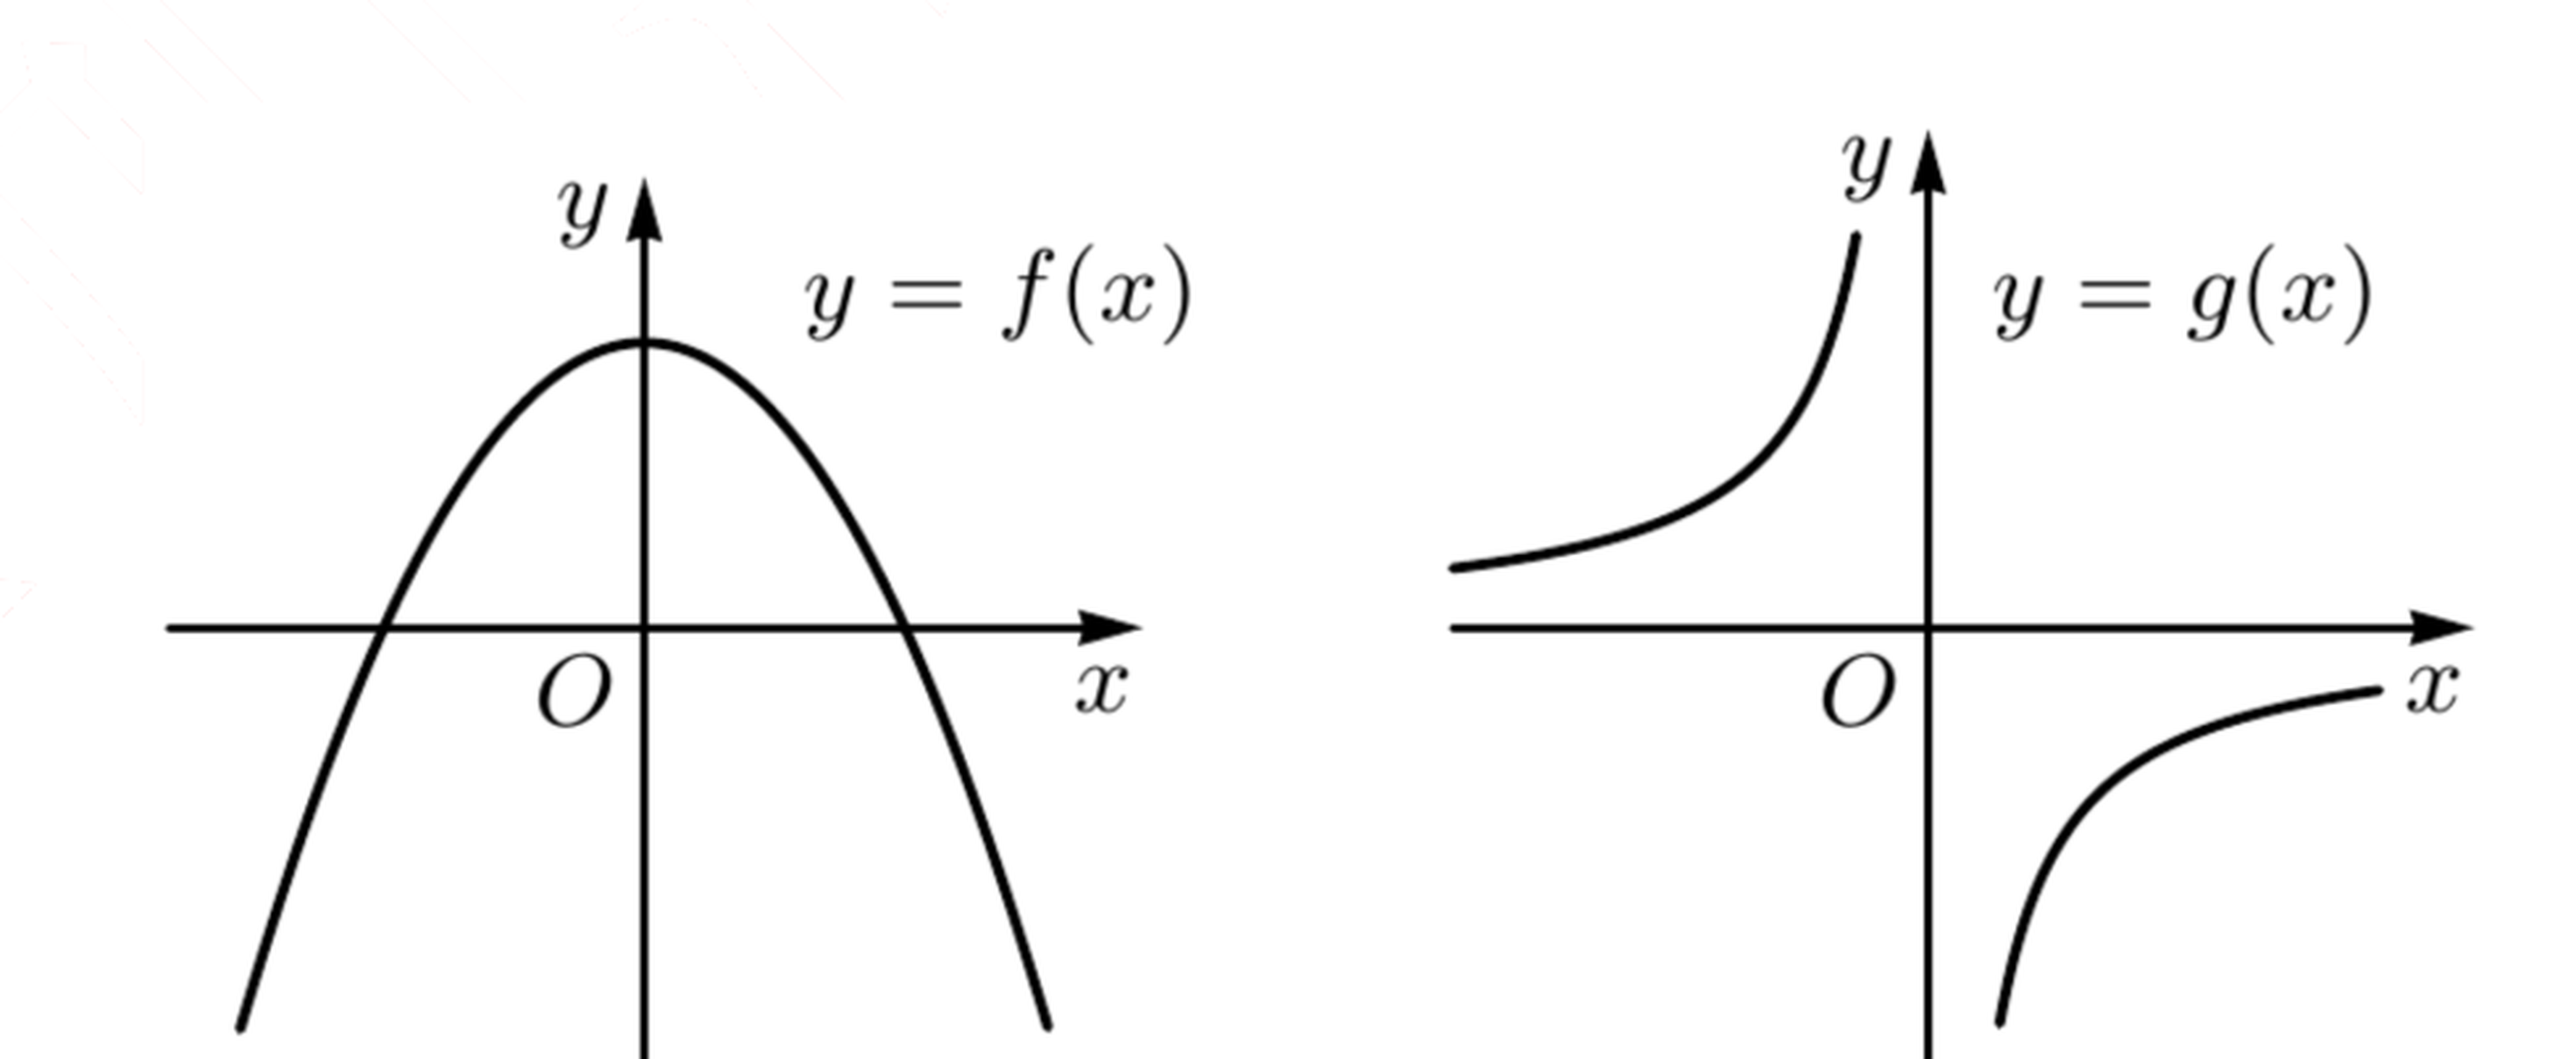
\includegraphics[width=0.72\textwidth]{figures/gao134_q13_graphs.png}\\[0.6em]
% A/B/C/D 四幅函数图象选项取原卷 04 页截图去粉色水印，按原卷一行四幅排布合并为一张
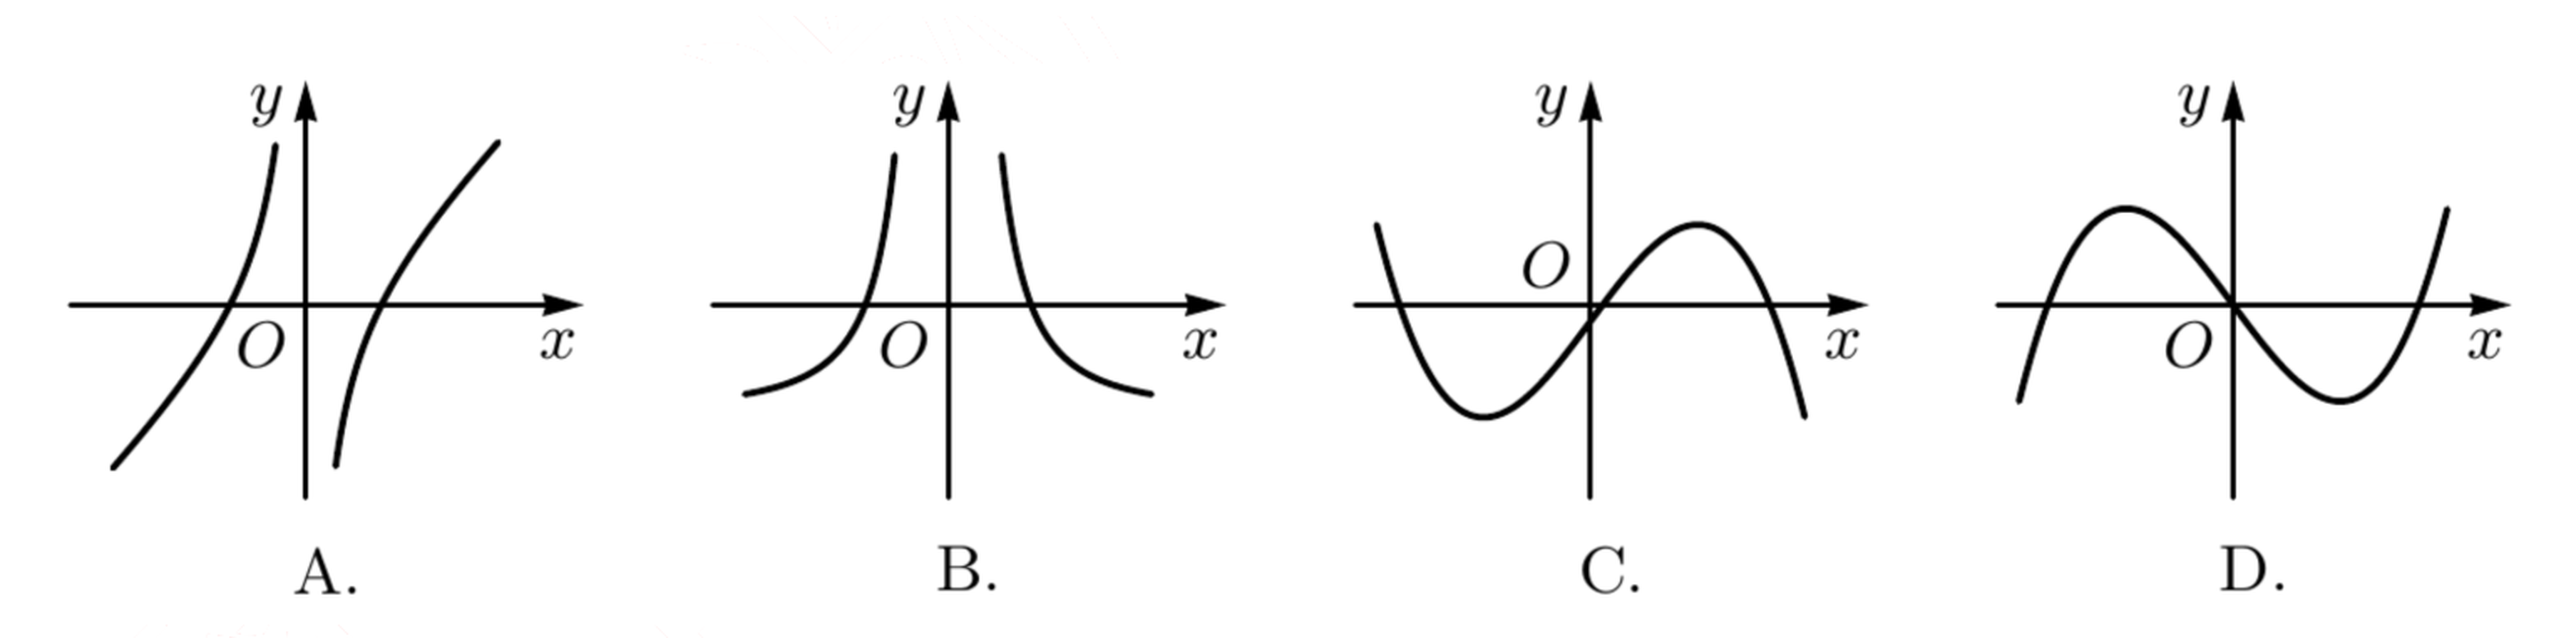
\includegraphics[width=0.90\textwidth]{figures/gao134_q13_options.png}
\end{center}

\ifanswer
\solbegin
\step{$f(x)$ 为偶函数，$g(x)$ 为奇函数，因此 $f(x)g(x)$ 为奇函数，排除 B.}
\step{又 $x=0$ 不在乘积函数的定义域内，其图象在 $y$ 轴上没有点，排除 C、D，}
\step{故选 $A$.}
\solend
\fi

\item 设全集为自然数集 $\N$，$E=\{x\mid x=2n,n\in\N\}$，$F=\{x\mid x=4n,n\in\N\}$，那么集合 $\N$ 可以表示成\mbox{（\quad）}

\keepwithprev
A. $E\cap F$\qquad\qquad B. $\overline{E}\cup F$\qquad\qquad C. $\overline{F}\cup E$\qquad\qquad D. $\overline{E}\cap\overline{F}$

\ifanswer
\solbegin
\step{$F\subseteq E$，所以 $\overline{F}\cup E=\N$，故选 $C$.}
\solend
\fi

\item 已知函数 $y=f(x)$，其中 $f(x)=x^2+bx$，则“$b<0$”是“$f(f(x))$ 的最小值与 $f(x)$ 的最小值相等”的\mbox{（\quad）}

\keepwithprev
A. 充分非必要条件\qquad\qquad B. 必要非充分条件

C. 充分必要条件\qquad\qquad D. 既非充分又非必要条件

\ifanswer
\solbegin
\step{$f(x)=\left(x+\dfrac b2\right)^2-\dfrac{b^2}4$，最小值为 $-\dfrac{b^2}4$，值域为 $\left[-\dfrac{b^2}4,+\infty\right)$.}
\step{当 $b<0$ 时，$-\dfrac b2>0\geqslant-\dfrac{b^2}4$，存在 $x$ 使 $f(x)=-\dfrac b2$，}
\step{从而 $f(f(x))$ 的最小值也为 $-\dfrac{b^2}4$，充分性成立.}
\step{当 $b=0$ 时，$f(x)=x^2$，$f(f(x))=x^4$，两者最小值均为 $0$，必要性不成立.}
\step{故选 $A$.}
\solend
\fi

\item 已知 $a,b,c\in\R$，若存在常数 $M>0$，使得 $a^2+b^2+c^2<M$，则称 $(a,b,c)$ 是有界数组. 对以下两个命题：

①若 $\lvert a^2+b+c\rvert+\lvert a^2+b-c\rvert\leqslant1$，则 $(a,b,c)$ 是有界数组；

②若 $\lvert a^2+b+c\rvert+\lvert a+b^2-c\rvert\leqslant1$，则 $(a,b,c)$ 是有界数组.% ②第二项为 \lvert a+b^2-c\rvert，与①刻意不同，照录

下列判断正确的是\mbox{（\quad）}

\keepwithprev
A. ①和②均为真命题\qquad\qquad B. ①和②均为假命题

C. ①为真命题，②为假命题\qquad D. ①为假命题，②为真命题

\ifanswer
\solbegin
\step{①取 $a=t,b=-t^2,c=0$，条件左端为 $0$，而 $a^2+b^2+c^2=t^2+t^4$ 可任意大，}
\step{故①为假命题.}
\step{②由条件，$a^2+a+b^2+b\leqslant\lvert a^2+b+c\rvert+\lvert a+b^2-c\rvert\leqslant1$.}
\step{由 $(a+1)^2+(b+1)^2\geqslant0$，得 $a^2+b^2\leqslant2(a^2+a+b^2+b)+2\leqslant4$.}
\step{又 $\lvert c\rvert\leqslant\lvert a^2+b+c\rvert+a^2+\lvert b\rvert\leqslant1+4+2=7$，故 $a^2+b^2+c^2\leqslant53<54$，}
\step{可取 $M=54$，故②为真命题.}
\step{故选 $D$.}
\solend
\fi

\end{enumerate}

\bigsec{三、解答题}

\begin{enumerate}
\setcounter{enumi}{16}

\item 已知不等式 $x^2-ax-b<0$ 的解集为 $A$，不等式 $\dfrac{3-2x}{x-1}<0$ 的解集为 $B$.

(1) 若 $a=5$，$b=-6$，求 $A\cap\overline{B}$；

(2) 若 $b=2a^2$，且 $A\cup B=B$，求实数 $a$ 的取值范围.

\ifanswer
\solbegin
\step{(1) 不等式 $\dfrac{3-2x}{x-1}<0$ 等价于 $x<1$ 或 $x>\dfrac32$，}
\step{所以 $B=(-\infty,1)\cup\left(\dfrac32,+\infty\right)$，$\overline{B}=\left[1,\dfrac32\right]$，}
\step{由 $x^2-5x+6=(x-2)(x-3)<0$，得 $A=(2,3)$，因此 $A\cap\overline{B}=\varnothing$.}
\step{(2) $A\cup B=B\Leftrightarrow A\subseteq B$，且 $x^2-ax-2a^2=(x-2a)(x+a)$，}
\step{当 $a=0$ 时，$A=\varnothing$，满足条件.}
\step{当 $a>0$ 时，$A=(-a,2a)$，$-a<0<1$，$A\subseteq B\Leftrightarrow2a\leqslant1$，得 $0<a\leqslant\dfrac12$.}
\step{当 $a<0$ 时，$A=(2a,-a)$，$2a<0<1$，$A\subseteq B\Leftrightarrow-a\leqslant1$，}
\step{得 $-1\leqslant a<0$.}
\step{因此 $a$ 的取值范围为 $\left[-1,\dfrac12\right]$.}
\solend
\fi

\item 为了在夏季降温和冬季供暖时减少能源损耗，房屋的屋顶和外墙需要建造隔热层. 某幢建筑物要建造可使用 $30$ 年的隔热层，每厘米厚的隔热层建造成本为 $9$ 万元. 该建筑物每年的能源消耗费用 $C$（万元）与隔热层厚度 $x$（cm）满足如下关系式：$C=\dfrac{k}{3x+5}$（$0\leqslant x\leqslant10$）. 若不建隔热层，每年能源消耗费用为 $8$ 万元. 设 $y$（万元）为隔热层建造费用与 $30$ 年的能源消耗费用之和.

(1) 求 $k$ 的值及 $y$ 的表达式；

(2) 隔热层修建多厚时，总费用 $y$ 最小？并求最小值.

\ifanswer
\solbegin
\step{(1) 不建隔热层时 $x=0$，$C=8$，所以 $\dfrac k5=8$，得 $k=40$.}
\step{隔热层建造费用为 $9x$ 万元，$30$ 年的能源消耗费用为 $30\times\dfrac{40}{3x+5}$ 万元.}
\step{因此 $y=9x+\dfrac{1200}{3x+5}$，$0\leqslant x\leqslant10$.}
\step{(2) 令 $t=3x+5$，则 $5\leqslant t\leqslant35$，且 $y=3t+\dfrac{1200}{t}-15$，}
\step{因为 $t>0$，由基本不等式得 $y\geqslant2\sqrt{3t\cdot\dfrac{1200}{t}}-15=105$，}
\step{当且仅当 $3t=\dfrac{1200}{t}$，即 $t=20$时取等号，此时 $x=5\in[0,10]$，}% 原卷"20"与"时"之间未留空，照录
\step{所以隔热层厚度为 $5$ cm 时，总费用最小，最小值为 $105$ 万元.}
\solend
\fi

\item 已知 $f(x)=ax^2+\dfrac1x$，其中 $a$ 为常数.

(1) 若 $a\in(1,3)$，判断函数 $y=f(x)$ 在 $[1,2]$ 上的单调性，并用定义证明；

(2) 求函数 $y=f(x)-x-\dfrac1x$ 在 $[1,2]$ 上的最大值 $g(a)$.

\ifanswer
\solbegin
\step{(1) 任取 $x_1,x_2\in[1,2]$，且 $x_1<x_2$，}
\step{则 $f(x_2)-f(x_1)=(x_2-x_1)\left[a(x_1+x_2)-\dfrac1{x_1x_2}\right]$，}
\step{由 $a>1$，$x_1+x_2\geqslant2$，$x_1x_2\geqslant1$，得 $a(x_1+x_2)-\dfrac1{x_1x_2}>2-1>0$，}
\step{因此 $f(x_2)>f(x_1)$，$f(x)$ 在 $[1,2]$ 上为严格增函数.}
\step{(2) 令 $h(x)=f(x)-x-\dfrac1x=ax^2-x$，其中 $x\in[1,2]$.}
\step{若 $a=0$，则 $h(x)=-x$，所以 $h(x)_{max}=h(1)=-1$；}
\step{若 $a<0$，二次函数的图象的对称轴为 $x=\dfrac1{2a}<0$，}
\step{所以 $y=h(x)$ 在 $[1,2]$ 上是严格减函数，所以 $h(x)_{max}=h(1)=a-1$；}
\step{若 $a>0$ 且 $\dfrac1{2a}>\dfrac32$，即 $0<a<\dfrac13$ 时，$h(x)_{max}=h(1)=a-1$.}
\step{若 $a>0$ 且 $\dfrac1{2a}\leqslant\dfrac32$，即 $a\geqslant\dfrac13$ 时，$h(x)_{max}=h(2)=4a-2$.}
\step{综上所述，$g(a)=\begin{cases}a-1,a<\dfrac13\\4a-2,a\geqslant\dfrac13\end{cases}$.}
\solend
\fi

\item 已知 $f(x)=\dfrac{ax^2+1}{bx+c}$（$a,b,c\in\Z$）.

(1) 若函数 $y=f(x)$ 是奇函数，且 $f(1)=2$，$f(2)<3$，求 $a,b,c$ 的值；

(2) 若函数 $y=f(x)$ 是偶函数，且 $ac<0$，$f(2a^2+a+1)<f(-3a^2+2a-1)$，求 $a$ 的值；

(3) 若 $b=a+c^2$，且满足不等式 $\lvert f(x)\rvert\geqslant1$ 的 $x$ 的最大值为 $0$，求 $c$ 的值.

\ifanswer
\solbegin
\step{(1) 由 $f(-x)=-f(x)$，交叉相乘得 $2c(ax^2+1)=0$ 恒成立，}
\step{因此 $c=0$，$b\neq0$.}
\step{由 $f(1)=2$，得 $a+1=2b$，}
\step{于是 $f(2)=\dfrac{4a+1}{2b}=4-\dfrac3{2b}<3\Leftrightarrow0<b<\dfrac32$，}
\step{因为 $b\in\Z$，所以 $b=1$，进而 $a=1$，$c=0$.}
\step{(2) 由 $f(-x)=f(x)$，交叉相乘得 $2bx(ax^2+1)=0$ 恒成立，因此 $b=0$.}
\step{此时 $f(x)=\dfrac ac x^2+\dfrac1c$，且 $\dfrac ac<0$.}
\step{设 $u=2a^2+a+1$，$v=-3a^2+2a-1$.}
\step{方程 $2a^2+a+1=0$ 与 $3a^2-2a+1=0$ 的判别式分别为 $-7$ 与 $-8$，}
\step{都小于 $0$，所以 $u>0$，$v<0$.}
\step{于是 $f(u)<f(v)\Leftrightarrow u^2>v^2\Leftrightarrow u>-v\Leftrightarrow-a^2+3a>0\Leftrightarrow0<a<3$，}
\step{因为 $a\in\Z$，所以 $a=1$ 或 $a=2$.}
\step{(3) 因为解集的最大值为 $0$，所以 $f(0)$ 有定义且 $\lvert f(0)\rvert\geqslant1$，}
\step{即 $c\neq0$，$\left\lvert\dfrac1c\right\rvert\geqslant1$，结合 $c\in\Z$，得 $c=\pm1$，从而 $b=a+1$.}
\step{当 $x=2$ 时，分母 $2a+2+c$ 为奇数，必不为 $0$；}
\step{又因为 $2>0$，必须有 $\lvert f(2)\rvert<1\Leftrightarrow\lvert4a+1\rvert<\lvert2a+2+c\rvert$，}
\step{若 $c=-1$，则 $(4a+1)^2<(2a+1)^2\Leftrightarrow4a(3a+1)<0\Leftrightarrow-\dfrac13<a<0$，}
\step{不存在满足条件的整数 $a$.}
\step{若 $c=1$，则 $(4a+1)^2<(2a+3)^2\Leftrightarrow4(3a+2)(a-1)<0\Leftrightarrow-\dfrac23<a<1$，}
\step{所以 $a=0$，$b=1$，此时 $f(x)=\dfrac1{x+1}$，}
\step{且 $\lvert f(x)\rvert\geqslant1\Leftrightarrow0<\lvert x+1\rvert\leqslant1\Leftrightarrow x\in[-2,-1)\cup(-1,0]$，}
\step{解集的最大值确为 $0$，因此 $c=1$.}
\solend
\fi

\item 已知函数 $y=f(x)$ 的定义域为 $\R$，且当 $x>0$ 时，$f(x)=\dfrac1{x+1}$. 对任意 $x_0\in\R$，定义集合 $D(x_0)=\{d\mid f(x_0+d)>f(x_0)\}$.

(1) 若当 $x\leqslant0$ 时，$f(x)=-2x+1$，求函数 $y=f(x)$ 的值域；

(2) 若 $y=f(x)$ 是偶函数，且 $f(0)=1$，求证：$D(-2)=\{-d\mid d\in D(2)\}$；

(3) 若 $y=f(x)$ 是奇函数，且 $x_1x_2\neq0$，求证：“$f(x_1)\leqslant f(x_2)$”的充要条件是\!\mbox{“$D(x_2)\subseteq D(x_1)$”}.

\ifanswer
\solbegin
\step{(1) 当 $x>0$ 时，$0<f(x)<1$；当 $x\leqslant0$ 时，$f(x)=-2x+1\geqslant1$.}
\step{函数的值域为 $(0,1)\cup[1,+\infty)=(0,+\infty)$.}
\step{(2) 由 $f(x)$ 是偶函数及 $f(0)=1$，得 $f(x)=\dfrac1{1+\lvert x\rvert}$，且 $f(2)=f(-2)=\dfrac13$.}
\stepm{法一：}{$D(2)=\left\{d\mid\dfrac1{1+\lvert2+d\rvert}>\dfrac13\right\}=\{d\mid\lvert2+d\rvert<2\}=(-4,0)$，}
\step{$D(-2)=\left\{d\mid\dfrac1{1+\lvert-2+d\rvert}>\dfrac13\right\}=\{d\mid\lvert-2+d\rvert<2\}=(0,4)$，}
\step{因此 $\{-d\mid d\in D(2)\}=(0,4)=D(-2)$.}
\stepm{法二：}{任取 $d\in D(-2)$，由定义得 $f(-2+d)>f(-2)$.}
\step{因为 $y=f(x)$ 是偶函数，所以对任意的实数 $x$，有 $f(-x)=f(x)$，}
\step{因此 $f(-2+d)=f(-(-2+d))=f(2-d)$，且 $f(-2)=f(2)$.}
\step{所以不等式 $f(-2+d)>f(-2)$ 等价于 $f(2-d)>f(2)$，}
\step{这恰好是 $-d\in D(2)$ 的定义，}
\step{所以 $d\in D(-2)\Leftrightarrow-d\in D(2)$，故 $D(-2)=\{-d\mid d\in D(2)\}$.}
\step{(3) 由 $f(x)$ 是奇函数，得 $f(0)=0$；}
\step{当 $x<0$ 时，$f(x)=-f(-x)=-\dfrac1{1-x}=\dfrac1{x-1}$；}
\step{所以 $f(x)=\begin{cases}\dfrac1{x-1},&x<0\\0,&x=0;\\\dfrac1{x+1},&x>0\end{cases}$}
% 2026-11-15 回原图订正：原卷 11 页此 cases 块末无句点，本稿初转顺手补了西文句点，今删去（Q19 08 页同类块末有句点，照录保留）。
\step{当 $x_0<0$ 时，$D(x_0)=\{d\mid f(x_0+d)>f(x_0)\}=(-\infty,0)\cup[-x_0,+\infty)$，}
\step{当 $x_0=0$ 时，$D(0)=\{d\mid f(0+d)>f(0)\}=(0,+\infty)$，}
\step{当 $x_0>0$ 时，$D(x_0)=\{d\mid f(x_0+d)>f(x_0)\}=(-x_0,0)$.}
\stepm{先证明必要性.}{若 $f(x_1)\leqslant f(x_2)$，仅需讨论三类情形：}
\step{若 $x_2\leqslant x_1<0$，}
\step{则 $D(x_1)=(-\infty,0)\cup[-x_1,+\infty),D(x_2)=(-\infty,0)\cup[-x_2,+\infty)$，}
\step{故 $D(x_2)\subseteq D(x_1)$；}
\step{若 $0<x_2\leqslant x_1$，则 $D(x_1)=(-x_1,0),D(x_2)=(-x_2,0)$，}
\step{故 $D(x_2)\subseteq D(x_1)$；}
\step{若 $x_1<0<x_2$，则 $D(x_1)=(-\infty,0)\cup[-x_1,+\infty),D(x_2)=(-x_2,0)$，}
\step{故 $D(x_2)\subseteq D(x_1)$.}
\stepm{再证明充分性.}{若 $D(x_2)\subseteq D(x_1)$，}
\step{若 $x_1<0,x_2<0$，}
\step{则 $D(x_1)=(-\infty,0)\cup[-x_1,+\infty),D(x_2)=(-\infty,0)\cup[-x_2,+\infty)$，}
\step{由 $D(x_2)\subseteq D(x_1)$ 得 $x_2\leqslant x_1$，}
\step{又 $y=f(x)$ 在 $(-\infty,0)$ 上是严格减函数，所以 $f(x_1)\leqslant f(x_2)$；}
\step{若 $x_1>0,x_2>0$，则 $D(x_1)=(-x_1,0),D(x_2)=(-x_2,0)$，}
\step{由 $D(x_2)\subseteq D(x_1)$ 得 $x_2\leqslant x_1$，}
\step{又 $y=f(x)$ 在 $(0,+\infty)$ 上是严格减函数，所以 $f(x_1)\leqslant f(x_2)$；}
\step{若 $x_1<0,x_2>0$，则 $f(x_1)<0<f(x_2)$，结论成立；}
\step{若 $x_1>0,x_2<0$，此时 $D(x_1)=(-x_1,0)$ 中只有负数，}
\step{而 $D(x_2)=(-\infty,0)\cup[-x_2,+\infty)$ 中有正数，$D(x_2)\subseteq D(x_1)$ 不成立.}
\step{综上，“$f(x_1)\leqslant f(x_2)$”的充要条件是“$D(x_2)\subseteq D(x_1)$”.}
\solend
\fi

\end{enumerate}

\end{document}
"
%
% ① 原始材料：微信公众号"魔都数学加油站"文章，作者破晓，2026-11-15 18:04 发布；
% 连载"27学年高一134"，原文标题"27学年高一134——2026-2027年上海市华师大二附中高一上期中"；
% 原文链接：https://mp.weixin.qq.com/s/bQlkmlGdCtAlytY331vf3g。
% 正文为 13 张 PNG 页（01、04、06、08、09、10、11、12、13 为 2560x3620；
% 02、03、05、07 为 4762x6735，同一篇各页分辨率不同，逐页按各自分辨率裁图核对），
% 题目下印有【解析】，为讲评版。题目、解析均据原图转录；卷面粉红色水印
% "魔都数学加油站"及公众号页脚未录入。
% 全卷 2 幅插图，均在第 04 页：第 13 题题干 y=f(x)、y=g(x) 两幅函数图象合并裁为
% figures/gao134_q13_graphs.png，第 13 题 A/B/C/D 四幅函数图象选项合并裁为
% figures/gao134_q13_options.png；两图均取原卷 04 页截图 3× LANCZOS 放大、
% 白化粉色水印（只白化浅粉色 R>175 且 G>140 且 B>140 的像素，保留红色标签）。
% 注意：本卷 Q13 四幅选项在原卷排为"一行四幅"（1×4），并非 高一132 第 14 题
% 的 2×2 排布，本稿按原卷 1×4 合并裁为一张，不重排、不用 TikZ 重绘。
%
% 卷首标题：原卷印作"2026-2027 年华师大二附中高一上期中"（公众号标题中的"上海市"
% 卷面标题行没有，本稿照卷面），年份区间按全稿惯例排 en dash；原卷未印副标题，
% 本卷为期中卷、跨集合与常用逻辑用语／不等式／函数三章，按题目内容标为
% "集合与常用逻辑用语、不等式、函数"（与 125／126／128／129／131／132／133 同期中卷口径相同）：
% 集合与逻辑见 Q6、Q10、Q14、Q16、Q17、Q21，不等式见 Q3、Q7、Q9、Q11、Q15、Q18、Q19，
% 函数（函数性质、二分法、奇偶性、基本不等式应用）见 Q4、Q5、Q8、Q12、Q13、Q20。
%
% 题号体例：本卷共 19 题——一、填空题 3—12（10 题）、二、选择题 13—16（4 题）、
% 三、解答题 17—21（5 题）。三节分别 \setcounter{enumi}{2}／{12}／{16}。
% 第 13 页仅为 Q21 (3) 解析续尾，全卷无「四、附加题」。
%
% ② 与原卷的排版差异：
%   ① 原文从第 3 题起，本稿保留原题号（见上"题号体例"）；
%   ② 原卷每题下直接印【解析】，本稿按全稿惯例置于答案版；第 13—16 题答案均在
%      解析末句"故选 …"，题干括号内留空、不另提 \ans{}（四题均无独立答案段）；
%      全卷无只印括号内答案、无解析的选择题；
%   ③ 原卷未印副标题，本稿按"知识模块"口径补出；
%   ④ 原卷填空横线按全稿惯例排为 \blankline[4.4em]；选择题括号排 \mbox{（\quad）}、
%      每个选项段前按惯例加 \keepwithprev（Q13 四选项为图，守卫前行为 \begin{center}；
%      Q15、Q16 四选项分两行排，\keepwithprev 只加在 A. 行前）；解答题不留作答区、
%      不加 \anspace（原卷为讲评版，与 129／131／132／133 同）；
%   ⑤ 原卷数集印黑板粗体（Q7／Q11／Q12／Q16／Q21 的 R、Q14／Q20 的 N、Q20 的 Z），
%      按全稿惯例统一排 \R／\N／\Z；绝对值排 \lvert…\rvert，集合描述竖线排 \mid；不等号按全稿惯例排
%      \leqslant／\geqslant；补集照原卷上划线排 \overline{B}、\overline{E}、\overline{F}；
%   ⑥ 子题标号 (1)(2)(3) 与括注原卷均用半角括号，照录（与 131／132／133 同）；
%      圈数字 ①② 照录；原卷 Q21 (2) 解析"法一：""法二："与 Q21 (3) 解析
%      "先证明必要性.""再证明充分性."四处标签印红色加粗，按 高一53／108／133 成例排
%      \stepm{法一：}／\stepm{法二：}／\stepm{先证明必要性.}／\stepm{再证明充分性.}
%      （加粗着色、不引入红色，不动 common.sty）；Q8 解析"第 1 步：""第 2 步：""
%      "第 3 步："原卷印黑色常规宋体（非红非粗），照录为普通 \step 行内文字；
%   ⑦ 数学式内半角逗号照录（如 Q6 $A=\{0,1,2,3\}$、Q14 $x=2n,n\in\N$、
%      Q16 $a,b,c\in\R$ 与 $a=t,b=-t^2,c=0$、Q19 $x_1,x_2\in[1,2]$、
%      Q20 $a,b,c\in\Z$、Q21 $x_1<0,x_2<0$ 与 $D(x_1)=(-x_1,0),D(x_2)=(-x_2,0)$）；
%      原卷行末全角句点按全稿惯例从宽排西文句点；cases 块末的句点逐处照录：
%      Q19 解析（08 页）块末原卷有句点照录、Q21 (3) 解析（11 页）块末原卷无句点不补，
%      两处原卷自身不统一（2026-11-15 回原图核对，本稿初转曾顺手补句点，已删去）；
%   ⑧ 原卷 Q8 解析跨 01—02 页、Q10 解析跨 02—03 页、Q12 解析跨 03—04 页、
%      Q16 解析跨 05—06 页、Q17 解析跨 06—07 页、Q20 解析跨 08—10 页、
%      Q21 解析跨 10—13 页，本稿按题合并连续排版；末页第 13 页为
%      Q21 (3) 解析续尾与"综上"一句，按实际印刷行单列；
%   ⑨ 题干中的中文弯引号按原卷照录（Q10 研究问题、Q15 条件、Q21 (3) 充要条件），
%      注释内一律 ASCII 引号。
%
% 判别式字形：全卷仅 Q9 解析末行出现一处判别式记号
%   "两值均满足 $\Delta=p^2-4p=18\mp12\sqrt2>0$"，逐处放大核对，原卷印高三角
%   $\Delta$（等腰、高，实测高宽比约 1.14），照录 \Delta；卷内无扁三角 \triangle，
%   与 高一132 同题排 $\triangle$、高一133 部分判别式排 $\triangle$ 均不同。
%
% 子集符号：Q6 题干 $C\subseteq A$、$C\subseteq B$ 与解析 $C\subseteq A\cap B$、
%   Q14 解析 $F\subseteq E$、Q17 解析 $A\subseteq B$、Q21 题干与解析各处的
%   $D(x_2)\subseteq D(x_1)$，全部印带下划线的 $\subseteq$，逐处放大核对，
%   照录 \subseteq；全卷未出现单线 \subset。
%
% 原卷存疑照录（均照录未改，正文对应处另有 % 注）：
%   第 6 题题干集合 $A=\{0,1,2,3\}$ 三个逗号后不留空，紧邻的 $B=\{0,2,4,5\}$
%      三个逗号后却留空，同卷同一行两集合排字不一，照录其逗号均为半角；
%   第 16 题命题②作 $\lvert a^2+b+c\rvert+\lvert a+b^2-c\rvert\leqslant1$，
%      与命题①第二项 $\lvert a^2+b-c\rvert$ 不同（①无 $b$ 的平方、②有），
%      两命题刻意不同，照录；解析"②由条件，$a^2+a+b^2+b\leqslant\cdots$"
%      由两项相加直接得到，照录；
%   第 18 题 (2) 解析"即 $t=20$时取等号"中"20"与"时"之间原卷未留空，照录；
%   第 19 题解析 $h(x)_{max}$ 的"max"下标三处字形不一（斜体／正体混排），照录；
%   第 20 题 (1)(2) 解析"由 $f(-x)=-f(x)$，交叉相乘得……"与"由 $f(-x)=f(x)$，
%      交叉相乘得……"两处措辞照录；
%   第 21 题 (2) 原卷并存"法一"（集合计算）与"法二"（定义推证）两套证明，照录不删。
%
% 行数复核：逐题数 \step/\stepm 条数，合计 134 条（Q3：2；Q4：1；Q5：1；Q6：1；
% Q7：2；Q8：4；Q9：3；Q10：4；Q11：5；Q12：8；Q13：3；Q14：1；Q15：5；
% Q16：7；Q17：9；Q18：7；Q19：11；Q20：22；Q21：38），与原卷印刷行逐题相等
% （cases 块作一个印刷行计）。第 13—16 题答案在解析末句，括号内留空、不另提 \ans{}；
% 第 21 题四条 \stepm 计入 38 条内。
%
\documentclass[a4paper,11pt]{article}
\usepackage{common}

\begin{document}

\examtitlest[3]{2026--2027 年华师大二附中高一上期中}{集合与常用逻辑用语、不等式、函数}

\bigsec{一、填空题}

\begin{enumerate}
\setcounter{enumi}{2}

\item 不等式 $\lvert 2x+1\rvert\geqslant3$ 的解集为\blankline[4.4em].

\ifanswer
\solbegin
\step{$\lvert 2x+1\rvert\geqslant3\Leftrightarrow 2x+1\leqslant-3$ 或 $2x+1\geqslant3\Leftrightarrow x\leqslant-2$ 或 $x\geqslant1$，}
\step{故解集为 $(-\infty,-2]\cup[1,+\infty)$.}
\solend
\fi

\item 函数 $y=\sqrt{x+1}+\dfrac1x$ 的定义域为\blankline[4.4em].

\ifanswer
\solbegin
\step{$x+1\geqslant0$ 且 $x\neq0$，得定义域为 $[-1,0)\cup(0,+\infty)$.}
\solend
\fi

\item 已知等式 $3x^2-4x-2=a(x-1)^2+b(x-1)+c$ 恒成立，其中 $a$、$b$、$c$ 为常数，则 $a-b+c=$\blankline[4.4em].

\ifanswer
\solbegin
\step{令 $x=0$，得 $a-b+c=-2$.}
\solend
\fi

\item 已知集合 $A=\{0,1,2,3\}$，$B=\{0,2,4,5\}$，$C\subseteq A$，$C\subseteq B$，符合条件的集合 $C$ 有\blankline[4.4em]个.% 原卷 A 的逗号后不留空、B 的逗号后留空，排字不一，照录

\ifanswer
\solbegin
\step{$C\subseteq A\cap B=\{0,2\}$，所以符合条件的集合 $C$ 有 $2^2=4$ 个.}
\solend
\fi

\item 设 $a$、$b\in\R$，且 $a^2+4b^2=2$，则 $ab$ 的最大值为\blankline[4.4em].

\ifanswer
\solbegin
\step{$(a-2b)^2=a^2+4b^2-4ab=2-4ab\geqslant0$，得 $ab\leqslant\dfrac12$，}
\step{当且仅当 $a=2b=\pm1$ 时取等号，故 $ab$ 的最大值为 $\dfrac12$.}
\solend
\fi

\item 已知函数 $y=x(13-2x)^2-140$，用二分法求函数在区间 $(3,4)$ 上的零点时，第 3 步应计算 $x=$\blankline[4.4em]的函数值.

\ifanswer
\solbegin
\step{记 $f(x)=x(13-2x)^2-140$，则 $f(3)=7>0$，$f(4)=-40<0$.}
\step{第 1 步：$f\left(\dfrac72\right)=-14<0$，区间缩小为 $\left(3,\dfrac72\right)$.}
\step{第 2 步：$f\left(\dfrac{13}4\right)=-\dfrac{43}{16}<0$，区间缩小为 $\left(3,\dfrac{13}4\right)$.}
\step{第 3 步：应计算 $x=\dfrac{3+\frac{13}4}2=\dfrac{25}8$ 的函数值.}
\solend
\fi

\item 已知一元二次方程 $x^2+px+p=0$ 的两个实根分别为 $x_1$、$x_2$，且 $x_1^2x_2+x_2^2x_1=-18$，则 $p=$\blankline[4.4em].% 判别式 \Delta 高三角，逐处放大核对

\ifanswer
\solbegin
\step{由韦达定理，$x_1+x_2=-p$，$x_1x_2=p$，}
\step{则 $x_1^2x_2+x_2^2x_1=x_1x_2(x_1+x_2)=-p^2=-18\Rightarrow p=\pm3\sqrt2$，}
\step{两值均满足 $\Delta=p^2-4p=18\mp12\sqrt2>0$，故 $p=\pm3\sqrt2$.}
\solend
\fi

\item 研究问题：“已知关于 $x$ 的不等式 $ax^2-bx+c>0$ 的解集为 $(1,2)$，解关于 $x$ 的不等式 $cx^2-bx+a>0$”，有如下解法：

解：由 $ax^2-bx+c>0\Rightarrow a-b\left(\dfrac1x\right)+c\left(\dfrac1x\right)^2>0$，令 $y=\dfrac1x$，则 $y\in\left(\dfrac12,1\right)$，

所以不等式 $cx^2-bx+a>0$ 的解集为 $\left(\dfrac12,1\right)$.

参考上述解法，已知关于 $x$ 的不等式 $\dfrac{k}{x+a}+\dfrac{x+b}{x+c}<0$ 的解集为 $(-3,-1)\cup(2,4)$，则关于 $x$ 的不等式 $\dfrac{kx}{ax-1}+\dfrac{bx-1}{cx-1}<0$ 的解集为\blankline[4.4em].

\ifanswer
\solbegin
\step{当 $x=0$ 时，所求不等式左端为 $1$，不满足不等式.}
\step{当 $x\neq0$ 时，两个分式的分子、分母同除以 $x$，得 $\dfrac{k}{a-\frac1x}+\dfrac{b-\frac1x}{c-\frac1x}<0$.}
\step{令 $t=-\dfrac1x$，则所求不等式化为 $\dfrac{k}{t+a}+\dfrac{t+b}{t+c}<0$，即 $-\dfrac1x\in(-3,-1)\cup(2,4)$，}
\step{解得 $x\in\left(-\dfrac12,-\dfrac14\right)\cup\left(\dfrac13,1\right)$.}
\solend
\fi

\item 已知 $a\in(0,+\infty)$，若对任意的 $x\in(0,+\infty)$，均有 $\lvert x^2-a\rvert+\lvert x+b\rvert=\lvert x^2+x-a+b\rvert$，则 $a^2-b^2$ 的最小值为\blankline[4.4em].

\ifanswer
\solbegin
\step{原等式成立的充要条件是 $(x^2-a)(x+b)\geqslant0$.}
\step{当 $0<x<\sqrt a$ 时须有 $x+b\leqslant0$；当 $x>\sqrt a$ 时须有 $x+b\geqslant0$，因此 $b=-\sqrt a$.}
\step{此时 $(x^2-a)(x+b)=(x+\sqrt a)(x-\sqrt a)^2\geqslant0$，满足题意.}
\step{$a^2-b^2=a^2-a=\left(a-\dfrac12\right)^2-\dfrac14\geqslant-\dfrac14$，}
\step{当 $a=\dfrac12$，$b=-\dfrac{\sqrt2}2$ 时取等号，最小值为 $-\dfrac14$.}
\solend
\fi

\item 已知函数 $y=f(x)$ 在 $\R$ 上是严格增函数，当 $x\neq0$ 且 $f(x)\neq0$ 时，满足 $f(x)\cdot f\left[\dfrac1{f(x)}+\dfrac1x\right]=1$，则 $f(1)=$\blankline[4.4em].

\ifanswer
\solbegin
\step{当 $xf(x)>0$ 时，记 $t=\dfrac1{f(x)}+\dfrac1x\neq0$，则 $f(t)=\dfrac1{f(x)}\neq0$.}
\step{将 $t$ 代入题设，得 $f\left(f(x)+\dfrac1t\right)=f(x)$，严格增性给出 $f(x)+\dfrac1t=x$，}
\step{化简得 $f(x)^2+xf(x)-x^2=0$，由 $\dfrac{f(x)}x>0$ 得 $f(x)=\dfrac{\sqrt5-1}2x$.}
\step{设 $a=f(0)$，若 $a>0$，则 $f(a)>f(0)=a>0$；}
\step{若 $a<0$，则 $f(a)<f(0)=a<0$.}
\step{两种情形都有 $af(a)>0$ 且 $\dfrac{f(a)}a>1$，与上式 $\dfrac{f(a)}a=\dfrac{\sqrt5-1}2<1$ 矛盾，}
\step{因此 $f(0)=0$.}
\step{于是 $f(1)>0$，代入上式得 $f(1)=\dfrac{\sqrt5-1}2$.}
\solend
\fi

\end{enumerate}

% 第 13 题是"节标题 + 题干 + 两幅图 + 四幅选项图"约 15cm 的整块，
% 守卫只放在 \bigsec 之前；若再在 \item 之前放第二枚，会在标题已印出后才触发换页，
% 把题目推走、留下孤立节标题（切页审计 B 类）。高度须覆盖整块。
\needvspace{16cm}
\bigsec{二、选择题}

\begin{enumerate}
\setcounter{enumi}{12}

\item 已知函数 $y=f(x)$ 与 $y=g(x)$ 的图象如图所示，则函数 $y=f(x)\cdot g(x)$ 的图象可能是\mbox{（\quad）}

\keepwithprev
\begin{center}
% 题干 y=f(x)、y=g(x) 两幅函数图象取原卷 04 页截图去粉色水印，按原卷左右排布合并为一张
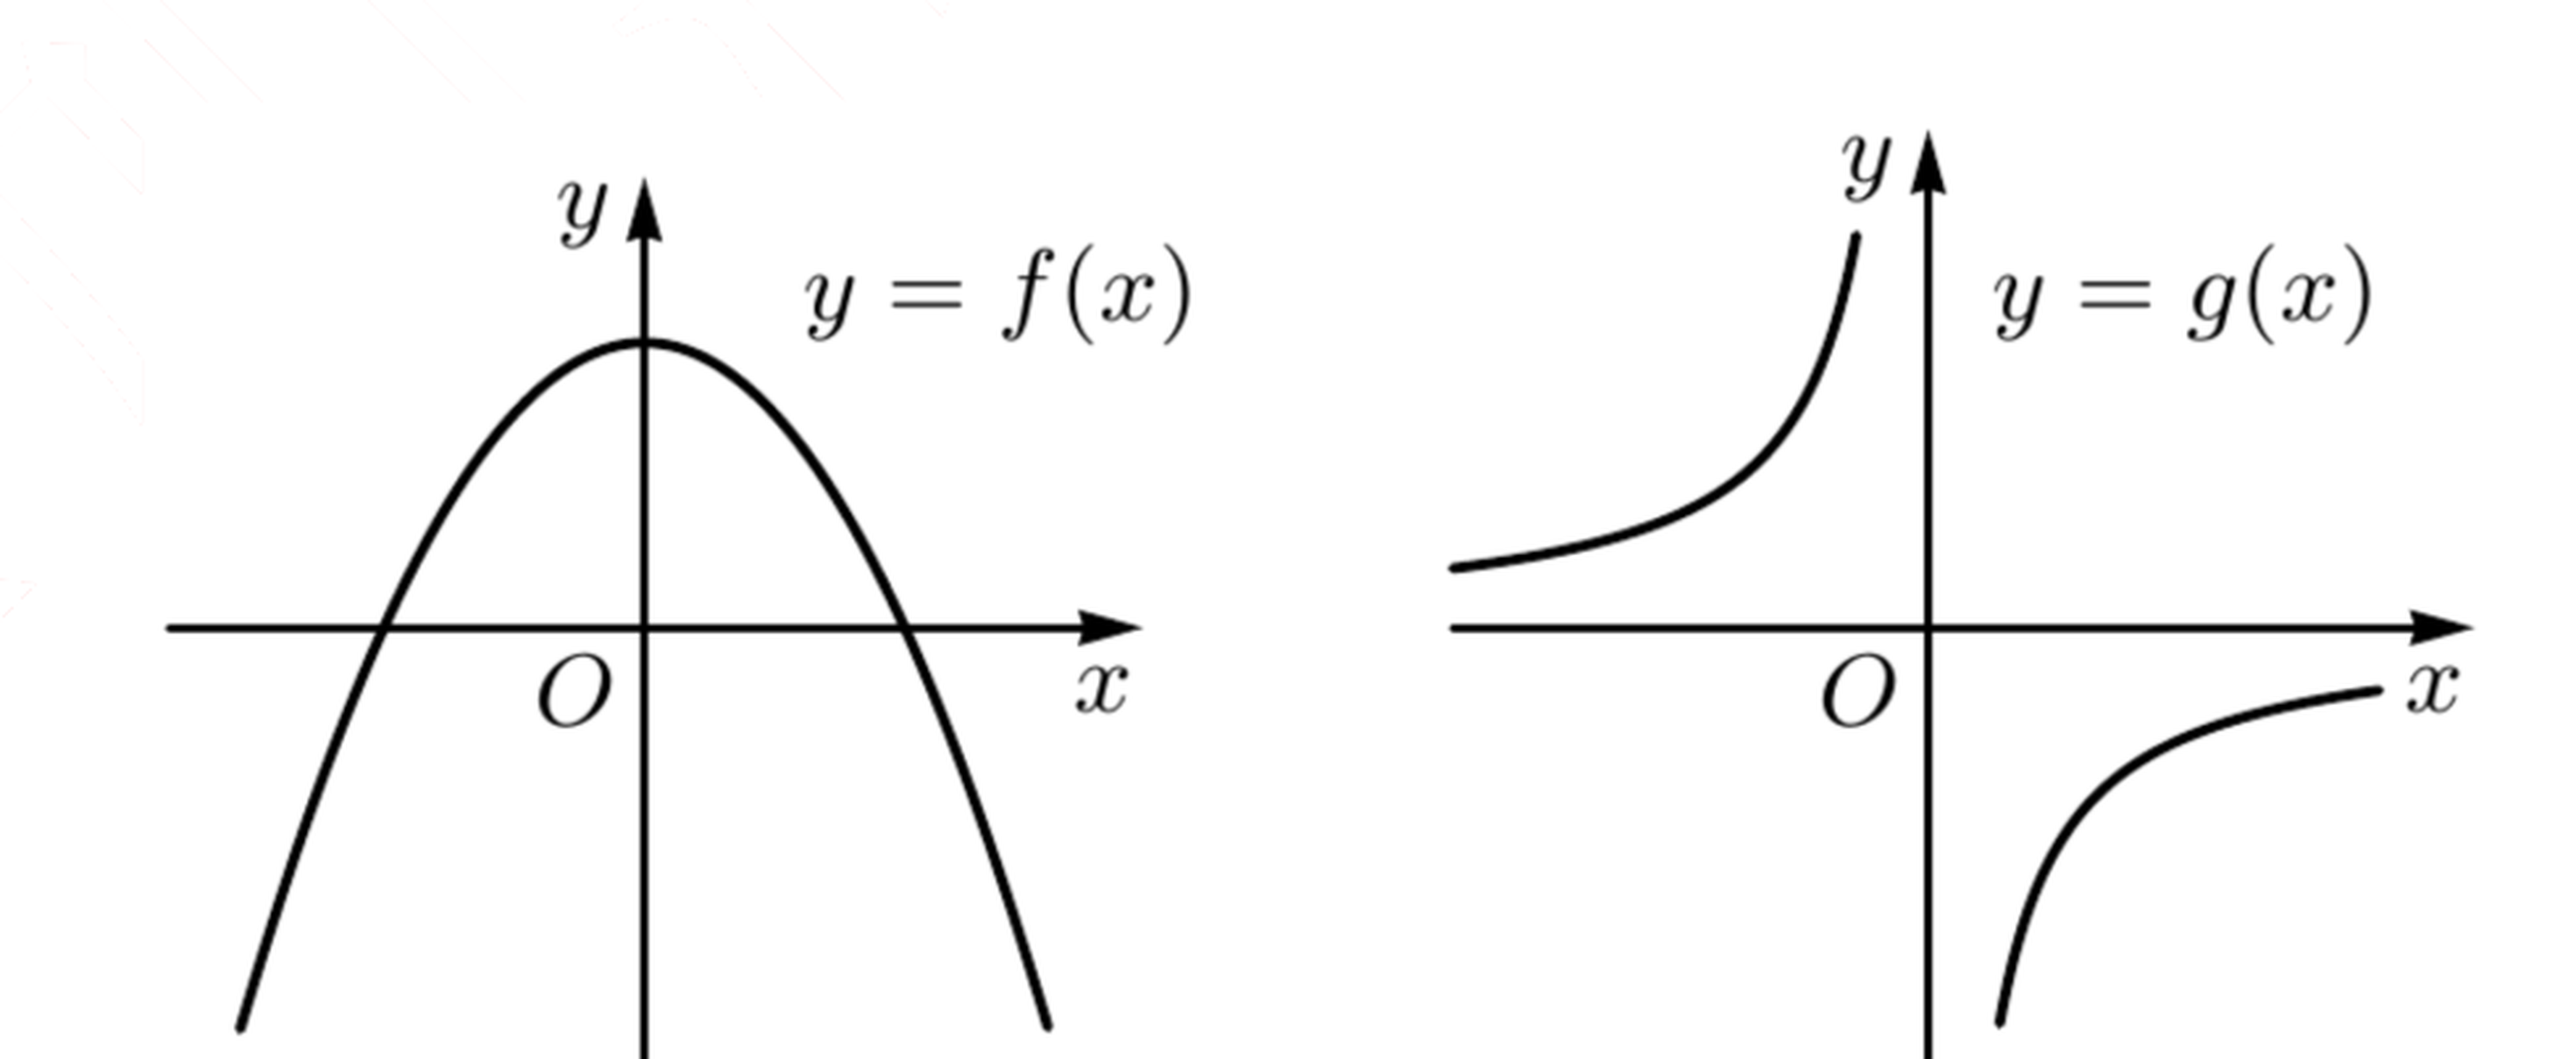
\includegraphics[width=0.72\textwidth]{figures/gao134_q13_graphs.png}\\[0.6em]
% A/B/C/D 四幅函数图象选项取原卷 04 页截图去粉色水印，按原卷一行四幅排布合并为一张
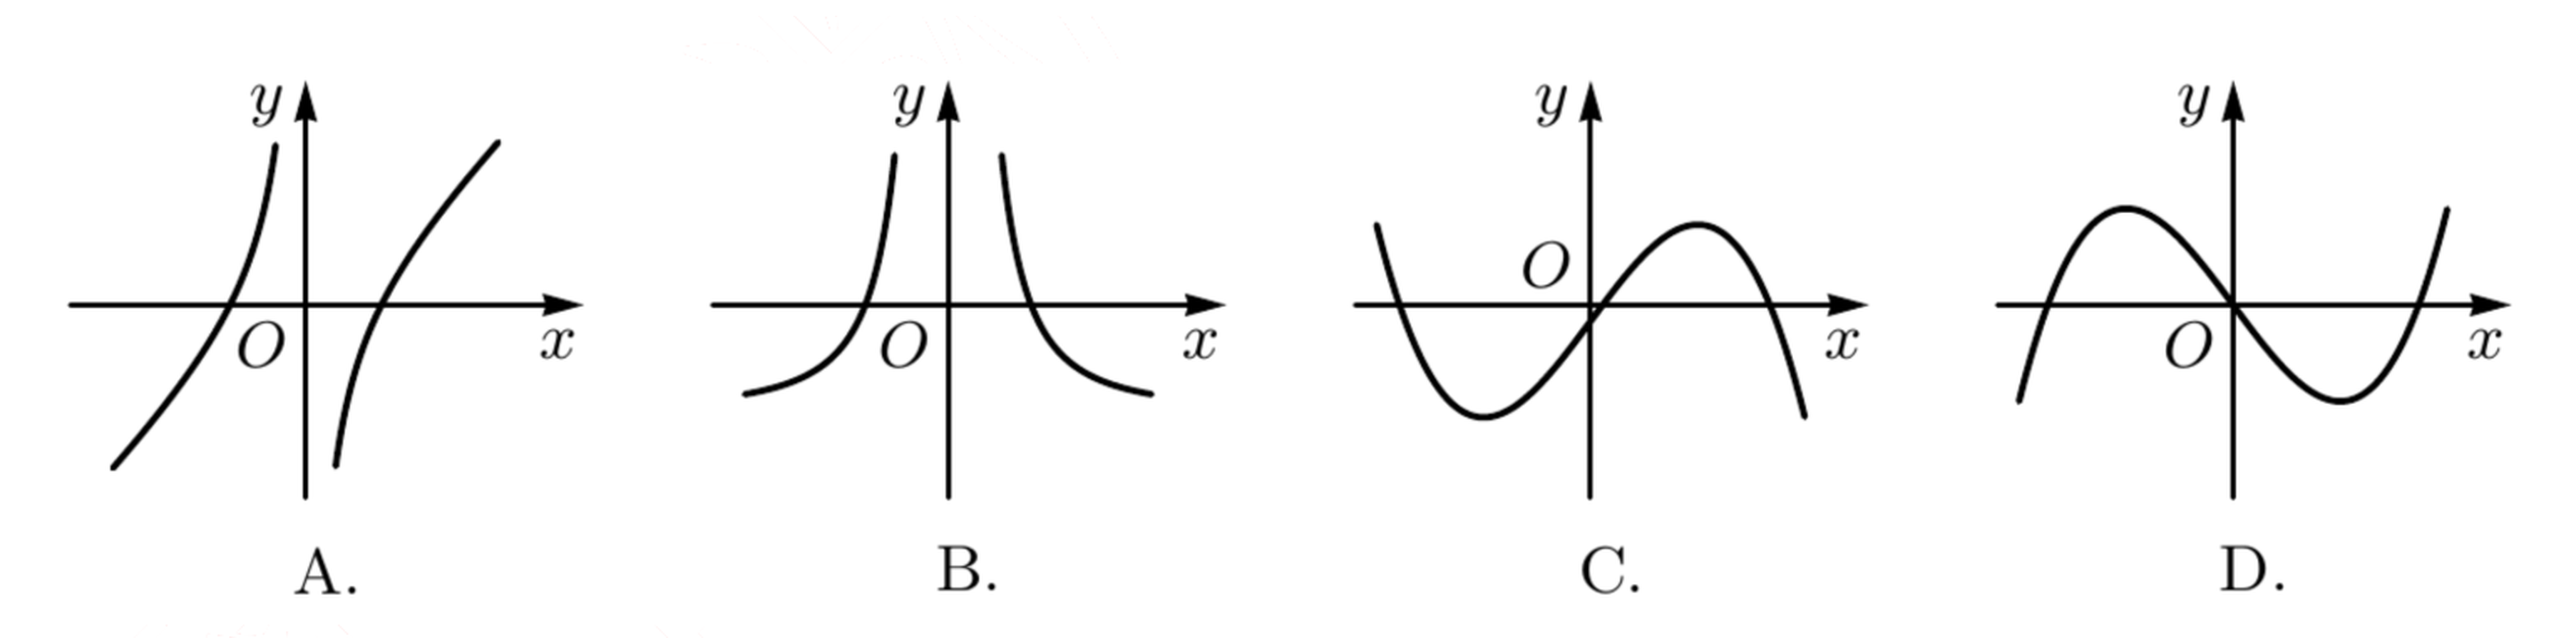
\includegraphics[width=0.90\textwidth]{figures/gao134_q13_options.png}
\end{center}

\ifanswer
\solbegin
\step{$f(x)$ 为偶函数，$g(x)$ 为奇函数，因此 $f(x)g(x)$ 为奇函数，排除 B.}
\step{又 $x=0$ 不在乘积函数的定义域内，其图象在 $y$ 轴上没有点，排除 C、D，}
\step{故选 $A$.}
\solend
\fi

\item 设全集为自然数集 $\N$，$E=\{x\mid x=2n,n\in\N\}$，$F=\{x\mid x=4n,n\in\N\}$，那么集合 $\N$ 可以表示成\mbox{（\quad）}

\keepwithprev
A. $E\cap F$\qquad\qquad B. $\overline{E}\cup F$\qquad\qquad C. $\overline{F}\cup E$\qquad\qquad D. $\overline{E}\cap\overline{F}$

\ifanswer
\solbegin
\step{$F\subseteq E$，所以 $\overline{F}\cup E=\N$，故选 $C$.}
\solend
\fi

\item 已知函数 $y=f(x)$，其中 $f(x)=x^2+bx$，则“$b<0$”是“$f(f(x))$ 的最小值与 $f(x)$ 的最小值相等”的\mbox{（\quad）}

\keepwithprev
A. 充分非必要条件\qquad\qquad B. 必要非充分条件

C. 充分必要条件\qquad\qquad D. 既非充分又非必要条件

\ifanswer
\solbegin
\step{$f(x)=\left(x+\dfrac b2\right)^2-\dfrac{b^2}4$，最小值为 $-\dfrac{b^2}4$，值域为 $\left[-\dfrac{b^2}4,+\infty\right)$.}
\step{当 $b<0$ 时，$-\dfrac b2>0\geqslant-\dfrac{b^2}4$，存在 $x$ 使 $f(x)=-\dfrac b2$，}
\step{从而 $f(f(x))$ 的最小值也为 $-\dfrac{b^2}4$，充分性成立.}
\step{当 $b=0$ 时，$f(x)=x^2$，$f(f(x))=x^4$，两者最小值均为 $0$，必要性不成立.}
\step{故选 $A$.}
\solend
\fi

\item 已知 $a,b,c\in\R$，若存在常数 $M>0$，使得 $a^2+b^2+c^2<M$，则称 $(a,b,c)$ 是有界数组. 对以下两个命题：

①若 $\lvert a^2+b+c\rvert+\lvert a^2+b-c\rvert\leqslant1$，则 $(a,b,c)$ 是有界数组；

②若 $\lvert a^2+b+c\rvert+\lvert a+b^2-c\rvert\leqslant1$，则 $(a,b,c)$ 是有界数组.% ②第二项为 \lvert a+b^2-c\rvert，与①刻意不同，照录

下列判断正确的是\mbox{（\quad）}

\keepwithprev
A. ①和②均为真命题\qquad\qquad B. ①和②均为假命题

C. ①为真命题，②为假命题\qquad D. ①为假命题，②为真命题

\ifanswer
\solbegin
\step{①取 $a=t,b=-t^2,c=0$，条件左端为 $0$，而 $a^2+b^2+c^2=t^2+t^4$ 可任意大，}
\step{故①为假命题.}
\step{②由条件，$a^2+a+b^2+b\leqslant\lvert a^2+b+c\rvert+\lvert a+b^2-c\rvert\leqslant1$.}
\step{由 $(a+1)^2+(b+1)^2\geqslant0$，得 $a^2+b^2\leqslant2(a^2+a+b^2+b)+2\leqslant4$.}
\step{又 $\lvert c\rvert\leqslant\lvert a^2+b+c\rvert+a^2+\lvert b\rvert\leqslant1+4+2=7$，故 $a^2+b^2+c^2\leqslant53<54$，}
\step{可取 $M=54$，故②为真命题.}
\step{故选 $D$.}
\solend
\fi

\end{enumerate}

\bigsec{三、解答题}

\begin{enumerate}
\setcounter{enumi}{16}

\item 已知不等式 $x^2-ax-b<0$ 的解集为 $A$，不等式 $\dfrac{3-2x}{x-1}<0$ 的解集为 $B$.

(1) 若 $a=5$，$b=-6$，求 $A\cap\overline{B}$；

(2) 若 $b=2a^2$，且 $A\cup B=B$，求实数 $a$ 的取值范围.

\ifanswer
\solbegin
\step{(1) 不等式 $\dfrac{3-2x}{x-1}<0$ 等价于 $x<1$ 或 $x>\dfrac32$，}
\step{所以 $B=(-\infty,1)\cup\left(\dfrac32,+\infty\right)$，$\overline{B}=\left[1,\dfrac32\right]$，}
\step{由 $x^2-5x+6=(x-2)(x-3)<0$，得 $A=(2,3)$，因此 $A\cap\overline{B}=\varnothing$.}
\step{(2) $A\cup B=B\Leftrightarrow A\subseteq B$，且 $x^2-ax-2a^2=(x-2a)(x+a)$，}
\step{当 $a=0$ 时，$A=\varnothing$，满足条件.}
\step{当 $a>0$ 时，$A=(-a,2a)$，$-a<0<1$，$A\subseteq B\Leftrightarrow2a\leqslant1$，得 $0<a\leqslant\dfrac12$.}
\step{当 $a<0$ 时，$A=(2a,-a)$，$2a<0<1$，$A\subseteq B\Leftrightarrow-a\leqslant1$，}
\step{得 $-1\leqslant a<0$.}
\step{因此 $a$ 的取值范围为 $\left[-1,\dfrac12\right]$.}
\solend
\fi

\item 为了在夏季降温和冬季供暖时减少能源损耗，房屋的屋顶和外墙需要建造隔热层. 某幢建筑物要建造可使用 $30$ 年的隔热层，每厘米厚的隔热层建造成本为 $9$ 万元. 该建筑物每年的能源消耗费用 $C$（万元）与隔热层厚度 $x$（cm）满足如下关系式：$C=\dfrac{k}{3x+5}$（$0\leqslant x\leqslant10$）. 若不建隔热层，每年能源消耗费用为 $8$ 万元. 设 $y$（万元）为隔热层建造费用与 $30$ 年的能源消耗费用之和.

(1) 求 $k$ 的值及 $y$ 的表达式；

(2) 隔热层修建多厚时，总费用 $y$ 最小？并求最小值.

\ifanswer
\solbegin
\step{(1) 不建隔热层时 $x=0$，$C=8$，所以 $\dfrac k5=8$，得 $k=40$.}
\step{隔热层建造费用为 $9x$ 万元，$30$ 年的能源消耗费用为 $30\times\dfrac{40}{3x+5}$ 万元.}
\step{因此 $y=9x+\dfrac{1200}{3x+5}$，$0\leqslant x\leqslant10$.}
\step{(2) 令 $t=3x+5$，则 $5\leqslant t\leqslant35$，且 $y=3t+\dfrac{1200}{t}-15$，}
\step{因为 $t>0$，由基本不等式得 $y\geqslant2\sqrt{3t\cdot\dfrac{1200}{t}}-15=105$，}
\step{当且仅当 $3t=\dfrac{1200}{t}$，即 $t=20$时取等号，此时 $x=5\in[0,10]$，}% 原卷"20"与"时"之间未留空，照录
\step{所以隔热层厚度为 $5$ cm 时，总费用最小，最小值为 $105$ 万元.}
\solend
\fi

\item 已知 $f(x)=ax^2+\dfrac1x$，其中 $a$ 为常数.

(1) 若 $a\in(1,3)$，判断函数 $y=f(x)$ 在 $[1,2]$ 上的单调性，并用定义证明；

(2) 求函数 $y=f(x)-x-\dfrac1x$ 在 $[1,2]$ 上的最大值 $g(a)$.

\ifanswer
\solbegin
\step{(1) 任取 $x_1,x_2\in[1,2]$，且 $x_1<x_2$，}
\step{则 $f(x_2)-f(x_1)=(x_2-x_1)\left[a(x_1+x_2)-\dfrac1{x_1x_2}\right]$，}
\step{由 $a>1$，$x_1+x_2\geqslant2$，$x_1x_2\geqslant1$，得 $a(x_1+x_2)-\dfrac1{x_1x_2}>2-1>0$，}
\step{因此 $f(x_2)>f(x_1)$，$f(x)$ 在 $[1,2]$ 上为严格增函数.}
\step{(2) 令 $h(x)=f(x)-x-\dfrac1x=ax^2-x$，其中 $x\in[1,2]$.}
\step{若 $a=0$，则 $h(x)=-x$，所以 $h(x)_{max}=h(1)=-1$；}
\step{若 $a<0$，二次函数的图象的对称轴为 $x=\dfrac1{2a}<0$，}
\step{所以 $y=h(x)$ 在 $[1,2]$ 上是严格减函数，所以 $h(x)_{max}=h(1)=a-1$；}
\step{若 $a>0$ 且 $\dfrac1{2a}>\dfrac32$，即 $0<a<\dfrac13$ 时，$h(x)_{max}=h(1)=a-1$.}
\step{若 $a>0$ 且 $\dfrac1{2a}\leqslant\dfrac32$，即 $a\geqslant\dfrac13$ 时，$h(x)_{max}=h(2)=4a-2$.}
\step{综上所述，$g(a)=\begin{cases}a-1,a<\dfrac13\\4a-2,a\geqslant\dfrac13\end{cases}$.}
\solend
\fi

\item 已知 $f(x)=\dfrac{ax^2+1}{bx+c}$（$a,b,c\in\Z$）.

(1) 若函数 $y=f(x)$ 是奇函数，且 $f(1)=2$，$f(2)<3$，求 $a,b,c$ 的值；

(2) 若函数 $y=f(x)$ 是偶函数，且 $ac<0$，$f(2a^2+a+1)<f(-3a^2+2a-1)$，求 $a$ 的值；

(3) 若 $b=a+c^2$，且满足不等式 $\lvert f(x)\rvert\geqslant1$ 的 $x$ 的最大值为 $0$，求 $c$ 的值.

\ifanswer
\solbegin
\step{(1) 由 $f(-x)=-f(x)$，交叉相乘得 $2c(ax^2+1)=0$ 恒成立，}
\step{因此 $c=0$，$b\neq0$.}
\step{由 $f(1)=2$，得 $a+1=2b$，}
\step{于是 $f(2)=\dfrac{4a+1}{2b}=4-\dfrac3{2b}<3\Leftrightarrow0<b<\dfrac32$，}
\step{因为 $b\in\Z$，所以 $b=1$，进而 $a=1$，$c=0$.}
\step{(2) 由 $f(-x)=f(x)$，交叉相乘得 $2bx(ax^2+1)=0$ 恒成立，因此 $b=0$.}
\step{此时 $f(x)=\dfrac ac x^2+\dfrac1c$，且 $\dfrac ac<0$.}
\step{设 $u=2a^2+a+1$，$v=-3a^2+2a-1$.}
\step{方程 $2a^2+a+1=0$ 与 $3a^2-2a+1=0$ 的判别式分别为 $-7$ 与 $-8$，}
\step{都小于 $0$，所以 $u>0$，$v<0$.}
\step{于是 $f(u)<f(v)\Leftrightarrow u^2>v^2\Leftrightarrow u>-v\Leftrightarrow-a^2+3a>0\Leftrightarrow0<a<3$，}
\step{因为 $a\in\Z$，所以 $a=1$ 或 $a=2$.}
\step{(3) 因为解集的最大值为 $0$，所以 $f(0)$ 有定义且 $\lvert f(0)\rvert\geqslant1$，}
\step{即 $c\neq0$，$\left\lvert\dfrac1c\right\rvert\geqslant1$，结合 $c\in\Z$，得 $c=\pm1$，从而 $b=a+1$.}
\step{当 $x=2$ 时，分母 $2a+2+c$ 为奇数，必不为 $0$；}
\step{又因为 $2>0$，必须有 $\lvert f(2)\rvert<1\Leftrightarrow\lvert4a+1\rvert<\lvert2a+2+c\rvert$，}
\step{若 $c=-1$，则 $(4a+1)^2<(2a+1)^2\Leftrightarrow4a(3a+1)<0\Leftrightarrow-\dfrac13<a<0$，}
\step{不存在满足条件的整数 $a$.}
\step{若 $c=1$，则 $(4a+1)^2<(2a+3)^2\Leftrightarrow4(3a+2)(a-1)<0\Leftrightarrow-\dfrac23<a<1$，}
\step{所以 $a=0$，$b=1$，此时 $f(x)=\dfrac1{x+1}$，}
\step{且 $\lvert f(x)\rvert\geqslant1\Leftrightarrow0<\lvert x+1\rvert\leqslant1\Leftrightarrow x\in[-2,-1)\cup(-1,0]$，}
\step{解集的最大值确为 $0$，因此 $c=1$.}
\solend
\fi

\item 已知函数 $y=f(x)$ 的定义域为 $\R$，且当 $x>0$ 时，$f(x)=\dfrac1{x+1}$. 对任意 $x_0\in\R$，定义集合 $D(x_0)=\{d\mid f(x_0+d)>f(x_0)\}$.

(1) 若当 $x\leqslant0$ 时，$f(x)=-2x+1$，求函数 $y=f(x)$ 的值域；

(2) 若 $y=f(x)$ 是偶函数，且 $f(0)=1$，求证：$D(-2)=\{-d\mid d\in D(2)\}$；

(3) 若 $y=f(x)$ 是奇函数，且 $x_1x_2\neq0$，求证：“$f(x_1)\leqslant f(x_2)$”的充要条件是\!\mbox{“$D(x_2)\subseteq D(x_1)$”}.

\ifanswer
\solbegin
\step{(1) 当 $x>0$ 时，$0<f(x)<1$；当 $x\leqslant0$ 时，$f(x)=-2x+1\geqslant1$.}
\step{函数的值域为 $(0,1)\cup[1,+\infty)=(0,+\infty)$.}
\step{(2) 由 $f(x)$ 是偶函数及 $f(0)=1$，得 $f(x)=\dfrac1{1+\lvert x\rvert}$，且 $f(2)=f(-2)=\dfrac13$.}
\stepm{法一：}{$D(2)=\left\{d\mid\dfrac1{1+\lvert2+d\rvert}>\dfrac13\right\}=\{d\mid\lvert2+d\rvert<2\}=(-4,0)$，}
\step{$D(-2)=\left\{d\mid\dfrac1{1+\lvert-2+d\rvert}>\dfrac13\right\}=\{d\mid\lvert-2+d\rvert<2\}=(0,4)$，}
\step{因此 $\{-d\mid d\in D(2)\}=(0,4)=D(-2)$.}
\stepm{法二：}{任取 $d\in D(-2)$，由定义得 $f(-2+d)>f(-2)$.}
\step{因为 $y=f(x)$ 是偶函数，所以对任意的实数 $x$，有 $f(-x)=f(x)$，}
\step{因此 $f(-2+d)=f(-(-2+d))=f(2-d)$，且 $f(-2)=f(2)$.}
\step{所以不等式 $f(-2+d)>f(-2)$ 等价于 $f(2-d)>f(2)$，}
\step{这恰好是 $-d\in D(2)$ 的定义，}
\step{所以 $d\in D(-2)\Leftrightarrow-d\in D(2)$，故 $D(-2)=\{-d\mid d\in D(2)\}$.}
\step{(3) 由 $f(x)$ 是奇函数，得 $f(0)=0$；}
\step{当 $x<0$ 时，$f(x)=-f(-x)=-\dfrac1{1-x}=\dfrac1{x-1}$；}
\step{所以 $f(x)=\begin{cases}\dfrac1{x-1},&x<0\\0,&x=0;\\\dfrac1{x+1},&x>0\end{cases}$}
% 2026-11-15 回原图订正：原卷 11 页此 cases 块末无句点，本稿初转顺手补了西文句点，今删去（Q19 08 页同类块末有句点，照录保留）。
\step{当 $x_0<0$ 时，$D(x_0)=\{d\mid f(x_0+d)>f(x_0)\}=(-\infty,0)\cup[-x_0,+\infty)$，}
\step{当 $x_0=0$ 时，$D(0)=\{d\mid f(0+d)>f(0)\}=(0,+\infty)$，}
\step{当 $x_0>0$ 时，$D(x_0)=\{d\mid f(x_0+d)>f(x_0)\}=(-x_0,0)$.}
\stepm{先证明必要性.}{若 $f(x_1)\leqslant f(x_2)$，仅需讨论三类情形：}
\step{若 $x_2\leqslant x_1<0$，}
\step{则 $D(x_1)=(-\infty,0)\cup[-x_1,+\infty),D(x_2)=(-\infty,0)\cup[-x_2,+\infty)$，}
\step{故 $D(x_2)\subseteq D(x_1)$；}
\step{若 $0<x_2\leqslant x_1$，则 $D(x_1)=(-x_1,0),D(x_2)=(-x_2,0)$，}
\step{故 $D(x_2)\subseteq D(x_1)$；}
\step{若 $x_1<0<x_2$，则 $D(x_1)=(-\infty,0)\cup[-x_1,+\infty),D(x_2)=(-x_2,0)$，}
\step{故 $D(x_2)\subseteq D(x_1)$.}
\stepm{再证明充分性.}{若 $D(x_2)\subseteq D(x_1)$，}
\step{若 $x_1<0,x_2<0$，}
\step{则 $D(x_1)=(-\infty,0)\cup[-x_1,+\infty),D(x_2)=(-\infty,0)\cup[-x_2,+\infty)$，}
\step{由 $D(x_2)\subseteq D(x_1)$ 得 $x_2\leqslant x_1$，}
\step{又 $y=f(x)$ 在 $(-\infty,0)$ 上是严格减函数，所以 $f(x_1)\leqslant f(x_2)$；}
\step{若 $x_1>0,x_2>0$，则 $D(x_1)=(-x_1,0),D(x_2)=(-x_2,0)$，}
\step{由 $D(x_2)\subseteq D(x_1)$ 得 $x_2\leqslant x_1$，}
\step{又 $y=f(x)$ 在 $(0,+\infty)$ 上是严格减函数，所以 $f(x_1)\leqslant f(x_2)$；}
\step{若 $x_1<0,x_2>0$，则 $f(x_1)<0<f(x_2)$，结论成立；}
\step{若 $x_1>0,x_2<0$，此时 $D(x_1)=(-x_1,0)$ 中只有负数，}
\step{而 $D(x_2)=(-\infty,0)\cup[-x_2,+\infty)$ 中有正数，$D(x_2)\subseteq D(x_1)$ 不成立.}
\step{综上，“$f(x_1)\leqslant f(x_2)$”的充要条件是“$D(x_2)\subseteq D(x_1)$”.}
\solend
\fi

\end{enumerate}

\end{document}
"
% 紧凑版：xelatex "\def\iscompact{1}% 高一134_华师大二附中_期中.tex
%   —— 高一上数学"2026-2027 年华师大二附中高一上期中"（试卷版/答案版）
% 试卷版：xelatex 高一134_华师大二附中_期中.tex
% 答案版：xelatex "\def\isanswer{1}% 高一134_华师大二附中_期中.tex
%   —— 高一上数学"2026-2027 年华师大二附中高一上期中"（试卷版/答案版）
% 试卷版：xelatex 高一134_华师大二附中_期中.tex
% 答案版：xelatex "\def\isanswer{1}\input{高一134_华师大二附中_期中.tex}"
% 紧凑版：xelatex "\def\iscompact{1}\input{高一134_华师大二附中_期中.tex}"
%
% ① 原始材料：微信公众号"魔都数学加油站"文章，作者破晓，2026-11-15 18:04 发布；
% 连载"27学年高一134"，原文标题"27学年高一134——2026-2027年上海市华师大二附中高一上期中"；
% 原文链接：https://mp.weixin.qq.com/s/bQlkmlGdCtAlytY331vf3g。
% 正文为 13 张 PNG 页（01、04、06、08、09、10、11、12、13 为 2560x3620；
% 02、03、05、07 为 4762x6735，同一篇各页分辨率不同，逐页按各自分辨率裁图核对），
% 题目下印有【解析】，为讲评版。题目、解析均据原图转录；卷面粉红色水印
% "魔都数学加油站"及公众号页脚未录入。
% 全卷 2 幅插图，均在第 04 页：第 13 题题干 y=f(x)、y=g(x) 两幅函数图象合并裁为
% figures/gao134_q13_graphs.png，第 13 题 A/B/C/D 四幅函数图象选项合并裁为
% figures/gao134_q13_options.png；两图均取原卷 04 页截图 3× LANCZOS 放大、
% 白化粉色水印（只白化浅粉色 R>175 且 G>140 且 B>140 的像素，保留红色标签）。
% 注意：本卷 Q13 四幅选项在原卷排为"一行四幅"（1×4），并非 高一132 第 14 题
% 的 2×2 排布，本稿按原卷 1×4 合并裁为一张，不重排、不用 TikZ 重绘。
%
% 卷首标题：原卷印作"2026-2027 年华师大二附中高一上期中"（公众号标题中的"上海市"
% 卷面标题行没有，本稿照卷面），年份区间按全稿惯例排 en dash；原卷未印副标题，
% 本卷为期中卷、跨集合与常用逻辑用语／不等式／函数三章，按题目内容标为
% "集合与常用逻辑用语、不等式、函数"（与 125／126／128／129／131／132／133 同期中卷口径相同）：
% 集合与逻辑见 Q6、Q10、Q14、Q16、Q17、Q21，不等式见 Q3、Q7、Q9、Q11、Q15、Q18、Q19，
% 函数（函数性质、二分法、奇偶性、基本不等式应用）见 Q4、Q5、Q8、Q12、Q13、Q20。
%
% 题号体例：本卷共 19 题——一、填空题 3—12（10 题）、二、选择题 13—16（4 题）、
% 三、解答题 17—21（5 题）。三节分别 \setcounter{enumi}{2}／{12}／{16}。
% 第 13 页仅为 Q21 (3) 解析续尾，全卷无「四、附加题」。
%
% ② 与原卷的排版差异：
%   ① 原文从第 3 题起，本稿保留原题号（见上"题号体例"）；
%   ② 原卷每题下直接印【解析】，本稿按全稿惯例置于答案版；第 13—16 题答案均在
%      解析末句"故选 …"，题干括号内留空、不另提 \ans{}（四题均无独立答案段）；
%      全卷无只印括号内答案、无解析的选择题；
%   ③ 原卷未印副标题，本稿按"知识模块"口径补出；
%   ④ 原卷填空横线按全稿惯例排为 \blankline[4.4em]；选择题括号排 \mbox{（\quad）}、
%      每个选项段前按惯例加 \keepwithprev（Q13 四选项为图，守卫前行为 \begin{center}；
%      Q15、Q16 四选项分两行排，\keepwithprev 只加在 A. 行前）；解答题不留作答区、
%      不加 \anspace（原卷为讲评版，与 129／131／132／133 同）；
%   ⑤ 原卷数集印黑板粗体（Q7／Q11／Q12／Q16／Q21 的 R、Q14／Q20 的 N、Q20 的 Z），
%      按全稿惯例统一排 \R／\N／\Z；绝对值排 \lvert…\rvert，集合描述竖线排 \mid；不等号按全稿惯例排
%      \leqslant／\geqslant；补集照原卷上划线排 \overline{B}、\overline{E}、\overline{F}；
%   ⑥ 子题标号 (1)(2)(3) 与括注原卷均用半角括号，照录（与 131／132／133 同）；
%      圈数字 ①② 照录；原卷 Q21 (2) 解析"法一：""法二："与 Q21 (3) 解析
%      "先证明必要性.""再证明充分性."四处标签印红色加粗，按 高一53／108／133 成例排
%      \stepm{法一：}／\stepm{法二：}／\stepm{先证明必要性.}／\stepm{再证明充分性.}
%      （加粗着色、不引入红色，不动 common.sty）；Q8 解析"第 1 步：""第 2 步：""
%      "第 3 步："原卷印黑色常规宋体（非红非粗），照录为普通 \step 行内文字；
%   ⑦ 数学式内半角逗号照录（如 Q6 $A=\{0,1,2,3\}$、Q14 $x=2n,n\in\N$、
%      Q16 $a,b,c\in\R$ 与 $a=t,b=-t^2,c=0$、Q19 $x_1,x_2\in[1,2]$、
%      Q20 $a,b,c\in\Z$、Q21 $x_1<0,x_2<0$ 与 $D(x_1)=(-x_1,0),D(x_2)=(-x_2,0)$）；
%      原卷行末全角句点按全稿惯例从宽排西文句点；cases 块末的句点逐处照录：
%      Q19 解析（08 页）块末原卷有句点照录、Q21 (3) 解析（11 页）块末原卷无句点不补，
%      两处原卷自身不统一（2026-11-15 回原图核对，本稿初转曾顺手补句点，已删去）；
%   ⑧ 原卷 Q8 解析跨 01—02 页、Q10 解析跨 02—03 页、Q12 解析跨 03—04 页、
%      Q16 解析跨 05—06 页、Q17 解析跨 06—07 页、Q20 解析跨 08—10 页、
%      Q21 解析跨 10—13 页，本稿按题合并连续排版；末页第 13 页为
%      Q21 (3) 解析续尾与"综上"一句，按实际印刷行单列；
%   ⑨ 题干中的中文弯引号按原卷照录（Q10 研究问题、Q15 条件、Q21 (3) 充要条件），
%      注释内一律 ASCII 引号。
%
% 判别式字形：全卷仅 Q9 解析末行出现一处判别式记号
%   "两值均满足 $\Delta=p^2-4p=18\mp12\sqrt2>0$"，逐处放大核对，原卷印高三角
%   $\Delta$（等腰、高，实测高宽比约 1.14），照录 \Delta；卷内无扁三角 \triangle，
%   与 高一132 同题排 $\triangle$、高一133 部分判别式排 $\triangle$ 均不同。
%
% 子集符号：Q6 题干 $C\subseteq A$、$C\subseteq B$ 与解析 $C\subseteq A\cap B$、
%   Q14 解析 $F\subseteq E$、Q17 解析 $A\subseteq B$、Q21 题干与解析各处的
%   $D(x_2)\subseteq D(x_1)$，全部印带下划线的 $\subseteq$，逐处放大核对，
%   照录 \subseteq；全卷未出现单线 \subset。
%
% 原卷存疑照录（均照录未改，正文对应处另有 % 注）：
%   第 6 题题干集合 $A=\{0,1,2,3\}$ 三个逗号后不留空，紧邻的 $B=\{0,2,4,5\}$
%      三个逗号后却留空，同卷同一行两集合排字不一，照录其逗号均为半角；
%   第 16 题命题②作 $\lvert a^2+b+c\rvert+\lvert a+b^2-c\rvert\leqslant1$，
%      与命题①第二项 $\lvert a^2+b-c\rvert$ 不同（①无 $b$ 的平方、②有），
%      两命题刻意不同，照录；解析"②由条件，$a^2+a+b^2+b\leqslant\cdots$"
%      由两项相加直接得到，照录；
%   第 18 题 (2) 解析"即 $t=20$时取等号"中"20"与"时"之间原卷未留空，照录；
%   第 19 题解析 $h(x)_{max}$ 的"max"下标三处字形不一（斜体／正体混排），照录；
%   第 20 题 (1)(2) 解析"由 $f(-x)=-f(x)$，交叉相乘得……"与"由 $f(-x)=f(x)$，
%      交叉相乘得……"两处措辞照录；
%   第 21 题 (2) 原卷并存"法一"（集合计算）与"法二"（定义推证）两套证明，照录不删。
%
% 行数复核：逐题数 \step/\stepm 条数，合计 134 条（Q3：2；Q4：1；Q5：1；Q6：1；
% Q7：2；Q8：4；Q9：3；Q10：4；Q11：5；Q12：8；Q13：3；Q14：1；Q15：5；
% Q16：7；Q17：9；Q18：7；Q19：11；Q20：22；Q21：38），与原卷印刷行逐题相等
% （cases 块作一个印刷行计）。第 13—16 题答案在解析末句，括号内留空、不另提 \ans{}；
% 第 21 题四条 \stepm 计入 38 条内。
%
\documentclass[a4paper,11pt]{article}
\usepackage{common}

\begin{document}

\examtitlest[3]{2026--2027 年华师大二附中高一上期中}{集合与常用逻辑用语、不等式、函数}

\bigsec{一、填空题}

\begin{enumerate}
\setcounter{enumi}{2}

\item 不等式 $\lvert 2x+1\rvert\geqslant3$ 的解集为\blankline[4.4em].

\ifanswer
\solbegin
\step{$\lvert 2x+1\rvert\geqslant3\Leftrightarrow 2x+1\leqslant-3$ 或 $2x+1\geqslant3\Leftrightarrow x\leqslant-2$ 或 $x\geqslant1$，}
\step{故解集为 $(-\infty,-2]\cup[1,+\infty)$.}
\solend
\fi

\item 函数 $y=\sqrt{x+1}+\dfrac1x$ 的定义域为\blankline[4.4em].

\ifanswer
\solbegin
\step{$x+1\geqslant0$ 且 $x\neq0$，得定义域为 $[-1,0)\cup(0,+\infty)$.}
\solend
\fi

\item 已知等式 $3x^2-4x-2=a(x-1)^2+b(x-1)+c$ 恒成立，其中 $a$、$b$、$c$ 为常数，则 $a-b+c=$\blankline[4.4em].

\ifanswer
\solbegin
\step{令 $x=0$，得 $a-b+c=-2$.}
\solend
\fi

\item 已知集合 $A=\{0,1,2,3\}$，$B=\{0,2,4,5\}$，$C\subseteq A$，$C\subseteq B$，符合条件的集合 $C$ 有\blankline[4.4em]个.% 原卷 A 的逗号后不留空、B 的逗号后留空，排字不一，照录

\ifanswer
\solbegin
\step{$C\subseteq A\cap B=\{0,2\}$，所以符合条件的集合 $C$ 有 $2^2=4$ 个.}
\solend
\fi

\item 设 $a$、$b\in\R$，且 $a^2+4b^2=2$，则 $ab$ 的最大值为\blankline[4.4em].

\ifanswer
\solbegin
\step{$(a-2b)^2=a^2+4b^2-4ab=2-4ab\geqslant0$，得 $ab\leqslant\dfrac12$，}
\step{当且仅当 $a=2b=\pm1$ 时取等号，故 $ab$ 的最大值为 $\dfrac12$.}
\solend
\fi

\item 已知函数 $y=x(13-2x)^2-140$，用二分法求函数在区间 $(3,4)$ 上的零点时，第 3 步应计算 $x=$\blankline[4.4em]的函数值.

\ifanswer
\solbegin
\step{记 $f(x)=x(13-2x)^2-140$，则 $f(3)=7>0$，$f(4)=-40<0$.}
\step{第 1 步：$f\left(\dfrac72\right)=-14<0$，区间缩小为 $\left(3,\dfrac72\right)$.}
\step{第 2 步：$f\left(\dfrac{13}4\right)=-\dfrac{43}{16}<0$，区间缩小为 $\left(3,\dfrac{13}4\right)$.}
\step{第 3 步：应计算 $x=\dfrac{3+\frac{13}4}2=\dfrac{25}8$ 的函数值.}
\solend
\fi

\item 已知一元二次方程 $x^2+px+p=0$ 的两个实根分别为 $x_1$、$x_2$，且 $x_1^2x_2+x_2^2x_1=-18$，则 $p=$\blankline[4.4em].% 判别式 \Delta 高三角，逐处放大核对

\ifanswer
\solbegin
\step{由韦达定理，$x_1+x_2=-p$，$x_1x_2=p$，}
\step{则 $x_1^2x_2+x_2^2x_1=x_1x_2(x_1+x_2)=-p^2=-18\Rightarrow p=\pm3\sqrt2$，}
\step{两值均满足 $\Delta=p^2-4p=18\mp12\sqrt2>0$，故 $p=\pm3\sqrt2$.}
\solend
\fi

\item 研究问题：“已知关于 $x$ 的不等式 $ax^2-bx+c>0$ 的解集为 $(1,2)$，解关于 $x$ 的不等式 $cx^2-bx+a>0$”，有如下解法：

解：由 $ax^2-bx+c>0\Rightarrow a-b\left(\dfrac1x\right)+c\left(\dfrac1x\right)^2>0$，令 $y=\dfrac1x$，则 $y\in\left(\dfrac12,1\right)$，

所以不等式 $cx^2-bx+a>0$ 的解集为 $\left(\dfrac12,1\right)$.

参考上述解法，已知关于 $x$ 的不等式 $\dfrac{k}{x+a}+\dfrac{x+b}{x+c}<0$ 的解集为 $(-3,-1)\cup(2,4)$，则关于 $x$ 的不等式 $\dfrac{kx}{ax-1}+\dfrac{bx-1}{cx-1}<0$ 的解集为\blankline[4.4em].

\ifanswer
\solbegin
\step{当 $x=0$ 时，所求不等式左端为 $1$，不满足不等式.}
\step{当 $x\neq0$ 时，两个分式的分子、分母同除以 $x$，得 $\dfrac{k}{a-\frac1x}+\dfrac{b-\frac1x}{c-\frac1x}<0$.}
\step{令 $t=-\dfrac1x$，则所求不等式化为 $\dfrac{k}{t+a}+\dfrac{t+b}{t+c}<0$，即 $-\dfrac1x\in(-3,-1)\cup(2,4)$，}
\step{解得 $x\in\left(-\dfrac12,-\dfrac14\right)\cup\left(\dfrac13,1\right)$.}
\solend
\fi

\item 已知 $a\in(0,+\infty)$，若对任意的 $x\in(0,+\infty)$，均有 $\lvert x^2-a\rvert+\lvert x+b\rvert=\lvert x^2+x-a+b\rvert$，则 $a^2-b^2$ 的最小值为\blankline[4.4em].

\ifanswer
\solbegin
\step{原等式成立的充要条件是 $(x^2-a)(x+b)\geqslant0$.}
\step{当 $0<x<\sqrt a$ 时须有 $x+b\leqslant0$；当 $x>\sqrt a$ 时须有 $x+b\geqslant0$，因此 $b=-\sqrt a$.}
\step{此时 $(x^2-a)(x+b)=(x+\sqrt a)(x-\sqrt a)^2\geqslant0$，满足题意.}
\step{$a^2-b^2=a^2-a=\left(a-\dfrac12\right)^2-\dfrac14\geqslant-\dfrac14$，}
\step{当 $a=\dfrac12$，$b=-\dfrac{\sqrt2}2$ 时取等号，最小值为 $-\dfrac14$.}
\solend
\fi

\item 已知函数 $y=f(x)$ 在 $\R$ 上是严格增函数，当 $x\neq0$ 且 $f(x)\neq0$ 时，满足 $f(x)\cdot f\left[\dfrac1{f(x)}+\dfrac1x\right]=1$，则 $f(1)=$\blankline[4.4em].

\ifanswer
\solbegin
\step{当 $xf(x)>0$ 时，记 $t=\dfrac1{f(x)}+\dfrac1x\neq0$，则 $f(t)=\dfrac1{f(x)}\neq0$.}
\step{将 $t$ 代入题设，得 $f\left(f(x)+\dfrac1t\right)=f(x)$，严格增性给出 $f(x)+\dfrac1t=x$，}
\step{化简得 $f(x)^2+xf(x)-x^2=0$，由 $\dfrac{f(x)}x>0$ 得 $f(x)=\dfrac{\sqrt5-1}2x$.}
\step{设 $a=f(0)$，若 $a>0$，则 $f(a)>f(0)=a>0$；}
\step{若 $a<0$，则 $f(a)<f(0)=a<0$.}
\step{两种情形都有 $af(a)>0$ 且 $\dfrac{f(a)}a>1$，与上式 $\dfrac{f(a)}a=\dfrac{\sqrt5-1}2<1$ 矛盾，}
\step{因此 $f(0)=0$.}
\step{于是 $f(1)>0$，代入上式得 $f(1)=\dfrac{\sqrt5-1}2$.}
\solend
\fi

\end{enumerate}

% 第 13 题是"节标题 + 题干 + 两幅图 + 四幅选项图"约 15cm 的整块，
% 守卫只放在 \bigsec 之前；若再在 \item 之前放第二枚，会在标题已印出后才触发换页，
% 把题目推走、留下孤立节标题（切页审计 B 类）。高度须覆盖整块。
\needvspace{16cm}
\bigsec{二、选择题}

\begin{enumerate}
\setcounter{enumi}{12}

\item 已知函数 $y=f(x)$ 与 $y=g(x)$ 的图象如图所示，则函数 $y=f(x)\cdot g(x)$ 的图象可能是\mbox{（\quad）}

\keepwithprev
\begin{center}
% 题干 y=f(x)、y=g(x) 两幅函数图象取原卷 04 页截图去粉色水印，按原卷左右排布合并为一张
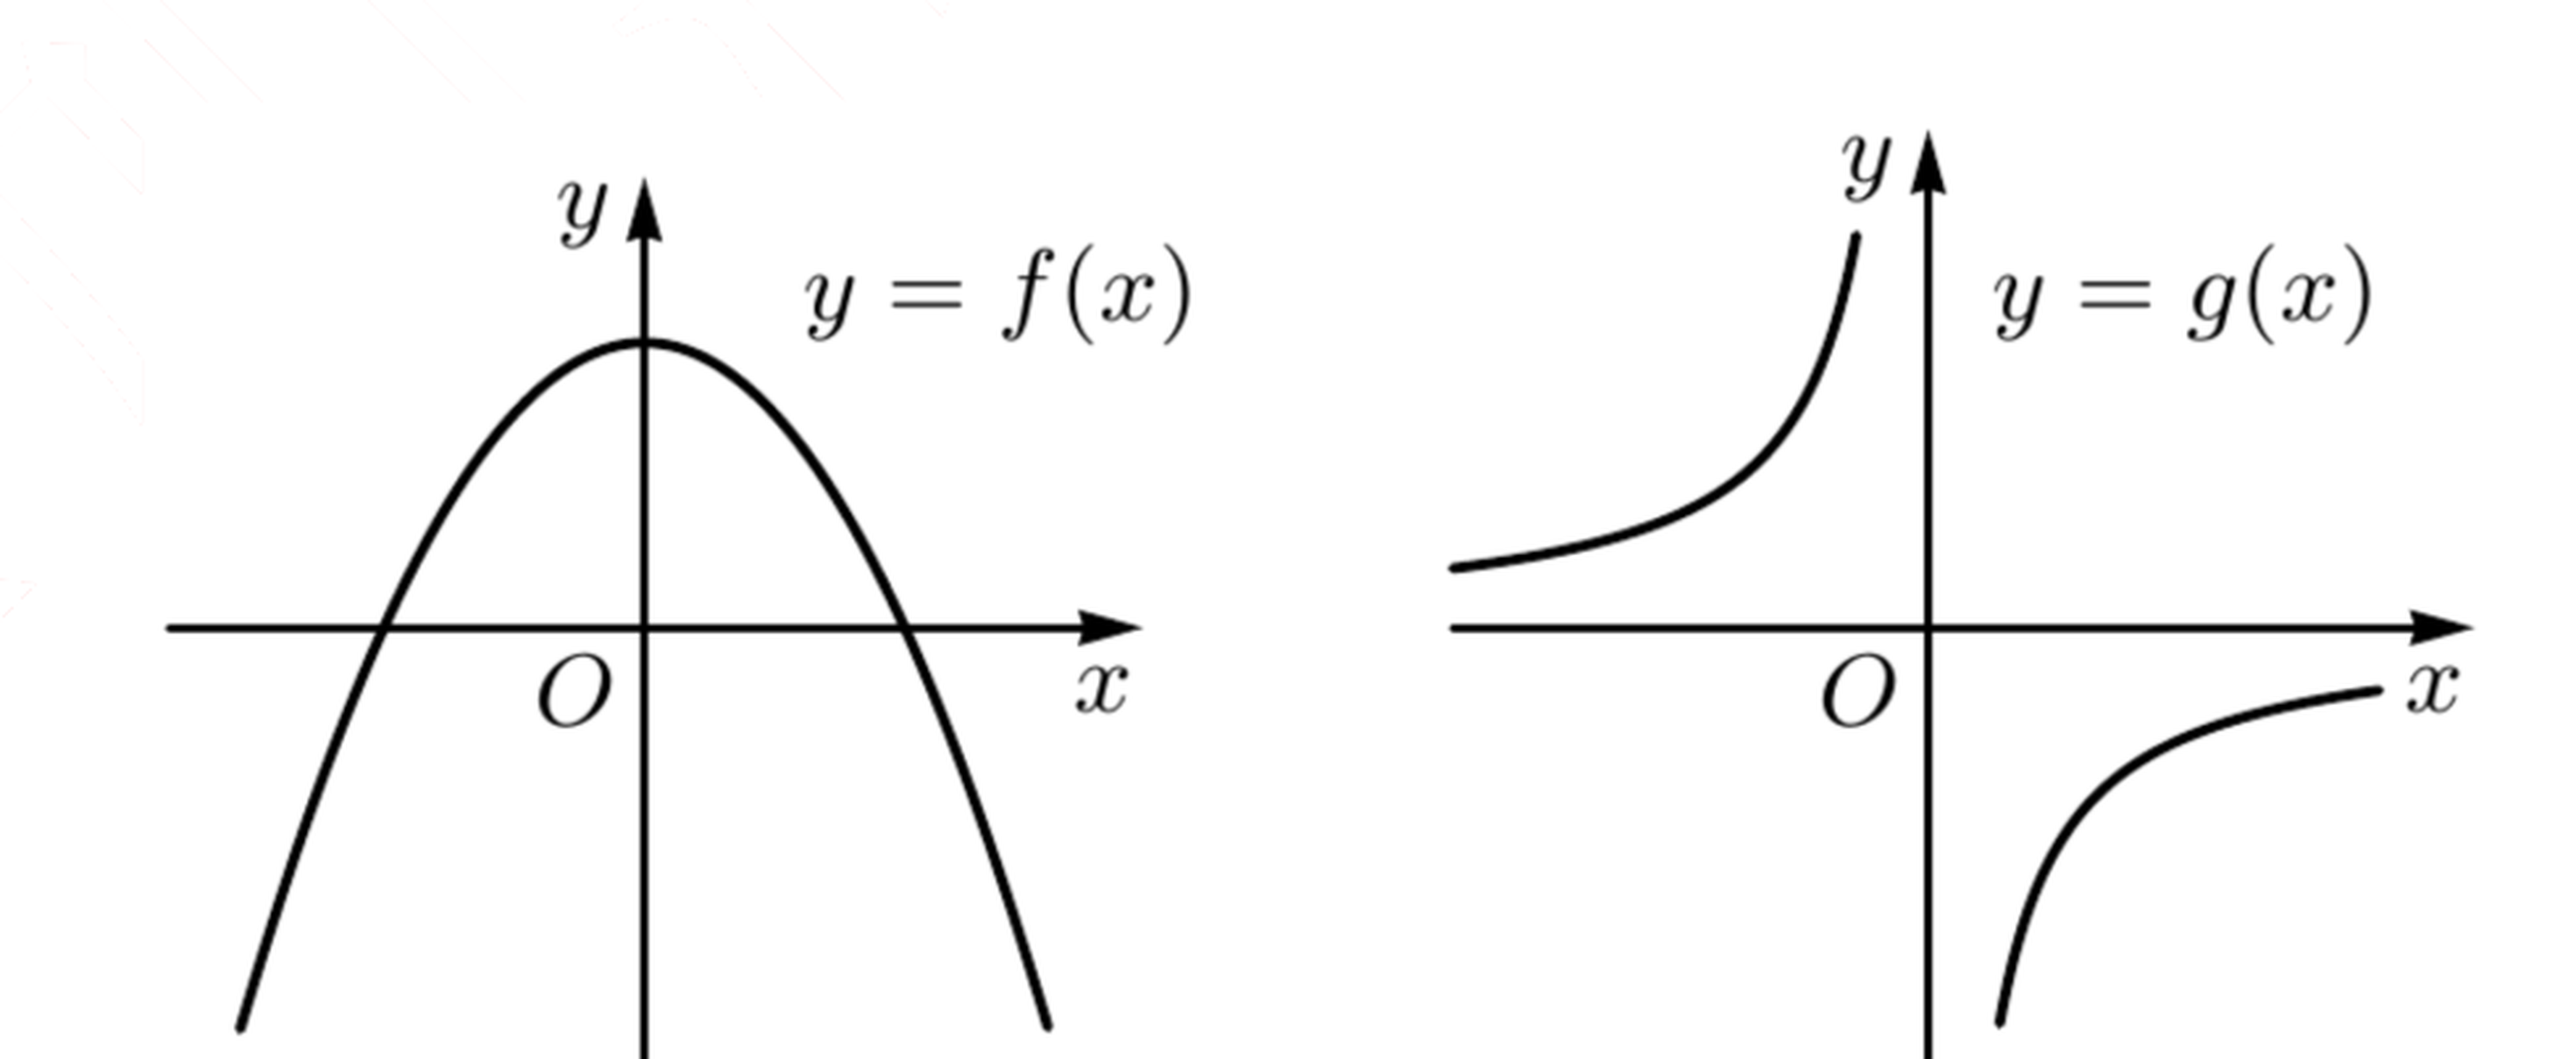
\includegraphics[width=0.72\textwidth]{figures/gao134_q13_graphs.png}\\[0.6em]
% A/B/C/D 四幅函数图象选项取原卷 04 页截图去粉色水印，按原卷一行四幅排布合并为一张
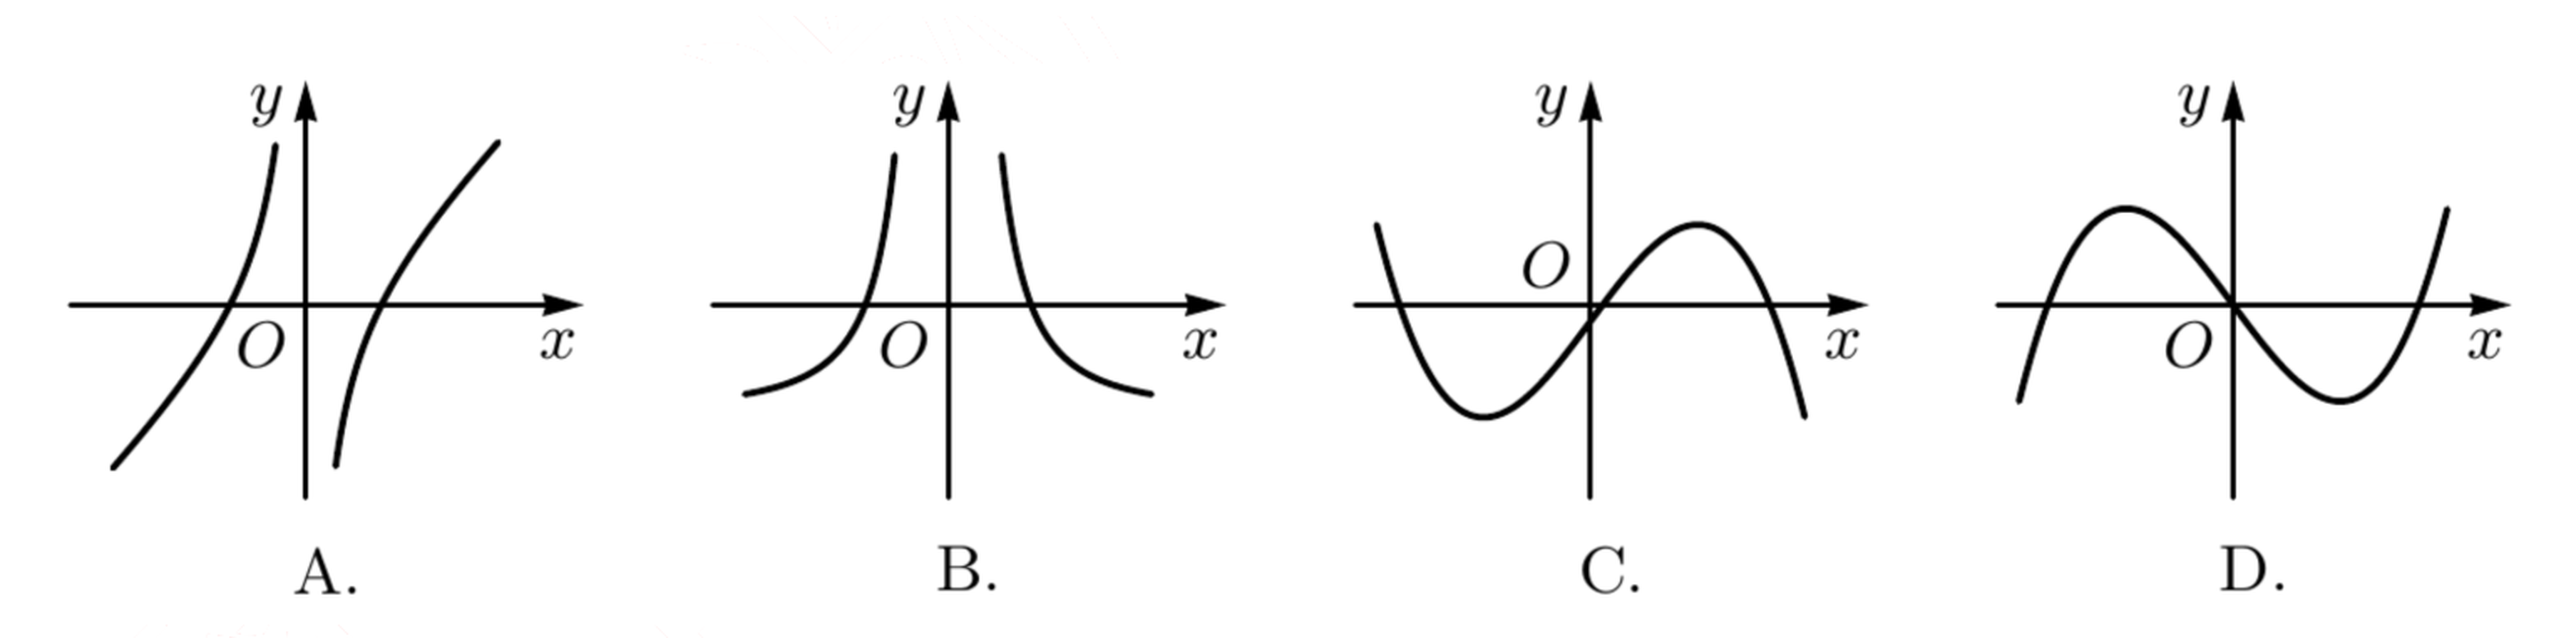
\includegraphics[width=0.90\textwidth]{figures/gao134_q13_options.png}
\end{center}

\ifanswer
\solbegin
\step{$f(x)$ 为偶函数，$g(x)$ 为奇函数，因此 $f(x)g(x)$ 为奇函数，排除 B.}
\step{又 $x=0$ 不在乘积函数的定义域内，其图象在 $y$ 轴上没有点，排除 C、D，}
\step{故选 $A$.}
\solend
\fi

\item 设全集为自然数集 $\N$，$E=\{x\mid x=2n,n\in\N\}$，$F=\{x\mid x=4n,n\in\N\}$，那么集合 $\N$ 可以表示成\mbox{（\quad）}

\keepwithprev
A. $E\cap F$\qquad\qquad B. $\overline{E}\cup F$\qquad\qquad C. $\overline{F}\cup E$\qquad\qquad D. $\overline{E}\cap\overline{F}$

\ifanswer
\solbegin
\step{$F\subseteq E$，所以 $\overline{F}\cup E=\N$，故选 $C$.}
\solend
\fi

\item 已知函数 $y=f(x)$，其中 $f(x)=x^2+bx$，则“$b<0$”是“$f(f(x))$ 的最小值与 $f(x)$ 的最小值相等”的\mbox{（\quad）}

\keepwithprev
A. 充分非必要条件\qquad\qquad B. 必要非充分条件

C. 充分必要条件\qquad\qquad D. 既非充分又非必要条件

\ifanswer
\solbegin
\step{$f(x)=\left(x+\dfrac b2\right)^2-\dfrac{b^2}4$，最小值为 $-\dfrac{b^2}4$，值域为 $\left[-\dfrac{b^2}4,+\infty\right)$.}
\step{当 $b<0$ 时，$-\dfrac b2>0\geqslant-\dfrac{b^2}4$，存在 $x$ 使 $f(x)=-\dfrac b2$，}
\step{从而 $f(f(x))$ 的最小值也为 $-\dfrac{b^2}4$，充分性成立.}
\step{当 $b=0$ 时，$f(x)=x^2$，$f(f(x))=x^4$，两者最小值均为 $0$，必要性不成立.}
\step{故选 $A$.}
\solend
\fi

\item 已知 $a,b,c\in\R$，若存在常数 $M>0$，使得 $a^2+b^2+c^2<M$，则称 $(a,b,c)$ 是有界数组. 对以下两个命题：

①若 $\lvert a^2+b+c\rvert+\lvert a^2+b-c\rvert\leqslant1$，则 $(a,b,c)$ 是有界数组；

②若 $\lvert a^2+b+c\rvert+\lvert a+b^2-c\rvert\leqslant1$，则 $(a,b,c)$ 是有界数组.% ②第二项为 \lvert a+b^2-c\rvert，与①刻意不同，照录

下列判断正确的是\mbox{（\quad）}

\keepwithprev
A. ①和②均为真命题\qquad\qquad B. ①和②均为假命题

C. ①为真命题，②为假命题\qquad D. ①为假命题，②为真命题

\ifanswer
\solbegin
\step{①取 $a=t,b=-t^2,c=0$，条件左端为 $0$，而 $a^2+b^2+c^2=t^2+t^4$ 可任意大，}
\step{故①为假命题.}
\step{②由条件，$a^2+a+b^2+b\leqslant\lvert a^2+b+c\rvert+\lvert a+b^2-c\rvert\leqslant1$.}
\step{由 $(a+1)^2+(b+1)^2\geqslant0$，得 $a^2+b^2\leqslant2(a^2+a+b^2+b)+2\leqslant4$.}
\step{又 $\lvert c\rvert\leqslant\lvert a^2+b+c\rvert+a^2+\lvert b\rvert\leqslant1+4+2=7$，故 $a^2+b^2+c^2\leqslant53<54$，}
\step{可取 $M=54$，故②为真命题.}
\step{故选 $D$.}
\solend
\fi

\end{enumerate}

\bigsec{三、解答题}

\begin{enumerate}
\setcounter{enumi}{16}

\item 已知不等式 $x^2-ax-b<0$ 的解集为 $A$，不等式 $\dfrac{3-2x}{x-1}<0$ 的解集为 $B$.

(1) 若 $a=5$，$b=-6$，求 $A\cap\overline{B}$；

(2) 若 $b=2a^2$，且 $A\cup B=B$，求实数 $a$ 的取值范围.

\ifanswer
\solbegin
\step{(1) 不等式 $\dfrac{3-2x}{x-1}<0$ 等价于 $x<1$ 或 $x>\dfrac32$，}
\step{所以 $B=(-\infty,1)\cup\left(\dfrac32,+\infty\right)$，$\overline{B}=\left[1,\dfrac32\right]$，}
\step{由 $x^2-5x+6=(x-2)(x-3)<0$，得 $A=(2,3)$，因此 $A\cap\overline{B}=\varnothing$.}
\step{(2) $A\cup B=B\Leftrightarrow A\subseteq B$，且 $x^2-ax-2a^2=(x-2a)(x+a)$，}
\step{当 $a=0$ 时，$A=\varnothing$，满足条件.}
\step{当 $a>0$ 时，$A=(-a,2a)$，$-a<0<1$，$A\subseteq B\Leftrightarrow2a\leqslant1$，得 $0<a\leqslant\dfrac12$.}
\step{当 $a<0$ 时，$A=(2a,-a)$，$2a<0<1$，$A\subseteq B\Leftrightarrow-a\leqslant1$，}
\step{得 $-1\leqslant a<0$.}
\step{因此 $a$ 的取值范围为 $\left[-1,\dfrac12\right]$.}
\solend
\fi

\item 为了在夏季降温和冬季供暖时减少能源损耗，房屋的屋顶和外墙需要建造隔热层. 某幢建筑物要建造可使用 $30$ 年的隔热层，每厘米厚的隔热层建造成本为 $9$ 万元. 该建筑物每年的能源消耗费用 $C$（万元）与隔热层厚度 $x$（cm）满足如下关系式：$C=\dfrac{k}{3x+5}$（$0\leqslant x\leqslant10$）. 若不建隔热层，每年能源消耗费用为 $8$ 万元. 设 $y$（万元）为隔热层建造费用与 $30$ 年的能源消耗费用之和.

(1) 求 $k$ 的值及 $y$ 的表达式；

(2) 隔热层修建多厚时，总费用 $y$ 最小？并求最小值.

\ifanswer
\solbegin
\step{(1) 不建隔热层时 $x=0$，$C=8$，所以 $\dfrac k5=8$，得 $k=40$.}
\step{隔热层建造费用为 $9x$ 万元，$30$ 年的能源消耗费用为 $30\times\dfrac{40}{3x+5}$ 万元.}
\step{因此 $y=9x+\dfrac{1200}{3x+5}$，$0\leqslant x\leqslant10$.}
\step{(2) 令 $t=3x+5$，则 $5\leqslant t\leqslant35$，且 $y=3t+\dfrac{1200}{t}-15$，}
\step{因为 $t>0$，由基本不等式得 $y\geqslant2\sqrt{3t\cdot\dfrac{1200}{t}}-15=105$，}
\step{当且仅当 $3t=\dfrac{1200}{t}$，即 $t=20$时取等号，此时 $x=5\in[0,10]$，}% 原卷"20"与"时"之间未留空，照录
\step{所以隔热层厚度为 $5$ cm 时，总费用最小，最小值为 $105$ 万元.}
\solend
\fi

\item 已知 $f(x)=ax^2+\dfrac1x$，其中 $a$ 为常数.

(1) 若 $a\in(1,3)$，判断函数 $y=f(x)$ 在 $[1,2]$ 上的单调性，并用定义证明；

(2) 求函数 $y=f(x)-x-\dfrac1x$ 在 $[1,2]$ 上的最大值 $g(a)$.

\ifanswer
\solbegin
\step{(1) 任取 $x_1,x_2\in[1,2]$，且 $x_1<x_2$，}
\step{则 $f(x_2)-f(x_1)=(x_2-x_1)\left[a(x_1+x_2)-\dfrac1{x_1x_2}\right]$，}
\step{由 $a>1$，$x_1+x_2\geqslant2$，$x_1x_2\geqslant1$，得 $a(x_1+x_2)-\dfrac1{x_1x_2}>2-1>0$，}
\step{因此 $f(x_2)>f(x_1)$，$f(x)$ 在 $[1,2]$ 上为严格增函数.}
\step{(2) 令 $h(x)=f(x)-x-\dfrac1x=ax^2-x$，其中 $x\in[1,2]$.}
\step{若 $a=0$，则 $h(x)=-x$，所以 $h(x)_{max}=h(1)=-1$；}
\step{若 $a<0$，二次函数的图象的对称轴为 $x=\dfrac1{2a}<0$，}
\step{所以 $y=h(x)$ 在 $[1,2]$ 上是严格减函数，所以 $h(x)_{max}=h(1)=a-1$；}
\step{若 $a>0$ 且 $\dfrac1{2a}>\dfrac32$，即 $0<a<\dfrac13$ 时，$h(x)_{max}=h(1)=a-1$.}
\step{若 $a>0$ 且 $\dfrac1{2a}\leqslant\dfrac32$，即 $a\geqslant\dfrac13$ 时，$h(x)_{max}=h(2)=4a-2$.}
\step{综上所述，$g(a)=\begin{cases}a-1,a<\dfrac13\\4a-2,a\geqslant\dfrac13\end{cases}$.}
\solend
\fi

\item 已知 $f(x)=\dfrac{ax^2+1}{bx+c}$（$a,b,c\in\Z$）.

(1) 若函数 $y=f(x)$ 是奇函数，且 $f(1)=2$，$f(2)<3$，求 $a,b,c$ 的值；

(2) 若函数 $y=f(x)$ 是偶函数，且 $ac<0$，$f(2a^2+a+1)<f(-3a^2+2a-1)$，求 $a$ 的值；

(3) 若 $b=a+c^2$，且满足不等式 $\lvert f(x)\rvert\geqslant1$ 的 $x$ 的最大值为 $0$，求 $c$ 的值.

\ifanswer
\solbegin
\step{(1) 由 $f(-x)=-f(x)$，交叉相乘得 $2c(ax^2+1)=0$ 恒成立，}
\step{因此 $c=0$，$b\neq0$.}
\step{由 $f(1)=2$，得 $a+1=2b$，}
\step{于是 $f(2)=\dfrac{4a+1}{2b}=4-\dfrac3{2b}<3\Leftrightarrow0<b<\dfrac32$，}
\step{因为 $b\in\Z$，所以 $b=1$，进而 $a=1$，$c=0$.}
\step{(2) 由 $f(-x)=f(x)$，交叉相乘得 $2bx(ax^2+1)=0$ 恒成立，因此 $b=0$.}
\step{此时 $f(x)=\dfrac ac x^2+\dfrac1c$，且 $\dfrac ac<0$.}
\step{设 $u=2a^2+a+1$，$v=-3a^2+2a-1$.}
\step{方程 $2a^2+a+1=0$ 与 $3a^2-2a+1=0$ 的判别式分别为 $-7$ 与 $-8$，}
\step{都小于 $0$，所以 $u>0$，$v<0$.}
\step{于是 $f(u)<f(v)\Leftrightarrow u^2>v^2\Leftrightarrow u>-v\Leftrightarrow-a^2+3a>0\Leftrightarrow0<a<3$，}
\step{因为 $a\in\Z$，所以 $a=1$ 或 $a=2$.}
\step{(3) 因为解集的最大值为 $0$，所以 $f(0)$ 有定义且 $\lvert f(0)\rvert\geqslant1$，}
\step{即 $c\neq0$，$\left\lvert\dfrac1c\right\rvert\geqslant1$，结合 $c\in\Z$，得 $c=\pm1$，从而 $b=a+1$.}
\step{当 $x=2$ 时，分母 $2a+2+c$ 为奇数，必不为 $0$；}
\step{又因为 $2>0$，必须有 $\lvert f(2)\rvert<1\Leftrightarrow\lvert4a+1\rvert<\lvert2a+2+c\rvert$，}
\step{若 $c=-1$，则 $(4a+1)^2<(2a+1)^2\Leftrightarrow4a(3a+1)<0\Leftrightarrow-\dfrac13<a<0$，}
\step{不存在满足条件的整数 $a$.}
\step{若 $c=1$，则 $(4a+1)^2<(2a+3)^2\Leftrightarrow4(3a+2)(a-1)<0\Leftrightarrow-\dfrac23<a<1$，}
\step{所以 $a=0$，$b=1$，此时 $f(x)=\dfrac1{x+1}$，}
\step{且 $\lvert f(x)\rvert\geqslant1\Leftrightarrow0<\lvert x+1\rvert\leqslant1\Leftrightarrow x\in[-2,-1)\cup(-1,0]$，}
\step{解集的最大值确为 $0$，因此 $c=1$.}
\solend
\fi

\item 已知函数 $y=f(x)$ 的定义域为 $\R$，且当 $x>0$ 时，$f(x)=\dfrac1{x+1}$. 对任意 $x_0\in\R$，定义集合 $D(x_0)=\{d\mid f(x_0+d)>f(x_0)\}$.

(1) 若当 $x\leqslant0$ 时，$f(x)=-2x+1$，求函数 $y=f(x)$ 的值域；

(2) 若 $y=f(x)$ 是偶函数，且 $f(0)=1$，求证：$D(-2)=\{-d\mid d\in D(2)\}$；

(3) 若 $y=f(x)$ 是奇函数，且 $x_1x_2\neq0$，求证：“$f(x_1)\leqslant f(x_2)$”的充要条件是\!\mbox{“$D(x_2)\subseteq D(x_1)$”}.

\ifanswer
\solbegin
\step{(1) 当 $x>0$ 时，$0<f(x)<1$；当 $x\leqslant0$ 时，$f(x)=-2x+1\geqslant1$.}
\step{函数的值域为 $(0,1)\cup[1,+\infty)=(0,+\infty)$.}
\step{(2) 由 $f(x)$ 是偶函数及 $f(0)=1$，得 $f(x)=\dfrac1{1+\lvert x\rvert}$，且 $f(2)=f(-2)=\dfrac13$.}
\stepm{法一：}{$D(2)=\left\{d\mid\dfrac1{1+\lvert2+d\rvert}>\dfrac13\right\}=\{d\mid\lvert2+d\rvert<2\}=(-4,0)$，}
\step{$D(-2)=\left\{d\mid\dfrac1{1+\lvert-2+d\rvert}>\dfrac13\right\}=\{d\mid\lvert-2+d\rvert<2\}=(0,4)$，}
\step{因此 $\{-d\mid d\in D(2)\}=(0,4)=D(-2)$.}
\stepm{法二：}{任取 $d\in D(-2)$，由定义得 $f(-2+d)>f(-2)$.}
\step{因为 $y=f(x)$ 是偶函数，所以对任意的实数 $x$，有 $f(-x)=f(x)$，}
\step{因此 $f(-2+d)=f(-(-2+d))=f(2-d)$，且 $f(-2)=f(2)$.}
\step{所以不等式 $f(-2+d)>f(-2)$ 等价于 $f(2-d)>f(2)$，}
\step{这恰好是 $-d\in D(2)$ 的定义，}
\step{所以 $d\in D(-2)\Leftrightarrow-d\in D(2)$，故 $D(-2)=\{-d\mid d\in D(2)\}$.}
\step{(3) 由 $f(x)$ 是奇函数，得 $f(0)=0$；}
\step{当 $x<0$ 时，$f(x)=-f(-x)=-\dfrac1{1-x}=\dfrac1{x-1}$；}
\step{所以 $f(x)=\begin{cases}\dfrac1{x-1},&x<0\\0,&x=0;\\\dfrac1{x+1},&x>0\end{cases}$}
% 2026-11-15 回原图订正：原卷 11 页此 cases 块末无句点，本稿初转顺手补了西文句点，今删去（Q19 08 页同类块末有句点，照录保留）。
\step{当 $x_0<0$ 时，$D(x_0)=\{d\mid f(x_0+d)>f(x_0)\}=(-\infty,0)\cup[-x_0,+\infty)$，}
\step{当 $x_0=0$ 时，$D(0)=\{d\mid f(0+d)>f(0)\}=(0,+\infty)$，}
\step{当 $x_0>0$ 时，$D(x_0)=\{d\mid f(x_0+d)>f(x_0)\}=(-x_0,0)$.}
\stepm{先证明必要性.}{若 $f(x_1)\leqslant f(x_2)$，仅需讨论三类情形：}
\step{若 $x_2\leqslant x_1<0$，}
\step{则 $D(x_1)=(-\infty,0)\cup[-x_1,+\infty),D(x_2)=(-\infty,0)\cup[-x_2,+\infty)$，}
\step{故 $D(x_2)\subseteq D(x_1)$；}
\step{若 $0<x_2\leqslant x_1$，则 $D(x_1)=(-x_1,0),D(x_2)=(-x_2,0)$，}
\step{故 $D(x_2)\subseteq D(x_1)$；}
\step{若 $x_1<0<x_2$，则 $D(x_1)=(-\infty,0)\cup[-x_1,+\infty),D(x_2)=(-x_2,0)$，}
\step{故 $D(x_2)\subseteq D(x_1)$.}
\stepm{再证明充分性.}{若 $D(x_2)\subseteq D(x_1)$，}
\step{若 $x_1<0,x_2<0$，}
\step{则 $D(x_1)=(-\infty,0)\cup[-x_1,+\infty),D(x_2)=(-\infty,0)\cup[-x_2,+\infty)$，}
\step{由 $D(x_2)\subseteq D(x_1)$ 得 $x_2\leqslant x_1$，}
\step{又 $y=f(x)$ 在 $(-\infty,0)$ 上是严格减函数，所以 $f(x_1)\leqslant f(x_2)$；}
\step{若 $x_1>0,x_2>0$，则 $D(x_1)=(-x_1,0),D(x_2)=(-x_2,0)$，}
\step{由 $D(x_2)\subseteq D(x_1)$ 得 $x_2\leqslant x_1$，}
\step{又 $y=f(x)$ 在 $(0,+\infty)$ 上是严格减函数，所以 $f(x_1)\leqslant f(x_2)$；}
\step{若 $x_1<0,x_2>0$，则 $f(x_1)<0<f(x_2)$，结论成立；}
\step{若 $x_1>0,x_2<0$，此时 $D(x_1)=(-x_1,0)$ 中只有负数，}
\step{而 $D(x_2)=(-\infty,0)\cup[-x_2,+\infty)$ 中有正数，$D(x_2)\subseteq D(x_1)$ 不成立.}
\step{综上，“$f(x_1)\leqslant f(x_2)$”的充要条件是“$D(x_2)\subseteq D(x_1)$”.}
\solend
\fi

\end{enumerate}

\end{document}
"
% 紧凑版：xelatex "\def\iscompact{1}% 高一134_华师大二附中_期中.tex
%   —— 高一上数学"2026-2027 年华师大二附中高一上期中"（试卷版/答案版）
% 试卷版：xelatex 高一134_华师大二附中_期中.tex
% 答案版：xelatex "\def\isanswer{1}\input{高一134_华师大二附中_期中.tex}"
% 紧凑版：xelatex "\def\iscompact{1}\input{高一134_华师大二附中_期中.tex}"
%
% ① 原始材料：微信公众号"魔都数学加油站"文章，作者破晓，2026-11-15 18:04 发布；
% 连载"27学年高一134"，原文标题"27学年高一134——2026-2027年上海市华师大二附中高一上期中"；
% 原文链接：https://mp.weixin.qq.com/s/bQlkmlGdCtAlytY331vf3g。
% 正文为 13 张 PNG 页（01、04、06、08、09、10、11、12、13 为 2560x3620；
% 02、03、05、07 为 4762x6735，同一篇各页分辨率不同，逐页按各自分辨率裁图核对），
% 题目下印有【解析】，为讲评版。题目、解析均据原图转录；卷面粉红色水印
% "魔都数学加油站"及公众号页脚未录入。
% 全卷 2 幅插图，均在第 04 页：第 13 题题干 y=f(x)、y=g(x) 两幅函数图象合并裁为
% figures/gao134_q13_graphs.png，第 13 题 A/B/C/D 四幅函数图象选项合并裁为
% figures/gao134_q13_options.png；两图均取原卷 04 页截图 3× LANCZOS 放大、
% 白化粉色水印（只白化浅粉色 R>175 且 G>140 且 B>140 的像素，保留红色标签）。
% 注意：本卷 Q13 四幅选项在原卷排为"一行四幅"（1×4），并非 高一132 第 14 题
% 的 2×2 排布，本稿按原卷 1×4 合并裁为一张，不重排、不用 TikZ 重绘。
%
% 卷首标题：原卷印作"2026-2027 年华师大二附中高一上期中"（公众号标题中的"上海市"
% 卷面标题行没有，本稿照卷面），年份区间按全稿惯例排 en dash；原卷未印副标题，
% 本卷为期中卷、跨集合与常用逻辑用语／不等式／函数三章，按题目内容标为
% "集合与常用逻辑用语、不等式、函数"（与 125／126／128／129／131／132／133 同期中卷口径相同）：
% 集合与逻辑见 Q6、Q10、Q14、Q16、Q17、Q21，不等式见 Q3、Q7、Q9、Q11、Q15、Q18、Q19，
% 函数（函数性质、二分法、奇偶性、基本不等式应用）见 Q4、Q5、Q8、Q12、Q13、Q20。
%
% 题号体例：本卷共 19 题——一、填空题 3—12（10 题）、二、选择题 13—16（4 题）、
% 三、解答题 17—21（5 题）。三节分别 \setcounter{enumi}{2}／{12}／{16}。
% 第 13 页仅为 Q21 (3) 解析续尾，全卷无「四、附加题」。
%
% ② 与原卷的排版差异：
%   ① 原文从第 3 题起，本稿保留原题号（见上"题号体例"）；
%   ② 原卷每题下直接印【解析】，本稿按全稿惯例置于答案版；第 13—16 题答案均在
%      解析末句"故选 …"，题干括号内留空、不另提 \ans{}（四题均无独立答案段）；
%      全卷无只印括号内答案、无解析的选择题；
%   ③ 原卷未印副标题，本稿按"知识模块"口径补出；
%   ④ 原卷填空横线按全稿惯例排为 \blankline[4.4em]；选择题括号排 \mbox{（\quad）}、
%      每个选项段前按惯例加 \keepwithprev（Q13 四选项为图，守卫前行为 \begin{center}；
%      Q15、Q16 四选项分两行排，\keepwithprev 只加在 A. 行前）；解答题不留作答区、
%      不加 \anspace（原卷为讲评版，与 129／131／132／133 同）；
%   ⑤ 原卷数集印黑板粗体（Q7／Q11／Q12／Q16／Q21 的 R、Q14／Q20 的 N、Q20 的 Z），
%      按全稿惯例统一排 \R／\N／\Z；绝对值排 \lvert…\rvert，集合描述竖线排 \mid；不等号按全稿惯例排
%      \leqslant／\geqslant；补集照原卷上划线排 \overline{B}、\overline{E}、\overline{F}；
%   ⑥ 子题标号 (1)(2)(3) 与括注原卷均用半角括号，照录（与 131／132／133 同）；
%      圈数字 ①② 照录；原卷 Q21 (2) 解析"法一：""法二："与 Q21 (3) 解析
%      "先证明必要性.""再证明充分性."四处标签印红色加粗，按 高一53／108／133 成例排
%      \stepm{法一：}／\stepm{法二：}／\stepm{先证明必要性.}／\stepm{再证明充分性.}
%      （加粗着色、不引入红色，不动 common.sty）；Q8 解析"第 1 步：""第 2 步：""
%      "第 3 步："原卷印黑色常规宋体（非红非粗），照录为普通 \step 行内文字；
%   ⑦ 数学式内半角逗号照录（如 Q6 $A=\{0,1,2,3\}$、Q14 $x=2n,n\in\N$、
%      Q16 $a,b,c\in\R$ 与 $a=t,b=-t^2,c=0$、Q19 $x_1,x_2\in[1,2]$、
%      Q20 $a,b,c\in\Z$、Q21 $x_1<0,x_2<0$ 与 $D(x_1)=(-x_1,0),D(x_2)=(-x_2,0)$）；
%      原卷行末全角句点按全稿惯例从宽排西文句点；cases 块末的句点逐处照录：
%      Q19 解析（08 页）块末原卷有句点照录、Q21 (3) 解析（11 页）块末原卷无句点不补，
%      两处原卷自身不统一（2026-11-15 回原图核对，本稿初转曾顺手补句点，已删去）；
%   ⑧ 原卷 Q8 解析跨 01—02 页、Q10 解析跨 02—03 页、Q12 解析跨 03—04 页、
%      Q16 解析跨 05—06 页、Q17 解析跨 06—07 页、Q20 解析跨 08—10 页、
%      Q21 解析跨 10—13 页，本稿按题合并连续排版；末页第 13 页为
%      Q21 (3) 解析续尾与"综上"一句，按实际印刷行单列；
%   ⑨ 题干中的中文弯引号按原卷照录（Q10 研究问题、Q15 条件、Q21 (3) 充要条件），
%      注释内一律 ASCII 引号。
%
% 判别式字形：全卷仅 Q9 解析末行出现一处判别式记号
%   "两值均满足 $\Delta=p^2-4p=18\mp12\sqrt2>0$"，逐处放大核对，原卷印高三角
%   $\Delta$（等腰、高，实测高宽比约 1.14），照录 \Delta；卷内无扁三角 \triangle，
%   与 高一132 同题排 $\triangle$、高一133 部分判别式排 $\triangle$ 均不同。
%
% 子集符号：Q6 题干 $C\subseteq A$、$C\subseteq B$ 与解析 $C\subseteq A\cap B$、
%   Q14 解析 $F\subseteq E$、Q17 解析 $A\subseteq B$、Q21 题干与解析各处的
%   $D(x_2)\subseteq D(x_1)$，全部印带下划线的 $\subseteq$，逐处放大核对，
%   照录 \subseteq；全卷未出现单线 \subset。
%
% 原卷存疑照录（均照录未改，正文对应处另有 % 注）：
%   第 6 题题干集合 $A=\{0,1,2,3\}$ 三个逗号后不留空，紧邻的 $B=\{0,2,4,5\}$
%      三个逗号后却留空，同卷同一行两集合排字不一，照录其逗号均为半角；
%   第 16 题命题②作 $\lvert a^2+b+c\rvert+\lvert a+b^2-c\rvert\leqslant1$，
%      与命题①第二项 $\lvert a^2+b-c\rvert$ 不同（①无 $b$ 的平方、②有），
%      两命题刻意不同，照录；解析"②由条件，$a^2+a+b^2+b\leqslant\cdots$"
%      由两项相加直接得到，照录；
%   第 18 题 (2) 解析"即 $t=20$时取等号"中"20"与"时"之间原卷未留空，照录；
%   第 19 题解析 $h(x)_{max}$ 的"max"下标三处字形不一（斜体／正体混排），照录；
%   第 20 题 (1)(2) 解析"由 $f(-x)=-f(x)$，交叉相乘得……"与"由 $f(-x)=f(x)$，
%      交叉相乘得……"两处措辞照录；
%   第 21 题 (2) 原卷并存"法一"（集合计算）与"法二"（定义推证）两套证明，照录不删。
%
% 行数复核：逐题数 \step/\stepm 条数，合计 134 条（Q3：2；Q4：1；Q5：1；Q6：1；
% Q7：2；Q8：4；Q9：3；Q10：4；Q11：5；Q12：8；Q13：3；Q14：1；Q15：5；
% Q16：7；Q17：9；Q18：7；Q19：11；Q20：22；Q21：38），与原卷印刷行逐题相等
% （cases 块作一个印刷行计）。第 13—16 题答案在解析末句，括号内留空、不另提 \ans{}；
% 第 21 题四条 \stepm 计入 38 条内。
%
\documentclass[a4paper,11pt]{article}
\usepackage{common}

\begin{document}

\examtitlest[3]{2026--2027 年华师大二附中高一上期中}{集合与常用逻辑用语、不等式、函数}

\bigsec{一、填空题}

\begin{enumerate}
\setcounter{enumi}{2}

\item 不等式 $\lvert 2x+1\rvert\geqslant3$ 的解集为\blankline[4.4em].

\ifanswer
\solbegin
\step{$\lvert 2x+1\rvert\geqslant3\Leftrightarrow 2x+1\leqslant-3$ 或 $2x+1\geqslant3\Leftrightarrow x\leqslant-2$ 或 $x\geqslant1$，}
\step{故解集为 $(-\infty,-2]\cup[1,+\infty)$.}
\solend
\fi

\item 函数 $y=\sqrt{x+1}+\dfrac1x$ 的定义域为\blankline[4.4em].

\ifanswer
\solbegin
\step{$x+1\geqslant0$ 且 $x\neq0$，得定义域为 $[-1,0)\cup(0,+\infty)$.}
\solend
\fi

\item 已知等式 $3x^2-4x-2=a(x-1)^2+b(x-1)+c$ 恒成立，其中 $a$、$b$、$c$ 为常数，则 $a-b+c=$\blankline[4.4em].

\ifanswer
\solbegin
\step{令 $x=0$，得 $a-b+c=-2$.}
\solend
\fi

\item 已知集合 $A=\{0,1,2,3\}$，$B=\{0,2,4,5\}$，$C\subseteq A$，$C\subseteq B$，符合条件的集合 $C$ 有\blankline[4.4em]个.% 原卷 A 的逗号后不留空、B 的逗号后留空，排字不一，照录

\ifanswer
\solbegin
\step{$C\subseteq A\cap B=\{0,2\}$，所以符合条件的集合 $C$ 有 $2^2=4$ 个.}
\solend
\fi

\item 设 $a$、$b\in\R$，且 $a^2+4b^2=2$，则 $ab$ 的最大值为\blankline[4.4em].

\ifanswer
\solbegin
\step{$(a-2b)^2=a^2+4b^2-4ab=2-4ab\geqslant0$，得 $ab\leqslant\dfrac12$，}
\step{当且仅当 $a=2b=\pm1$ 时取等号，故 $ab$ 的最大值为 $\dfrac12$.}
\solend
\fi

\item 已知函数 $y=x(13-2x)^2-140$，用二分法求函数在区间 $(3,4)$ 上的零点时，第 3 步应计算 $x=$\blankline[4.4em]的函数值.

\ifanswer
\solbegin
\step{记 $f(x)=x(13-2x)^2-140$，则 $f(3)=7>0$，$f(4)=-40<0$.}
\step{第 1 步：$f\left(\dfrac72\right)=-14<0$，区间缩小为 $\left(3,\dfrac72\right)$.}
\step{第 2 步：$f\left(\dfrac{13}4\right)=-\dfrac{43}{16}<0$，区间缩小为 $\left(3,\dfrac{13}4\right)$.}
\step{第 3 步：应计算 $x=\dfrac{3+\frac{13}4}2=\dfrac{25}8$ 的函数值.}
\solend
\fi

\item 已知一元二次方程 $x^2+px+p=0$ 的两个实根分别为 $x_1$、$x_2$，且 $x_1^2x_2+x_2^2x_1=-18$，则 $p=$\blankline[4.4em].% 判别式 \Delta 高三角，逐处放大核对

\ifanswer
\solbegin
\step{由韦达定理，$x_1+x_2=-p$，$x_1x_2=p$，}
\step{则 $x_1^2x_2+x_2^2x_1=x_1x_2(x_1+x_2)=-p^2=-18\Rightarrow p=\pm3\sqrt2$，}
\step{两值均满足 $\Delta=p^2-4p=18\mp12\sqrt2>0$，故 $p=\pm3\sqrt2$.}
\solend
\fi

\item 研究问题：“已知关于 $x$ 的不等式 $ax^2-bx+c>0$ 的解集为 $(1,2)$，解关于 $x$ 的不等式 $cx^2-bx+a>0$”，有如下解法：

解：由 $ax^2-bx+c>0\Rightarrow a-b\left(\dfrac1x\right)+c\left(\dfrac1x\right)^2>0$，令 $y=\dfrac1x$，则 $y\in\left(\dfrac12,1\right)$，

所以不等式 $cx^2-bx+a>0$ 的解集为 $\left(\dfrac12,1\right)$.

参考上述解法，已知关于 $x$ 的不等式 $\dfrac{k}{x+a}+\dfrac{x+b}{x+c}<0$ 的解集为 $(-3,-1)\cup(2,4)$，则关于 $x$ 的不等式 $\dfrac{kx}{ax-1}+\dfrac{bx-1}{cx-1}<0$ 的解集为\blankline[4.4em].

\ifanswer
\solbegin
\step{当 $x=0$ 时，所求不等式左端为 $1$，不满足不等式.}
\step{当 $x\neq0$ 时，两个分式的分子、分母同除以 $x$，得 $\dfrac{k}{a-\frac1x}+\dfrac{b-\frac1x}{c-\frac1x}<0$.}
\step{令 $t=-\dfrac1x$，则所求不等式化为 $\dfrac{k}{t+a}+\dfrac{t+b}{t+c}<0$，即 $-\dfrac1x\in(-3,-1)\cup(2,4)$，}
\step{解得 $x\in\left(-\dfrac12,-\dfrac14\right)\cup\left(\dfrac13,1\right)$.}
\solend
\fi

\item 已知 $a\in(0,+\infty)$，若对任意的 $x\in(0,+\infty)$，均有 $\lvert x^2-a\rvert+\lvert x+b\rvert=\lvert x^2+x-a+b\rvert$，则 $a^2-b^2$ 的最小值为\blankline[4.4em].

\ifanswer
\solbegin
\step{原等式成立的充要条件是 $(x^2-a)(x+b)\geqslant0$.}
\step{当 $0<x<\sqrt a$ 时须有 $x+b\leqslant0$；当 $x>\sqrt a$ 时须有 $x+b\geqslant0$，因此 $b=-\sqrt a$.}
\step{此时 $(x^2-a)(x+b)=(x+\sqrt a)(x-\sqrt a)^2\geqslant0$，满足题意.}
\step{$a^2-b^2=a^2-a=\left(a-\dfrac12\right)^2-\dfrac14\geqslant-\dfrac14$，}
\step{当 $a=\dfrac12$，$b=-\dfrac{\sqrt2}2$ 时取等号，最小值为 $-\dfrac14$.}
\solend
\fi

\item 已知函数 $y=f(x)$ 在 $\R$ 上是严格增函数，当 $x\neq0$ 且 $f(x)\neq0$ 时，满足 $f(x)\cdot f\left[\dfrac1{f(x)}+\dfrac1x\right]=1$，则 $f(1)=$\blankline[4.4em].

\ifanswer
\solbegin
\step{当 $xf(x)>0$ 时，记 $t=\dfrac1{f(x)}+\dfrac1x\neq0$，则 $f(t)=\dfrac1{f(x)}\neq0$.}
\step{将 $t$ 代入题设，得 $f\left(f(x)+\dfrac1t\right)=f(x)$，严格增性给出 $f(x)+\dfrac1t=x$，}
\step{化简得 $f(x)^2+xf(x)-x^2=0$，由 $\dfrac{f(x)}x>0$ 得 $f(x)=\dfrac{\sqrt5-1}2x$.}
\step{设 $a=f(0)$，若 $a>0$，则 $f(a)>f(0)=a>0$；}
\step{若 $a<0$，则 $f(a)<f(0)=a<0$.}
\step{两种情形都有 $af(a)>0$ 且 $\dfrac{f(a)}a>1$，与上式 $\dfrac{f(a)}a=\dfrac{\sqrt5-1}2<1$ 矛盾，}
\step{因此 $f(0)=0$.}
\step{于是 $f(1)>0$，代入上式得 $f(1)=\dfrac{\sqrt5-1}2$.}
\solend
\fi

\end{enumerate}

% 第 13 题是"节标题 + 题干 + 两幅图 + 四幅选项图"约 15cm 的整块，
% 守卫只放在 \bigsec 之前；若再在 \item 之前放第二枚，会在标题已印出后才触发换页，
% 把题目推走、留下孤立节标题（切页审计 B 类）。高度须覆盖整块。
\needvspace{16cm}
\bigsec{二、选择题}

\begin{enumerate}
\setcounter{enumi}{12}

\item 已知函数 $y=f(x)$ 与 $y=g(x)$ 的图象如图所示，则函数 $y=f(x)\cdot g(x)$ 的图象可能是\mbox{（\quad）}

\keepwithprev
\begin{center}
% 题干 y=f(x)、y=g(x) 两幅函数图象取原卷 04 页截图去粉色水印，按原卷左右排布合并为一张
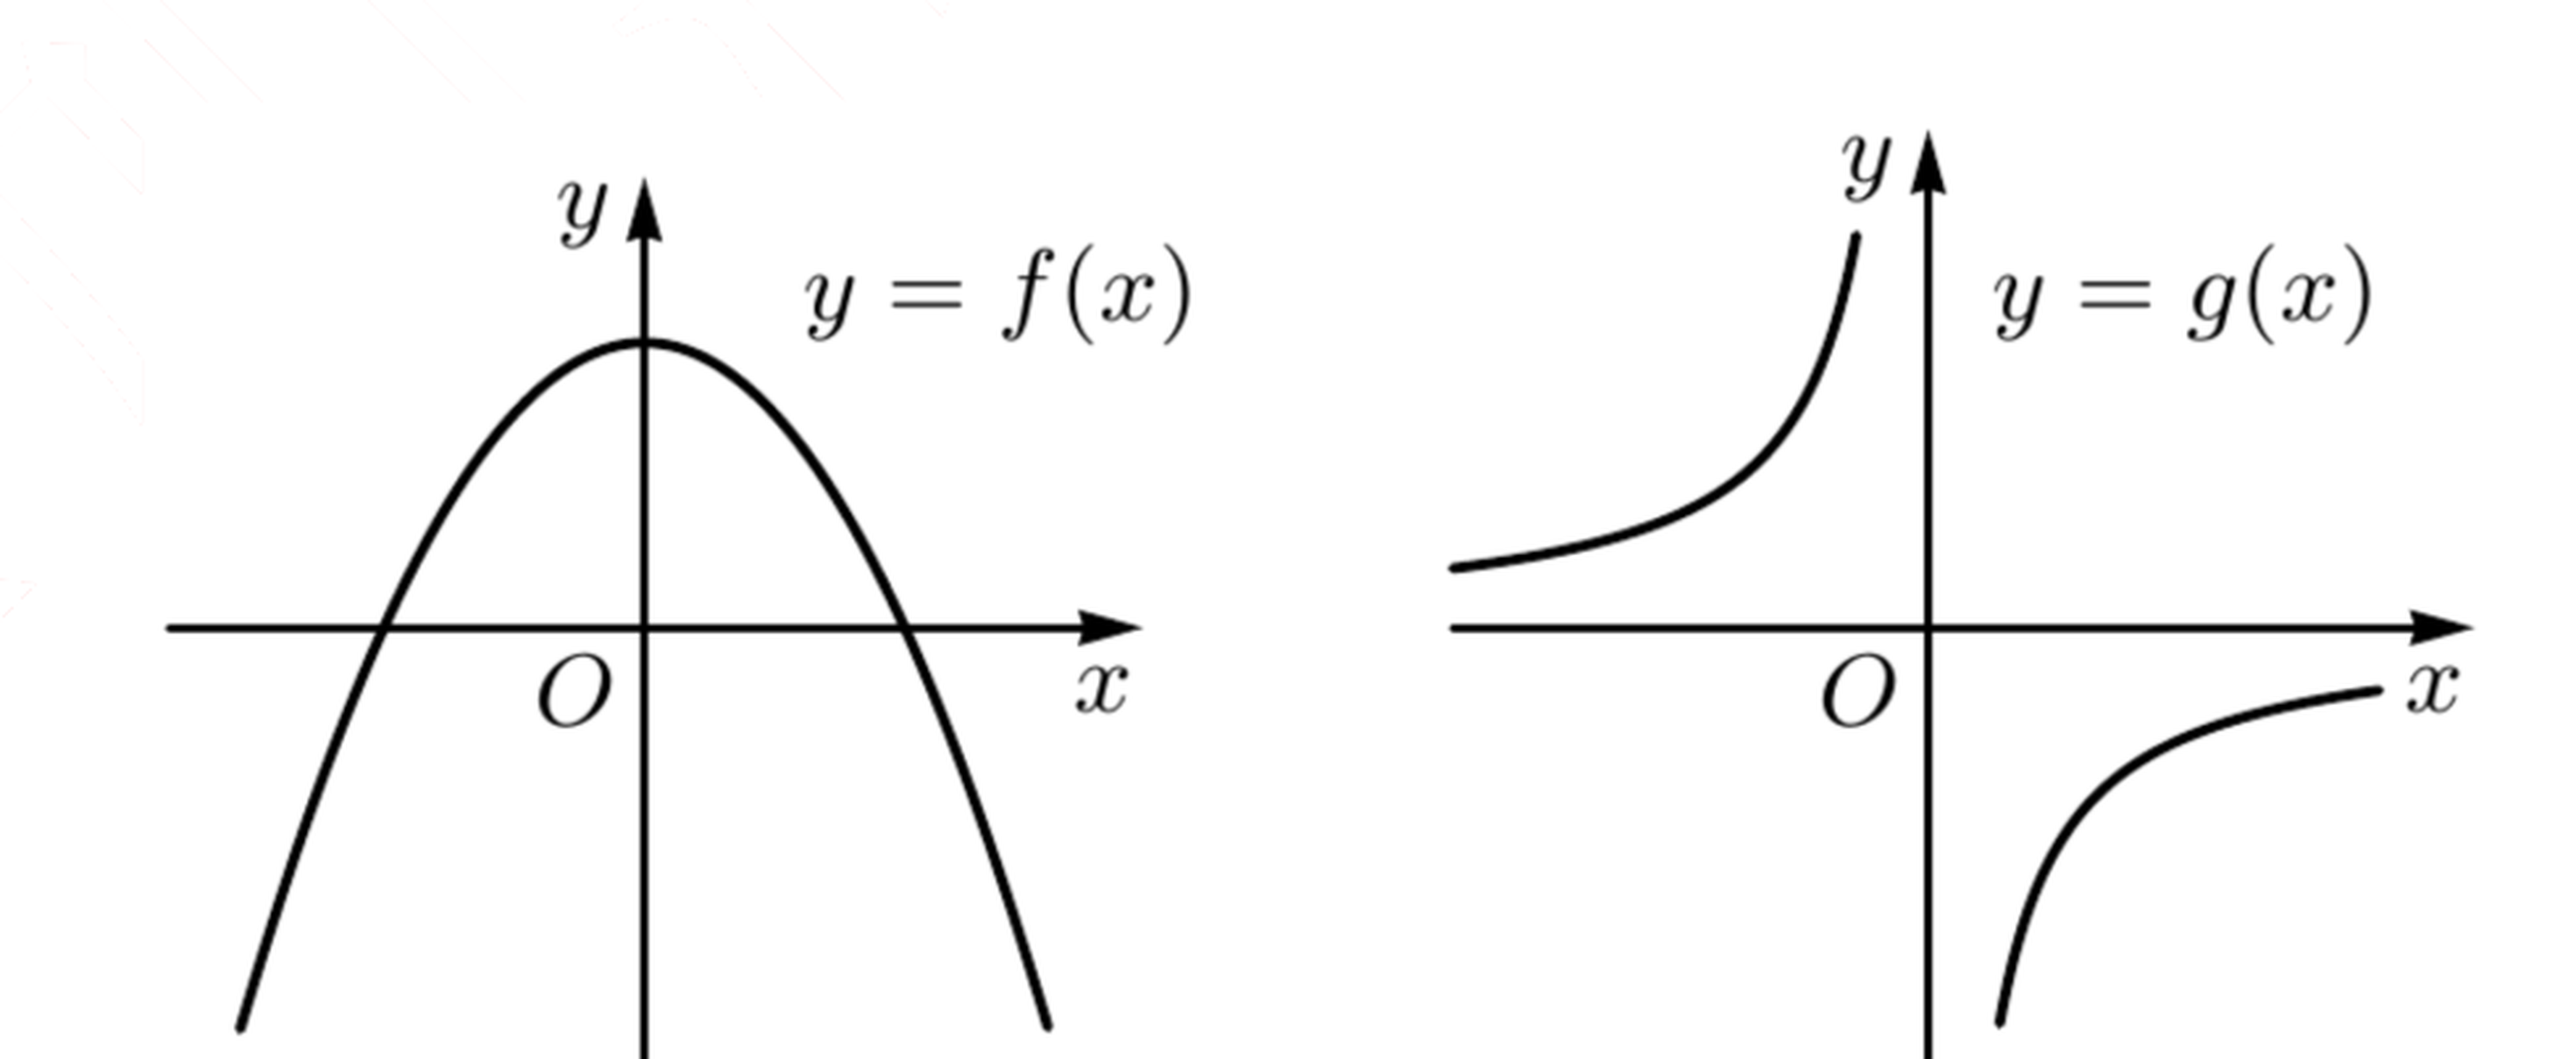
\includegraphics[width=0.72\textwidth]{figures/gao134_q13_graphs.png}\\[0.6em]
% A/B/C/D 四幅函数图象选项取原卷 04 页截图去粉色水印，按原卷一行四幅排布合并为一张
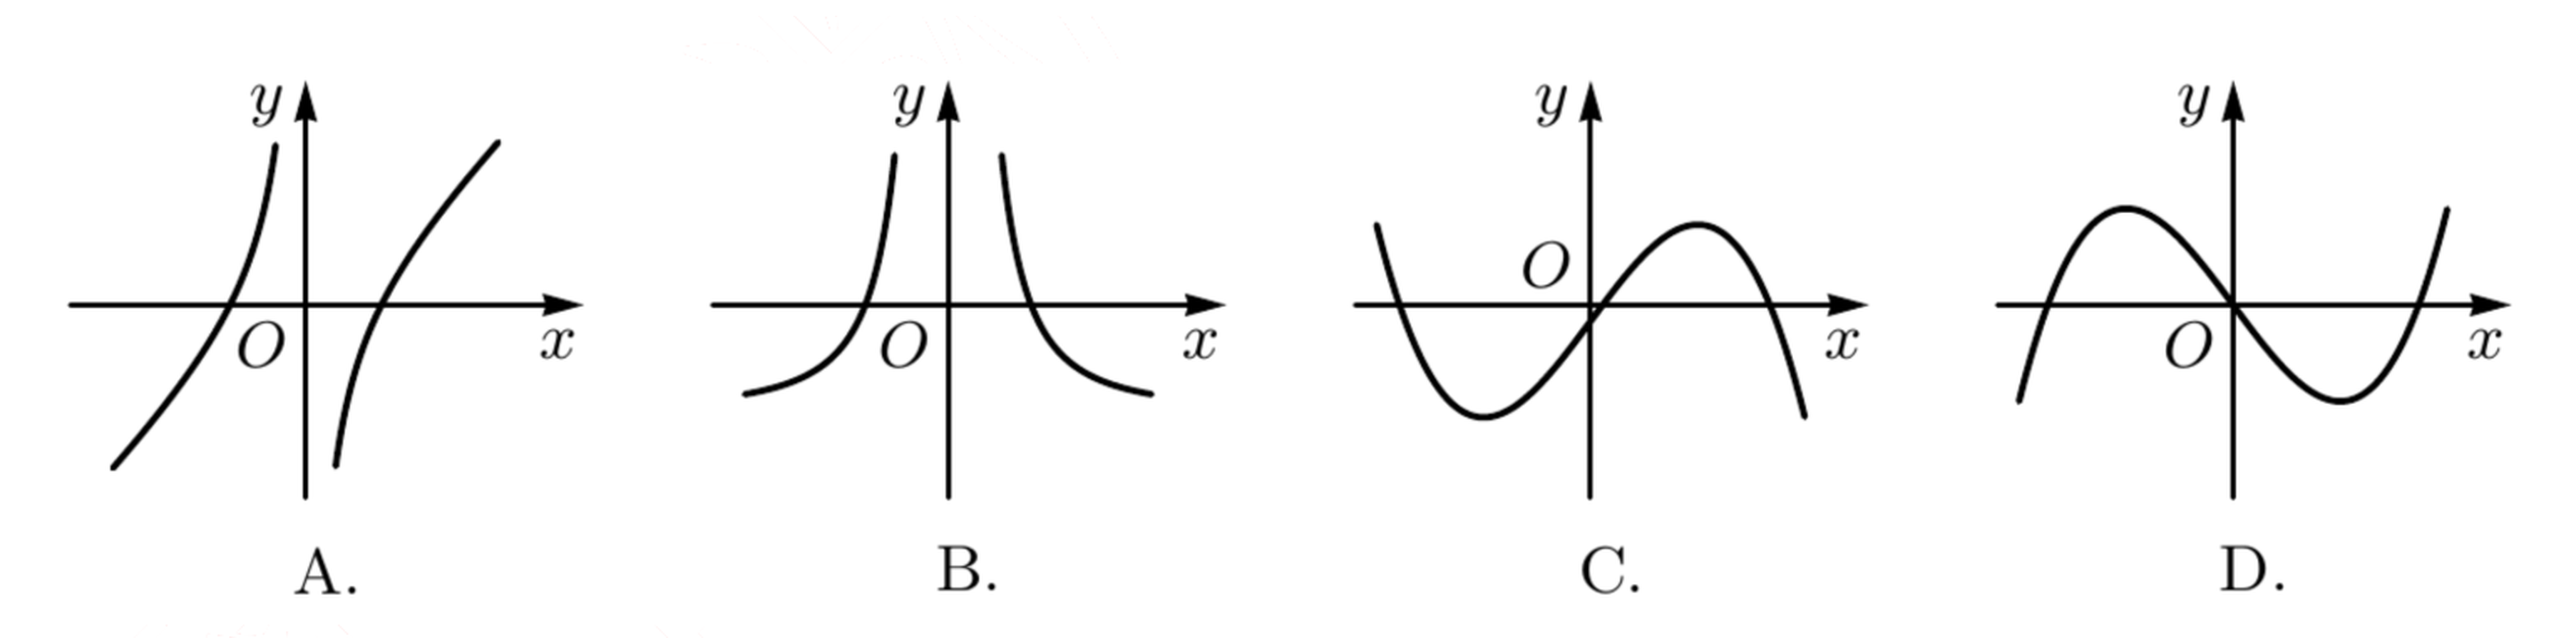
\includegraphics[width=0.90\textwidth]{figures/gao134_q13_options.png}
\end{center}

\ifanswer
\solbegin
\step{$f(x)$ 为偶函数，$g(x)$ 为奇函数，因此 $f(x)g(x)$ 为奇函数，排除 B.}
\step{又 $x=0$ 不在乘积函数的定义域内，其图象在 $y$ 轴上没有点，排除 C、D，}
\step{故选 $A$.}
\solend
\fi

\item 设全集为自然数集 $\N$，$E=\{x\mid x=2n,n\in\N\}$，$F=\{x\mid x=4n,n\in\N\}$，那么集合 $\N$ 可以表示成\mbox{（\quad）}

\keepwithprev
A. $E\cap F$\qquad\qquad B. $\overline{E}\cup F$\qquad\qquad C. $\overline{F}\cup E$\qquad\qquad D. $\overline{E}\cap\overline{F}$

\ifanswer
\solbegin
\step{$F\subseteq E$，所以 $\overline{F}\cup E=\N$，故选 $C$.}
\solend
\fi

\item 已知函数 $y=f(x)$，其中 $f(x)=x^2+bx$，则“$b<0$”是“$f(f(x))$ 的最小值与 $f(x)$ 的最小值相等”的\mbox{（\quad）}

\keepwithprev
A. 充分非必要条件\qquad\qquad B. 必要非充分条件

C. 充分必要条件\qquad\qquad D. 既非充分又非必要条件

\ifanswer
\solbegin
\step{$f(x)=\left(x+\dfrac b2\right)^2-\dfrac{b^2}4$，最小值为 $-\dfrac{b^2}4$，值域为 $\left[-\dfrac{b^2}4,+\infty\right)$.}
\step{当 $b<0$ 时，$-\dfrac b2>0\geqslant-\dfrac{b^2}4$，存在 $x$ 使 $f(x)=-\dfrac b2$，}
\step{从而 $f(f(x))$ 的最小值也为 $-\dfrac{b^2}4$，充分性成立.}
\step{当 $b=0$ 时，$f(x)=x^2$，$f(f(x))=x^4$，两者最小值均为 $0$，必要性不成立.}
\step{故选 $A$.}
\solend
\fi

\item 已知 $a,b,c\in\R$，若存在常数 $M>0$，使得 $a^2+b^2+c^2<M$，则称 $(a,b,c)$ 是有界数组. 对以下两个命题：

①若 $\lvert a^2+b+c\rvert+\lvert a^2+b-c\rvert\leqslant1$，则 $(a,b,c)$ 是有界数组；

②若 $\lvert a^2+b+c\rvert+\lvert a+b^2-c\rvert\leqslant1$，则 $(a,b,c)$ 是有界数组.% ②第二项为 \lvert a+b^2-c\rvert，与①刻意不同，照录

下列判断正确的是\mbox{（\quad）}

\keepwithprev
A. ①和②均为真命题\qquad\qquad B. ①和②均为假命题

C. ①为真命题，②为假命题\qquad D. ①为假命题，②为真命题

\ifanswer
\solbegin
\step{①取 $a=t,b=-t^2,c=0$，条件左端为 $0$，而 $a^2+b^2+c^2=t^2+t^4$ 可任意大，}
\step{故①为假命题.}
\step{②由条件，$a^2+a+b^2+b\leqslant\lvert a^2+b+c\rvert+\lvert a+b^2-c\rvert\leqslant1$.}
\step{由 $(a+1)^2+(b+1)^2\geqslant0$，得 $a^2+b^2\leqslant2(a^2+a+b^2+b)+2\leqslant4$.}
\step{又 $\lvert c\rvert\leqslant\lvert a^2+b+c\rvert+a^2+\lvert b\rvert\leqslant1+4+2=7$，故 $a^2+b^2+c^2\leqslant53<54$，}
\step{可取 $M=54$，故②为真命题.}
\step{故选 $D$.}
\solend
\fi

\end{enumerate}

\bigsec{三、解答题}

\begin{enumerate}
\setcounter{enumi}{16}

\item 已知不等式 $x^2-ax-b<0$ 的解集为 $A$，不等式 $\dfrac{3-2x}{x-1}<0$ 的解集为 $B$.

(1) 若 $a=5$，$b=-6$，求 $A\cap\overline{B}$；

(2) 若 $b=2a^2$，且 $A\cup B=B$，求实数 $a$ 的取值范围.

\ifanswer
\solbegin
\step{(1) 不等式 $\dfrac{3-2x}{x-1}<0$ 等价于 $x<1$ 或 $x>\dfrac32$，}
\step{所以 $B=(-\infty,1)\cup\left(\dfrac32,+\infty\right)$，$\overline{B}=\left[1,\dfrac32\right]$，}
\step{由 $x^2-5x+6=(x-2)(x-3)<0$，得 $A=(2,3)$，因此 $A\cap\overline{B}=\varnothing$.}
\step{(2) $A\cup B=B\Leftrightarrow A\subseteq B$，且 $x^2-ax-2a^2=(x-2a)(x+a)$，}
\step{当 $a=0$ 时，$A=\varnothing$，满足条件.}
\step{当 $a>0$ 时，$A=(-a,2a)$，$-a<0<1$，$A\subseteq B\Leftrightarrow2a\leqslant1$，得 $0<a\leqslant\dfrac12$.}
\step{当 $a<0$ 时，$A=(2a,-a)$，$2a<0<1$，$A\subseteq B\Leftrightarrow-a\leqslant1$，}
\step{得 $-1\leqslant a<0$.}
\step{因此 $a$ 的取值范围为 $\left[-1,\dfrac12\right]$.}
\solend
\fi

\item 为了在夏季降温和冬季供暖时减少能源损耗，房屋的屋顶和外墙需要建造隔热层. 某幢建筑物要建造可使用 $30$ 年的隔热层，每厘米厚的隔热层建造成本为 $9$ 万元. 该建筑物每年的能源消耗费用 $C$（万元）与隔热层厚度 $x$（cm）满足如下关系式：$C=\dfrac{k}{3x+5}$（$0\leqslant x\leqslant10$）. 若不建隔热层，每年能源消耗费用为 $8$ 万元. 设 $y$（万元）为隔热层建造费用与 $30$ 年的能源消耗费用之和.

(1) 求 $k$ 的值及 $y$ 的表达式；

(2) 隔热层修建多厚时，总费用 $y$ 最小？并求最小值.

\ifanswer
\solbegin
\step{(1) 不建隔热层时 $x=0$，$C=8$，所以 $\dfrac k5=8$，得 $k=40$.}
\step{隔热层建造费用为 $9x$ 万元，$30$ 年的能源消耗费用为 $30\times\dfrac{40}{3x+5}$ 万元.}
\step{因此 $y=9x+\dfrac{1200}{3x+5}$，$0\leqslant x\leqslant10$.}
\step{(2) 令 $t=3x+5$，则 $5\leqslant t\leqslant35$，且 $y=3t+\dfrac{1200}{t}-15$，}
\step{因为 $t>0$，由基本不等式得 $y\geqslant2\sqrt{3t\cdot\dfrac{1200}{t}}-15=105$，}
\step{当且仅当 $3t=\dfrac{1200}{t}$，即 $t=20$时取等号，此时 $x=5\in[0,10]$，}% 原卷"20"与"时"之间未留空，照录
\step{所以隔热层厚度为 $5$ cm 时，总费用最小，最小值为 $105$ 万元.}
\solend
\fi

\item 已知 $f(x)=ax^2+\dfrac1x$，其中 $a$ 为常数.

(1) 若 $a\in(1,3)$，判断函数 $y=f(x)$ 在 $[1,2]$ 上的单调性，并用定义证明；

(2) 求函数 $y=f(x)-x-\dfrac1x$ 在 $[1,2]$ 上的最大值 $g(a)$.

\ifanswer
\solbegin
\step{(1) 任取 $x_1,x_2\in[1,2]$，且 $x_1<x_2$，}
\step{则 $f(x_2)-f(x_1)=(x_2-x_1)\left[a(x_1+x_2)-\dfrac1{x_1x_2}\right]$，}
\step{由 $a>1$，$x_1+x_2\geqslant2$，$x_1x_2\geqslant1$，得 $a(x_1+x_2)-\dfrac1{x_1x_2}>2-1>0$，}
\step{因此 $f(x_2)>f(x_1)$，$f(x)$ 在 $[1,2]$ 上为严格增函数.}
\step{(2) 令 $h(x)=f(x)-x-\dfrac1x=ax^2-x$，其中 $x\in[1,2]$.}
\step{若 $a=0$，则 $h(x)=-x$，所以 $h(x)_{max}=h(1)=-1$；}
\step{若 $a<0$，二次函数的图象的对称轴为 $x=\dfrac1{2a}<0$，}
\step{所以 $y=h(x)$ 在 $[1,2]$ 上是严格减函数，所以 $h(x)_{max}=h(1)=a-1$；}
\step{若 $a>0$ 且 $\dfrac1{2a}>\dfrac32$，即 $0<a<\dfrac13$ 时，$h(x)_{max}=h(1)=a-1$.}
\step{若 $a>0$ 且 $\dfrac1{2a}\leqslant\dfrac32$，即 $a\geqslant\dfrac13$ 时，$h(x)_{max}=h(2)=4a-2$.}
\step{综上所述，$g(a)=\begin{cases}a-1,a<\dfrac13\\4a-2,a\geqslant\dfrac13\end{cases}$.}
\solend
\fi

\item 已知 $f(x)=\dfrac{ax^2+1}{bx+c}$（$a,b,c\in\Z$）.

(1) 若函数 $y=f(x)$ 是奇函数，且 $f(1)=2$，$f(2)<3$，求 $a,b,c$ 的值；

(2) 若函数 $y=f(x)$ 是偶函数，且 $ac<0$，$f(2a^2+a+1)<f(-3a^2+2a-1)$，求 $a$ 的值；

(3) 若 $b=a+c^2$，且满足不等式 $\lvert f(x)\rvert\geqslant1$ 的 $x$ 的最大值为 $0$，求 $c$ 的值.

\ifanswer
\solbegin
\step{(1) 由 $f(-x)=-f(x)$，交叉相乘得 $2c(ax^2+1)=0$ 恒成立，}
\step{因此 $c=0$，$b\neq0$.}
\step{由 $f(1)=2$，得 $a+1=2b$，}
\step{于是 $f(2)=\dfrac{4a+1}{2b}=4-\dfrac3{2b}<3\Leftrightarrow0<b<\dfrac32$，}
\step{因为 $b\in\Z$，所以 $b=1$，进而 $a=1$，$c=0$.}
\step{(2) 由 $f(-x)=f(x)$，交叉相乘得 $2bx(ax^2+1)=0$ 恒成立，因此 $b=0$.}
\step{此时 $f(x)=\dfrac ac x^2+\dfrac1c$，且 $\dfrac ac<0$.}
\step{设 $u=2a^2+a+1$，$v=-3a^2+2a-1$.}
\step{方程 $2a^2+a+1=0$ 与 $3a^2-2a+1=0$ 的判别式分别为 $-7$ 与 $-8$，}
\step{都小于 $0$，所以 $u>0$，$v<0$.}
\step{于是 $f(u)<f(v)\Leftrightarrow u^2>v^2\Leftrightarrow u>-v\Leftrightarrow-a^2+3a>0\Leftrightarrow0<a<3$，}
\step{因为 $a\in\Z$，所以 $a=1$ 或 $a=2$.}
\step{(3) 因为解集的最大值为 $0$，所以 $f(0)$ 有定义且 $\lvert f(0)\rvert\geqslant1$，}
\step{即 $c\neq0$，$\left\lvert\dfrac1c\right\rvert\geqslant1$，结合 $c\in\Z$，得 $c=\pm1$，从而 $b=a+1$.}
\step{当 $x=2$ 时，分母 $2a+2+c$ 为奇数，必不为 $0$；}
\step{又因为 $2>0$，必须有 $\lvert f(2)\rvert<1\Leftrightarrow\lvert4a+1\rvert<\lvert2a+2+c\rvert$，}
\step{若 $c=-1$，则 $(4a+1)^2<(2a+1)^2\Leftrightarrow4a(3a+1)<0\Leftrightarrow-\dfrac13<a<0$，}
\step{不存在满足条件的整数 $a$.}
\step{若 $c=1$，则 $(4a+1)^2<(2a+3)^2\Leftrightarrow4(3a+2)(a-1)<0\Leftrightarrow-\dfrac23<a<1$，}
\step{所以 $a=0$，$b=1$，此时 $f(x)=\dfrac1{x+1}$，}
\step{且 $\lvert f(x)\rvert\geqslant1\Leftrightarrow0<\lvert x+1\rvert\leqslant1\Leftrightarrow x\in[-2,-1)\cup(-1,0]$，}
\step{解集的最大值确为 $0$，因此 $c=1$.}
\solend
\fi

\item 已知函数 $y=f(x)$ 的定义域为 $\R$，且当 $x>0$ 时，$f(x)=\dfrac1{x+1}$. 对任意 $x_0\in\R$，定义集合 $D(x_0)=\{d\mid f(x_0+d)>f(x_0)\}$.

(1) 若当 $x\leqslant0$ 时，$f(x)=-2x+1$，求函数 $y=f(x)$ 的值域；

(2) 若 $y=f(x)$ 是偶函数，且 $f(0)=1$，求证：$D(-2)=\{-d\mid d\in D(2)\}$；

(3) 若 $y=f(x)$ 是奇函数，且 $x_1x_2\neq0$，求证：“$f(x_1)\leqslant f(x_2)$”的充要条件是\!\mbox{“$D(x_2)\subseteq D(x_1)$”}.

\ifanswer
\solbegin
\step{(1) 当 $x>0$ 时，$0<f(x)<1$；当 $x\leqslant0$ 时，$f(x)=-2x+1\geqslant1$.}
\step{函数的值域为 $(0,1)\cup[1,+\infty)=(0,+\infty)$.}
\step{(2) 由 $f(x)$ 是偶函数及 $f(0)=1$，得 $f(x)=\dfrac1{1+\lvert x\rvert}$，且 $f(2)=f(-2)=\dfrac13$.}
\stepm{法一：}{$D(2)=\left\{d\mid\dfrac1{1+\lvert2+d\rvert}>\dfrac13\right\}=\{d\mid\lvert2+d\rvert<2\}=(-4,0)$，}
\step{$D(-2)=\left\{d\mid\dfrac1{1+\lvert-2+d\rvert}>\dfrac13\right\}=\{d\mid\lvert-2+d\rvert<2\}=(0,4)$，}
\step{因此 $\{-d\mid d\in D(2)\}=(0,4)=D(-2)$.}
\stepm{法二：}{任取 $d\in D(-2)$，由定义得 $f(-2+d)>f(-2)$.}
\step{因为 $y=f(x)$ 是偶函数，所以对任意的实数 $x$，有 $f(-x)=f(x)$，}
\step{因此 $f(-2+d)=f(-(-2+d))=f(2-d)$，且 $f(-2)=f(2)$.}
\step{所以不等式 $f(-2+d)>f(-2)$ 等价于 $f(2-d)>f(2)$，}
\step{这恰好是 $-d\in D(2)$ 的定义，}
\step{所以 $d\in D(-2)\Leftrightarrow-d\in D(2)$，故 $D(-2)=\{-d\mid d\in D(2)\}$.}
\step{(3) 由 $f(x)$ 是奇函数，得 $f(0)=0$；}
\step{当 $x<0$ 时，$f(x)=-f(-x)=-\dfrac1{1-x}=\dfrac1{x-1}$；}
\step{所以 $f(x)=\begin{cases}\dfrac1{x-1},&x<0\\0,&x=0;\\\dfrac1{x+1},&x>0\end{cases}$}
% 2026-11-15 回原图订正：原卷 11 页此 cases 块末无句点，本稿初转顺手补了西文句点，今删去（Q19 08 页同类块末有句点，照录保留）。
\step{当 $x_0<0$ 时，$D(x_0)=\{d\mid f(x_0+d)>f(x_0)\}=(-\infty,0)\cup[-x_0,+\infty)$，}
\step{当 $x_0=0$ 时，$D(0)=\{d\mid f(0+d)>f(0)\}=(0,+\infty)$，}
\step{当 $x_0>0$ 时，$D(x_0)=\{d\mid f(x_0+d)>f(x_0)\}=(-x_0,0)$.}
\stepm{先证明必要性.}{若 $f(x_1)\leqslant f(x_2)$，仅需讨论三类情形：}
\step{若 $x_2\leqslant x_1<0$，}
\step{则 $D(x_1)=(-\infty,0)\cup[-x_1,+\infty),D(x_2)=(-\infty,0)\cup[-x_2,+\infty)$，}
\step{故 $D(x_2)\subseteq D(x_1)$；}
\step{若 $0<x_2\leqslant x_1$，则 $D(x_1)=(-x_1,0),D(x_2)=(-x_2,0)$，}
\step{故 $D(x_2)\subseteq D(x_1)$；}
\step{若 $x_1<0<x_2$，则 $D(x_1)=(-\infty,0)\cup[-x_1,+\infty),D(x_2)=(-x_2,0)$，}
\step{故 $D(x_2)\subseteq D(x_1)$.}
\stepm{再证明充分性.}{若 $D(x_2)\subseteq D(x_1)$，}
\step{若 $x_1<0,x_2<0$，}
\step{则 $D(x_1)=(-\infty,0)\cup[-x_1,+\infty),D(x_2)=(-\infty,0)\cup[-x_2,+\infty)$，}
\step{由 $D(x_2)\subseteq D(x_1)$ 得 $x_2\leqslant x_1$，}
\step{又 $y=f(x)$ 在 $(-\infty,0)$ 上是严格减函数，所以 $f(x_1)\leqslant f(x_2)$；}
\step{若 $x_1>0,x_2>0$，则 $D(x_1)=(-x_1,0),D(x_2)=(-x_2,0)$，}
\step{由 $D(x_2)\subseteq D(x_1)$ 得 $x_2\leqslant x_1$，}
\step{又 $y=f(x)$ 在 $(0,+\infty)$ 上是严格减函数，所以 $f(x_1)\leqslant f(x_2)$；}
\step{若 $x_1<0,x_2>0$，则 $f(x_1)<0<f(x_2)$，结论成立；}
\step{若 $x_1>0,x_2<0$，此时 $D(x_1)=(-x_1,0)$ 中只有负数，}
\step{而 $D(x_2)=(-\infty,0)\cup[-x_2,+\infty)$ 中有正数，$D(x_2)\subseteq D(x_1)$ 不成立.}
\step{综上，“$f(x_1)\leqslant f(x_2)$”的充要条件是“$D(x_2)\subseteq D(x_1)$”.}
\solend
\fi

\end{enumerate}

\end{document}
"
%
% ① 原始材料：微信公众号"魔都数学加油站"文章，作者破晓，2026-11-15 18:04 发布；
% 连载"27学年高一134"，原文标题"27学年高一134——2026-2027年上海市华师大二附中高一上期中"；
% 原文链接：https://mp.weixin.qq.com/s/bQlkmlGdCtAlytY331vf3g。
% 正文为 13 张 PNG 页（01、04、06、08、09、10、11、12、13 为 2560x3620；
% 02、03、05、07 为 4762x6735，同一篇各页分辨率不同，逐页按各自分辨率裁图核对），
% 题目下印有【解析】，为讲评版。题目、解析均据原图转录；卷面粉红色水印
% "魔都数学加油站"及公众号页脚未录入。
% 全卷 2 幅插图，均在第 04 页：第 13 题题干 y=f(x)、y=g(x) 两幅函数图象合并裁为
% figures/gao134_q13_graphs.png，第 13 题 A/B/C/D 四幅函数图象选项合并裁为
% figures/gao134_q13_options.png；两图均取原卷 04 页截图 3× LANCZOS 放大、
% 白化粉色水印（只白化浅粉色 R>175 且 G>140 且 B>140 的像素，保留红色标签）。
% 注意：本卷 Q13 四幅选项在原卷排为"一行四幅"（1×4），并非 高一132 第 14 题
% 的 2×2 排布，本稿按原卷 1×4 合并裁为一张，不重排、不用 TikZ 重绘。
%
% 卷首标题：原卷印作"2026-2027 年华师大二附中高一上期中"（公众号标题中的"上海市"
% 卷面标题行没有，本稿照卷面），年份区间按全稿惯例排 en dash；原卷未印副标题，
% 本卷为期中卷、跨集合与常用逻辑用语／不等式／函数三章，按题目内容标为
% "集合与常用逻辑用语、不等式、函数"（与 125／126／128／129／131／132／133 同期中卷口径相同）：
% 集合与逻辑见 Q6、Q10、Q14、Q16、Q17、Q21，不等式见 Q3、Q7、Q9、Q11、Q15、Q18、Q19，
% 函数（函数性质、二分法、奇偶性、基本不等式应用）见 Q4、Q5、Q8、Q12、Q13、Q20。
%
% 题号体例：本卷共 19 题——一、填空题 3—12（10 题）、二、选择题 13—16（4 题）、
% 三、解答题 17—21（5 题）。三节分别 \setcounter{enumi}{2}／{12}／{16}。
% 第 13 页仅为 Q21 (3) 解析续尾，全卷无「四、附加题」。
%
% ② 与原卷的排版差异：
%   ① 原文从第 3 题起，本稿保留原题号（见上"题号体例"）；
%   ② 原卷每题下直接印【解析】，本稿按全稿惯例置于答案版；第 13—16 题答案均在
%      解析末句"故选 …"，题干括号内留空、不另提 \ans{}（四题均无独立答案段）；
%      全卷无只印括号内答案、无解析的选择题；
%   ③ 原卷未印副标题，本稿按"知识模块"口径补出；
%   ④ 原卷填空横线按全稿惯例排为 \blankline[4.4em]；选择题括号排 \mbox{（\quad）}、
%      每个选项段前按惯例加 \keepwithprev（Q13 四选项为图，守卫前行为 \begin{center}；
%      Q15、Q16 四选项分两行排，\keepwithprev 只加在 A. 行前）；解答题不留作答区、
%      不加 \anspace（原卷为讲评版，与 129／131／132／133 同）；
%   ⑤ 原卷数集印黑板粗体（Q7／Q11／Q12／Q16／Q21 的 R、Q14／Q20 的 N、Q20 的 Z），
%      按全稿惯例统一排 \R／\N／\Z；绝对值排 \lvert…\rvert，集合描述竖线排 \mid；不等号按全稿惯例排
%      \leqslant／\geqslant；补集照原卷上划线排 \overline{B}、\overline{E}、\overline{F}；
%   ⑥ 子题标号 (1)(2)(3) 与括注原卷均用半角括号，照录（与 131／132／133 同）；
%      圈数字 ①② 照录；原卷 Q21 (2) 解析"法一：""法二："与 Q21 (3) 解析
%      "先证明必要性.""再证明充分性."四处标签印红色加粗，按 高一53／108／133 成例排
%      \stepm{法一：}／\stepm{法二：}／\stepm{先证明必要性.}／\stepm{再证明充分性.}
%      （加粗着色、不引入红色，不动 common.sty）；Q8 解析"第 1 步：""第 2 步：""
%      "第 3 步："原卷印黑色常规宋体（非红非粗），照录为普通 \step 行内文字；
%   ⑦ 数学式内半角逗号照录（如 Q6 $A=\{0,1,2,3\}$、Q14 $x=2n,n\in\N$、
%      Q16 $a,b,c\in\R$ 与 $a=t,b=-t^2,c=0$、Q19 $x_1,x_2\in[1,2]$、
%      Q20 $a,b,c\in\Z$、Q21 $x_1<0,x_2<0$ 与 $D(x_1)=(-x_1,0),D(x_2)=(-x_2,0)$）；
%      原卷行末全角句点按全稿惯例从宽排西文句点；cases 块末的句点逐处照录：
%      Q19 解析（08 页）块末原卷有句点照录、Q21 (3) 解析（11 页）块末原卷无句点不补，
%      两处原卷自身不统一（2026-11-15 回原图核对，本稿初转曾顺手补句点，已删去）；
%   ⑧ 原卷 Q8 解析跨 01—02 页、Q10 解析跨 02—03 页、Q12 解析跨 03—04 页、
%      Q16 解析跨 05—06 页、Q17 解析跨 06—07 页、Q20 解析跨 08—10 页、
%      Q21 解析跨 10—13 页，本稿按题合并连续排版；末页第 13 页为
%      Q21 (3) 解析续尾与"综上"一句，按实际印刷行单列；
%   ⑨ 题干中的中文弯引号按原卷照录（Q10 研究问题、Q15 条件、Q21 (3) 充要条件），
%      注释内一律 ASCII 引号。
%
% 判别式字形：全卷仅 Q9 解析末行出现一处判别式记号
%   "两值均满足 $\Delta=p^2-4p=18\mp12\sqrt2>0$"，逐处放大核对，原卷印高三角
%   $\Delta$（等腰、高，实测高宽比约 1.14），照录 \Delta；卷内无扁三角 \triangle，
%   与 高一132 同题排 $\triangle$、高一133 部分判别式排 $\triangle$ 均不同。
%
% 子集符号：Q6 题干 $C\subseteq A$、$C\subseteq B$ 与解析 $C\subseteq A\cap B$、
%   Q14 解析 $F\subseteq E$、Q17 解析 $A\subseteq B$、Q21 题干与解析各处的
%   $D(x_2)\subseteq D(x_1)$，全部印带下划线的 $\subseteq$，逐处放大核对，
%   照录 \subseteq；全卷未出现单线 \subset。
%
% 原卷存疑照录（均照录未改，正文对应处另有 % 注）：
%   第 6 题题干集合 $A=\{0,1,2,3\}$ 三个逗号后不留空，紧邻的 $B=\{0,2,4,5\}$
%      三个逗号后却留空，同卷同一行两集合排字不一，照录其逗号均为半角；
%   第 16 题命题②作 $\lvert a^2+b+c\rvert+\lvert a+b^2-c\rvert\leqslant1$，
%      与命题①第二项 $\lvert a^2+b-c\rvert$ 不同（①无 $b$ 的平方、②有），
%      两命题刻意不同，照录；解析"②由条件，$a^2+a+b^2+b\leqslant\cdots$"
%      由两项相加直接得到，照录；
%   第 18 题 (2) 解析"即 $t=20$时取等号"中"20"与"时"之间原卷未留空，照录；
%   第 19 题解析 $h(x)_{max}$ 的"max"下标三处字形不一（斜体／正体混排），照录；
%   第 20 题 (1)(2) 解析"由 $f(-x)=-f(x)$，交叉相乘得……"与"由 $f(-x)=f(x)$，
%      交叉相乘得……"两处措辞照录；
%   第 21 题 (2) 原卷并存"法一"（集合计算）与"法二"（定义推证）两套证明，照录不删。
%
% 行数复核：逐题数 \step/\stepm 条数，合计 134 条（Q3：2；Q4：1；Q5：1；Q6：1；
% Q7：2；Q8：4；Q9：3；Q10：4；Q11：5；Q12：8；Q13：3；Q14：1；Q15：5；
% Q16：7；Q17：9；Q18：7；Q19：11；Q20：22；Q21：38），与原卷印刷行逐题相等
% （cases 块作一个印刷行计）。第 13—16 题答案在解析末句，括号内留空、不另提 \ans{}；
% 第 21 题四条 \stepm 计入 38 条内。
%
\documentclass[a4paper,11pt]{article}
\usepackage{common}

\begin{document}

\examtitlest[3]{2026--2027 年华师大二附中高一上期中}{集合与常用逻辑用语、不等式、函数}

\bigsec{一、填空题}

\begin{enumerate}
\setcounter{enumi}{2}

\item 不等式 $\lvert 2x+1\rvert\geqslant3$ 的解集为\blankline[4.4em].

\ifanswer
\solbegin
\step{$\lvert 2x+1\rvert\geqslant3\Leftrightarrow 2x+1\leqslant-3$ 或 $2x+1\geqslant3\Leftrightarrow x\leqslant-2$ 或 $x\geqslant1$，}
\step{故解集为 $(-\infty,-2]\cup[1,+\infty)$.}
\solend
\fi

\item 函数 $y=\sqrt{x+1}+\dfrac1x$ 的定义域为\blankline[4.4em].

\ifanswer
\solbegin
\step{$x+1\geqslant0$ 且 $x\neq0$，得定义域为 $[-1,0)\cup(0,+\infty)$.}
\solend
\fi

\item 已知等式 $3x^2-4x-2=a(x-1)^2+b(x-1)+c$ 恒成立，其中 $a$、$b$、$c$ 为常数，则 $a-b+c=$\blankline[4.4em].

\ifanswer
\solbegin
\step{令 $x=0$，得 $a-b+c=-2$.}
\solend
\fi

\item 已知集合 $A=\{0,1,2,3\}$，$B=\{0,2,4,5\}$，$C\subseteq A$，$C\subseteq B$，符合条件的集合 $C$ 有\blankline[4.4em]个.% 原卷 A 的逗号后不留空、B 的逗号后留空，排字不一，照录

\ifanswer
\solbegin
\step{$C\subseteq A\cap B=\{0,2\}$，所以符合条件的集合 $C$ 有 $2^2=4$ 个.}
\solend
\fi

\item 设 $a$、$b\in\R$，且 $a^2+4b^2=2$，则 $ab$ 的最大值为\blankline[4.4em].

\ifanswer
\solbegin
\step{$(a-2b)^2=a^2+4b^2-4ab=2-4ab\geqslant0$，得 $ab\leqslant\dfrac12$，}
\step{当且仅当 $a=2b=\pm1$ 时取等号，故 $ab$ 的最大值为 $\dfrac12$.}
\solend
\fi

\item 已知函数 $y=x(13-2x)^2-140$，用二分法求函数在区间 $(3,4)$ 上的零点时，第 3 步应计算 $x=$\blankline[4.4em]的函数值.

\ifanswer
\solbegin
\step{记 $f(x)=x(13-2x)^2-140$，则 $f(3)=7>0$，$f(4)=-40<0$.}
\step{第 1 步：$f\left(\dfrac72\right)=-14<0$，区间缩小为 $\left(3,\dfrac72\right)$.}
\step{第 2 步：$f\left(\dfrac{13}4\right)=-\dfrac{43}{16}<0$，区间缩小为 $\left(3,\dfrac{13}4\right)$.}
\step{第 3 步：应计算 $x=\dfrac{3+\frac{13}4}2=\dfrac{25}8$ 的函数值.}
\solend
\fi

\item 已知一元二次方程 $x^2+px+p=0$ 的两个实根分别为 $x_1$、$x_2$，且 $x_1^2x_2+x_2^2x_1=-18$，则 $p=$\blankline[4.4em].% 判别式 \Delta 高三角，逐处放大核对

\ifanswer
\solbegin
\step{由韦达定理，$x_1+x_2=-p$，$x_1x_2=p$，}
\step{则 $x_1^2x_2+x_2^2x_1=x_1x_2(x_1+x_2)=-p^2=-18\Rightarrow p=\pm3\sqrt2$，}
\step{两值均满足 $\Delta=p^2-4p=18\mp12\sqrt2>0$，故 $p=\pm3\sqrt2$.}
\solend
\fi

\item 研究问题：“已知关于 $x$ 的不等式 $ax^2-bx+c>0$ 的解集为 $(1,2)$，解关于 $x$ 的不等式 $cx^2-bx+a>0$”，有如下解法：

解：由 $ax^2-bx+c>0\Rightarrow a-b\left(\dfrac1x\right)+c\left(\dfrac1x\right)^2>0$，令 $y=\dfrac1x$，则 $y\in\left(\dfrac12,1\right)$，

所以不等式 $cx^2-bx+a>0$ 的解集为 $\left(\dfrac12,1\right)$.

参考上述解法，已知关于 $x$ 的不等式 $\dfrac{k}{x+a}+\dfrac{x+b}{x+c}<0$ 的解集为 $(-3,-1)\cup(2,4)$，则关于 $x$ 的不等式 $\dfrac{kx}{ax-1}+\dfrac{bx-1}{cx-1}<0$ 的解集为\blankline[4.4em].

\ifanswer
\solbegin
\step{当 $x=0$ 时，所求不等式左端为 $1$，不满足不等式.}
\step{当 $x\neq0$ 时，两个分式的分子、分母同除以 $x$，得 $\dfrac{k}{a-\frac1x}+\dfrac{b-\frac1x}{c-\frac1x}<0$.}
\step{令 $t=-\dfrac1x$，则所求不等式化为 $\dfrac{k}{t+a}+\dfrac{t+b}{t+c}<0$，即 $-\dfrac1x\in(-3,-1)\cup(2,4)$，}
\step{解得 $x\in\left(-\dfrac12,-\dfrac14\right)\cup\left(\dfrac13,1\right)$.}
\solend
\fi

\item 已知 $a\in(0,+\infty)$，若对任意的 $x\in(0,+\infty)$，均有 $\lvert x^2-a\rvert+\lvert x+b\rvert=\lvert x^2+x-a+b\rvert$，则 $a^2-b^2$ 的最小值为\blankline[4.4em].

\ifanswer
\solbegin
\step{原等式成立的充要条件是 $(x^2-a)(x+b)\geqslant0$.}
\step{当 $0<x<\sqrt a$ 时须有 $x+b\leqslant0$；当 $x>\sqrt a$ 时须有 $x+b\geqslant0$，因此 $b=-\sqrt a$.}
\step{此时 $(x^2-a)(x+b)=(x+\sqrt a)(x-\sqrt a)^2\geqslant0$，满足题意.}
\step{$a^2-b^2=a^2-a=\left(a-\dfrac12\right)^2-\dfrac14\geqslant-\dfrac14$，}
\step{当 $a=\dfrac12$，$b=-\dfrac{\sqrt2}2$ 时取等号，最小值为 $-\dfrac14$.}
\solend
\fi

\item 已知函数 $y=f(x)$ 在 $\R$ 上是严格增函数，当 $x\neq0$ 且 $f(x)\neq0$ 时，满足 $f(x)\cdot f\left[\dfrac1{f(x)}+\dfrac1x\right]=1$，则 $f(1)=$\blankline[4.4em].

\ifanswer
\solbegin
\step{当 $xf(x)>0$ 时，记 $t=\dfrac1{f(x)}+\dfrac1x\neq0$，则 $f(t)=\dfrac1{f(x)}\neq0$.}
\step{将 $t$ 代入题设，得 $f\left(f(x)+\dfrac1t\right)=f(x)$，严格增性给出 $f(x)+\dfrac1t=x$，}
\step{化简得 $f(x)^2+xf(x)-x^2=0$，由 $\dfrac{f(x)}x>0$ 得 $f(x)=\dfrac{\sqrt5-1}2x$.}
\step{设 $a=f(0)$，若 $a>0$，则 $f(a)>f(0)=a>0$；}
\step{若 $a<0$，则 $f(a)<f(0)=a<0$.}
\step{两种情形都有 $af(a)>0$ 且 $\dfrac{f(a)}a>1$，与上式 $\dfrac{f(a)}a=\dfrac{\sqrt5-1}2<1$ 矛盾，}
\step{因此 $f(0)=0$.}
\step{于是 $f(1)>0$，代入上式得 $f(1)=\dfrac{\sqrt5-1}2$.}
\solend
\fi

\end{enumerate}

% 第 13 题是"节标题 + 题干 + 两幅图 + 四幅选项图"约 15cm 的整块，
% 守卫只放在 \bigsec 之前；若再在 \item 之前放第二枚，会在标题已印出后才触发换页，
% 把题目推走、留下孤立节标题（切页审计 B 类）。高度须覆盖整块。
\needvspace{16cm}
\bigsec{二、选择题}

\begin{enumerate}
\setcounter{enumi}{12}

\item 已知函数 $y=f(x)$ 与 $y=g(x)$ 的图象如图所示，则函数 $y=f(x)\cdot g(x)$ 的图象可能是\mbox{（\quad）}

\keepwithprev
\begin{center}
% 题干 y=f(x)、y=g(x) 两幅函数图象取原卷 04 页截图去粉色水印，按原卷左右排布合并为一张
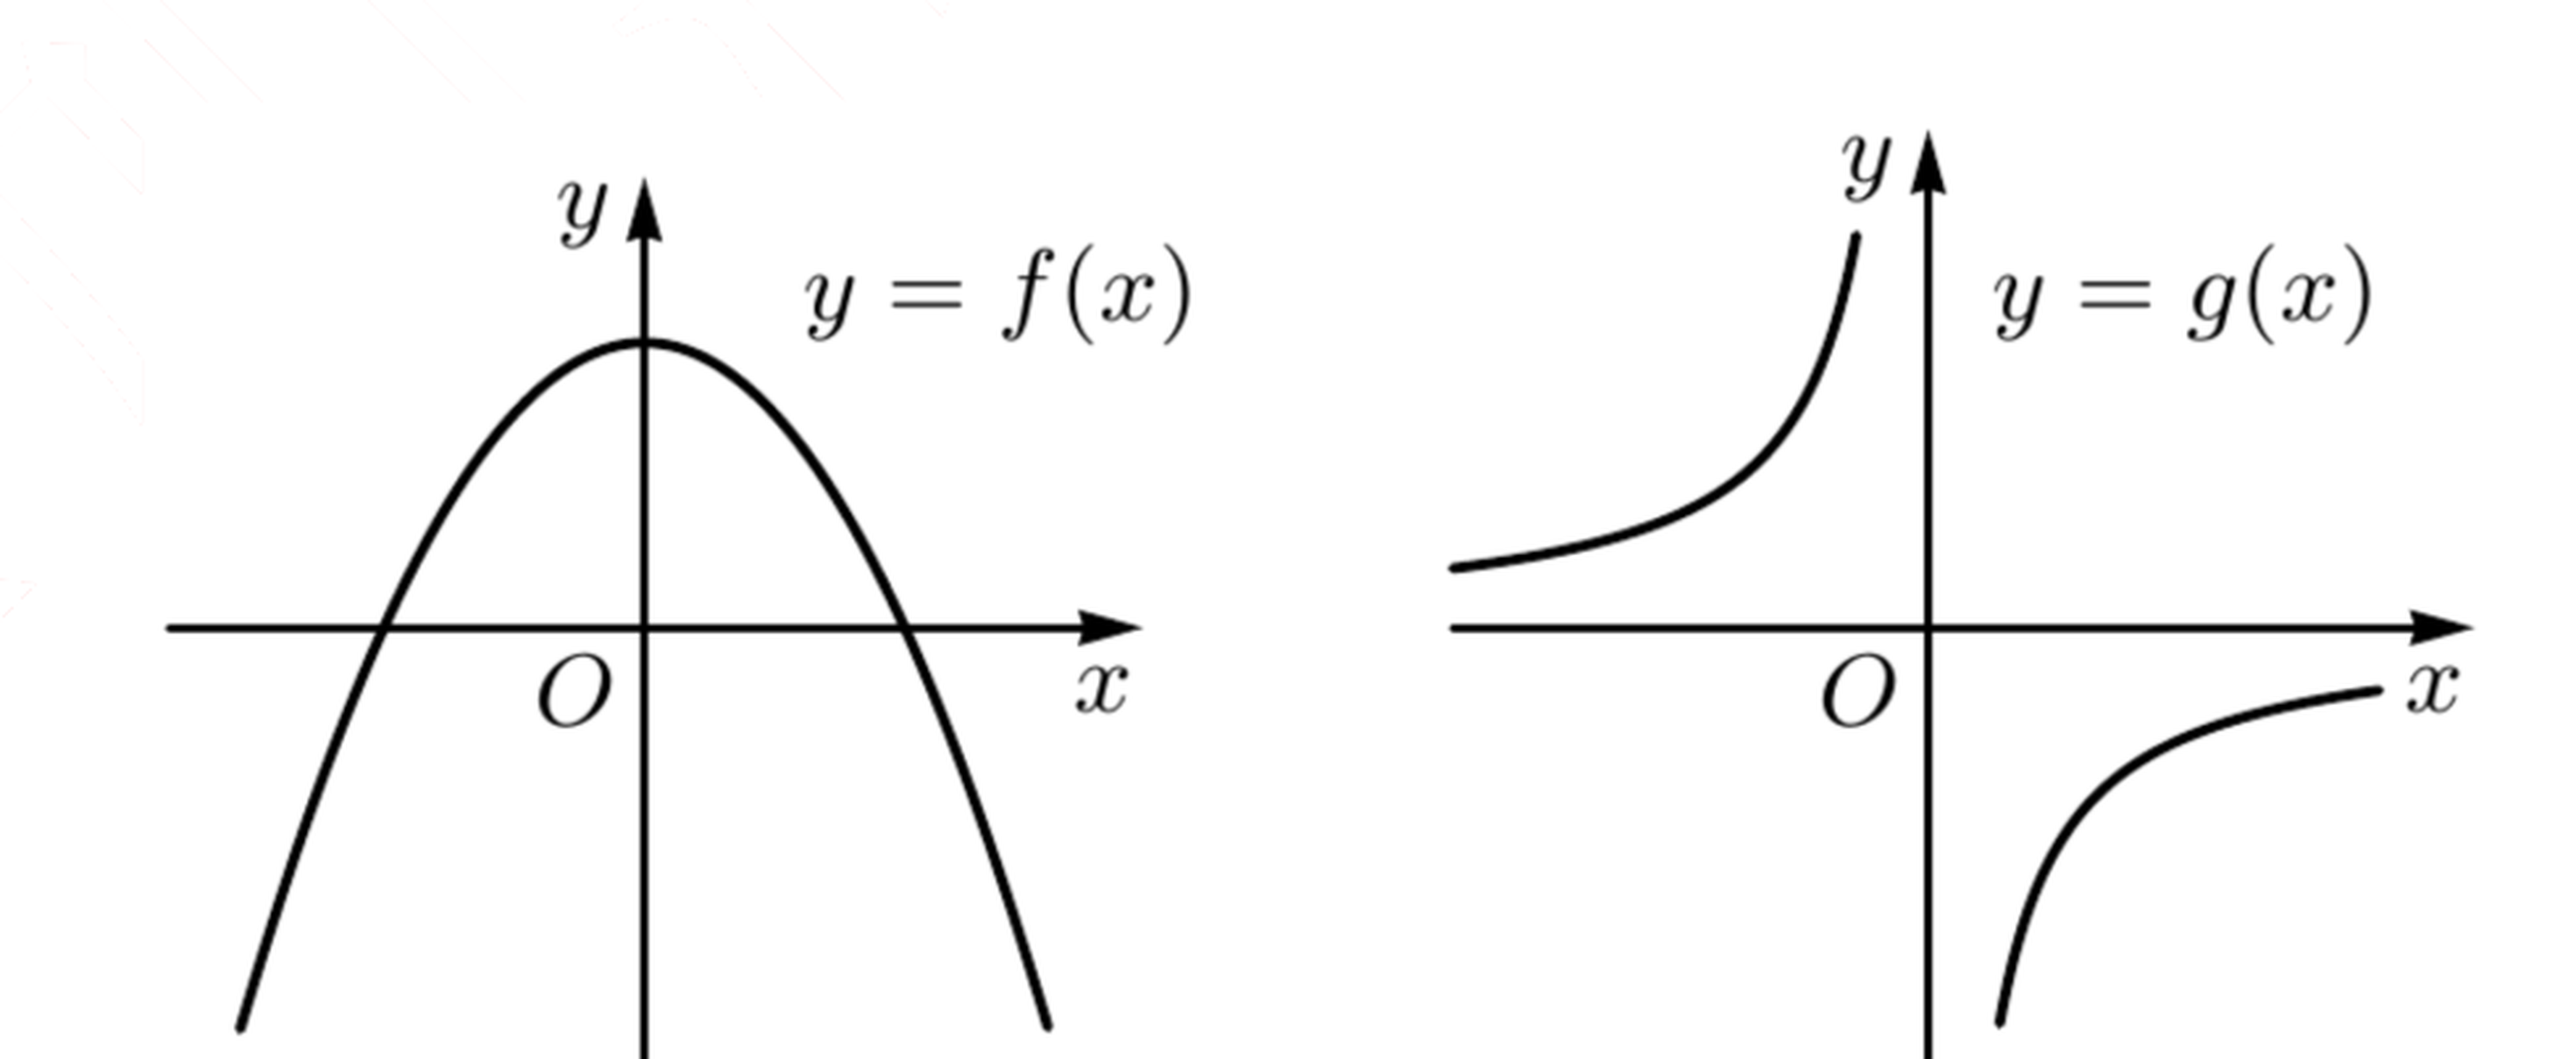
\includegraphics[width=0.72\textwidth]{figures/gao134_q13_graphs.png}\\[0.6em]
% A/B/C/D 四幅函数图象选项取原卷 04 页截图去粉色水印，按原卷一行四幅排布合并为一张
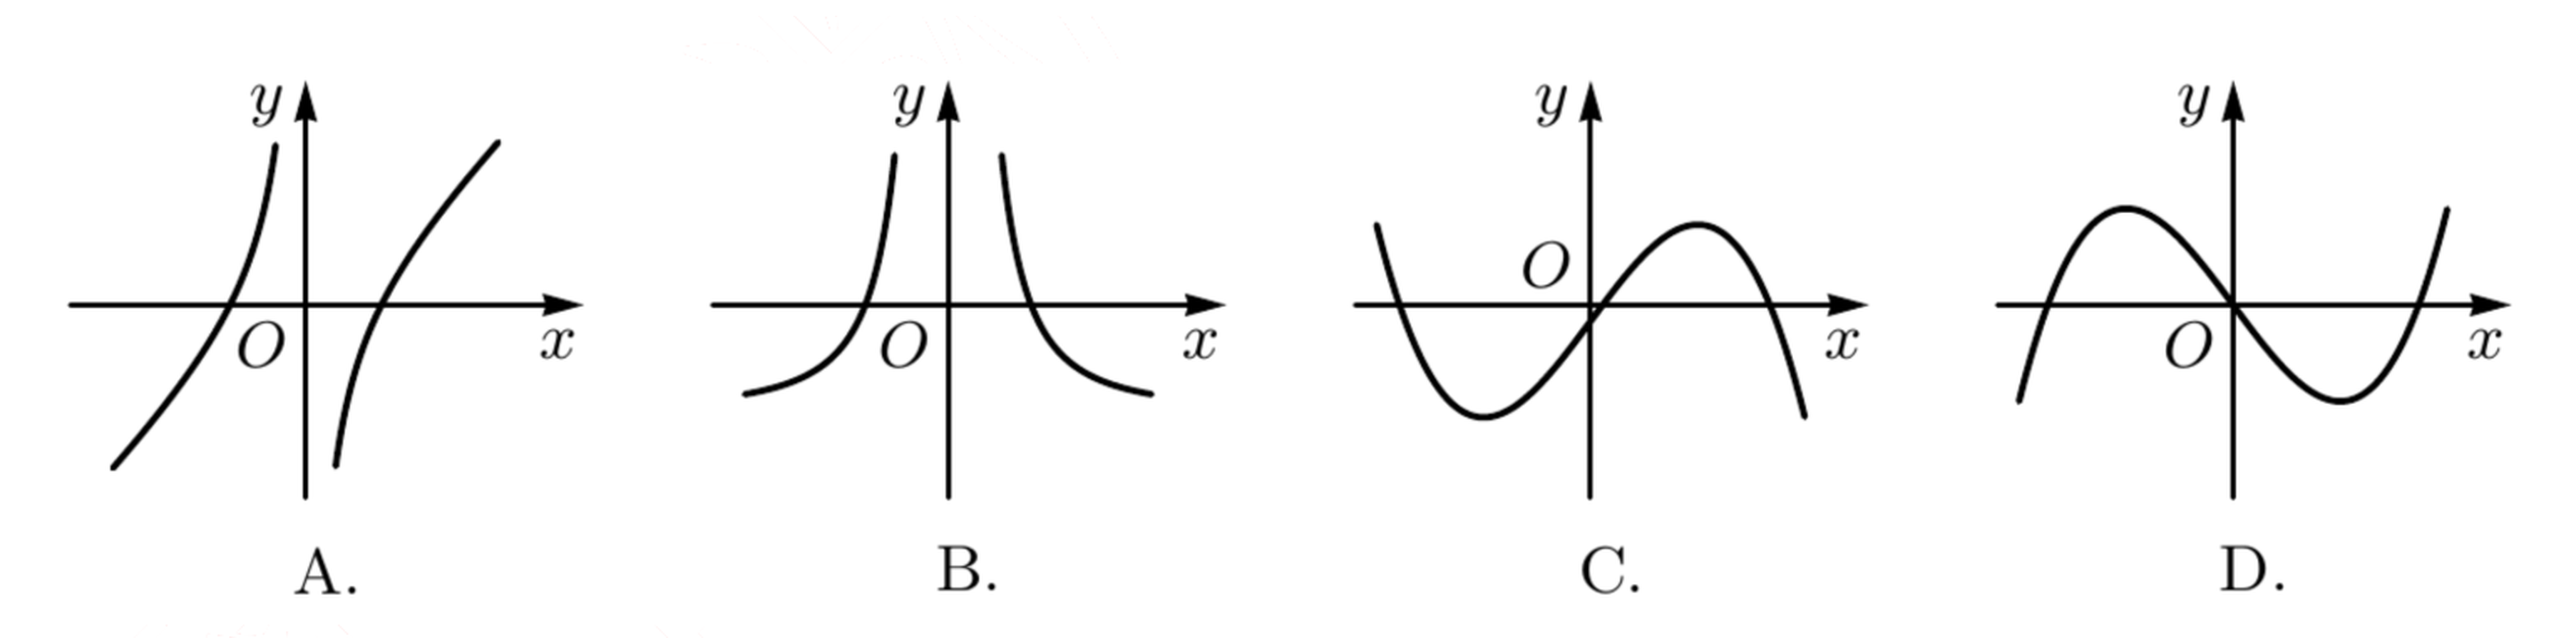
\includegraphics[width=0.90\textwidth]{figures/gao134_q13_options.png}
\end{center}

\ifanswer
\solbegin
\step{$f(x)$ 为偶函数，$g(x)$ 为奇函数，因此 $f(x)g(x)$ 为奇函数，排除 B.}
\step{又 $x=0$ 不在乘积函数的定义域内，其图象在 $y$ 轴上没有点，排除 C、D，}
\step{故选 $A$.}
\solend
\fi

\item 设全集为自然数集 $\N$，$E=\{x\mid x=2n,n\in\N\}$，$F=\{x\mid x=4n,n\in\N\}$，那么集合 $\N$ 可以表示成\mbox{（\quad）}

\keepwithprev
A. $E\cap F$\qquad\qquad B. $\overline{E}\cup F$\qquad\qquad C. $\overline{F}\cup E$\qquad\qquad D. $\overline{E}\cap\overline{F}$

\ifanswer
\solbegin
\step{$F\subseteq E$，所以 $\overline{F}\cup E=\N$，故选 $C$.}
\solend
\fi

\item 已知函数 $y=f(x)$，其中 $f(x)=x^2+bx$，则“$b<0$”是“$f(f(x))$ 的最小值与 $f(x)$ 的最小值相等”的\mbox{（\quad）}

\keepwithprev
A. 充分非必要条件\qquad\qquad B. 必要非充分条件

C. 充分必要条件\qquad\qquad D. 既非充分又非必要条件

\ifanswer
\solbegin
\step{$f(x)=\left(x+\dfrac b2\right)^2-\dfrac{b^2}4$，最小值为 $-\dfrac{b^2}4$，值域为 $\left[-\dfrac{b^2}4,+\infty\right)$.}
\step{当 $b<0$ 时，$-\dfrac b2>0\geqslant-\dfrac{b^2}4$，存在 $x$ 使 $f(x)=-\dfrac b2$，}
\step{从而 $f(f(x))$ 的最小值也为 $-\dfrac{b^2}4$，充分性成立.}
\step{当 $b=0$ 时，$f(x)=x^2$，$f(f(x))=x^4$，两者最小值均为 $0$，必要性不成立.}
\step{故选 $A$.}
\solend
\fi

\item 已知 $a,b,c\in\R$，若存在常数 $M>0$，使得 $a^2+b^2+c^2<M$，则称 $(a,b,c)$ 是有界数组. 对以下两个命题：

①若 $\lvert a^2+b+c\rvert+\lvert a^2+b-c\rvert\leqslant1$，则 $(a,b,c)$ 是有界数组；

②若 $\lvert a^2+b+c\rvert+\lvert a+b^2-c\rvert\leqslant1$，则 $(a,b,c)$ 是有界数组.% ②第二项为 \lvert a+b^2-c\rvert，与①刻意不同，照录

下列判断正确的是\mbox{（\quad）}

\keepwithprev
A. ①和②均为真命题\qquad\qquad B. ①和②均为假命题

C. ①为真命题，②为假命题\qquad D. ①为假命题，②为真命题

\ifanswer
\solbegin
\step{①取 $a=t,b=-t^2,c=0$，条件左端为 $0$，而 $a^2+b^2+c^2=t^2+t^4$ 可任意大，}
\step{故①为假命题.}
\step{②由条件，$a^2+a+b^2+b\leqslant\lvert a^2+b+c\rvert+\lvert a+b^2-c\rvert\leqslant1$.}
\step{由 $(a+1)^2+(b+1)^2\geqslant0$，得 $a^2+b^2\leqslant2(a^2+a+b^2+b)+2\leqslant4$.}
\step{又 $\lvert c\rvert\leqslant\lvert a^2+b+c\rvert+a^2+\lvert b\rvert\leqslant1+4+2=7$，故 $a^2+b^2+c^2\leqslant53<54$，}
\step{可取 $M=54$，故②为真命题.}
\step{故选 $D$.}
\solend
\fi

\end{enumerate}

\bigsec{三、解答题}

\begin{enumerate}
\setcounter{enumi}{16}

\item 已知不等式 $x^2-ax-b<0$ 的解集为 $A$，不等式 $\dfrac{3-2x}{x-1}<0$ 的解集为 $B$.

(1) 若 $a=5$，$b=-6$，求 $A\cap\overline{B}$；

(2) 若 $b=2a^2$，且 $A\cup B=B$，求实数 $a$ 的取值范围.

\ifanswer
\solbegin
\step{(1) 不等式 $\dfrac{3-2x}{x-1}<0$ 等价于 $x<1$ 或 $x>\dfrac32$，}
\step{所以 $B=(-\infty,1)\cup\left(\dfrac32,+\infty\right)$，$\overline{B}=\left[1,\dfrac32\right]$，}
\step{由 $x^2-5x+6=(x-2)(x-3)<0$，得 $A=(2,3)$，因此 $A\cap\overline{B}=\varnothing$.}
\step{(2) $A\cup B=B\Leftrightarrow A\subseteq B$，且 $x^2-ax-2a^2=(x-2a)(x+a)$，}
\step{当 $a=0$ 时，$A=\varnothing$，满足条件.}
\step{当 $a>0$ 时，$A=(-a,2a)$，$-a<0<1$，$A\subseteq B\Leftrightarrow2a\leqslant1$，得 $0<a\leqslant\dfrac12$.}
\step{当 $a<0$ 时，$A=(2a,-a)$，$2a<0<1$，$A\subseteq B\Leftrightarrow-a\leqslant1$，}
\step{得 $-1\leqslant a<0$.}
\step{因此 $a$ 的取值范围为 $\left[-1,\dfrac12\right]$.}
\solend
\fi

\item 为了在夏季降温和冬季供暖时减少能源损耗，房屋的屋顶和外墙需要建造隔热层. 某幢建筑物要建造可使用 $30$ 年的隔热层，每厘米厚的隔热层建造成本为 $9$ 万元. 该建筑物每年的能源消耗费用 $C$（万元）与隔热层厚度 $x$（cm）满足如下关系式：$C=\dfrac{k}{3x+5}$（$0\leqslant x\leqslant10$）. 若不建隔热层，每年能源消耗费用为 $8$ 万元. 设 $y$（万元）为隔热层建造费用与 $30$ 年的能源消耗费用之和.

(1) 求 $k$ 的值及 $y$ 的表达式；

(2) 隔热层修建多厚时，总费用 $y$ 最小？并求最小值.

\ifanswer
\solbegin
\step{(1) 不建隔热层时 $x=0$，$C=8$，所以 $\dfrac k5=8$，得 $k=40$.}
\step{隔热层建造费用为 $9x$ 万元，$30$ 年的能源消耗费用为 $30\times\dfrac{40}{3x+5}$ 万元.}
\step{因此 $y=9x+\dfrac{1200}{3x+5}$，$0\leqslant x\leqslant10$.}
\step{(2) 令 $t=3x+5$，则 $5\leqslant t\leqslant35$，且 $y=3t+\dfrac{1200}{t}-15$，}
\step{因为 $t>0$，由基本不等式得 $y\geqslant2\sqrt{3t\cdot\dfrac{1200}{t}}-15=105$，}
\step{当且仅当 $3t=\dfrac{1200}{t}$，即 $t=20$时取等号，此时 $x=5\in[0,10]$，}% 原卷"20"与"时"之间未留空，照录
\step{所以隔热层厚度为 $5$ cm 时，总费用最小，最小值为 $105$ 万元.}
\solend
\fi

\item 已知 $f(x)=ax^2+\dfrac1x$，其中 $a$ 为常数.

(1) 若 $a\in(1,3)$，判断函数 $y=f(x)$ 在 $[1,2]$ 上的单调性，并用定义证明；

(2) 求函数 $y=f(x)-x-\dfrac1x$ 在 $[1,2]$ 上的最大值 $g(a)$.

\ifanswer
\solbegin
\step{(1) 任取 $x_1,x_2\in[1,2]$，且 $x_1<x_2$，}
\step{则 $f(x_2)-f(x_1)=(x_2-x_1)\left[a(x_1+x_2)-\dfrac1{x_1x_2}\right]$，}
\step{由 $a>1$，$x_1+x_2\geqslant2$，$x_1x_2\geqslant1$，得 $a(x_1+x_2)-\dfrac1{x_1x_2}>2-1>0$，}
\step{因此 $f(x_2)>f(x_1)$，$f(x)$ 在 $[1,2]$ 上为严格增函数.}
\step{(2) 令 $h(x)=f(x)-x-\dfrac1x=ax^2-x$，其中 $x\in[1,2]$.}
\step{若 $a=0$，则 $h(x)=-x$，所以 $h(x)_{max}=h(1)=-1$；}
\step{若 $a<0$，二次函数的图象的对称轴为 $x=\dfrac1{2a}<0$，}
\step{所以 $y=h(x)$ 在 $[1,2]$ 上是严格减函数，所以 $h(x)_{max}=h(1)=a-1$；}
\step{若 $a>0$ 且 $\dfrac1{2a}>\dfrac32$，即 $0<a<\dfrac13$ 时，$h(x)_{max}=h(1)=a-1$.}
\step{若 $a>0$ 且 $\dfrac1{2a}\leqslant\dfrac32$，即 $a\geqslant\dfrac13$ 时，$h(x)_{max}=h(2)=4a-2$.}
\step{综上所述，$g(a)=\begin{cases}a-1,a<\dfrac13\\4a-2,a\geqslant\dfrac13\end{cases}$.}
\solend
\fi

\item 已知 $f(x)=\dfrac{ax^2+1}{bx+c}$（$a,b,c\in\Z$）.

(1) 若函数 $y=f(x)$ 是奇函数，且 $f(1)=2$，$f(2)<3$，求 $a,b,c$ 的值；

(2) 若函数 $y=f(x)$ 是偶函数，且 $ac<0$，$f(2a^2+a+1)<f(-3a^2+2a-1)$，求 $a$ 的值；

(3) 若 $b=a+c^2$，且满足不等式 $\lvert f(x)\rvert\geqslant1$ 的 $x$ 的最大值为 $0$，求 $c$ 的值.

\ifanswer
\solbegin
\step{(1) 由 $f(-x)=-f(x)$，交叉相乘得 $2c(ax^2+1)=0$ 恒成立，}
\step{因此 $c=0$，$b\neq0$.}
\step{由 $f(1)=2$，得 $a+1=2b$，}
\step{于是 $f(2)=\dfrac{4a+1}{2b}=4-\dfrac3{2b}<3\Leftrightarrow0<b<\dfrac32$，}
\step{因为 $b\in\Z$，所以 $b=1$，进而 $a=1$，$c=0$.}
\step{(2) 由 $f(-x)=f(x)$，交叉相乘得 $2bx(ax^2+1)=0$ 恒成立，因此 $b=0$.}
\step{此时 $f(x)=\dfrac ac x^2+\dfrac1c$，且 $\dfrac ac<0$.}
\step{设 $u=2a^2+a+1$，$v=-3a^2+2a-1$.}
\step{方程 $2a^2+a+1=0$ 与 $3a^2-2a+1=0$ 的判别式分别为 $-7$ 与 $-8$，}
\step{都小于 $0$，所以 $u>0$，$v<0$.}
\step{于是 $f(u)<f(v)\Leftrightarrow u^2>v^2\Leftrightarrow u>-v\Leftrightarrow-a^2+3a>0\Leftrightarrow0<a<3$，}
\step{因为 $a\in\Z$，所以 $a=1$ 或 $a=2$.}
\step{(3) 因为解集的最大值为 $0$，所以 $f(0)$ 有定义且 $\lvert f(0)\rvert\geqslant1$，}
\step{即 $c\neq0$，$\left\lvert\dfrac1c\right\rvert\geqslant1$，结合 $c\in\Z$，得 $c=\pm1$，从而 $b=a+1$.}
\step{当 $x=2$ 时，分母 $2a+2+c$ 为奇数，必不为 $0$；}
\step{又因为 $2>0$，必须有 $\lvert f(2)\rvert<1\Leftrightarrow\lvert4a+1\rvert<\lvert2a+2+c\rvert$，}
\step{若 $c=-1$，则 $(4a+1)^2<(2a+1)^2\Leftrightarrow4a(3a+1)<0\Leftrightarrow-\dfrac13<a<0$，}
\step{不存在满足条件的整数 $a$.}
\step{若 $c=1$，则 $(4a+1)^2<(2a+3)^2\Leftrightarrow4(3a+2)(a-1)<0\Leftrightarrow-\dfrac23<a<1$，}
\step{所以 $a=0$，$b=1$，此时 $f(x)=\dfrac1{x+1}$，}
\step{且 $\lvert f(x)\rvert\geqslant1\Leftrightarrow0<\lvert x+1\rvert\leqslant1\Leftrightarrow x\in[-2,-1)\cup(-1,0]$，}
\step{解集的最大值确为 $0$，因此 $c=1$.}
\solend
\fi

\item 已知函数 $y=f(x)$ 的定义域为 $\R$，且当 $x>0$ 时，$f(x)=\dfrac1{x+1}$. 对任意 $x_0\in\R$，定义集合 $D(x_0)=\{d\mid f(x_0+d)>f(x_0)\}$.

(1) 若当 $x\leqslant0$ 时，$f(x)=-2x+1$，求函数 $y=f(x)$ 的值域；

(2) 若 $y=f(x)$ 是偶函数，且 $f(0)=1$，求证：$D(-2)=\{-d\mid d\in D(2)\}$；

(3) 若 $y=f(x)$ 是奇函数，且 $x_1x_2\neq0$，求证：“$f(x_1)\leqslant f(x_2)$”的充要条件是\!\mbox{“$D(x_2)\subseteq D(x_1)$”}.

\ifanswer
\solbegin
\step{(1) 当 $x>0$ 时，$0<f(x)<1$；当 $x\leqslant0$ 时，$f(x)=-2x+1\geqslant1$.}
\step{函数的值域为 $(0,1)\cup[1,+\infty)=(0,+\infty)$.}
\step{(2) 由 $f(x)$ 是偶函数及 $f(0)=1$，得 $f(x)=\dfrac1{1+\lvert x\rvert}$，且 $f(2)=f(-2)=\dfrac13$.}
\stepm{法一：}{$D(2)=\left\{d\mid\dfrac1{1+\lvert2+d\rvert}>\dfrac13\right\}=\{d\mid\lvert2+d\rvert<2\}=(-4,0)$，}
\step{$D(-2)=\left\{d\mid\dfrac1{1+\lvert-2+d\rvert}>\dfrac13\right\}=\{d\mid\lvert-2+d\rvert<2\}=(0,4)$，}
\step{因此 $\{-d\mid d\in D(2)\}=(0,4)=D(-2)$.}
\stepm{法二：}{任取 $d\in D(-2)$，由定义得 $f(-2+d)>f(-2)$.}
\step{因为 $y=f(x)$ 是偶函数，所以对任意的实数 $x$，有 $f(-x)=f(x)$，}
\step{因此 $f(-2+d)=f(-(-2+d))=f(2-d)$，且 $f(-2)=f(2)$.}
\step{所以不等式 $f(-2+d)>f(-2)$ 等价于 $f(2-d)>f(2)$，}
\step{这恰好是 $-d\in D(2)$ 的定义，}
\step{所以 $d\in D(-2)\Leftrightarrow-d\in D(2)$，故 $D(-2)=\{-d\mid d\in D(2)\}$.}
\step{(3) 由 $f(x)$ 是奇函数，得 $f(0)=0$；}
\step{当 $x<0$ 时，$f(x)=-f(-x)=-\dfrac1{1-x}=\dfrac1{x-1}$；}
\step{所以 $f(x)=\begin{cases}\dfrac1{x-1},&x<0\\0,&x=0;\\\dfrac1{x+1},&x>0\end{cases}$}
% 2026-11-15 回原图订正：原卷 11 页此 cases 块末无句点，本稿初转顺手补了西文句点，今删去（Q19 08 页同类块末有句点，照录保留）。
\step{当 $x_0<0$ 时，$D(x_0)=\{d\mid f(x_0+d)>f(x_0)\}=(-\infty,0)\cup[-x_0,+\infty)$，}
\step{当 $x_0=0$ 时，$D(0)=\{d\mid f(0+d)>f(0)\}=(0,+\infty)$，}
\step{当 $x_0>0$ 时，$D(x_0)=\{d\mid f(x_0+d)>f(x_0)\}=(-x_0,0)$.}
\stepm{先证明必要性.}{若 $f(x_1)\leqslant f(x_2)$，仅需讨论三类情形：}
\step{若 $x_2\leqslant x_1<0$，}
\step{则 $D(x_1)=(-\infty,0)\cup[-x_1,+\infty),D(x_2)=(-\infty,0)\cup[-x_2,+\infty)$，}
\step{故 $D(x_2)\subseteq D(x_1)$；}
\step{若 $0<x_2\leqslant x_1$，则 $D(x_1)=(-x_1,0),D(x_2)=(-x_2,0)$，}
\step{故 $D(x_2)\subseteq D(x_1)$；}
\step{若 $x_1<0<x_2$，则 $D(x_1)=(-\infty,0)\cup[-x_1,+\infty),D(x_2)=(-x_2,0)$，}
\step{故 $D(x_2)\subseteq D(x_1)$.}
\stepm{再证明充分性.}{若 $D(x_2)\subseteq D(x_1)$，}
\step{若 $x_1<0,x_2<0$，}
\step{则 $D(x_1)=(-\infty,0)\cup[-x_1,+\infty),D(x_2)=(-\infty,0)\cup[-x_2,+\infty)$，}
\step{由 $D(x_2)\subseteq D(x_1)$ 得 $x_2\leqslant x_1$，}
\step{又 $y=f(x)$ 在 $(-\infty,0)$ 上是严格减函数，所以 $f(x_1)\leqslant f(x_2)$；}
\step{若 $x_1>0,x_2>0$，则 $D(x_1)=(-x_1,0),D(x_2)=(-x_2,0)$，}
\step{由 $D(x_2)\subseteq D(x_1)$ 得 $x_2\leqslant x_1$，}
\step{又 $y=f(x)$ 在 $(0,+\infty)$ 上是严格减函数，所以 $f(x_1)\leqslant f(x_2)$；}
\step{若 $x_1<0,x_2>0$，则 $f(x_1)<0<f(x_2)$，结论成立；}
\step{若 $x_1>0,x_2<0$，此时 $D(x_1)=(-x_1,0)$ 中只有负数，}
\step{而 $D(x_2)=(-\infty,0)\cup[-x_2,+\infty)$ 中有正数，$D(x_2)\subseteq D(x_1)$ 不成立.}
\step{综上，“$f(x_1)\leqslant f(x_2)$”的充要条件是“$D(x_2)\subseteq D(x_1)$”.}
\solend
\fi

\end{enumerate}

\end{document}
"
%
% ① 原始材料：微信公众号"魔都数学加油站"文章，作者破晓，2026-11-15 18:04 发布；
% 连载"27学年高一134"，原文标题"27学年高一134——2026-2027年上海市华师大二附中高一上期中"；
% 原文链接：https://mp.weixin.qq.com/s/bQlkmlGdCtAlytY331vf3g。
% 正文为 13 张 PNG 页（01、04、06、08、09、10、11、12、13 为 2560x3620；
% 02、03、05、07 为 4762x6735，同一篇各页分辨率不同，逐页按各自分辨率裁图核对），
% 题目下印有【解析】，为讲评版。题目、解析均据原图转录；卷面粉红色水印
% "魔都数学加油站"及公众号页脚未录入。
% 全卷 2 幅插图，均在第 04 页：第 13 题题干 y=f(x)、y=g(x) 两幅函数图象合并裁为
% figures/gao134_q13_graphs.png，第 13 题 A/B/C/D 四幅函数图象选项合并裁为
% figures/gao134_q13_options.png；两图均取原卷 04 页截图 3× LANCZOS 放大、
% 白化粉色水印（只白化浅粉色 R>175 且 G>140 且 B>140 的像素，保留红色标签）。
% 注意：本卷 Q13 四幅选项在原卷排为"一行四幅"（1×4），并非 高一132 第 14 题
% 的 2×2 排布，本稿按原卷 1×4 合并裁为一张，不重排、不用 TikZ 重绘。
%
% 卷首标题：原卷印作"2026-2027 年华师大二附中高一上期中"（公众号标题中的"上海市"
% 卷面标题行没有，本稿照卷面），年份区间按全稿惯例排 en dash；原卷未印副标题，
% 本卷为期中卷、跨集合与常用逻辑用语／不等式／函数三章，按题目内容标为
% "集合与常用逻辑用语、不等式、函数"（与 125／126／128／129／131／132／133 同期中卷口径相同）：
% 集合与逻辑见 Q6、Q10、Q14、Q16、Q17、Q21，不等式见 Q3、Q7、Q9、Q11、Q15、Q18、Q19，
% 函数（函数性质、二分法、奇偶性、基本不等式应用）见 Q4、Q5、Q8、Q12、Q13、Q20。
%
% 题号体例：本卷共 19 题——一、填空题 3—12（10 题）、二、选择题 13—16（4 题）、
% 三、解答题 17—21（5 题）。三节分别 \setcounter{enumi}{2}／{12}／{16}。
% 第 13 页仅为 Q21 (3) 解析续尾，全卷无「四、附加题」。
%
% ② 与原卷的排版差异：
%   ① 原文从第 3 题起，本稿保留原题号（见上"题号体例"）；
%   ② 原卷每题下直接印【解析】，本稿按全稿惯例置于答案版；第 13—16 题答案均在
%      解析末句"故选 …"，题干括号内留空、不另提 \ans{}（四题均无独立答案段）；
%      全卷无只印括号内答案、无解析的选择题；
%   ③ 原卷未印副标题，本稿按"知识模块"口径补出；
%   ④ 原卷填空横线按全稿惯例排为 \blankline[4.4em]；选择题括号排 \mbox{（\quad）}、
%      每个选项段前按惯例加 \keepwithprev（Q13 四选项为图，守卫前行为 \begin{center}；
%      Q15、Q16 四选项分两行排，\keepwithprev 只加在 A. 行前）；解答题不留作答区、
%      不加 \anspace（原卷为讲评版，与 129／131／132／133 同）；
%   ⑤ 原卷数集印黑板粗体（Q7／Q11／Q12／Q16／Q21 的 R、Q14／Q20 的 N、Q20 的 Z），
%      按全稿惯例统一排 \R／\N／\Z；绝对值排 \lvert…\rvert，集合描述竖线排 \mid；不等号按全稿惯例排
%      \leqslant／\geqslant；补集照原卷上划线排 \overline{B}、\overline{E}、\overline{F}；
%   ⑥ 子题标号 (1)(2)(3) 与括注原卷均用半角括号，照录（与 131／132／133 同）；
%      圈数字 ①② 照录；原卷 Q21 (2) 解析"法一：""法二："与 Q21 (3) 解析
%      "先证明必要性.""再证明充分性."四处标签印红色加粗，按 高一53／108／133 成例排
%      \stepm{法一：}／\stepm{法二：}／\stepm{先证明必要性.}／\stepm{再证明充分性.}
%      （加粗着色、不引入红色，不动 common.sty）；Q8 解析"第 1 步：""第 2 步：""
%      "第 3 步："原卷印黑色常规宋体（非红非粗），照录为普通 \step 行内文字；
%   ⑦ 数学式内半角逗号照录（如 Q6 $A=\{0,1,2,3\}$、Q14 $x=2n,n\in\N$、
%      Q16 $a,b,c\in\R$ 与 $a=t,b=-t^2,c=0$、Q19 $x_1,x_2\in[1,2]$、
%      Q20 $a,b,c\in\Z$、Q21 $x_1<0,x_2<0$ 与 $D(x_1)=(-x_1,0),D(x_2)=(-x_2,0)$）；
%      原卷行末全角句点按全稿惯例从宽排西文句点；cases 块末的句点逐处照录：
%      Q19 解析（08 页）块末原卷有句点照录、Q21 (3) 解析（11 页）块末原卷无句点不补，
%      两处原卷自身不统一（2026-11-15 回原图核对，本稿初转曾顺手补句点，已删去）；
%   ⑧ 原卷 Q8 解析跨 01—02 页、Q10 解析跨 02—03 页、Q12 解析跨 03—04 页、
%      Q16 解析跨 05—06 页、Q17 解析跨 06—07 页、Q20 解析跨 08—10 页、
%      Q21 解析跨 10—13 页，本稿按题合并连续排版；末页第 13 页为
%      Q21 (3) 解析续尾与"综上"一句，按实际印刷行单列；
%   ⑨ 题干中的中文弯引号按原卷照录（Q10 研究问题、Q15 条件、Q21 (3) 充要条件），
%      注释内一律 ASCII 引号。
%
% 判别式字形：全卷仅 Q9 解析末行出现一处判别式记号
%   "两值均满足 $\Delta=p^2-4p=18\mp12\sqrt2>0$"，逐处放大核对，原卷印高三角
%   $\Delta$（等腰、高，实测高宽比约 1.14），照录 \Delta；卷内无扁三角 \triangle，
%   与 高一132 同题排 $\triangle$、高一133 部分判别式排 $\triangle$ 均不同。
%
% 子集符号：Q6 题干 $C\subseteq A$、$C\subseteq B$ 与解析 $C\subseteq A\cap B$、
%   Q14 解析 $F\subseteq E$、Q17 解析 $A\subseteq B$、Q21 题干与解析各处的
%   $D(x_2)\subseteq D(x_1)$，全部印带下划线的 $\subseteq$，逐处放大核对，
%   照录 \subseteq；全卷未出现单线 \subset。
%
% 原卷存疑照录（均照录未改，正文对应处另有 % 注）：
%   第 6 题题干集合 $A=\{0,1,2,3\}$ 三个逗号后不留空，紧邻的 $B=\{0,2,4,5\}$
%      三个逗号后却留空，同卷同一行两集合排字不一，照录其逗号均为半角；
%   第 16 题命题②作 $\lvert a^2+b+c\rvert+\lvert a+b^2-c\rvert\leqslant1$，
%      与命题①第二项 $\lvert a^2+b-c\rvert$ 不同（①无 $b$ 的平方、②有），
%      两命题刻意不同，照录；解析"②由条件，$a^2+a+b^2+b\leqslant\cdots$"
%      由两项相加直接得到，照录；
%   第 18 题 (2) 解析"即 $t=20$时取等号"中"20"与"时"之间原卷未留空，照录；
%   第 19 题解析 $h(x)_{max}$ 的"max"下标三处字形不一（斜体／正体混排），照录；
%   第 20 题 (1)(2) 解析"由 $f(-x)=-f(x)$，交叉相乘得……"与"由 $f(-x)=f(x)$，
%      交叉相乘得……"两处措辞照录；
%   第 21 题 (2) 原卷并存"法一"（集合计算）与"法二"（定义推证）两套证明，照录不删。
%
% 行数复核：逐题数 \step/\stepm 条数，合计 134 条（Q3：2；Q4：1；Q5：1；Q6：1；
% Q7：2；Q8：4；Q9：3；Q10：4；Q11：5；Q12：8；Q13：3；Q14：1；Q15：5；
% Q16：7；Q17：9；Q18：7；Q19：11；Q20：22；Q21：38），与原卷印刷行逐题相等
% （cases 块作一个印刷行计）。第 13—16 题答案在解析末句，括号内留空、不另提 \ans{}；
% 第 21 题四条 \stepm 计入 38 条内。
%
\documentclass[a4paper,11pt]{article}
\usepackage{common}

\begin{document}

\examtitlest[3]{2026--2027 年华师大二附中高一上期中}{集合与常用逻辑用语、不等式、函数}

\bigsec{一、填空题}

\begin{enumerate}
\setcounter{enumi}{2}

\item 不等式 $\lvert 2x+1\rvert\geqslant3$ 的解集为\blankline[4.4em].

\ifanswer
\solbegin
\step{$\lvert 2x+1\rvert\geqslant3\Leftrightarrow 2x+1\leqslant-3$ 或 $2x+1\geqslant3\Leftrightarrow x\leqslant-2$ 或 $x\geqslant1$，}
\step{故解集为 $(-\infty,-2]\cup[1,+\infty)$.}
\solend
\fi

\item 函数 $y=\sqrt{x+1}+\dfrac1x$ 的定义域为\blankline[4.4em].

\ifanswer
\solbegin
\step{$x+1\geqslant0$ 且 $x\neq0$，得定义域为 $[-1,0)\cup(0,+\infty)$.}
\solend
\fi

\item 已知等式 $3x^2-4x-2=a(x-1)^2+b(x-1)+c$ 恒成立，其中 $a$、$b$、$c$ 为常数，则 $a-b+c=$\blankline[4.4em].

\ifanswer
\solbegin
\step{令 $x=0$，得 $a-b+c=-2$.}
\solend
\fi

\item 已知集合 $A=\{0,1,2,3\}$，$B=\{0,2,4,5\}$，$C\subseteq A$，$C\subseteq B$，符合条件的集合 $C$ 有\blankline[4.4em]个.% 原卷 A 的逗号后不留空、B 的逗号后留空，排字不一，照录

\ifanswer
\solbegin
\step{$C\subseteq A\cap B=\{0,2\}$，所以符合条件的集合 $C$ 有 $2^2=4$ 个.}
\solend
\fi

\item 设 $a$、$b\in\R$，且 $a^2+4b^2=2$，则 $ab$ 的最大值为\blankline[4.4em].

\ifanswer
\solbegin
\step{$(a-2b)^2=a^2+4b^2-4ab=2-4ab\geqslant0$，得 $ab\leqslant\dfrac12$，}
\step{当且仅当 $a=2b=\pm1$ 时取等号，故 $ab$ 的最大值为 $\dfrac12$.}
\solend
\fi

\item 已知函数 $y=x(13-2x)^2-140$，用二分法求函数在区间 $(3,4)$ 上的零点时，第 3 步应计算 $x=$\blankline[4.4em]的函数值.

\ifanswer
\solbegin
\step{记 $f(x)=x(13-2x)^2-140$，则 $f(3)=7>0$，$f(4)=-40<0$.}
\step{第 1 步：$f\left(\dfrac72\right)=-14<0$，区间缩小为 $\left(3,\dfrac72\right)$.}
\step{第 2 步：$f\left(\dfrac{13}4\right)=-\dfrac{43}{16}<0$，区间缩小为 $\left(3,\dfrac{13}4\right)$.}
\step{第 3 步：应计算 $x=\dfrac{3+\frac{13}4}2=\dfrac{25}8$ 的函数值.}
\solend
\fi

\item 已知一元二次方程 $x^2+px+p=0$ 的两个实根分别为 $x_1$、$x_2$，且 $x_1^2x_2+x_2^2x_1=-18$，则 $p=$\blankline[4.4em].% 判别式 \Delta 高三角，逐处放大核对

\ifanswer
\solbegin
\step{由韦达定理，$x_1+x_2=-p$，$x_1x_2=p$，}
\step{则 $x_1^2x_2+x_2^2x_1=x_1x_2(x_1+x_2)=-p^2=-18\Rightarrow p=\pm3\sqrt2$，}
\step{两值均满足 $\Delta=p^2-4p=18\mp12\sqrt2>0$，故 $p=\pm3\sqrt2$.}
\solend
\fi

\item 研究问题：“已知关于 $x$ 的不等式 $ax^2-bx+c>0$ 的解集为 $(1,2)$，解关于 $x$ 的不等式 $cx^2-bx+a>0$”，有如下解法：

解：由 $ax^2-bx+c>0\Rightarrow a-b\left(\dfrac1x\right)+c\left(\dfrac1x\right)^2>0$，令 $y=\dfrac1x$，则 $y\in\left(\dfrac12,1\right)$，

所以不等式 $cx^2-bx+a>0$ 的解集为 $\left(\dfrac12,1\right)$.

参考上述解法，已知关于 $x$ 的不等式 $\dfrac{k}{x+a}+\dfrac{x+b}{x+c}<0$ 的解集为 $(-3,-1)\cup(2,4)$，则关于 $x$ 的不等式 $\dfrac{kx}{ax-1}+\dfrac{bx-1}{cx-1}<0$ 的解集为\blankline[4.4em].

\ifanswer
\solbegin
\step{当 $x=0$ 时，所求不等式左端为 $1$，不满足不等式.}
\step{当 $x\neq0$ 时，两个分式的分子、分母同除以 $x$，得 $\dfrac{k}{a-\frac1x}+\dfrac{b-\frac1x}{c-\frac1x}<0$.}
\step{令 $t=-\dfrac1x$，则所求不等式化为 $\dfrac{k}{t+a}+\dfrac{t+b}{t+c}<0$，即 $-\dfrac1x\in(-3,-1)\cup(2,4)$，}
\step{解得 $x\in\left(-\dfrac12,-\dfrac14\right)\cup\left(\dfrac13,1\right)$.}
\solend
\fi

\item 已知 $a\in(0,+\infty)$，若对任意的 $x\in(0,+\infty)$，均有 $\lvert x^2-a\rvert+\lvert x+b\rvert=\lvert x^2+x-a+b\rvert$，则 $a^2-b^2$ 的最小值为\blankline[4.4em].

\ifanswer
\solbegin
\step{原等式成立的充要条件是 $(x^2-a)(x+b)\geqslant0$.}
\step{当 $0<x<\sqrt a$ 时须有 $x+b\leqslant0$；当 $x>\sqrt a$ 时须有 $x+b\geqslant0$，因此 $b=-\sqrt a$.}
\step{此时 $(x^2-a)(x+b)=(x+\sqrt a)(x-\sqrt a)^2\geqslant0$，满足题意.}
\step{$a^2-b^2=a^2-a=\left(a-\dfrac12\right)^2-\dfrac14\geqslant-\dfrac14$，}
\step{当 $a=\dfrac12$，$b=-\dfrac{\sqrt2}2$ 时取等号，最小值为 $-\dfrac14$.}
\solend
\fi

\item 已知函数 $y=f(x)$ 在 $\R$ 上是严格增函数，当 $x\neq0$ 且 $f(x)\neq0$ 时，满足 $f(x)\cdot f\left[\dfrac1{f(x)}+\dfrac1x\right]=1$，则 $f(1)=$\blankline[4.4em].

\ifanswer
\solbegin
\step{当 $xf(x)>0$ 时，记 $t=\dfrac1{f(x)}+\dfrac1x\neq0$，则 $f(t)=\dfrac1{f(x)}\neq0$.}
\step{将 $t$ 代入题设，得 $f\left(f(x)+\dfrac1t\right)=f(x)$，严格增性给出 $f(x)+\dfrac1t=x$，}
\step{化简得 $f(x)^2+xf(x)-x^2=0$，由 $\dfrac{f(x)}x>0$ 得 $f(x)=\dfrac{\sqrt5-1}2x$.}
\step{设 $a=f(0)$，若 $a>0$，则 $f(a)>f(0)=a>0$；}
\step{若 $a<0$，则 $f(a)<f(0)=a<0$.}
\step{两种情形都有 $af(a)>0$ 且 $\dfrac{f(a)}a>1$，与上式 $\dfrac{f(a)}a=\dfrac{\sqrt5-1}2<1$ 矛盾，}
\step{因此 $f(0)=0$.}
\step{于是 $f(1)>0$，代入上式得 $f(1)=\dfrac{\sqrt5-1}2$.}
\solend
\fi

\end{enumerate}

% 第 13 题是"节标题 + 题干 + 两幅图 + 四幅选项图"约 15cm 的整块，
% 守卫只放在 \bigsec 之前；若再在 \item 之前放第二枚，会在标题已印出后才触发换页，
% 把题目推走、留下孤立节标题（切页审计 B 类）。高度须覆盖整块。
\needvspace{16cm}
\bigsec{二、选择题}

\begin{enumerate}
\setcounter{enumi}{12}

\item 已知函数 $y=f(x)$ 与 $y=g(x)$ 的图象如图所示，则函数 $y=f(x)\cdot g(x)$ 的图象可能是\mbox{（\quad）}

\keepwithprev
\begin{center}
% 题干 y=f(x)、y=g(x) 两幅函数图象取原卷 04 页截图去粉色水印，按原卷左右排布合并为一张
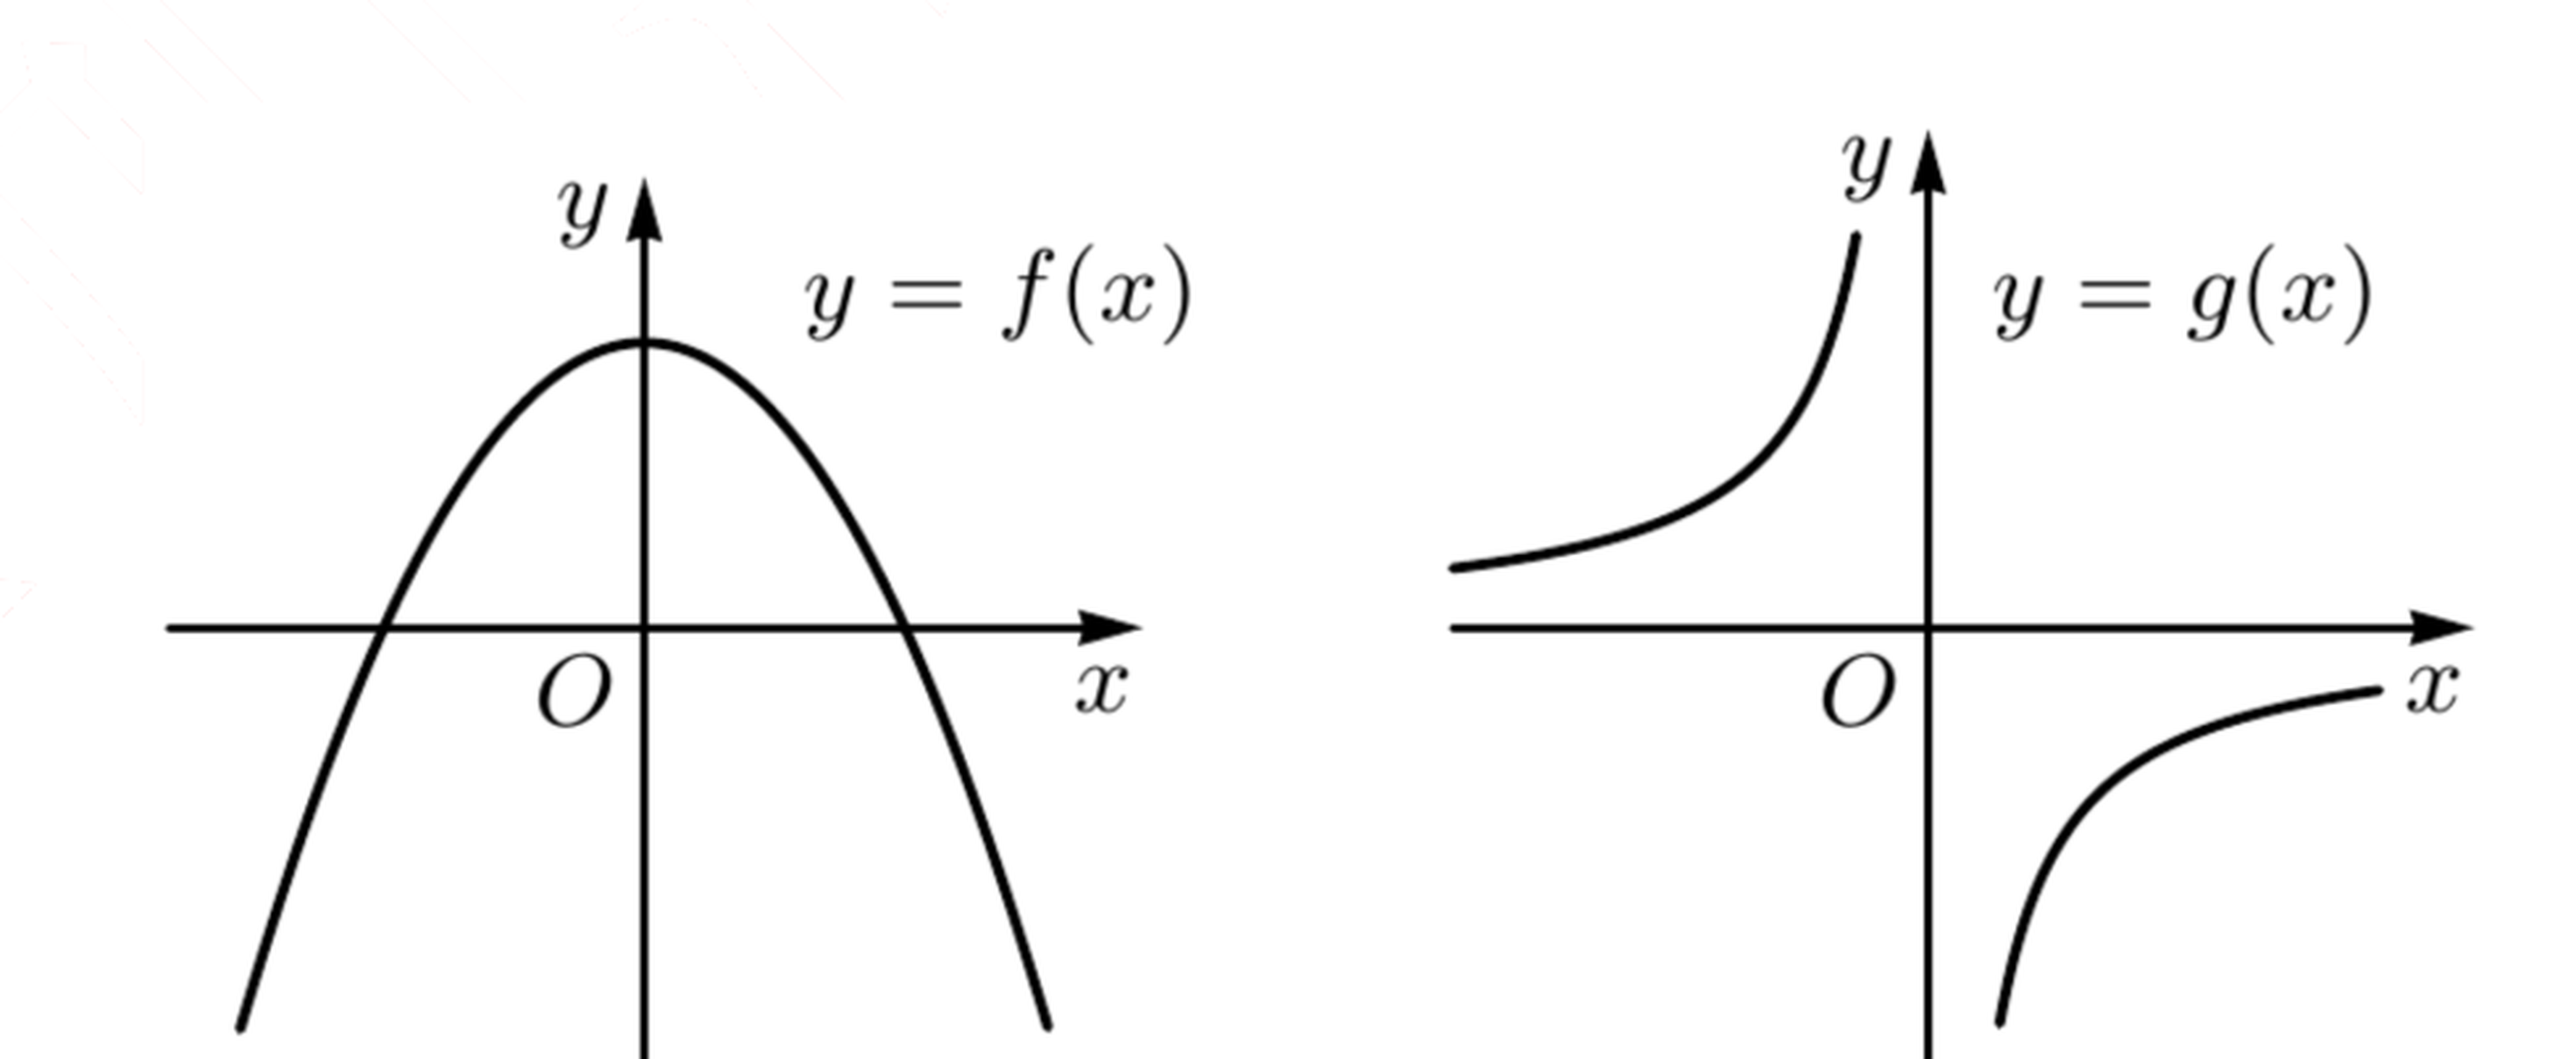
\includegraphics[width=0.72\textwidth]{figures/gao134_q13_graphs.png}\\[0.6em]
% A/B/C/D 四幅函数图象选项取原卷 04 页截图去粉色水印，按原卷一行四幅排布合并为一张
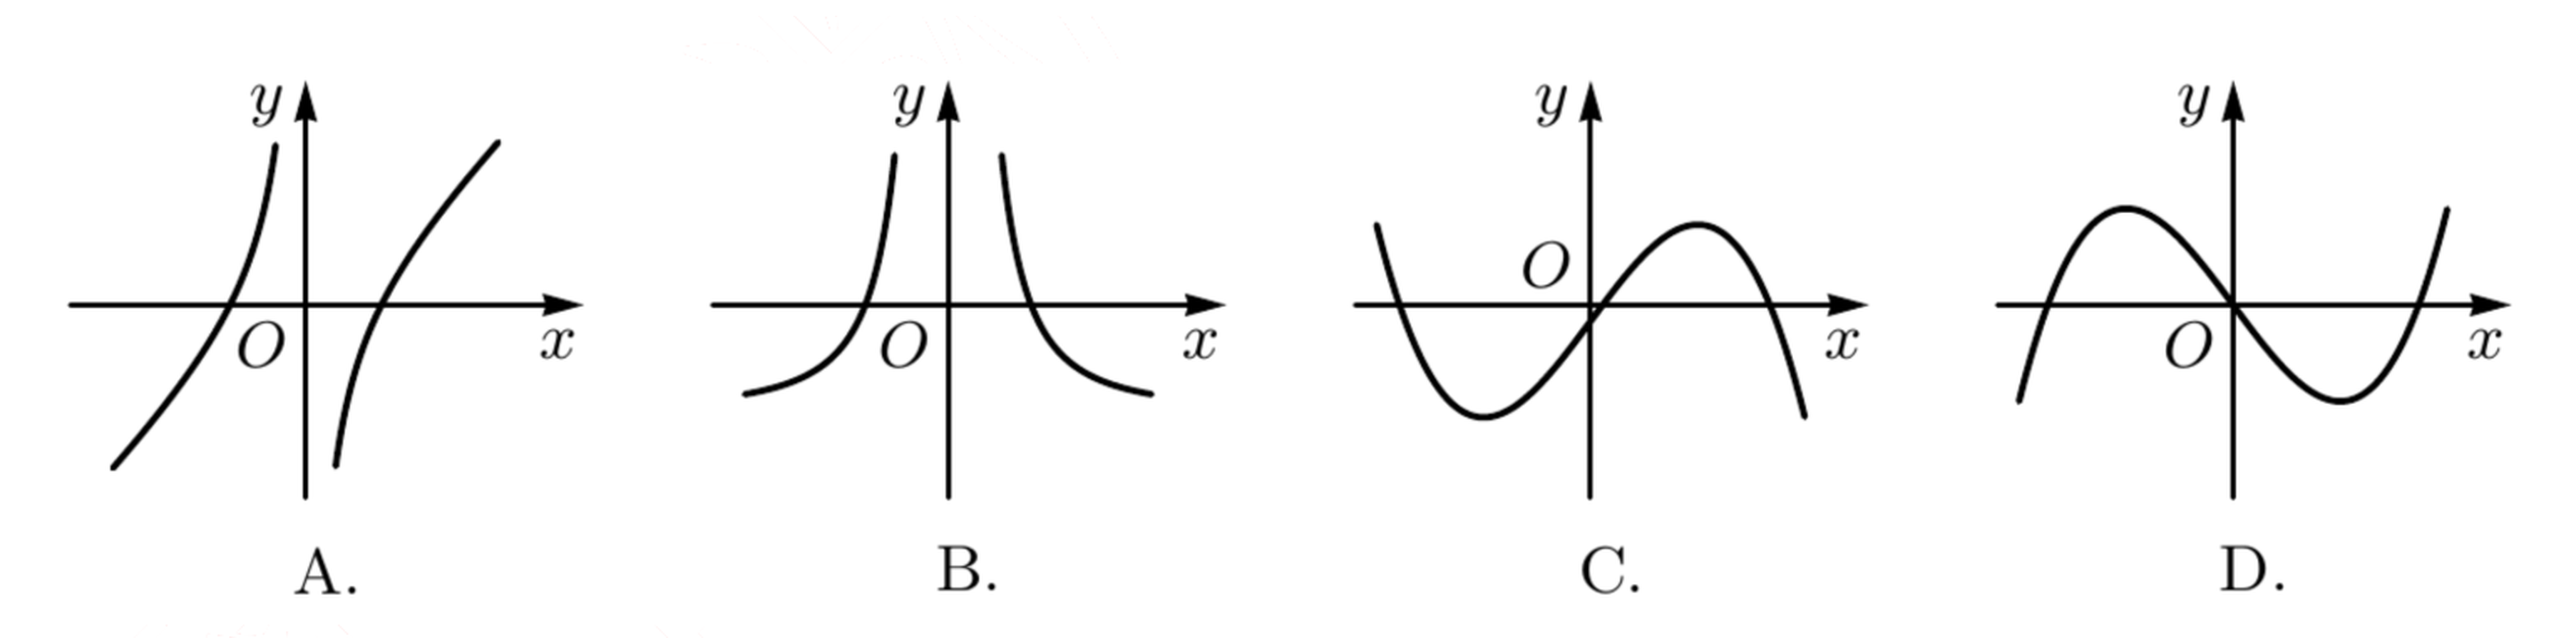
\includegraphics[width=0.90\textwidth]{figures/gao134_q13_options.png}
\end{center}

\ifanswer
\solbegin
\step{$f(x)$ 为偶函数，$g(x)$ 为奇函数，因此 $f(x)g(x)$ 为奇函数，排除 B.}
\step{又 $x=0$ 不在乘积函数的定义域内，其图象在 $y$ 轴上没有点，排除 C、D，}
\step{故选 $A$.}
\solend
\fi

\item 设全集为自然数集 $\N$，$E=\{x\mid x=2n,n\in\N\}$，$F=\{x\mid x=4n,n\in\N\}$，那么集合 $\N$ 可以表示成\mbox{（\quad）}

\keepwithprev
A. $E\cap F$\qquad\qquad B. $\overline{E}\cup F$\qquad\qquad C. $\overline{F}\cup E$\qquad\qquad D. $\overline{E}\cap\overline{F}$

\ifanswer
\solbegin
\step{$F\subseteq E$，所以 $\overline{F}\cup E=\N$，故选 $C$.}
\solend
\fi

\item 已知函数 $y=f(x)$，其中 $f(x)=x^2+bx$，则“$b<0$”是“$f(f(x))$ 的最小值与 $f(x)$ 的最小值相等”的\mbox{（\quad）}

\keepwithprev
A. 充分非必要条件\qquad\qquad B. 必要非充分条件

C. 充分必要条件\qquad\qquad D. 既非充分又非必要条件

\ifanswer
\solbegin
\step{$f(x)=\left(x+\dfrac b2\right)^2-\dfrac{b^2}4$，最小值为 $-\dfrac{b^2}4$，值域为 $\left[-\dfrac{b^2}4,+\infty\right)$.}
\step{当 $b<0$ 时，$-\dfrac b2>0\geqslant-\dfrac{b^2}4$，存在 $x$ 使 $f(x)=-\dfrac b2$，}
\step{从而 $f(f(x))$ 的最小值也为 $-\dfrac{b^2}4$，充分性成立.}
\step{当 $b=0$ 时，$f(x)=x^2$，$f(f(x))=x^4$，两者最小值均为 $0$，必要性不成立.}
\step{故选 $A$.}
\solend
\fi

\item 已知 $a,b,c\in\R$，若存在常数 $M>0$，使得 $a^2+b^2+c^2<M$，则称 $(a,b,c)$ 是有界数组. 对以下两个命题：

①若 $\lvert a^2+b+c\rvert+\lvert a^2+b-c\rvert\leqslant1$，则 $(a,b,c)$ 是有界数组；

②若 $\lvert a^2+b+c\rvert+\lvert a+b^2-c\rvert\leqslant1$，则 $(a,b,c)$ 是有界数组.% ②第二项为 \lvert a+b^2-c\rvert，与①刻意不同，照录

下列判断正确的是\mbox{（\quad）}

\keepwithprev
A. ①和②均为真命题\qquad\qquad B. ①和②均为假命题

C. ①为真命题，②为假命题\qquad D. ①为假命题，②为真命题

\ifanswer
\solbegin
\step{①取 $a=t,b=-t^2,c=0$，条件左端为 $0$，而 $a^2+b^2+c^2=t^2+t^4$ 可任意大，}
\step{故①为假命题.}
\step{②由条件，$a^2+a+b^2+b\leqslant\lvert a^2+b+c\rvert+\lvert a+b^2-c\rvert\leqslant1$.}
\step{由 $(a+1)^2+(b+1)^2\geqslant0$，得 $a^2+b^2\leqslant2(a^2+a+b^2+b)+2\leqslant4$.}
\step{又 $\lvert c\rvert\leqslant\lvert a^2+b+c\rvert+a^2+\lvert b\rvert\leqslant1+4+2=7$，故 $a^2+b^2+c^2\leqslant53<54$，}
\step{可取 $M=54$，故②为真命题.}
\step{故选 $D$.}
\solend
\fi

\end{enumerate}

\bigsec{三、解答题}

\begin{enumerate}
\setcounter{enumi}{16}

\item 已知不等式 $x^2-ax-b<0$ 的解集为 $A$，不等式 $\dfrac{3-2x}{x-1}<0$ 的解集为 $B$.

(1) 若 $a=5$，$b=-6$，求 $A\cap\overline{B}$；

(2) 若 $b=2a^2$，且 $A\cup B=B$，求实数 $a$ 的取值范围.

\ifanswer
\solbegin
\step{(1) 不等式 $\dfrac{3-2x}{x-1}<0$ 等价于 $x<1$ 或 $x>\dfrac32$，}
\step{所以 $B=(-\infty,1)\cup\left(\dfrac32,+\infty\right)$，$\overline{B}=\left[1,\dfrac32\right]$，}
\step{由 $x^2-5x+6=(x-2)(x-3)<0$，得 $A=(2,3)$，因此 $A\cap\overline{B}=\varnothing$.}
\step{(2) $A\cup B=B\Leftrightarrow A\subseteq B$，且 $x^2-ax-2a^2=(x-2a)(x+a)$，}
\step{当 $a=0$ 时，$A=\varnothing$，满足条件.}
\step{当 $a>0$ 时，$A=(-a,2a)$，$-a<0<1$，$A\subseteq B\Leftrightarrow2a\leqslant1$，得 $0<a\leqslant\dfrac12$.}
\step{当 $a<0$ 时，$A=(2a,-a)$，$2a<0<1$，$A\subseteq B\Leftrightarrow-a\leqslant1$，}
\step{得 $-1\leqslant a<0$.}
\step{因此 $a$ 的取值范围为 $\left[-1,\dfrac12\right]$.}
\solend
\fi

\item 为了在夏季降温和冬季供暖时减少能源损耗，房屋的屋顶和外墙需要建造隔热层. 某幢建筑物要建造可使用 $30$ 年的隔热层，每厘米厚的隔热层建造成本为 $9$ 万元. 该建筑物每年的能源消耗费用 $C$（万元）与隔热层厚度 $x$（cm）满足如下关系式：$C=\dfrac{k}{3x+5}$（$0\leqslant x\leqslant10$）. 若不建隔热层，每年能源消耗费用为 $8$ 万元. 设 $y$（万元）为隔热层建造费用与 $30$ 年的能源消耗费用之和.

(1) 求 $k$ 的值及 $y$ 的表达式；

(2) 隔热层修建多厚时，总费用 $y$ 最小？并求最小值.

\ifanswer
\solbegin
\step{(1) 不建隔热层时 $x=0$，$C=8$，所以 $\dfrac k5=8$，得 $k=40$.}
\step{隔热层建造费用为 $9x$ 万元，$30$ 年的能源消耗费用为 $30\times\dfrac{40}{3x+5}$ 万元.}
\step{因此 $y=9x+\dfrac{1200}{3x+5}$，$0\leqslant x\leqslant10$.}
\step{(2) 令 $t=3x+5$，则 $5\leqslant t\leqslant35$，且 $y=3t+\dfrac{1200}{t}-15$，}
\step{因为 $t>0$，由基本不等式得 $y\geqslant2\sqrt{3t\cdot\dfrac{1200}{t}}-15=105$，}
\step{当且仅当 $3t=\dfrac{1200}{t}$，即 $t=20$时取等号，此时 $x=5\in[0,10]$，}% 原卷"20"与"时"之间未留空，照录
\step{所以隔热层厚度为 $5$ cm 时，总费用最小，最小值为 $105$ 万元.}
\solend
\fi

\item 已知 $f(x)=ax^2+\dfrac1x$，其中 $a$ 为常数.

(1) 若 $a\in(1,3)$，判断函数 $y=f(x)$ 在 $[1,2]$ 上的单调性，并用定义证明；

(2) 求函数 $y=f(x)-x-\dfrac1x$ 在 $[1,2]$ 上的最大值 $g(a)$.

\ifanswer
\solbegin
\step{(1) 任取 $x_1,x_2\in[1,2]$，且 $x_1<x_2$，}
\step{则 $f(x_2)-f(x_1)=(x_2-x_1)\left[a(x_1+x_2)-\dfrac1{x_1x_2}\right]$，}
\step{由 $a>1$，$x_1+x_2\geqslant2$，$x_1x_2\geqslant1$，得 $a(x_1+x_2)-\dfrac1{x_1x_2}>2-1>0$，}
\step{因此 $f(x_2)>f(x_1)$，$f(x)$ 在 $[1,2]$ 上为严格增函数.}
\step{(2) 令 $h(x)=f(x)-x-\dfrac1x=ax^2-x$，其中 $x\in[1,2]$.}
\step{若 $a=0$，则 $h(x)=-x$，所以 $h(x)_{max}=h(1)=-1$；}
\step{若 $a<0$，二次函数的图象的对称轴为 $x=\dfrac1{2a}<0$，}
\step{所以 $y=h(x)$ 在 $[1,2]$ 上是严格减函数，所以 $h(x)_{max}=h(1)=a-1$；}
\step{若 $a>0$ 且 $\dfrac1{2a}>\dfrac32$，即 $0<a<\dfrac13$ 时，$h(x)_{max}=h(1)=a-1$.}
\step{若 $a>0$ 且 $\dfrac1{2a}\leqslant\dfrac32$，即 $a\geqslant\dfrac13$ 时，$h(x)_{max}=h(2)=4a-2$.}
\step{综上所述，$g(a)=\begin{cases}a-1,a<\dfrac13\\4a-2,a\geqslant\dfrac13\end{cases}$.}
\solend
\fi

\item 已知 $f(x)=\dfrac{ax^2+1}{bx+c}$（$a,b,c\in\Z$）.

(1) 若函数 $y=f(x)$ 是奇函数，且 $f(1)=2$，$f(2)<3$，求 $a,b,c$ 的值；

(2) 若函数 $y=f(x)$ 是偶函数，且 $ac<0$，$f(2a^2+a+1)<f(-3a^2+2a-1)$，求 $a$ 的值；

(3) 若 $b=a+c^2$，且满足不等式 $\lvert f(x)\rvert\geqslant1$ 的 $x$ 的最大值为 $0$，求 $c$ 的值.

\ifanswer
\solbegin
\step{(1) 由 $f(-x)=-f(x)$，交叉相乘得 $2c(ax^2+1)=0$ 恒成立，}
\step{因此 $c=0$，$b\neq0$.}
\step{由 $f(1)=2$，得 $a+1=2b$，}
\step{于是 $f(2)=\dfrac{4a+1}{2b}=4-\dfrac3{2b}<3\Leftrightarrow0<b<\dfrac32$，}
\step{因为 $b\in\Z$，所以 $b=1$，进而 $a=1$，$c=0$.}
\step{(2) 由 $f(-x)=f(x)$，交叉相乘得 $2bx(ax^2+1)=0$ 恒成立，因此 $b=0$.}
\step{此时 $f(x)=\dfrac ac x^2+\dfrac1c$，且 $\dfrac ac<0$.}
\step{设 $u=2a^2+a+1$，$v=-3a^2+2a-1$.}
\step{方程 $2a^2+a+1=0$ 与 $3a^2-2a+1=0$ 的判别式分别为 $-7$ 与 $-8$，}
\step{都小于 $0$，所以 $u>0$，$v<0$.}
\step{于是 $f(u)<f(v)\Leftrightarrow u^2>v^2\Leftrightarrow u>-v\Leftrightarrow-a^2+3a>0\Leftrightarrow0<a<3$，}
\step{因为 $a\in\Z$，所以 $a=1$ 或 $a=2$.}
\step{(3) 因为解集的最大值为 $0$，所以 $f(0)$ 有定义且 $\lvert f(0)\rvert\geqslant1$，}
\step{即 $c\neq0$，$\left\lvert\dfrac1c\right\rvert\geqslant1$，结合 $c\in\Z$，得 $c=\pm1$，从而 $b=a+1$.}
\step{当 $x=2$ 时，分母 $2a+2+c$ 为奇数，必不为 $0$；}
\step{又因为 $2>0$，必须有 $\lvert f(2)\rvert<1\Leftrightarrow\lvert4a+1\rvert<\lvert2a+2+c\rvert$，}
\step{若 $c=-1$，则 $(4a+1)^2<(2a+1)^2\Leftrightarrow4a(3a+1)<0\Leftrightarrow-\dfrac13<a<0$，}
\step{不存在满足条件的整数 $a$.}
\step{若 $c=1$，则 $(4a+1)^2<(2a+3)^2\Leftrightarrow4(3a+2)(a-1)<0\Leftrightarrow-\dfrac23<a<1$，}
\step{所以 $a=0$，$b=1$，此时 $f(x)=\dfrac1{x+1}$，}
\step{且 $\lvert f(x)\rvert\geqslant1\Leftrightarrow0<\lvert x+1\rvert\leqslant1\Leftrightarrow x\in[-2,-1)\cup(-1,0]$，}
\step{解集的最大值确为 $0$，因此 $c=1$.}
\solend
\fi

\item 已知函数 $y=f(x)$ 的定义域为 $\R$，且当 $x>0$ 时，$f(x)=\dfrac1{x+1}$. 对任意 $x_0\in\R$，定义集合 $D(x_0)=\{d\mid f(x_0+d)>f(x_0)\}$.

(1) 若当 $x\leqslant0$ 时，$f(x)=-2x+1$，求函数 $y=f(x)$ 的值域；

(2) 若 $y=f(x)$ 是偶函数，且 $f(0)=1$，求证：$D(-2)=\{-d\mid d\in D(2)\}$；

(3) 若 $y=f(x)$ 是奇函数，且 $x_1x_2\neq0$，求证：“$f(x_1)\leqslant f(x_2)$”的充要条件是\!\mbox{“$D(x_2)\subseteq D(x_1)$”}.

\ifanswer
\solbegin
\step{(1) 当 $x>0$ 时，$0<f(x)<1$；当 $x\leqslant0$ 时，$f(x)=-2x+1\geqslant1$.}
\step{函数的值域为 $(0,1)\cup[1,+\infty)=(0,+\infty)$.}
\step{(2) 由 $f(x)$ 是偶函数及 $f(0)=1$，得 $f(x)=\dfrac1{1+\lvert x\rvert}$，且 $f(2)=f(-2)=\dfrac13$.}
\stepm{法一：}{$D(2)=\left\{d\mid\dfrac1{1+\lvert2+d\rvert}>\dfrac13\right\}=\{d\mid\lvert2+d\rvert<2\}=(-4,0)$，}
\step{$D(-2)=\left\{d\mid\dfrac1{1+\lvert-2+d\rvert}>\dfrac13\right\}=\{d\mid\lvert-2+d\rvert<2\}=(0,4)$，}
\step{因此 $\{-d\mid d\in D(2)\}=(0,4)=D(-2)$.}
\stepm{法二：}{任取 $d\in D(-2)$，由定义得 $f(-2+d)>f(-2)$.}
\step{因为 $y=f(x)$ 是偶函数，所以对任意的实数 $x$，有 $f(-x)=f(x)$，}
\step{因此 $f(-2+d)=f(-(-2+d))=f(2-d)$，且 $f(-2)=f(2)$.}
\step{所以不等式 $f(-2+d)>f(-2)$ 等价于 $f(2-d)>f(2)$，}
\step{这恰好是 $-d\in D(2)$ 的定义，}
\step{所以 $d\in D(-2)\Leftrightarrow-d\in D(2)$，故 $D(-2)=\{-d\mid d\in D(2)\}$.}
\step{(3) 由 $f(x)$ 是奇函数，得 $f(0)=0$；}
\step{当 $x<0$ 时，$f(x)=-f(-x)=-\dfrac1{1-x}=\dfrac1{x-1}$；}
\step{所以 $f(x)=\begin{cases}\dfrac1{x-1},&x<0\\0,&x=0;\\\dfrac1{x+1},&x>0\end{cases}$}
% 2026-11-15 回原图订正：原卷 11 页此 cases 块末无句点，本稿初转顺手补了西文句点，今删去（Q19 08 页同类块末有句点，照录保留）。
\step{当 $x_0<0$ 时，$D(x_0)=\{d\mid f(x_0+d)>f(x_0)\}=(-\infty,0)\cup[-x_0,+\infty)$，}
\step{当 $x_0=0$ 时，$D(0)=\{d\mid f(0+d)>f(0)\}=(0,+\infty)$，}
\step{当 $x_0>0$ 时，$D(x_0)=\{d\mid f(x_0+d)>f(x_0)\}=(-x_0,0)$.}
\stepm{先证明必要性.}{若 $f(x_1)\leqslant f(x_2)$，仅需讨论三类情形：}
\step{若 $x_2\leqslant x_1<0$，}
\step{则 $D(x_1)=(-\infty,0)\cup[-x_1,+\infty),D(x_2)=(-\infty,0)\cup[-x_2,+\infty)$，}
\step{故 $D(x_2)\subseteq D(x_1)$；}
\step{若 $0<x_2\leqslant x_1$，则 $D(x_1)=(-x_1,0),D(x_2)=(-x_2,0)$，}
\step{故 $D(x_2)\subseteq D(x_1)$；}
\step{若 $x_1<0<x_2$，则 $D(x_1)=(-\infty,0)\cup[-x_1,+\infty),D(x_2)=(-x_2,0)$，}
\step{故 $D(x_2)\subseteq D(x_1)$.}
\stepm{再证明充分性.}{若 $D(x_2)\subseteq D(x_1)$，}
\step{若 $x_1<0,x_2<0$，}
\step{则 $D(x_1)=(-\infty,0)\cup[-x_1,+\infty),D(x_2)=(-\infty,0)\cup[-x_2,+\infty)$，}
\step{由 $D(x_2)\subseteq D(x_1)$ 得 $x_2\leqslant x_1$，}
\step{又 $y=f(x)$ 在 $(-\infty,0)$ 上是严格减函数，所以 $f(x_1)\leqslant f(x_2)$；}
\step{若 $x_1>0,x_2>0$，则 $D(x_1)=(-x_1,0),D(x_2)=(-x_2,0)$，}
\step{由 $D(x_2)\subseteq D(x_1)$ 得 $x_2\leqslant x_1$，}
\step{又 $y=f(x)$ 在 $(0,+\infty)$ 上是严格减函数，所以 $f(x_1)\leqslant f(x_2)$；}
\step{若 $x_1<0,x_2>0$，则 $f(x_1)<0<f(x_2)$，结论成立；}
\step{若 $x_1>0,x_2<0$，此时 $D(x_1)=(-x_1,0)$ 中只有负数，}
\step{而 $D(x_2)=(-\infty,0)\cup[-x_2,+\infty)$ 中有正数，$D(x_2)\subseteq D(x_1)$ 不成立.}
\step{综上，“$f(x_1)\leqslant f(x_2)$”的充要条件是“$D(x_2)\subseteq D(x_1)$”.}
\solend
\fi

\end{enumerate}

\end{document}
"
%
% ① 原始材料：微信公众号"魔都数学加油站"文章，作者破晓，2026-11-15 18:04 发布；
% 连载"27学年高一134"，原文标题"27学年高一134——2026-2027年上海市华师大二附中高一上期中"；
% 原文链接：https://mp.weixin.qq.com/s/bQlkmlGdCtAlytY331vf3g。
% 正文为 13 张 PNG 页（01、04、06、08、09、10、11、12、13 为 2560x3620；
% 02、03、05、07 为 4762x6735，同一篇各页分辨率不同，逐页按各自分辨率裁图核对），
% 题目下印有【解析】，为讲评版。题目、解析均据原图转录；卷面粉红色水印
% "魔都数学加油站"及公众号页脚未录入。
% 全卷 2 幅插图，均在第 04 页：第 13 题题干 y=f(x)、y=g(x) 两幅函数图象合并裁为
% figures/gao134_q13_graphs.png，第 13 题 A/B/C/D 四幅函数图象选项合并裁为
% figures/gao134_q13_options.png；两图均取原卷 04 页截图 3× LANCZOS 放大、
% 白化粉色水印（只白化浅粉色 R>175 且 G>140 且 B>140 的像素，保留红色标签）。
% 注意：本卷 Q13 四幅选项在原卷排为"一行四幅"（1×4），并非 高一132 第 14 题
% 的 2×2 排布，本稿按原卷 1×4 合并裁为一张，不重排、不用 TikZ 重绘。
%
% 卷首标题：原卷印作"2026-2027 年华师大二附中高一上期中"（公众号标题中的"上海市"
% 卷面标题行没有，本稿照卷面），年份区间按全稿惯例排 en dash；原卷未印副标题，
% 本卷为期中卷、跨集合与常用逻辑用语／不等式／函数三章，按题目内容标为
% "集合与常用逻辑用语、不等式、函数"（与 125／126／128／129／131／132／133 同期中卷口径相同）：
% 集合与逻辑见 Q6、Q10、Q14、Q16、Q17、Q21，不等式见 Q3、Q7、Q9、Q11、Q15、Q18、Q19，
% 函数（函数性质、二分法、奇偶性、基本不等式应用）见 Q4、Q5、Q8、Q12、Q13、Q20。
%
% 题号体例：本卷共 19 题——一、填空题 3—12（10 题）、二、选择题 13—16（4 题）、
% 三、解答题 17—21（5 题）。三节分别 \setcounter{enumi}{2}／{12}／{16}。
% 第 13 页仅为 Q21 (3) 解析续尾，全卷无「四、附加题」。
%
% ② 与原卷的排版差异：
%   ① 原文从第 3 题起，本稿保留原题号（见上"题号体例"）；
%   ② 原卷每题下直接印【解析】，本稿按全稿惯例置于答案版；第 13—16 题答案均在
%      解析末句"故选 …"，题干括号内留空、不另提 \ans{}（四题均无独立答案段）；
%      全卷无只印括号内答案、无解析的选择题；
%   ③ 原卷未印副标题，本稿按"知识模块"口径补出；
%   ④ 原卷填空横线按全稿惯例排为 \blankline[4.4em]；选择题括号排 \mbox{（\quad）}、
%      每个选项段前按惯例加 \keepwithprev（Q13 四选项为图，守卫前行为 \begin{center}；
%      Q15、Q16 四选项分两行排，\keepwithprev 只加在 A. 行前）；解答题不留作答区、
%      不加 \anspace（原卷为讲评版，与 129／131／132／133 同）；
%   ⑤ 原卷数集印黑板粗体（Q7／Q11／Q12／Q16／Q21 的 R、Q14／Q20 的 N、Q20 的 Z），
%      按全稿惯例统一排 \R／\N／\Z；绝对值排 \lvert…\rvert，集合描述竖线排 \mid；不等号按全稿惯例排
%      \leqslant／\geqslant；补集照原卷上划线排 \overline{B}、\overline{E}、\overline{F}；
%   ⑥ 子题标号 (1)(2)(3) 与括注原卷均用半角括号，照录（与 131／132／133 同）；
%      圈数字 ①② 照录；原卷 Q21 (2) 解析"法一：""法二："与 Q21 (3) 解析
%      "先证明必要性.""再证明充分性."四处标签印红色加粗，按 高一53／108／133 成例排
%      \stepm{法一：}／\stepm{法二：}／\stepm{先证明必要性.}／\stepm{再证明充分性.}
%      （加粗着色、不引入红色，不动 common.sty）；Q8 解析"第 1 步：""第 2 步：""
%      "第 3 步："原卷印黑色常规宋体（非红非粗），照录为普通 \step 行内文字；
%   ⑦ 数学式内半角逗号照录（如 Q6 $A=\{0,1,2,3\}$、Q14 $x=2n,n\in\N$、
%      Q16 $a,b,c\in\R$ 与 $a=t,b=-t^2,c=0$、Q19 $x_1,x_2\in[1,2]$、
%      Q20 $a,b,c\in\Z$、Q21 $x_1<0,x_2<0$ 与 $D(x_1)=(-x_1,0),D(x_2)=(-x_2,0)$）；
%      原卷行末全角句点按全稿惯例从宽排西文句点；cases 块末的句点逐处照录：
%      Q19 解析（08 页）块末原卷有句点照录、Q21 (3) 解析（11 页）块末原卷无句点不补，
%      两处原卷自身不统一（2026-11-15 回原图核对，本稿初转曾顺手补句点，已删去）；
%   ⑧ 原卷 Q8 解析跨 01—02 页、Q10 解析跨 02—03 页、Q12 解析跨 03—04 页、
%      Q16 解析跨 05—06 页、Q17 解析跨 06—07 页、Q20 解析跨 08—10 页、
%      Q21 解析跨 10—13 页，本稿按题合并连续排版；末页第 13 页为
%      Q21 (3) 解析续尾与"综上"一句，按实际印刷行单列；
%   ⑨ 题干中的中文弯引号按原卷照录（Q10 研究问题、Q15 条件、Q21 (3) 充要条件），
%      注释内一律 ASCII 引号。
%
% 判别式字形：全卷仅 Q9 解析末行出现一处判别式记号
%   "两值均满足 $\Delta=p^2-4p=18\mp12\sqrt2>0$"，逐处放大核对，原卷印高三角
%   $\Delta$（等腰、高，实测高宽比约 1.14），照录 \Delta；卷内无扁三角 \triangle，
%   与 高一132 同题排 $\triangle$、高一133 部分判别式排 $\triangle$ 均不同。
%
% 子集符号：Q6 题干 $C\subseteq A$、$C\subseteq B$ 与解析 $C\subseteq A\cap B$、
%   Q14 解析 $F\subseteq E$、Q17 解析 $A\subseteq B$、Q21 题干与解析各处的
%   $D(x_2)\subseteq D(x_1)$，全部印带下划线的 $\subseteq$，逐处放大核对，
%   照录 \subseteq；全卷未出现单线 \subset。
%
% 原卷存疑照录（均照录未改，正文对应处另有 % 注）：
%   第 6 题题干集合 $A=\{0,1,2,3\}$ 三个逗号后不留空，紧邻的 $B=\{0,2,4,5\}$
%      三个逗号后却留空，同卷同一行两集合排字不一，照录其逗号均为半角；
%   第 16 题命题②作 $\lvert a^2+b+c\rvert+\lvert a+b^2-c\rvert\leqslant1$，
%      与命题①第二项 $\lvert a^2+b-c\rvert$ 不同（①无 $b$ 的平方、②有），
%      两命题刻意不同，照录；解析"②由条件，$a^2+a+b^2+b\leqslant\cdots$"
%      由两项相加直接得到，照录；
%   第 18 题 (2) 解析"即 $t=20$时取等号"中"20"与"时"之间原卷未留空，照录；
%   第 19 题解析 $h(x)_{max}$ 的"max"下标三处字形不一（斜体／正体混排），照录；
%   第 20 题 (1)(2) 解析"由 $f(-x)=-f(x)$，交叉相乘得……"与"由 $f(-x)=f(x)$，
%      交叉相乘得……"两处措辞照录；
%   第 21 题 (2) 原卷并存"法一"（集合计算）与"法二"（定义推证）两套证明，照录不删。
%
% 行数复核：逐题数 \step/\stepm 条数，合计 134 条（Q3：2；Q4：1；Q5：1；Q6：1；
% Q7：2；Q8：4；Q9：3；Q10：4；Q11：5；Q12：8；Q13：3；Q14：1；Q15：5；
% Q16：7；Q17：9；Q18：7；Q19：11；Q20：22；Q21：38），与原卷印刷行逐题相等
% （cases 块作一个印刷行计）。第 13—16 题答案在解析末句，括号内留空、不另提 \ans{}；
% 第 21 题四条 \stepm 计入 38 条内。
%
\documentclass[a4paper,11pt]{article}
\usepackage{common}

\begin{document}

\examtitlest[3]{2026--2027 年华师大二附中高一上期中}{集合与常用逻辑用语、不等式、函数}

\bigsec{一、填空题}

\begin{enumerate}
\setcounter{enumi}{2}

\item 不等式 $\lvert 2x+1\rvert\geqslant3$ 的解集为\blankline[4.4em].

\ifanswer
\solbegin
\step{$\lvert 2x+1\rvert\geqslant3\Leftrightarrow 2x+1\leqslant-3$ 或 $2x+1\geqslant3\Leftrightarrow x\leqslant-2$ 或 $x\geqslant1$，}
\step{故解集为 $(-\infty,-2]\cup[1,+\infty)$.}
\solend
\fi

\item 函数 $y=\sqrt{x+1}+\dfrac1x$ 的定义域为\blankline[4.4em].

\ifanswer
\solbegin
\step{$x+1\geqslant0$ 且 $x\neq0$，得定义域为 $[-1,0)\cup(0,+\infty)$.}
\solend
\fi

\item 已知等式 $3x^2-4x-2=a(x-1)^2+b(x-1)+c$ 恒成立，其中 $a$、$b$、$c$ 为常数，则 $a-b+c=$\blankline[4.4em].

\ifanswer
\solbegin
\step{令 $x=0$，得 $a-b+c=-2$.}
\solend
\fi

\item 已知集合 $A=\{0,1,2,3\}$，$B=\{0,2,4,5\}$，$C\subseteq A$，$C\subseteq B$，符合条件的集合 $C$ 有\blankline[4.4em]个.% 原卷 A 的逗号后不留空、B 的逗号后留空，排字不一，照录

\ifanswer
\solbegin
\step{$C\subseteq A\cap B=\{0,2\}$，所以符合条件的集合 $C$ 有 $2^2=4$ 个.}
\solend
\fi

\item 设 $a$、$b\in\R$，且 $a^2+4b^2=2$，则 $ab$ 的最大值为\blankline[4.4em].

\ifanswer
\solbegin
\step{$(a-2b)^2=a^2+4b^2-4ab=2-4ab\geqslant0$，得 $ab\leqslant\dfrac12$，}
\step{当且仅当 $a=2b=\pm1$ 时取等号，故 $ab$ 的最大值为 $\dfrac12$.}
\solend
\fi

\item 已知函数 $y=x(13-2x)^2-140$，用二分法求函数在区间 $(3,4)$ 上的零点时，第 3 步应计算 $x=$\blankline[4.4em]的函数值.

\ifanswer
\solbegin
\step{记 $f(x)=x(13-2x)^2-140$，则 $f(3)=7>0$，$f(4)=-40<0$.}
\step{第 1 步：$f\left(\dfrac72\right)=-14<0$，区间缩小为 $\left(3,\dfrac72\right)$.}
\step{第 2 步：$f\left(\dfrac{13}4\right)=-\dfrac{43}{16}<0$，区间缩小为 $\left(3,\dfrac{13}4\right)$.}
\step{第 3 步：应计算 $x=\dfrac{3+\frac{13}4}2=\dfrac{25}8$ 的函数值.}
\solend
\fi

\item 已知一元二次方程 $x^2+px+p=0$ 的两个实根分别为 $x_1$、$x_2$，且 $x_1^2x_2+x_2^2x_1=-18$，则 $p=$\blankline[4.4em].% 判别式 \Delta 高三角，逐处放大核对

\ifanswer
\solbegin
\step{由韦达定理，$x_1+x_2=-p$，$x_1x_2=p$，}
\step{则 $x_1^2x_2+x_2^2x_1=x_1x_2(x_1+x_2)=-p^2=-18\Rightarrow p=\pm3\sqrt2$，}
\step{两值均满足 $\Delta=p^2-4p=18\mp12\sqrt2>0$，故 $p=\pm3\sqrt2$.}
\solend
\fi

\item 研究问题：“已知关于 $x$ 的不等式 $ax^2-bx+c>0$ 的解集为 $(1,2)$，解关于 $x$ 的不等式 $cx^2-bx+a>0$”，有如下解法：

解：由 $ax^2-bx+c>0\Rightarrow a-b\left(\dfrac1x\right)+c\left(\dfrac1x\right)^2>0$，令 $y=\dfrac1x$，则 $y\in\left(\dfrac12,1\right)$，

所以不等式 $cx^2-bx+a>0$ 的解集为 $\left(\dfrac12,1\right)$.

参考上述解法，已知关于 $x$ 的不等式 $\dfrac{k}{x+a}+\dfrac{x+b}{x+c}<0$ 的解集为 $(-3,-1)\cup(2,4)$，则关于 $x$ 的不等式 $\dfrac{kx}{ax-1}+\dfrac{bx-1}{cx-1}<0$ 的解集为\blankline[4.4em].

\ifanswer
\solbegin
\step{当 $x=0$ 时，所求不等式左端为 $1$，不满足不等式.}
\step{当 $x\neq0$ 时，两个分式的分子、分母同除以 $x$，得 $\dfrac{k}{a-\frac1x}+\dfrac{b-\frac1x}{c-\frac1x}<0$.}
\step{令 $t=-\dfrac1x$，则所求不等式化为 $\dfrac{k}{t+a}+\dfrac{t+b}{t+c}<0$，即 $-\dfrac1x\in(-3,-1)\cup(2,4)$，}
\step{解得 $x\in\left(-\dfrac12,-\dfrac14\right)\cup\left(\dfrac13,1\right)$.}
\solend
\fi

\item 已知 $a\in(0,+\infty)$，若对任意的 $x\in(0,+\infty)$，均有 $\lvert x^2-a\rvert+\lvert x+b\rvert=\lvert x^2+x-a+b\rvert$，则 $a^2-b^2$ 的最小值为\blankline[4.4em].

\ifanswer
\solbegin
\step{原等式成立的充要条件是 $(x^2-a)(x+b)\geqslant0$.}
\step{当 $0<x<\sqrt a$ 时须有 $x+b\leqslant0$；当 $x>\sqrt a$ 时须有 $x+b\geqslant0$，因此 $b=-\sqrt a$.}
\step{此时 $(x^2-a)(x+b)=(x+\sqrt a)(x-\sqrt a)^2\geqslant0$，满足题意.}
\step{$a^2-b^2=a^2-a=\left(a-\dfrac12\right)^2-\dfrac14\geqslant-\dfrac14$，}
\step{当 $a=\dfrac12$，$b=-\dfrac{\sqrt2}2$ 时取等号，最小值为 $-\dfrac14$.}
\solend
\fi

\item 已知函数 $y=f(x)$ 在 $\R$ 上是严格增函数，当 $x\neq0$ 且 $f(x)\neq0$ 时，满足 $f(x)\cdot f\left[\dfrac1{f(x)}+\dfrac1x\right]=1$，则 $f(1)=$\blankline[4.4em].

\ifanswer
\solbegin
\step{当 $xf(x)>0$ 时，记 $t=\dfrac1{f(x)}+\dfrac1x\neq0$，则 $f(t)=\dfrac1{f(x)}\neq0$.}
\step{将 $t$ 代入题设，得 $f\left(f(x)+\dfrac1t\right)=f(x)$，严格增性给出 $f(x)+\dfrac1t=x$，}
\step{化简得 $f(x)^2+xf(x)-x^2=0$，由 $\dfrac{f(x)}x>0$ 得 $f(x)=\dfrac{\sqrt5-1}2x$.}
\step{设 $a=f(0)$，若 $a>0$，则 $f(a)>f(0)=a>0$；}
\step{若 $a<0$，则 $f(a)<f(0)=a<0$.}
\step{两种情形都有 $af(a)>0$ 且 $\dfrac{f(a)}a>1$，与上式 $\dfrac{f(a)}a=\dfrac{\sqrt5-1}2<1$ 矛盾，}
\step{因此 $f(0)=0$.}
\step{于是 $f(1)>0$，代入上式得 $f(1)=\dfrac{\sqrt5-1}2$.}
\solend
\fi

\end{enumerate}

% 第 13 题是"节标题 + 题干 + 两幅图 + 四幅选项图"约 15cm 的整块，
% 守卫只放在 \bigsec 之前；若再在 \item 之前放第二枚，会在标题已印出后才触发换页，
% 把题目推走、留下孤立节标题（切页审计 B 类）。高度须覆盖整块。
\needvspace{16cm}
\bigsec{二、选择题}

\begin{enumerate}
\setcounter{enumi}{12}

\item 已知函数 $y=f(x)$ 与 $y=g(x)$ 的图象如图所示，则函数 $y=f(x)\cdot g(x)$ 的图象可能是\mbox{（\quad）}

\keepwithprev
\begin{center}
% 题干 y=f(x)、y=g(x) 两幅函数图象取原卷 04 页截图去粉色水印，按原卷左右排布合并为一张
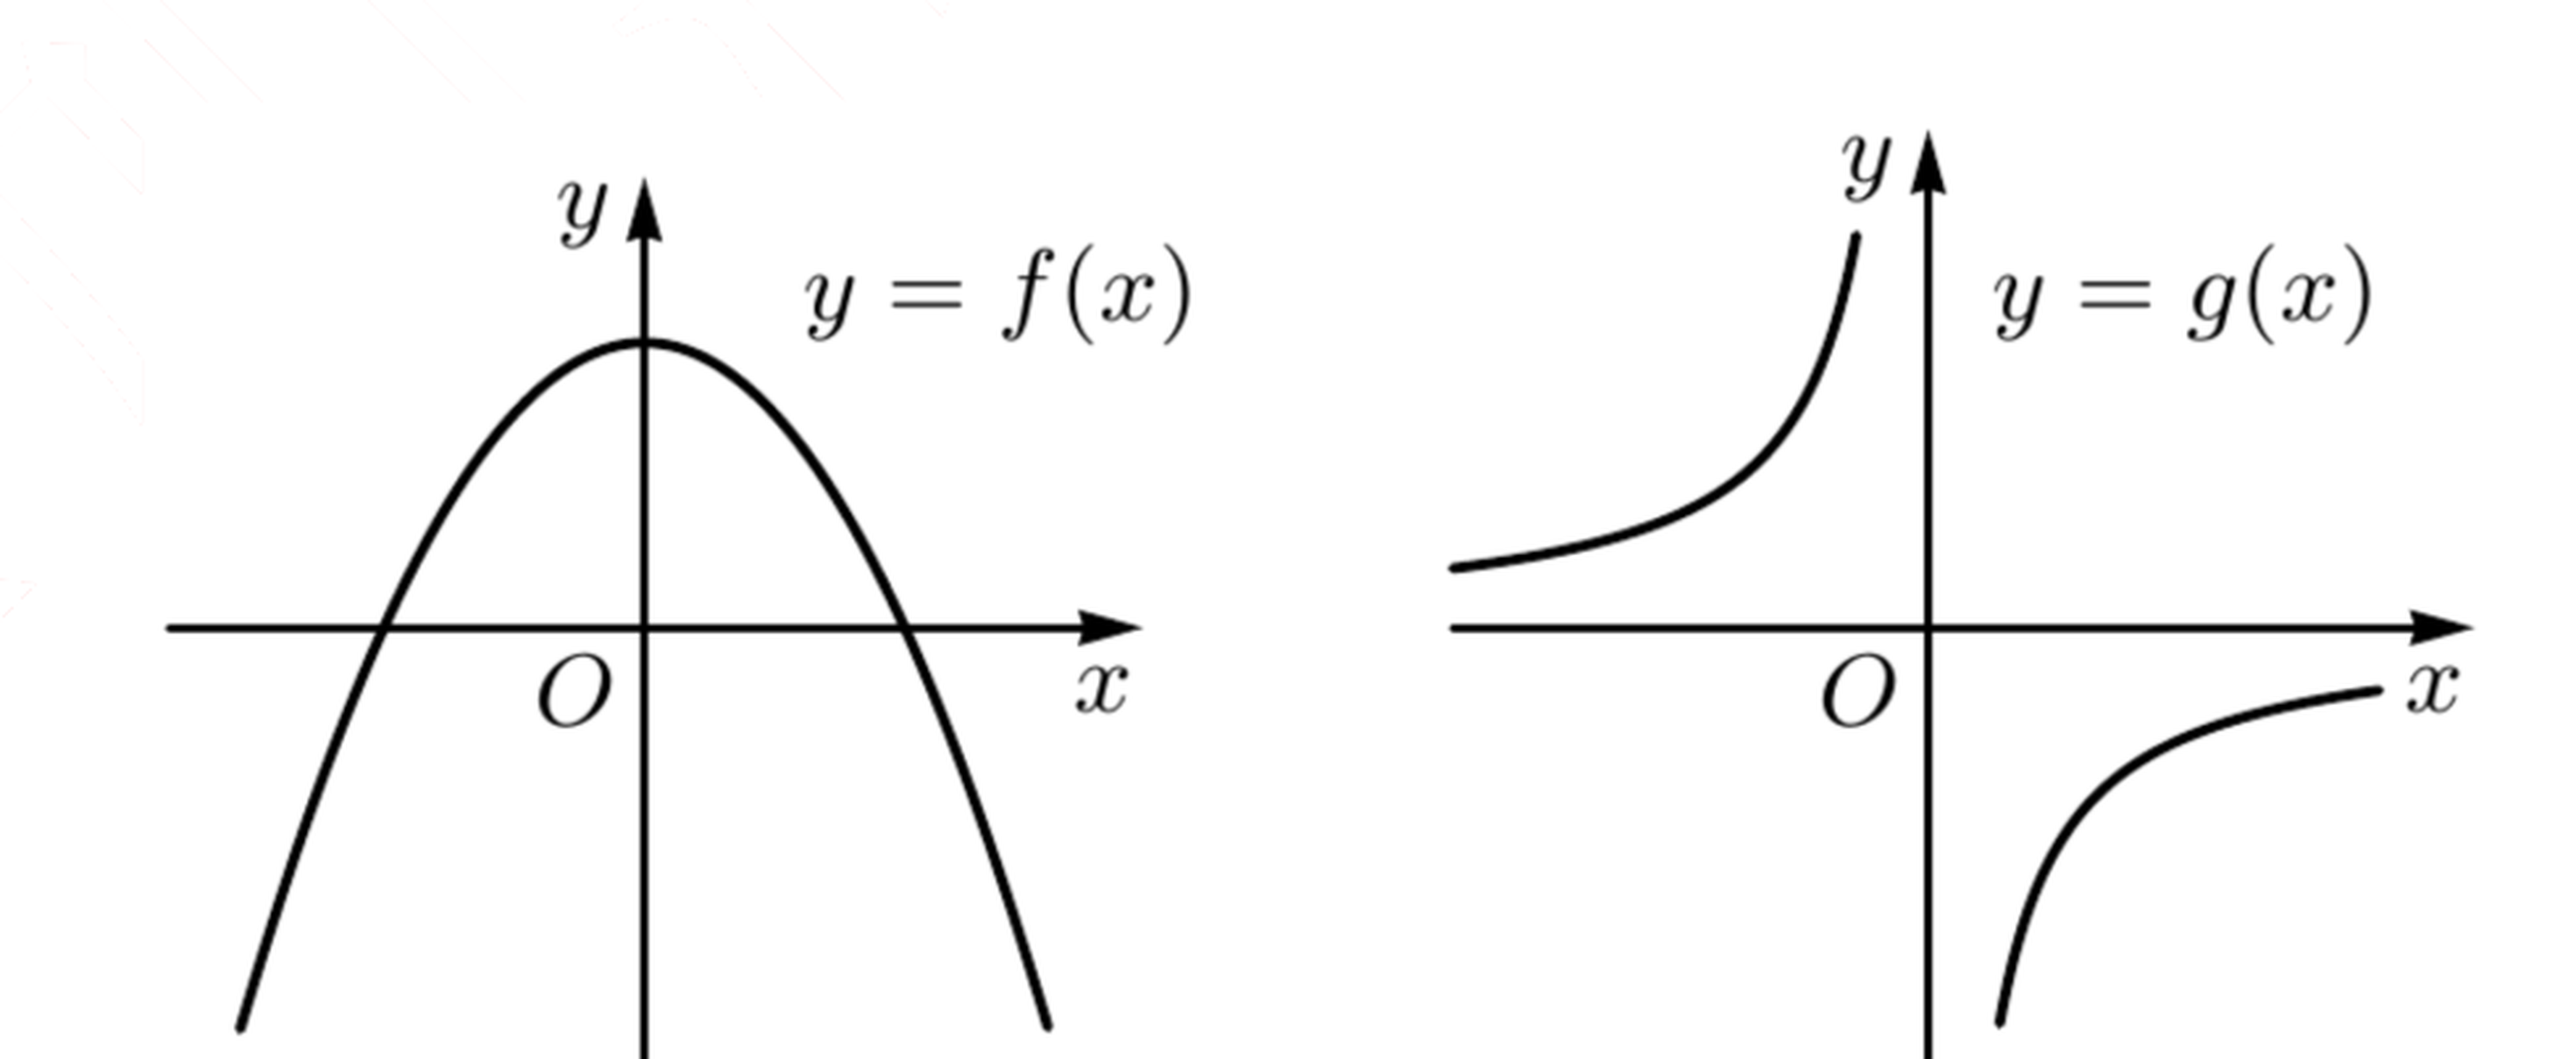
\includegraphics[width=0.72\textwidth]{figures/gao134_q13_graphs.png}\\[0.6em]
% A/B/C/D 四幅函数图象选项取原卷 04 页截图去粉色水印，按原卷一行四幅排布合并为一张
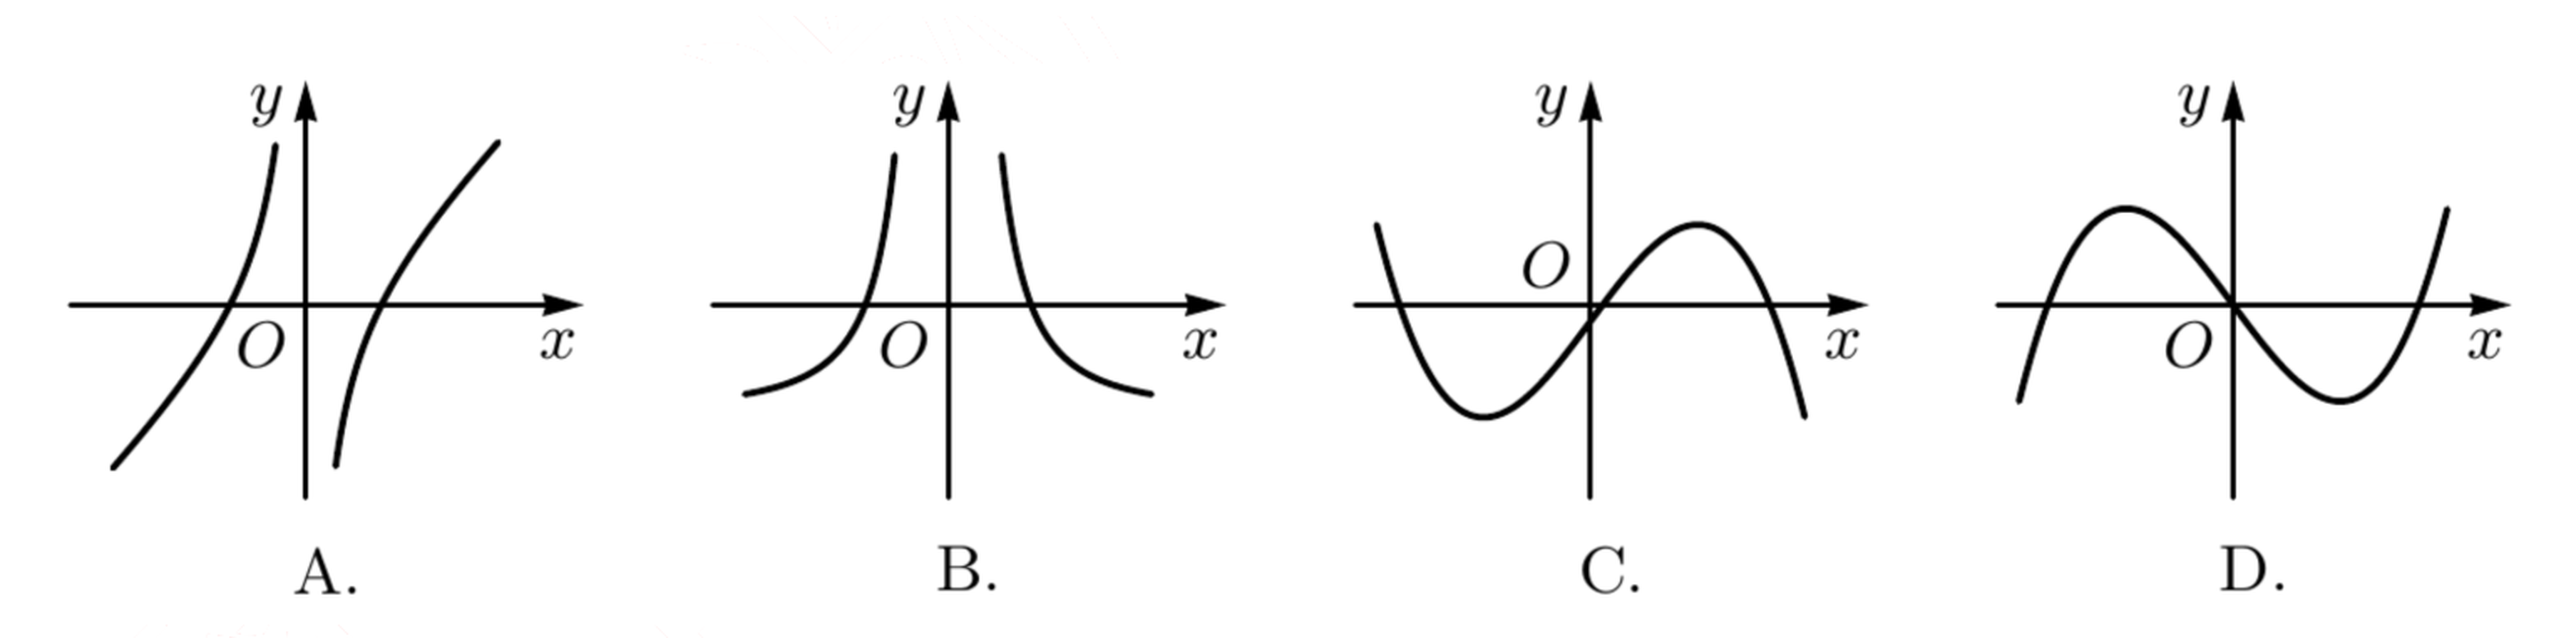
\includegraphics[width=0.90\textwidth]{figures/gao134_q13_options.png}
\end{center}

\ifanswer
\solbegin
\step{$f(x)$ 为偶函数，$g(x)$ 为奇函数，因此 $f(x)g(x)$ 为奇函数，排除 B.}
\step{又 $x=0$ 不在乘积函数的定义域内，其图象在 $y$ 轴上没有点，排除 C、D，}
\step{故选 $A$.}
\solend
\fi

\item 设全集为自然数集 $\N$，$E=\{x\mid x=2n,n\in\N\}$，$F=\{x\mid x=4n,n\in\N\}$，那么集合 $\N$ 可以表示成\mbox{（\quad）}

\keepwithprev
A. $E\cap F$\qquad\qquad B. $\overline{E}\cup F$\qquad\qquad C. $\overline{F}\cup E$\qquad\qquad D. $\overline{E}\cap\overline{F}$

\ifanswer
\solbegin
\step{$F\subseteq E$，所以 $\overline{F}\cup E=\N$，故选 $C$.}
\solend
\fi

\item 已知函数 $y=f(x)$，其中 $f(x)=x^2+bx$，则“$b<0$”是“$f(f(x))$ 的最小值与 $f(x)$ 的最小值相等”的\mbox{（\quad）}

\keepwithprev
A. 充分非必要条件\qquad\qquad B. 必要非充分条件

C. 充分必要条件\qquad\qquad D. 既非充分又非必要条件

\ifanswer
\solbegin
\step{$f(x)=\left(x+\dfrac b2\right)^2-\dfrac{b^2}4$，最小值为 $-\dfrac{b^2}4$，值域为 $\left[-\dfrac{b^2}4,+\infty\right)$.}
\step{当 $b<0$ 时，$-\dfrac b2>0\geqslant-\dfrac{b^2}4$，存在 $x$ 使 $f(x)=-\dfrac b2$，}
\step{从而 $f(f(x))$ 的最小值也为 $-\dfrac{b^2}4$，充分性成立.}
\step{当 $b=0$ 时，$f(x)=x^2$，$f(f(x))=x^4$，两者最小值均为 $0$，必要性不成立.}
\step{故选 $A$.}
\solend
\fi

\item 已知 $a,b,c\in\R$，若存在常数 $M>0$，使得 $a^2+b^2+c^2<M$，则称 $(a,b,c)$ 是有界数组. 对以下两个命题：

①若 $\lvert a^2+b+c\rvert+\lvert a^2+b-c\rvert\leqslant1$，则 $(a,b,c)$ 是有界数组；

②若 $\lvert a^2+b+c\rvert+\lvert a+b^2-c\rvert\leqslant1$，则 $(a,b,c)$ 是有界数组.% ②第二项为 \lvert a+b^2-c\rvert，与①刻意不同，照录

下列判断正确的是\mbox{（\quad）}

\keepwithprev
A. ①和②均为真命题\qquad\qquad B. ①和②均为假命题

C. ①为真命题，②为假命题\qquad D. ①为假命题，②为真命题

\ifanswer
\solbegin
\step{①取 $a=t,b=-t^2,c=0$，条件左端为 $0$，而 $a^2+b^2+c^2=t^2+t^4$ 可任意大，}
\step{故①为假命题.}
\step{②由条件，$a^2+a+b^2+b\leqslant\lvert a^2+b+c\rvert+\lvert a+b^2-c\rvert\leqslant1$.}
\step{由 $(a+1)^2+(b+1)^2\geqslant0$，得 $a^2+b^2\leqslant2(a^2+a+b^2+b)+2\leqslant4$.}
\step{又 $\lvert c\rvert\leqslant\lvert a^2+b+c\rvert+a^2+\lvert b\rvert\leqslant1+4+2=7$，故 $a^2+b^2+c^2\leqslant53<54$，}
\step{可取 $M=54$，故②为真命题.}
\step{故选 $D$.}
\solend
\fi

\end{enumerate}

\bigsec{三、解答题}

\begin{enumerate}
\setcounter{enumi}{16}

\item 已知不等式 $x^2-ax-b<0$ 的解集为 $A$，不等式 $\dfrac{3-2x}{x-1}<0$ 的解集为 $B$.

(1) 若 $a=5$，$b=-6$，求 $A\cap\overline{B}$；

(2) 若 $b=2a^2$，且 $A\cup B=B$，求实数 $a$ 的取值范围.

\ifanswer
\solbegin
\step{(1) 不等式 $\dfrac{3-2x}{x-1}<0$ 等价于 $x<1$ 或 $x>\dfrac32$，}
\step{所以 $B=(-\infty,1)\cup\left(\dfrac32,+\infty\right)$，$\overline{B}=\left[1,\dfrac32\right]$，}
\step{由 $x^2-5x+6=(x-2)(x-3)<0$，得 $A=(2,3)$，因此 $A\cap\overline{B}=\varnothing$.}
\step{(2) $A\cup B=B\Leftrightarrow A\subseteq B$，且 $x^2-ax-2a^2=(x-2a)(x+a)$，}
\step{当 $a=0$ 时，$A=\varnothing$，满足条件.}
\step{当 $a>0$ 时，$A=(-a,2a)$，$-a<0<1$，$A\subseteq B\Leftrightarrow2a\leqslant1$，得 $0<a\leqslant\dfrac12$.}
\step{当 $a<0$ 时，$A=(2a,-a)$，$2a<0<1$，$A\subseteq B\Leftrightarrow-a\leqslant1$，}
\step{得 $-1\leqslant a<0$.}
\step{因此 $a$ 的取值范围为 $\left[-1,\dfrac12\right]$.}
\solend
\fi

\item 为了在夏季降温和冬季供暖时减少能源损耗，房屋的屋顶和外墙需要建造隔热层. 某幢建筑物要建造可使用 $30$ 年的隔热层，每厘米厚的隔热层建造成本为 $9$ 万元. 该建筑物每年的能源消耗费用 $C$（万元）与隔热层厚度 $x$（cm）满足如下关系式：$C=\dfrac{k}{3x+5}$（$0\leqslant x\leqslant10$）. 若不建隔热层，每年能源消耗费用为 $8$ 万元. 设 $y$（万元）为隔热层建造费用与 $30$ 年的能源消耗费用之和.

(1) 求 $k$ 的值及 $y$ 的表达式；

(2) 隔热层修建多厚时，总费用 $y$ 最小？并求最小值.

\ifanswer
\solbegin
\step{(1) 不建隔热层时 $x=0$，$C=8$，所以 $\dfrac k5=8$，得 $k=40$.}
\step{隔热层建造费用为 $9x$ 万元，$30$ 年的能源消耗费用为 $30\times\dfrac{40}{3x+5}$ 万元.}
\step{因此 $y=9x+\dfrac{1200}{3x+5}$，$0\leqslant x\leqslant10$.}
\step{(2) 令 $t=3x+5$，则 $5\leqslant t\leqslant35$，且 $y=3t+\dfrac{1200}{t}-15$，}
\step{因为 $t>0$，由基本不等式得 $y\geqslant2\sqrt{3t\cdot\dfrac{1200}{t}}-15=105$，}
\step{当且仅当 $3t=\dfrac{1200}{t}$，即 $t=20$时取等号，此时 $x=5\in[0,10]$，}% 原卷"20"与"时"之间未留空，照录
\step{所以隔热层厚度为 $5$ cm 时，总费用最小，最小值为 $105$ 万元.}
\solend
\fi

\item 已知 $f(x)=ax^2+\dfrac1x$，其中 $a$ 为常数.

(1) 若 $a\in(1,3)$，判断函数 $y=f(x)$ 在 $[1,2]$ 上的单调性，并用定义证明；

(2) 求函数 $y=f(x)-x-\dfrac1x$ 在 $[1,2]$ 上的最大值 $g(a)$.

\ifanswer
\solbegin
\step{(1) 任取 $x_1,x_2\in[1,2]$，且 $x_1<x_2$，}
\step{则 $f(x_2)-f(x_1)=(x_2-x_1)\left[a(x_1+x_2)-\dfrac1{x_1x_2}\right]$，}
\step{由 $a>1$，$x_1+x_2\geqslant2$，$x_1x_2\geqslant1$，得 $a(x_1+x_2)-\dfrac1{x_1x_2}>2-1>0$，}
\step{因此 $f(x_2)>f(x_1)$，$f(x)$ 在 $[1,2]$ 上为严格增函数.}
\step{(2) 令 $h(x)=f(x)-x-\dfrac1x=ax^2-x$，其中 $x\in[1,2]$.}
\step{若 $a=0$，则 $h(x)=-x$，所以 $h(x)_{max}=h(1)=-1$；}
\step{若 $a<0$，二次函数的图象的对称轴为 $x=\dfrac1{2a}<0$，}
\step{所以 $y=h(x)$ 在 $[1,2]$ 上是严格减函数，所以 $h(x)_{max}=h(1)=a-1$；}
\step{若 $a>0$ 且 $\dfrac1{2a}>\dfrac32$，即 $0<a<\dfrac13$ 时，$h(x)_{max}=h(1)=a-1$.}
\step{若 $a>0$ 且 $\dfrac1{2a}\leqslant\dfrac32$，即 $a\geqslant\dfrac13$ 时，$h(x)_{max}=h(2)=4a-2$.}
\step{综上所述，$g(a)=\begin{cases}a-1,a<\dfrac13\\4a-2,a\geqslant\dfrac13\end{cases}$.}
\solend
\fi

\item 已知 $f(x)=\dfrac{ax^2+1}{bx+c}$（$a,b,c\in\Z$）.

(1) 若函数 $y=f(x)$ 是奇函数，且 $f(1)=2$，$f(2)<3$，求 $a,b,c$ 的值；

(2) 若函数 $y=f(x)$ 是偶函数，且 $ac<0$，$f(2a^2+a+1)<f(-3a^2+2a-1)$，求 $a$ 的值；

(3) 若 $b=a+c^2$，且满足不等式 $\lvert f(x)\rvert\geqslant1$ 的 $x$ 的最大值为 $0$，求 $c$ 的值.

\ifanswer
\solbegin
\step{(1) 由 $f(-x)=-f(x)$，交叉相乘得 $2c(ax^2+1)=0$ 恒成立，}
\step{因此 $c=0$，$b\neq0$.}
\step{由 $f(1)=2$，得 $a+1=2b$，}
\step{于是 $f(2)=\dfrac{4a+1}{2b}=4-\dfrac3{2b}<3\Leftrightarrow0<b<\dfrac32$，}
\step{因为 $b\in\Z$，所以 $b=1$，进而 $a=1$，$c=0$.}
\step{(2) 由 $f(-x)=f(x)$，交叉相乘得 $2bx(ax^2+1)=0$ 恒成立，因此 $b=0$.}
\step{此时 $f(x)=\dfrac ac x^2+\dfrac1c$，且 $\dfrac ac<0$.}
\step{设 $u=2a^2+a+1$，$v=-3a^2+2a-1$.}
\step{方程 $2a^2+a+1=0$ 与 $3a^2-2a+1=0$ 的判别式分别为 $-7$ 与 $-8$，}
\step{都小于 $0$，所以 $u>0$，$v<0$.}
\step{于是 $f(u)<f(v)\Leftrightarrow u^2>v^2\Leftrightarrow u>-v\Leftrightarrow-a^2+3a>0\Leftrightarrow0<a<3$，}
\step{因为 $a\in\Z$，所以 $a=1$ 或 $a=2$.}
\step{(3) 因为解集的最大值为 $0$，所以 $f(0)$ 有定义且 $\lvert f(0)\rvert\geqslant1$，}
\step{即 $c\neq0$，$\left\lvert\dfrac1c\right\rvert\geqslant1$，结合 $c\in\Z$，得 $c=\pm1$，从而 $b=a+1$.}
\step{当 $x=2$ 时，分母 $2a+2+c$ 为奇数，必不为 $0$；}
\step{又因为 $2>0$，必须有 $\lvert f(2)\rvert<1\Leftrightarrow\lvert4a+1\rvert<\lvert2a+2+c\rvert$，}
\step{若 $c=-1$，则 $(4a+1)^2<(2a+1)^2\Leftrightarrow4a(3a+1)<0\Leftrightarrow-\dfrac13<a<0$，}
\step{不存在满足条件的整数 $a$.}
\step{若 $c=1$，则 $(4a+1)^2<(2a+3)^2\Leftrightarrow4(3a+2)(a-1)<0\Leftrightarrow-\dfrac23<a<1$，}
\step{所以 $a=0$，$b=1$，此时 $f(x)=\dfrac1{x+1}$，}
\step{且 $\lvert f(x)\rvert\geqslant1\Leftrightarrow0<\lvert x+1\rvert\leqslant1\Leftrightarrow x\in[-2,-1)\cup(-1,0]$，}
\step{解集的最大值确为 $0$，因此 $c=1$.}
\solend
\fi

\item 已知函数 $y=f(x)$ 的定义域为 $\R$，且当 $x>0$ 时，$f(x)=\dfrac1{x+1}$. 对任意 $x_0\in\R$，定义集合 $D(x_0)=\{d\mid f(x_0+d)>f(x_0)\}$.

(1) 若当 $x\leqslant0$ 时，$f(x)=-2x+1$，求函数 $y=f(x)$ 的值域；

(2) 若 $y=f(x)$ 是偶函数，且 $f(0)=1$，求证：$D(-2)=\{-d\mid d\in D(2)\}$；

(3) 若 $y=f(x)$ 是奇函数，且 $x_1x_2\neq0$，求证：“$f(x_1)\leqslant f(x_2)$”的充要条件是\!\mbox{“$D(x_2)\subseteq D(x_1)$”}.

\ifanswer
\solbegin
\step{(1) 当 $x>0$ 时，$0<f(x)<1$；当 $x\leqslant0$ 时，$f(x)=-2x+1\geqslant1$.}
\step{函数的值域为 $(0,1)\cup[1,+\infty)=(0,+\infty)$.}
\step{(2) 由 $f(x)$ 是偶函数及 $f(0)=1$，得 $f(x)=\dfrac1{1+\lvert x\rvert}$，且 $f(2)=f(-2)=\dfrac13$.}
\stepm{法一：}{$D(2)=\left\{d\mid\dfrac1{1+\lvert2+d\rvert}>\dfrac13\right\}=\{d\mid\lvert2+d\rvert<2\}=(-4,0)$，}
\step{$D(-2)=\left\{d\mid\dfrac1{1+\lvert-2+d\rvert}>\dfrac13\right\}=\{d\mid\lvert-2+d\rvert<2\}=(0,4)$，}
\step{因此 $\{-d\mid d\in D(2)\}=(0,4)=D(-2)$.}
\stepm{法二：}{任取 $d\in D(-2)$，由定义得 $f(-2+d)>f(-2)$.}
\step{因为 $y=f(x)$ 是偶函数，所以对任意的实数 $x$，有 $f(-x)=f(x)$，}
\step{因此 $f(-2+d)=f(-(-2+d))=f(2-d)$，且 $f(-2)=f(2)$.}
\step{所以不等式 $f(-2+d)>f(-2)$ 等价于 $f(2-d)>f(2)$，}
\step{这恰好是 $-d\in D(2)$ 的定义，}
\step{所以 $d\in D(-2)\Leftrightarrow-d\in D(2)$，故 $D(-2)=\{-d\mid d\in D(2)\}$.}
\step{(3) 由 $f(x)$ 是奇函数，得 $f(0)=0$；}
\step{当 $x<0$ 时，$f(x)=-f(-x)=-\dfrac1{1-x}=\dfrac1{x-1}$；}
\step{所以 $f(x)=\begin{cases}\dfrac1{x-1},&x<0\\0,&x=0;\\\dfrac1{x+1},&x>0\end{cases}$}
% 2026-11-15 回原图订正：原卷 11 页此 cases 块末无句点，本稿初转顺手补了西文句点，今删去（Q19 08 页同类块末有句点，照录保留）。
\step{当 $x_0<0$ 时，$D(x_0)=\{d\mid f(x_0+d)>f(x_0)\}=(-\infty,0)\cup[-x_0,+\infty)$，}
\step{当 $x_0=0$ 时，$D(0)=\{d\mid f(0+d)>f(0)\}=(0,+\infty)$，}
\step{当 $x_0>0$ 时，$D(x_0)=\{d\mid f(x_0+d)>f(x_0)\}=(-x_0,0)$.}
\stepm{先证明必要性.}{若 $f(x_1)\leqslant f(x_2)$，仅需讨论三类情形：}
\step{若 $x_2\leqslant x_1<0$，}
\step{则 $D(x_1)=(-\infty,0)\cup[-x_1,+\infty),D(x_2)=(-\infty,0)\cup[-x_2,+\infty)$，}
\step{故 $D(x_2)\subseteq D(x_1)$；}
\step{若 $0<x_2\leqslant x_1$，则 $D(x_1)=(-x_1,0),D(x_2)=(-x_2,0)$，}
\step{故 $D(x_2)\subseteq D(x_1)$；}
\step{若 $x_1<0<x_2$，则 $D(x_1)=(-\infty,0)\cup[-x_1,+\infty),D(x_2)=(-x_2,0)$，}
\step{故 $D(x_2)\subseteq D(x_1)$.}
\stepm{再证明充分性.}{若 $D(x_2)\subseteq D(x_1)$，}
\step{若 $x_1<0,x_2<0$，}
\step{则 $D(x_1)=(-\infty,0)\cup[-x_1,+\infty),D(x_2)=(-\infty,0)\cup[-x_2,+\infty)$，}
\step{由 $D(x_2)\subseteq D(x_1)$ 得 $x_2\leqslant x_1$，}
\step{又 $y=f(x)$ 在 $(-\infty,0)$ 上是严格减函数，所以 $f(x_1)\leqslant f(x_2)$；}
\step{若 $x_1>0,x_2>0$，则 $D(x_1)=(-x_1,0),D(x_2)=(-x_2,0)$，}
\step{由 $D(x_2)\subseteq D(x_1)$ 得 $x_2\leqslant x_1$，}
\step{又 $y=f(x)$ 在 $(0,+\infty)$ 上是严格减函数，所以 $f(x_1)\leqslant f(x_2)$；}
\step{若 $x_1<0,x_2>0$，则 $f(x_1)<0<f(x_2)$，结论成立；}
\step{若 $x_1>0,x_2<0$，此时 $D(x_1)=(-x_1,0)$ 中只有负数，}
\step{而 $D(x_2)=(-\infty,0)\cup[-x_2,+\infty)$ 中有正数，$D(x_2)\subseteq D(x_1)$ 不成立.}
\step{综上，“$f(x_1)\leqslant f(x_2)$”的充要条件是“$D(x_2)\subseteq D(x_1)$”.}
\solend
\fi

\end{enumerate}

\end{document}
